\documentclass[10pt,letterpaper,oneside,professionalfont]{book}
%\usepackage{concrete}

%\usepackage[left=4cm, width=15.50cm, height=23.00cm]{geometry}
\usepackage[width=15.50cm, height=23.00cm]{geometry}
\usepackage[english]{babel}
\usepackage[utf8]{inputenc}
\usepackage[T1]{fontenc}
\usepackage{dsfont}
\usepackage{amsmath}
\usepackage{amsfonts}
\usepackage{amssymb}
\usepackage{graphicx}
\usepackage{paracol}
\usepackage{xparse}
\usepackage{sidecap}
\usepackage[makeroom]{cancel}
\usepackage{capt-of}
\usepackage[margin=1cm]{caption}
\usepackage[dvipsnames]{xcolor}
\usepackage{xpatch}
\usepackage{subcaption}
\usepackage[most]{tcolorbox}
\usepackage{lipsum}
\usepackage{float}
\usepackage{imakeidx}
\usepackage{wrapfig}
\usepackage{marginnote}
\usepackage{ upgreek }
\usepackage{bm}
\usepackage{enumerate}
\usepackage{mathrsfs} 
\usepackage{array}
\usepackage{arydshln}
\usepackage{hyperref}

\graphicspath{{Images/}}


\makeindex[columns=3, title=Indice Analitico, intoc]

\newcolumntype{M}[1]{>{\centering\arraybackslash}m{#1}}
\captionsetup{font = {it, small}, labelfont={color=NavyBlue, bf}}



\newcommand{\F}{\mathscr F}
\newcommand{\four}[1]{\mathscr{F}\left\{ #1 \right\}}
\newcommand{\antifour}[1]{\mathscr{F}^{-1}\left\{ #1 \right\}}
\newcommand{\prob}[1]{\textrm{Pr}\left\{ #1 \right\}}
\newcommand{\intinf}{\int_{-\infty}^\infty}
\newcommand{\infsum}[1]{\sum_{#1=-\infty}^\infty}
\newcommand{\sinc}{\textrm{sinc}}
\newcommand{\rect}{\textrm{rect}}
\renewcommand{\Re}[1]{\textrm{Re}\left\{ #1 \right\}}
\renewcommand{\Im}[1]{\textrm{Im}\left\{ #1 \right\}}
\newcommand{\dft}{discrete Fourier transform }
\newcommand{\fft}{fast Fourier transform }
\newcommand{\circconv}[1]{\underset{\text{\tiny $#1$}} \otimes}
\newcommand{\Z}[1]{\mathcal{Z}\left\{#1\right\}}

\newcommand{\var}[1]{\textrm{Var}\{#1\}}
\newcommand{\dtft}{discrete-time Fourier transform }
\newcommand{\ctft}{continuous-time Fourier transform }

\newcommand{\de}[1]{\textbf{\textcolor{NavyBlue}{#1}}}

\newcommand{\figura}[5]{\begin{SCfigure}[#2][b!h!t!]
		\centering
		\includegraphics[width=#1 cm]{#3}
		\caption{#4} \label{#5}
\end{SCfigure}}





\newcommand{\bfcolor}[1]{\renewcommand*{\textbf}[1]{{\bfseries {\color{#1}##1}}}}
\newcommand{\tabrule}{\rule{\linewidth}{1pt}}

\setcolumnwidth{0.3\textwidth}


\newcounter{domande}
\refstepcounter{domande}
\newcommand{\newquestion}{\vspace{3mm} \noindent \rule{\linewidth}{2pt}\subsection*{Question \thedomande} \refstepcounter{domande}}



\newcounter{concetti}
\newenvironment{concetto}{
	
	\bfcolor{NavyBlue}
	\refstepcounter{concetti}
	{\color{NavyBlue}\textbf{Concetto \theconcetti:}} \quad
}{
}
\numberwithin{concetti}{chapter}
\tcolorboxenvironment{concetto}{
	boxrule=0pt,
	boxsep=0pt,
	colback={White!90!NavyBlue},
	enhanced jigsaw, 
	borderline west={2pt}{0pt}{NavyBlue},
	sharp corners,
	before skip=5pt,
	after skip=10pt,
	breakable,
}

\newcounter{teoremi}
\newenvironment{teorema}[2]{
	\bfcolor{ForestGreen}
	\refstepcounter{teoremi}
	\textbf{Concetto \theteoremi #1} 
	\vspace{3mm} 
	
	\texttt{Ipotesi: } #2
	
	\vspace{3mm} 
	
	\texttt{Enunciato}: 
}{
}
\numberwithin{teoremi}{chapter}
\tcolorboxenvironment{teorema}{
	boxrule=0pt,
	boxsep=0pt,
	colback={White!100!ForestGreen},
	enhanced jigsaw, 
	borderline west={2pt}{0pt}{ForestGreen},
	sharp corners,
	before skip=5pt,
	after skip=10pt,
	breakable,
}


\newenvironment{dimostrazione}{
	\bfcolor{Orchid}
	\textbf{Dimostrazione} \quad
}{ }
\tcolorboxenvironment{dimostrazione}{
	boxrule=0pt,
	boxsep=0pt,
	colback={White!100!NavyBlue},
	enhanced jigsaw, 
	borderline west={2pt}{0pt}{Orchid},
	sharp corners,
	before skip=5pt,
	after skip=10pt,
	breakable,
}

\newenvironment{osservazione}{
	\bfcolor{BurntOrange}
	\textbf{Osservazione: }
}{ }
\tcolorboxenvironment{osservazione}{
	boxrule=0pt,
	boxsep=0pt,
	colback={White!100!BurntOrange},
	enhanced jigsaw, 
	borderline west={2pt}{0pt}{BurntOrange},
	sharp corners,
	before skip=5pt,
	after skip=10pt,
	breakable,
}

\newenvironment{note}{
	\bfcolor{CadetBlue}
	\textbf{Note: }
}{ }
\tcolorboxenvironment{note}{
	boxrule=0pt,
	boxsep=0pt,
	colback={White!100!CadetBlue},
	enhanced jigsaw, 
	borderline west={2pt}{0pt}{CadetBlue},
	sharp corners,
	before skip=5pt,
	after skip=10pt,
	breakable,
}




\newenvironment{proof}{
	\noindent	
%	\renewcommand{\de}[1]{ { \color{ForestGreen} \textbf{#1} } }
	
	{\color{ForestGreen}\textbf{Proof:}}
}{
}
\tcolorboxenvironment{proof}{
	boxrule=0pt,
	boxsep=0pt,
%	colback={White!90!ForestGreen},
	enhanced jigsaw, 
	borderline west={2pt}{0pt}{ForestGreen},
	sharp corners,
	before skip=5pt,
	after skip=5pt,
	breakable,
}


\newcounter{exercises}
\numberwithin{exercises}{chapter}
\newenvironment{exercise}[1]{
	\bfcolor{Periwinkle}
	\noindent
	\refstepcounter{exercises}
	{\color{Periwinkle}\textbf{Exercise \theexercises#1}  } 
	\vspace{3mm}
	
	\noindent
}{
}


\tcolorboxenvironment{exercise}{
	boxrule=0pt,
	boxsep=0pt,
	colback={White!90!Periwinkle},
	enhanced jigsaw, 
	borderline west={2pt}{0pt}{Periwinkle},
	sharp corners,
	before skip=10pt,
	after skip=10pt,
	breakable,
}

\newcounter{examples}
\numberwithin{examples}{chapter}
\newenvironment{example}[1]{
	\bfcolor{Periwinkle}
	\noindent
	\refstepcounter{examples}
	{\color{Periwinkle}\textbf{Example \theexamples#1}  } 
	\vspace{3mm}
	
	\noindent
}{
}


\tcolorboxenvironment{example}{
	boxrule=0pt,
	boxsep=0pt,
	colback={White!90!Periwinkle},
	enhanced jigsaw, 
	borderline west={2pt}{0pt}{Periwinkle},
	sharp corners,
	before skip=10pt,
	after skip=10pt,
	breakable,
}

%\usepackage[defaultfam,light,tabular,lining]{montserrat}
%\renewcommand*\oldstylenums[1]{{\fontfamily{Montserrat-TOsF}\selectfont #1}}

\usepackage[defaultfam,light,tabular,lining]{montserrat}
\renewcommand*\oldstylenums[1]{{\fontfamily{Montserrat-TOsF}\selectfont #1}}
\allowdisplaybreaks

\begin{document}
	
	\frontmatter
	
	\begin{center}
		\vspace{3cm}
		\thispagestyle{empty}
		
\includegraphics[width=5cm]{logouni}
		
		\vspace{1cm}
		\rule{5cm}{0.5pt}
		\vspace{1cm}		
		
		{\Large Università degli Studi di Trento}
		
		\vspace{2cm}
		{\Large Department of Industrial Engineering} \\ \vspace{2mm}
		{\LARGE \textbf{Digital Signal Processing for Mechatronics}} \\ \vspace{2mm}
		{\Large Prof.: Macii David}\\
		
		\vspace{2cm}
		{\LARGE \textbf{Course Notes}}
		
		\vspace{1cm}
		\rule{5cm}{0.5pt}
		\vspace{1cm}	
		
		{\large 
			Matteo Dalle Vedove \\
			\makeatletter
			matteo.dallevedove@studenti.unitn.it
			
			\vspace{2cm}
			Academic Year 2021-2022 \\ \today}
	\end{center}
	
	\tableofcontents
		
	\chapter{Introduction}

	\textbf{06/10/2021}
	
	\paragraph{Energy and power signals} Given a signal $x(t)$ with $t\in [-T/2, T/2]$ or a discrete one $x(n)$ with $n \in [-N/2,N/2]$, we define the \de{energy} $E_T$ and the \de{power} $P_T$ as
	\begin{equation}
	\begin{split}		
		E_T & = \int_{-T/2}^{T/2} |x(t)|^2 \, dt = \sum_{n=-N/2}^{N/2} |x(n)|^2 \\
		P_T & = \frac 1 T\int_{-T/2}^{T/2} |x(t)|^2 \, dt = \frac 1 N \sum_{n=-N/2}^{N/2} |x(n)|^2
	\end{split}
	\end{equation}
	
	This measures are called \textit{energy} and \textit{power} because if we use some physical signals, the evaluation of the integral/sum gives an energy (like for the example the energy/power generated by a voltage source joined by a $1\Omega$ resistor). 
	
	If we push the limit of $T$ we get the \textbf{energy signal} $E = \lim_{T\rightarrow \infty} E_T < \infty$ and the \textbf{power signal} $P = \lim_{T\rightarrow \infty} P_T < \infty$ (note that this 2 values must be limited). This definitions allows us also to define the \de{scalar product between signals}, and in particular for the energy signal it evaluates
	\begin{equation}
		\langle x,y\rangle = \int_{-\infty}^\infty x(t) y^*(t)\, dt
	\end{equation}
	where $y^*$ is the conjugate of the signal $y$. For the power signal instead the definition of the scalar product is described as
	\begin{equation}
		\langle x, y\rangle := \lim_{\Delta t \rightarrow \infty} \frac{1}{\Delta t} \int_{-\Delta t/2}^{\Delta t/2} x(t)y^*(t) \, dt
	\end{equation}
	We can also notice that, for a periodic signal with period $T$ we can consider it's power as $ \frac{1}{T} \int_{-T/2}^{T/2} x(t)y^*(t) \, dt$. And another fact is that the energy of the signal $x(t)$ is defined as $E= \langle x,x \rangle$.
		
	
	\mainmatter
	
	\chapter{Continuous and Discrete-Time Fourier Transform} \label{sec:fourietransforms}
	
	The \de{Fourier transform}, described by the \textit{function} $\F$, is an operator that allows to express a signal $x$ (either continuous depending on the time $t$ or discrete-time depending on the number $n$) in the so called \de{\textit{frequency domain}} ($\Omega$ for continuous-time signals, $\omega$ for discrete-time ones). Such operator can be regarded as the Fourier series, however the difference is that the series operation is performed in the time domain, while the transform operates in the new domain of frequencies.
	
	Given a continuous-time signal $x(t)$ it's \textbf{\ctft} (CTFT) $X(\Omega)$ can be computed as
	\begin{equation} \label{eq:four:ctft}
		X(\Omega) := \int_{-\infty}^{\infty} x(t) e^{-j\Omega t} \, dt \quad \in \mathds C \qquad 
	\end{equation}
	while for discrete-time signals $x(n)$ the definition of the \textbf{\dtft} (DTFT) $X\big(e^{j\omega}\big)$ is
	\begin{equation} \label{eq:four:dtft}
		X\left(e^{j\omega}\right) := \infsum n x(n) e^{-j\omega n} \qquad \in \mathds C
	\end{equation}
	Note that the result of the transform is a complex valued signal, called \de{spectrum}, that can be described by it's \textbf{magnitude} $|X(\Omega)|$ (or $|X(e^{j\omega})|$) and it's \textbf{phase} $\angle X(\Omega)$.
	
	The formal difference between the \textit{continuous frequency} variable $\Omega$ and the \textit{discrete} counterpart $\omega$ lives in their unit of measure: $\Omega$ is in fact expressed as $rad/s$ while $\omega$ is simply expressed as radians. Considering $x(n)$ as a \textit{sampled version} of the signal $x(t)$ with sampling frequency $T_s$, then
	\[ \omega  = \Omega T_s \]
	
	\paragraph{Relationships with other transform} Considering the definition of the Laplace transform
	\[ \mathscr L \big\{ x(t) \} = X(s) := \int_{-\infty}^\infty x(t) e^{-st}\, dt \hspace{2cm} \textrm{with } s = \sigma + j\omega \in \mathds C \]
	that maps a signal into a transfer function in the domain of a complex variable $s$, than it can be observed that the \ctft is the imaginary axis of such plane:
	\[ X(\Omega) = X(s)\Big|_{s=j\Omega} \]
	This means that if a signal has a Laplace transform, then automatically the Fourier one can be determined, while the contrary isn't true  ($x(t)$ can have a Fourier transform but not a Laplace one). Similarly a relation can be seen between the \dtft and the Z transform defined as
	\[ \mathscr Z  \big\{x(n)\big\} = X(z) = \sum_{n=-\infty}^{\infty} x(n) z^{-n}  \hspace{2cm} \textrm{with } z \in \mathds C \]
	In this case the DTFT can be regarded as the evaluation of the Z transform around the unitary circle in the complex plane of the variable $z$:
	\[ X\big(e^{j\omega}\big) = X(z) \Big|_{z=e^{j\omega}}\]
	
	\paragraph{Inverse transform} Every time we have a transform $X$ and important operation that we might want to perform is it's \de{inversion} that allows to reconvert the spectrum into a time-evaluated signal. To perform such operation we can use the formal definition of the \textbf{inverse Fourier transform} that has a slightly difference for continuous and discrete-time original signals:
	\begin{equation} \label{eq:four:inversetransform}
	\begin{aligned}
		x(t) & := \frac 1 {2\pi} \int_{-\infty}^\infty X(\Omega) e^{j\Omega t}\, d\Omega \qquad && \textrm{: continuous-time case} \\
		x(n) & := \frac 1 {2\pi} \int_{-\pi}^\pi X\big(e^{j\omega}\big) e^{j\Omega n}\, d\omega && \textrm{: discrete-time case} 
	\end{aligned}
	\end{equation}
	From this definition is even clearer that, even if $x(n)$ is a discrete-time signal, it's spectrum $X(e^{j\omega})$ is a continuos function; the difference in the inverse Fourier computation between continuous and discrete-time signals is only on the domain on which the integration has to be performed: $[-\infty,\infty]$ in the first case, $[-\pi,\pi]$ in the second.
	
	\paragraph{Existence conditions of the Fourier transform} \label{sec:four:sufficient} In general there's no guarantee that the integral of the Fourier definition converges. No necessary conditions are found in general but we can use a \textbf{sufficient condition} for which {\itshape if a signal $x(t)$ (or $x(n)$) is absolutely summable, then it's transform $X$ exists.} In particular having a absolutely summable signals means that
	\begin{align*}
		& \int_{-\infty}^\infty |x(t)|\, dt < \infty  && \textrm{: continuous-time case} \\
		& \sum_{n=-\infty}^\infty |x(t)|\, dt < \infty \qquad && \textrm{: discrete-time case}
	\end{align*}

	\begin{proof}
		We can use the absolutely summable definition to assert that a spectrum exists considering the following inequalities:
		\[|X(\Omega)| = \left| \int_{-\infty}^\infty x(t) e^{-j\Omega t}\, dt \right| \leq \int_{-\infty}^\infty |x(t)|\, \left|e^{-j\Omega t}\right| \, dt\]
		Having that $|e^{j\Omega t}|$ is always equal to 1, then if the $x$ is infinitely summable than it means that the absolute value of the spectrum must be limited, hence existing.
	\end{proof} \noindent

	While such condition is sufficient to say that a signal surely has a transform, the contrary cannot be said: there are in fact signals that are not absolutely summable but that still presents a Fourier transform.
	
	Considering as example the continuous-time signal $x(t)$ whose spectrum is described by a rectangular distribution $X(\Omega) = \rect_{2\Omega_c} (\Omega)$ (where $\Omega_c = 2\pi f_c$), using the definition of the inverse Fourier transform (equation \ref{eq:four:inversetransform}) we have that
	\begin{equation} \label{eq:four:rectangularinvers}
	\begin{aligned}
		\antifour{X(\Omega)}(t) & = \frac 1 {2\pi} \int_{-\infty}^\infty X(\Omega) e^{j\Omega t}\, d\Omega = \frac 1 {2\pi} \int_{-\Omega_c}^{\Omega_c} e^{j\Omega t}\, d\Omega \\
		& = \frac{e^{j\Omega_c t} - e^{-j\Omega_c t}}{2\pi j t} = \frac{\sin\big(\Omega_c t\big)}{\pi t} \frac{2f_c}{2f_c} = \frac{\sin\big(2\pi f_c t\big)}{2\pi f_c t} 2f_c  \\ 
		& = 2 f_c \sinc\big(\Omega_c t\big)
	\end{aligned}
	\end{equation}
	Determined $\sinc x = \frac{\sin x}{x}$ the \textbf{cardinal sine} function (whose graph is in figure \ref{fig:four:sinc}), it can be shown that such signal is not absolutely summable, however it's transform exists (and is rectangular).
	
	\begin{SCfigure}[2][bt]
		\centering \includegraphics[width=7cm]{sinc}
		\caption{representation of the cardinal sine $sinc(x)$ function.} \label{fig:four:sinc}
	\end{SCfigure}
	
\section{Property of the transform}
	Doing digital signal processing involves a lot of spectral analysis and so it's important to understand the most useful properties related to the transforms and the transforms of common used functions.
	
		In this section (while not otherwise specified) the reported properties are meant to work on both discrete and continuos-time Fourier transform (while still the proof will be presented for only one type of signal).
		
		\paragraph{Linearity} The Fourier transform is a linear operator, meaning that for every signal $x_1(\cdot),x_2(\cdot)$ that has associated transforms $X_1(\cdot),X_2(\cdot)$ and for every constant coefficient $a,b \in \mathds R$, then 
		\begin{equation}
			\four{ax_1(\cdot) + b x_2(\cdot)} = a \four{x_1(\cdot)} + b\four{x_2(\cdot)} = a X_1(\cdot) + bX_2(\cdot)
		\end{equation}
		
		\begin{proof}
			the proof of such properties strictly depends on the linear property of the integrals; expanding the definition of the Fourier transform for continuous-time signals we have
			\[ \int_{-\infty}^\infty \Big(a x_1 (t) + bx_2(t)\Big) e ^{-j\Omega t} \, dt = a \int_{-\infty}^\infty x_1 (t)  e ^{-j\Omega t} \, dt + b \int_{-\infty}^\infty x_2 (t)  e ^{-j\Omega t} \, dt  \]
		\end{proof}
		
		\paragraph{Time shifting} Given a signal $x(t)$ with transform $X(\Omega)$ that's \textit{shifted in time} by a value $t_0$ determining the signal $x(t-t_0)$, then the spectrum of the shifted signal is
		\begin{equation} \label{eq:four:timeshifting}
			\four{x(t-t_0)} = e^{-j\Omega t_0} \four{x(t)} = e^{-j\Omega t_0} X(\Omega)
		\end{equation}
		
		\paragraph{Convolution operator and property} As it will be explained, the behaviour of the output of the system can be regarded as the \textit{convolution} of the input and the impulse response. We so define the \textbf{convolution} operation $x(t)*h(t)$ between the continuous-time signals $x,h$ as 
		\begin{equation}
			y(t) = x(t) * h(t) := \int_{-\infty}^\infty x(\tau) h(t-\tau)\, d\tau
		\end{equation}
		For discrete-time evaluated signals the discrete counterpart of the convolution is defined as
		\begin{equation}
			y(n) = x(n) * h(n) := \sum_{u=-\infty}^\infty x(u) h(t-u)\, du
		\end{equation}
		This operation is commutative, meaning that $x(\cdot)*h(\cdot) = h(\cdot)*x(\cdot)$ and so, while computing the convolution, we can choose the \textit{easier} formulation that simplify the calculations.
	
		With that said the \textbf{convolution property} allows to related the convolution of signals in the time domain as the product of their transforms:
		\begin{equation} \label{eq:four:convolution}
			\four{x(t)*h(t)} = \four{x(t)} \four{h(t)} = X(\Omega) H(\Omega)
		\end{equation}
		
		\begin{proof}
			also in this case the proof can be made by expliciting the definition of the Fourier transform and using properties of the integral calculations:
			\begin{align*}
				\four{x(t) * h(t)} & = \int_{-\infty}^\infty \left( \int_{-\infty}^\infty x(\tau) h(t-\tau)\, d\tau \right) e^{-j\Omega t} \, dt \\
				& =  \int_{-\infty}^\infty x(\tau) e^{-j\Omega \tau} \underbrace{\left( \int_{-\infty}^\infty h(t-\tau) e^{-j\Omega(t-\tau)} \, dt \right)}_{=\four{h(t)}} \, d\tau \\
				& = H(\Omega) \int_{-\infty}^\infty x(\tau) e^{-j\Omega \tau} \, d\tau = X(\Omega) H(\Omega)
			\end{align*}
		\end{proof}
	
		\paragraph{Differentiation in the frequency domain} Another relevant property is related to the differentiation in the frequency domain; given a signal $x(t)$ (but similarly it work for the discrete-time case) with transform $X(\Omega)$ then
		\begin{equation} \label{eq:four:differentiation}
			\four{t\,x(t)} = j \frac{dX(\Omega)}{d\Omega}
		\end{equation}
	
		\begin{proof}
			such property can be proven considering a discrete-time signal $x(n)$; by applying the definition of the \dtft on equation \ref{eq:four:differentiation} we have
			\begin{align*}
				\sum_{n=-\infty}^\infty n x(n) e^{-j\omega n} & = \frac{-j}{-j}\sum_{n=-\infty}^\infty x x(n) e^{-j\omega n}  = j \sum_{n=-\infty}^\infty x(n) \frac{d}{d\omega} \Big(e^{-j\omega n}\Big) \\
				& = j \frac{d}{d\omega}\sum_{n=-\infty}^\infty x(n) e^{-j\omega n} = j \frac{dX(e^{j\omega})}{d\omega}
			\end{align*}
		\end{proof}
		
		\paragraph{Symmetries} Some notable symmetries can be notices while dealing with real evaluated signals $x(\cdot)\in \mathds R$: the transform of such signals are in fact in the form
		\begin{equation}
			X(-\Omega) = X^*(\Omega) \hspace{3cm} X\big(e^{-j\omega}\big) = X^*\big(e^{j\omega}\big)
		\end{equation}
		where $X^*$ is the complex conjugated of $X$.
		\begin{proof} 
			the proof for continuous-time real evaluated signal $x(t)$ can be performed considering the definition
			\begin{align*}
				X(-\Omega) & = \int_{-\infty}^\infty x(t) e^{-j (-\Omega) t} \, dt = \int_{-\infty}^\infty x(t) \left(e^{-j\Omega t}\right)^* \, dt \\ 
				& = \left( \int_{-\infty}^\infty x(t) e^{-j\Omega t} \, dt\right)^* = X^*(t)
			\end{align*}
		\end{proof} \noindent
		
		From this fact we can observe that the \textbf{magnitude spectrum} $|X(\cdot)|$ is always an \textbf{even} function while the \textbf{phase spectrum} $\angle X(\cdot)$ is always \textbf{odd}. From that we can further say:
		\begin{itemize}
			\item if $x(\cdot)$ is real-evaluated and present an event symmetry, then $X(-\Omega) = X(\Omega)$ and the transform is purely real evaluated;
			
			\item if $x(\cdot)$ is real-evaluated and present an odd symmetry, then the complex spectrum $X(\Omega)$ is purely imaginary.
		\end{itemize}
		
		Considering so that every real signal $x(\cdot)$ can be rewritten as the sum $x_e(\cdot) + x_o(\cdot)$ of the following even and odd functions
		\[ x_e(t) = \frac{x(t) + x(-t)}{2} \hspace{3cm} x_o(t) = \frac{x(t) - x(-t)}{2} \]
		then it means that the related spectrum (considering the linearity property) can also be decomposed into a purely real component and an imaginary one:
		\[ X(\Omega) = \int_{-\infty}^\infty x_e(t) \cos(\Omega t) \, dt + j \int_{-\infty}^\infty x_o(t)\, \sin(\Omega t)\, dt = X_e(\Omega) - j X_o(\Omega)\]
		where the results have been obtained using Euler's formula $e^{j\theta} = \cos\theta + j \sin\theta$.
		
		\paragraph{Time reversal} Another property that can be useful is the one that allows to compute the transform of a signal reversed in time; in particular we have that
		\begin{equation}
			\four{x(-t)} = X^*(-\Omega) \hspace{1.5cm} \textrm{and} \hspace{1.5cm} \four{x(-n)} = X^*\big(e^{-j\omega}\big)
		\end{equation}
		
		\begin{note}
			If we also consider that a signal $x(t)$ is real evaluated, using the symmetries relations previously discovered we have that $\four{x(-t)} = X^*(\Omega)$.
		\end{note}
	
	\subsection{Windowing theorem} 
		Assuming to have two signals $x(\cdot),w(\cdot)$  producing the signal $y(t) = x(t) w(t)$, then it's transform can be regarded as the convolution in the frequency domain of the two initial transforms:
		\begin{equation} \label{eq:four:windowing}
			\begin{split}
				\four{x(t)w(t)} & = Y(\Omega) = X(\Omega)*W(\Omega) = \frac 1 {2\pi} \int_{-\infty}^{\infty} X(\Theta) W(\Omega - \Theta)\, d\Theta \\
				\four{x(n)w(n)} & =  Y(e^{j\omega}) = X(e^{j\omega}) * W(e^{j\omega}) = \frac 1 {2\pi} \int_{-\pi}^\pi X(e^{j\theta}) W(e^{j(\omega-\theta)}) \, d\theta
			\end{split}
		\end{equation}
	
		This consideration is important because while dealing with real signals we analyse only one portion (in time) of the signal itself; considering that we can measure a function $x(t)$ in the domain $[0,T]$, then the signal that we have to process is not the complete domain of $x$, but a \textit{truncation} $y(t) = x(t) w(t)$ where $w$ is the so called \textbf{\textit{window}} of the signal that's equal to 1 in the range $[0,T]$ and zero elsewhere. This operation so introduces a distortion in the spectrum of $X$ that depends on the convolution of such transform with the one of the window.
		
		\begin{proof}
			\begin{align*}
				\sum_{n=-\infty}^\infty x(n) w(n) e^{-j\omega n} & = \sum_{n=-\infty}^\infty w(n) \left( \frac 1 {2\pi} \int_{-\pi}^\pi x\big(e^{j\theta}\big) e^{j\theta n} \, d\theta \right) e^{-j\omega n} \\
				& = \frac 1 {2\pi} \int_{-\pi}^\pi \left( X\big(e^{j\theta}\big) e^{j\theta n} \sum_{n=-\infty}^\infty w(n) e^{-j\omega n} \right) \, d\theta \\
				& = \frac 1 {2\pi} \int_{-\pi}^\pi \left( X\big(e^{j\theta}\big)  \sum_{n=-\infty}^\infty w(n) e^{-j(\omega-\theta) n} \right) \, d\theta \\
				& = \frac 1 {2\pi} \int_{-\pi}^\pi X\big(e^{j\theta}\big) W \big(e^{j(\omega - \theta)}\big) \, d\theta
			\end{align*}
		\end{proof}
	
		\paragraph{Parseval's theorem} Corollary to the windowing theorem is the \textbf{Parseval}'s one stating that
		\begin{equation} \label{eq:four:parserval}
			\four{\int_{-\infty}^\infty x(t) y^* (t)\, dt} = \frac 1 {2\pi} \int_{-\infty} ^\infty X(\Omega) Y^*(\Omega)\, d\Omega
		\end{equation}
		Such operation is useful because it allows to calculate in a much easier way the energy $E_x$ of the signal $x(\cdot)$ using the frequency domain:
		\[ E_x = \int_{-\infty}^{\infty} x(t)x(t)\, dt = \frac 1 {2\pi} \int_{-\infty}^\infty X(\Omega) X^*(\Omega) \,d\Omega \]
		
		\paragraph{Correlation} The correlation, described by the operator $\otimes$, is a sort of estimator of the \textit{similarity} (in the time domain) of two signals $x(t),y(t)$ following the equation
		\begin{equation} \label{eq:four:correlation}
			x(t) \otimes y(t) = \intinf x(\tau) y^*(t+\tau)\, d\tau = x(t) * y^*(-t4)
		\end{equation}
		Computing the correlation of the function with itself (so performing $x(\cdot)\otimes x(\cdot)$) gives the \textbf{autocorrelation}. Using Parseval's theorem it can be proven the following relation between correlation and it's transform:
		\begin{equation}
			\four{x(t)\otimes y(t)} = \frac 1{2\pi} \int_{-\infty}^\infty X(\Omega) Y^*(\Omega) e^{j\Omega t} \, d\Omega
		\end{equation}
	
\section{Transforms of standard functions}
	In this section transform of standard function (in both continuous and discrete time domain) are going to be explained.
	
\subsection{Continuous time}
	\paragraph{Dirac pulse} The \textbf{\textit{Dirac's delta}} function $\delta(t)$ is a particular distribution used to model a pulse in the time domain; is characterized by being 0 in all the domain except for $t=0$ that tends to infinity and such that the integral of $\delta(t)$ in all the real axis is unitary. The mathematical definition of such function is
	\begin{equation}
		\delta(t) = \lim_{h\rightarrow 0} \begin{cases}
			\frac 1 h \qquad & 0\leq t \leq h \\
			0 & \textrm{otherwise}
		\end{cases}  \hspace{2cm} \Rightarrow \quad \intinf \delta(t)\, dt = 1
	\end{equation}
	An important property of the Dirac's delta is that the value $g(t_0)$ obtained by the evaluation of the function $g(t)$ at the time $t=t_0$ can be computed 
	\[ g(t_0) = \intinf g(t)\delta(t-t_0) \, dt \]
	
	With such property in mind applying the definition of the \ctft (equation \ref{eq:four:ctft}) of the Dirac pulse can so be regarded as
	\begin{equation} \label{eq:four:impulsetransf}
	\begin{aligned}
		\four{\delta(t)} & = \intinf \delta(t) e^{-j\Omega t}\, dt = e^{-j\Omega 0} \\ & = 1
	\end{aligned}
	\end{equation}
	
	Using also the time shifting property (equation \ref{eq:four:timeshifting}) it's possible to compute the transform of a pulse occurring at any time $t_0$ as $\four{\delta(t-t_0)} = e^{-j\Omega t_0}$; this, from a mathematical point of view, means rotating the complex plane by an angle equal to $\Omega t_0$.
	
	\paragraph{Rectangular and constant signals} Considering a rectangular signal of width $\tau$ centred at the time $t=0$ described by equation
	\[ \rect_\tau(t) = \begin{cases}
		1 \qquad & -\frac \tau 2 \leq t \leq \frac \tau 2 \\ 0 & \textrm{otherwise}
	\end{cases}  \]
	Using this formulation we can compute the transform of the rectangular signal that's
	\begin{equation}
	\begin{aligned}
		\four{A \, \textrm{rect}_\tau(t)}	& =	 A \int_{-\tau/2}^{\tau/2} e ^{-j\Omega t} \, dt = \frac \tau 2 A \frac{e^{-j\Omega \tau/2} - e^{j\Omega \tau/2}}{-j\Omega \frac \tau 2} \\ & = A \tau \sinc (\Omega \tau/2)
	\end{aligned}	
	\end{equation}
	
	A constant signal $x(t) = a$ can be regarded as $\lim_{\tau\rightarrow \infty} a \rect_\tau(t)$ and computing the limits give
	\begin{equation}
	\begin{aligned} \label{eq:four:consttransform}
		\four a & = \lim_{\tau\rightarrow\infty} \four{a \rect_\tau(t)} = \lim_{\tau\rightarrow\infty} a \tau \frac{\sin \left(\frac{\Omega \tau}{2}\right)}{\frac{\Omega \tau}{2}} \\
		& = \delta (\Omega)
	\end{aligned}
	\end{equation}	
	\begin{SCfigure}[2][b]
		\centering 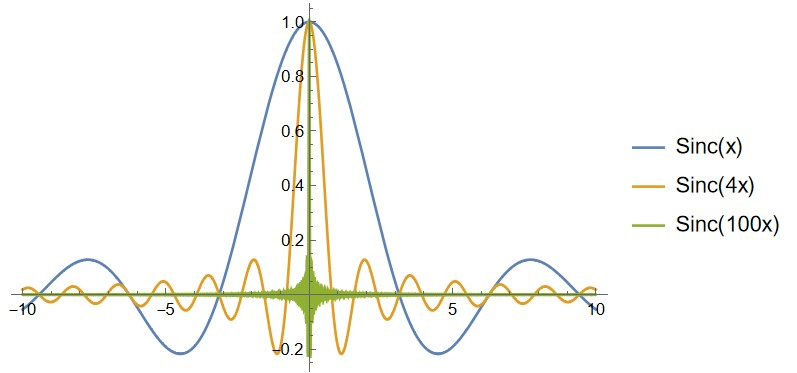
\includegraphics[width=9cm]{sinc-lim}
		\caption{plots of the cardinal sine function $\sinc(n \,t)$ for different values of $n$.} \label{fig:four:sinclim}
	\end{SCfigure}
	As shown in figure \ref{fig:four:sinclim} pushing the limit for the sine function results in a \textit{Dirac's delta distribution-like} function.
	
	\paragraph{Duality principle} Confronting results of equation \ref{eq:four:impulsetransf} and \ref{eq:four:consttransform} we can see that there's a sort of \textit{dual representation}: the transform of a pulse is a unitary signal in the frequency domain while a constant function in the time domain is transformed into a pulse in the frequency domain. This idea is generalized by the \de{duality principle} stating that
	\begin{align*}
		\textrm{if } & X(\Omega) = \four{x(t)} \\
		\textrm{then }& \four{X(t)} = x(-\Omega) \quad \textrm{and} \quad \four{x(\Omega)} = X(-t)
	\end{align*}
	
	\paragraph{Harmonics functions} Considering the case of a generic co-sinusoidal of amplitude $A$, pulsation $\Omega_0$ and initial phase $\phi_0$ determining the signal $x(t) = A \cos(\Omega_0t+\phi_0)$. Applying the definition of the \ctft we determine the spectrum
	\begin{equation}
	\begin{aligned}
		\four{A \cos\big(\Omega_0 t + \phi_0\big)} & = \intinf A  \cos\big(\Omega_0 t + \phi_0\big) e^{-j\Omega t} \, dt \\ 
		& = \intinf A \left( \frac{e^{j(\phi_0 + \Omega_0 t)} + e^{-j(\phi_0 - \Omega_0t)} }{2} \right) e^{-j\Omega t}\, dt \\
		& = \frac A 2 e^{j\phi_0} \lim_{\tau\rightarrow\infty} \int_{-\tau}^\tau e^{j(\Omega_0-\Omega)t}\, dt + \frac A 2 e^{-j\phi_0} \lim_{\tau\rightarrow\infty} \int_{-\tau}^\tau e^{-j(\Omega_0-\Omega)t}\, dt \\
		& = \frac A 2 e^{j\phi_0} \lim_{\tau\rightarrow\infty} 2\tau \sinc\Big(\big(\Omega-\Omega_0\big)t\Big) + \frac A 2 e^{-j\phi_0} \lim_{\tau\rightarrow\infty} 2\tau \sinc\Big(\big(\Omega-\Omega_0\big)t\Big) \\
		& = \frac A 2 e^{j\phi_0} \delta\big(\Omega - \Omega_0\big) + \frac A 2 e^{-j\phi_0} \delta\big(\Omega + \Omega_0\big)
	\end{aligned}
	\end{equation}
	\begin{note}
		to prove such relation the complex notation of the cosine has been used, in fact
		\[ \cos x = \frac{e^{jx} + e^{-jx}}{2} \hspace{3cm} \sin x = \frac{e^{jx} - e^{-jx}}{2} \]
	\end{note} \noindent
	Similarly it can be proven that
	\[ \four{A \sin(\Omega_0 t + \phi_0)} = \frac A {2j} e^{j\phi_0} \delta\big(\Omega - \Omega_0\big) - \frac A {2j} e^{-j\phi_0} \delta\big(\Omega + \Omega_0\big) \]
	
	From this expressions we can see that the transform of sinusoidal functions are described by pulses in the complex frequency domain; in particular the magnitude present Dirac's delta function of amplitude $\frac A 2$ at the frequencies $\pm \Omega_0$ and with a phase depending on $\phi_0$.
	
	\paragraph{Periodic signals} Considering now periodic signals of period $T$, using the Fourier series they can be decomposed into a sum of harmonic signals of the form
	\[ x(t) = \frac{a_0}{2} + \sum_{m=1}^\infty a_m \cos\left( \frac{2\pi m}{T} t \right) + \sum_{m=1}^\infty b_m \sin\left( \frac{2\pi m}{T} t \right) \]
	Applying the yet proven transform of (cos)sinusoidal function then the spectrum of a periodic signal can be regarded as the a sequence of Dirac pulses in the frequency domain in the form:
	\begin{equation}
		X(\Omega) = \frac{a_0}{2} \delta(\Omega) + \sum_{m=1}^{\infty} \frac{a_m - j b_m}{2} \left[ \delta\left( \delta \left( \Omega - \frac{2\pi m}{T}\right) \right) - \delta\left( \Omega + \frac{2\pi m}{T} \right) \right]
	\end{equation}

	\paragraph{Exponential} Let's consider the signal $x(t)$ defined as a exponential only for the positive time range, and so of the form $x(t) = e^{-\alpha t} u(t)$ (where $u(t)$ is the \textit{unit step} that's 1 for $t\geq 0$ and 0 for $t<0$). Considering the sufficient condition described at page \pageref{sec:four:sufficient}, the signal $x(t)$ in order to be transformable needs to have a energy that doesn't diverge: such criteria is matched every time $\alpha >0$. With this assumption the associated transform can be computed as
	\begin{equation}
	\begin{aligned}
		X(\Omega) & = \intinf e^{-\alpha t} u(t) e^{-j\Omega t}\, dt = \int_0 ^\infty e^{-(\alpha + j\Omega) t} \, dt = - \frac{1}{\alpha + j\Omega} e^{-(\alpha + j\Omega) t} \Big|_0^\infty \\
		& = \frac{1}{\alpha + j\Omega}
	\end{aligned}
	\end{equation}
	
	\paragraph{Unit step} Considering the unit step function $u(t)$ defined as
	\begin{equation}
		u(t) = \begin{cases}
			1 \qquad & t\geq0 \\ 0 & t < 0
		\end{cases}
	\end{equation}
	then such function can also be rewritten as the sum of other 2 functions $u_1,u_2$ in the form
	\[ u(t) = u_1(t) + u_2(t) = \frac 1 2 +\frac 1 2 \textrm{sign} (t) \qquad \textrm{where } \textrm{sign(t)} = \lim_{\alpha\rightarrow 0} \begin{cases}
		e^{-\alpha|t|} \qquad &t\geq 0\\
		-e^{-\alpha|t|} \qquad &t< 0\\
	\end{cases} \]
	Using the linear property of the Fourier transform the spectrum $U$ can be regarded as the sum of the spectrum of the constant term $u_1$ (that's $\frac 1 2 \delta(\Omega)$) while the transform of $u_2$ can be regarded as
	\[ U_2(\Omega) = \frac 1 2 \lim_{\alpha\rightarrow0} \left( \frac{1}{a+j\Omega} - \frac{1}{\alpha - j \Omega} \right) = -\frac 1 2 \lim_{\alpha\rightarrow0} \frac{2j\Omega}{\alpha^2+\Omega^2} \]
	Combining the two results we so have that
	\begin{equation}
		U(\Omega) = U_1(\Omega) + U_2(\Omega) = \frac 1 2\delta(\Omega) + \frac{1}{j\Omega}
	\end{equation}
	
	
\subsection{Discrete time}		
	\paragraph{Kronecker pulse} The Kronecker pulse $\delta(n)$ is the discrete-time analogous of the the Dirac's delta distribution and is defined as
	\begin{equation}
		\delta (n) = \begin{cases}
			1 \qquad & n = 0 \\ 0 & n\neq0
		\end{cases}
	\end{equation}
	Similarly to the continuous-time case, it's \dtft it's equal to
	\begin{equation}
	\begin{aligned}
		\four{\delta(n)} & = \infsum n \delta(n) e^{-j\omega n} = e^{-j\omega 0} = 1 \\
		\four{\delta(n-n_0)} & = e^{-j\omega n_0}
	\end{aligned} \hspace{2cm} \forall \omega
	\end{equation}
	where the transform of the shifted pulse is computed considering the related property.
	
	\paragraph{Constant signal} Considering the unitary constant signal $x(n) = 1$ for all $n$ (every constant can be obtained as multiplication of such signal) that can so be described as a \textit{train of Kronecker pulses} in the form
	\[  x(t) = \infsum k \delta(n-k)  \]
	then so it's \dtft can be regarded as
	\begin{equation}
		X\big(e^{j\omega}\big) = 2 \pi \infsum k \delta\big(\omega - 2\pi k)
	\end{equation}
	
	\paragraph{Converging exponential sequence} Considering the case of the exponential sequence $x(n) = a^n u(n)$ only for positive values of $n$, in order to have an absolutely convergent series we must ensure to have $|a|< 1$. With that assumption the \dtft can be computed as
	\[ X\big(e^{j\omega}\big) = \sum_{n=0}^\infty a^n e^{-j\omega n} = \sum_{n=0}^\infty \big(a e^{-j\omega}\big)^n \]
	Considering $a e^{-j\omega} = b$ then this expression can be seen as a convergent geometric series and so
	\begin{equation}
		X\big(e^{j\omega}\big) = \lim_{N\rightarrow \infty} \sum_{n=0}^N b^n = \lim_{N\rightarrow 0} \frac{1-b^{N+1}}{1-b} = \frac 1 {1-b} = \frac{1}{1-ae^{-j\omega}}
	\end{equation}
	\begin{note} \label{sec:four:geometricalprogression}
		Given a geometric series $a_n = q a_{n-1}$ it can be proven that, if $|q| < 1$, the sum of the first $N$ terms is
		\[ \sum_{n=1}^N a_n = \frac{1-q^N}{1-q} \]
	\end{note}
	
	
	
	
	
	
	\chapter{Random Variables and Stochastic Processes}
\section{Probability and random variables}
	Given a \de{random experiment} we define it's \de{sample space} $S$ as the set of all the possible outcomes of such experiment and can be either continuous or discrete; any subset $E\subseteq S$ of the random experiment is called \de{event}.
	
	In order to relate the sample space with the event it's necessary to consider the so called \textit{$\sigma$-algebra} $\mathscr B$ defined on such sample space and that's characterized by the following 3 properties:
	\begin{enumerate}[\itshape i)]
		\item $S \in \mathscr B$, so the sample space is contained in the $\sigma$-algebra domain;
		\item if an event $E \in \mathscr B$, then also it's complement $\overline E = S - E \in \mathscr B$ is contained in the algebraic domain;
		\item for any event $E_i \in \mathscr B$, then the union set $\cup_{i=1}^\infty E_i \in \mathscr B$ lies in the algebraic domain.
	\end{enumerate}

	If all this properties are matched then it's possible to define a \de{probability measure} $P$ in the $\sigma$-algebra with domain $\mathscr B$ that's a function that can be applied to any event $E_i$ (and so $\exists P(E) \forall E \in \mathscr B$) such that
	\begin{enumerate}[\itshape i)]
		\item $0\leq P(E) \leq 1$ 
		\item $P(S) = 1$
	\end{enumerate}
	
	The triplet of the sample space $S$ on which the $\sigma$-algebra $\mathscr B$ is defined as well as the probability measure $P$ is referred as \de{probability space} whose other basic properties are
	\begin{enumerate}[\itshape i)]
		\item $P(\overline E) = 1 - P(E)$;
		\item $P(\emptyset) = 0$ and so $P(S) = 1 - P(\emptyset) = 1$. This means that if $P(E) = 0$ then $E = \emptyset$ and dually if $P(E) = 1$ then $E = S$;
		\item $P(E_1 \cup E_2) = P(E_1) + P(E_2) - P(E_1 \cap E_2)$;
		\item if $E_1 \subseteq E_2$, then $P(E_1) \leq P(E_2)$.
	\end{enumerate}
	
	From page \pageref{sec:probabilityresume} a more detailed description of probability theorems and concepts are described, like the conditional probability and the Bayes theorem.

\section{Random variables}
	A \de{random variable} $X$ can be regarded as a mapping between a sample space $S$ and a \textbf{real} or \textbf{discrete} axis
	\begin{align*}
		X&: S \in \mathscr B \rightarrow \mathds R  && \text{continuous random variable} \\
		X&: S \in \mathscr B \rightarrow \mathds Z  && \text{discrete random variable} 
	\end{align*}
	Associated at the concept of random variable $X$ is the \de{cumulative distribution function}  CDF $F_X(x), f_{cd,X}(x)$ that measures the probability of having random values $X$ less then a certain threshold $x$:
	\[ F_X(x) = f_{cd,X}(x) := P \big\{ X \leq x \big\} \]
	By a mathematical point of view such value is computed differently for continuous of discrete random variables and in particular
	\begin{equation} \label{eq:prob:cdf}
	\begin{aligned}
		f_{cd,X}(x)& := \int_{-\infty}^x f_{pd,X}(\xi)\, d\xi   \qquad && \text{continuous random variable} \\
		f_{cd,X}(x)& := \sum_i^{n_x} p_i && \text{discrete random variable} 
	\end{aligned}
	\end{equation}
	where $f_{pd,X}(x)=f_X(x)$ is the \de{probability density function} PDF that's used to known the \textbf{\textit{distribution}} of a continuous random variable; for a discrete random variables it's instead used the \de{probability mass function} $p_i$ that states the probability of having an event equal to the $i$-th discrete value of the sample space.	
	
	\paragraph{Median} We define the \de{median} $\textrm{med}$ of a random variable the value whose probability of occurring is $50\%$ and so 
	\begin{equation}
		P\big\{ x \leq \textrm{med} \big\} = \frac 12
	\end{equation}
	
	\subsection{Statistical moment of random variable}	
		Given a random variable $X$ it's possible to compute it's $r$-th \de{raw statistical moment} using the \textbf{expectation} operator $E\{X^r\}$ defined as:
		\begin{equation}
		\begin{aligned}
			E\{X^r\}& := \intinf x^r f_{pd,X}(x)\, dx   \qquad && \text{continuous random variable} \\
			E\{X^r\}& := \sum_i x_i^r p_X(x_i) && \text{discrete random variable} 
		\end{aligned}
		\end{equation}
		
		Directly descenting from this concept is the \de{central statistical moment} (of order $r$) defined as the raw statical moment of the same order but evaluated respect on the \de{mean value} $\mu$ of the distribution:
		\begin{equation}
			\text{$r$-th central statistical moment:} \qquad E\left\{ (X-\mu)^r \right\}
		\end{equation}
		In particular the mean value can be computed as the 1$^{st}$ raw statistical moment of the random variable $E\{X\} = \mu$ and represent the \textit{centrality of a process}, the centroid of the probability density function.
		
		The raw statistical moment of order 2 $E\{X^2\}$ or a random variable evaluates as it's \textbf{power} and is useful in particular physical application; the third order moment $E\{X^3\}$ computes instead the so called \textbf{\textit{skewness}}, a parameter representing the \textit{symmetry} in the distribution. \vspace{3mm}
		
		Considering instead the central statistical moment, if evaluated at the first order the result is always zero (it's proven that the expectation operator is linear and so $E\{X-\mu\} = E\{X\} - \mu = \mu - \mu =0$), while the second order one allows to compute the \de{variance} $\sigma^2$ of the distribution so defined as
		\begin{equation}
		\begin{aligned}
			\sigma^2 & = E\big\{ (X-\mu)^2 \big\} = E\{X^2\} - E\{2\mu X\} + E\{\mu^2\} \\
			& = \textrm{power} - 2 \mu E\{X\} + \mu ^2 \\ & = \textrm{power} - \mu^2
		\end{aligned}
		\end{equation}
		This coefficient measures the \textit{dispersion} of the probability distribution respect to the mean value od the distribution itself.
	
	\subsection{Characteristic function}
		An useful operator used in the analysis of a random variable $X$ is the so called \de{characteristic function} $\Gamma_X(\Omega)$ defined as
		\begin{equation}
			\Gamma_X(\Omega) := \intinf f_{pd,X}(x) e^{j\Omega x}\, dx \qquad \in \mathds C
		\end{equation}
		We can observe that such definition is similar to the one of the \ctft (equation \ref{eq:four:ctft}, page \pageref{eq:four:ctft}) with the different that the signal $x$ is not time dependent but can be a generic function. This characteristic function can be used to compute every raw statistical moment using the expression
		\begin{equation}
			E\big\{ X^r \big\} = \frac{1}{j^3}  \left. \frac{d^r}{d\Omega^r} \Gamma_X \right|_{\Omega= 0}
		\end{equation}
		
		\paragraph{Example} Considering as example a gaussian distribution with mean $\mu$ and variance $\sigma^2$, the associated characteristic function is
		\[ \Gamma_X(\Omega) = e^{j\Omega \mu - \frac{\Omega^2\sigma^2}{2}} \]
	
	\subsection{Multiple random variables}
		Let's now consider the case of two random variables $X$ and $Y$ defined in the same sample space $S$: the analogous of the CDF defined in equation \ref{eq:prob:cdf} (page \pageref{eq:prob:cdf}) is the \textbf{joint cumulative density function} $F_{XY}$ that takes into account the interactions that might occur between the two variables:
		\begin{equation}
			F_{XY} (x,y) = f_{cd,XY} (x,y) = P\big\{ X\leq x \textrm{ and } Y \leq y \big\} := \int_{-\infty}^x \int_{-\infty}^y f_{pd,XY}(u,v)\, du\, dv
		\end{equation}
		The associated \textbf{joint probability density function} of the two random variables is so
		\begin{equation}
			f_{pd,XY} := \frac{\partial^2}{\partial x\, \partial y} f_{cd,XY}
		\end{equation}
		Properties of such distributions are:
		\begin{enumerate}[\itshape i)]
			\item $f_{cd,XY} (x,\infty) = f_{cd,X}(x)$ and $f_{cd,XY} (\infty,y) = f_{cd,Y}(y)$ and this expressions represent the \textit{marginal cumulative density functions};
			\item $f_{pd,X}(x) = \intinf f_{pd,XY}(x,y)\, dy$ and $f_{pd,Y}(y) = \intinf f_{pd,XY}(x,y)\, dx$ and this expressions represent the \textit{marginal probability distribution function};
			\item it has $\intinf \intinf f_{pd,XY}(x,y)\,dx\,dy = 1$.			
		\end{enumerate}
	
		The concept of \textbf{conditional probability} can be extended for multiple random variables as
		\begin{equation}
			f_{X|Y}(y|x) = \begin{cases}
				\frac{f_{pd,XY}(x,y)}{f_{pd,X}(x)} \qquad & f_{pd,X}(x) \neq 0 \\
				0 & \textrm{otherwise}
			\end{cases}
		\end{equation}
		As shown in the probability section, if the conditional probability $f_{Y|X} (x,y)$ is equal to  $f_{pd,Y}(y)$, then the two random variables $X$ and $Y$ are statistically independents and
		\[ f_{pd,XY}(x,y) = f_{pd,X}(x) f_{pd,Y}(y) \]
		 Also the statistical moments of $r$-th order can be described for multiple random variable for both the raw and central estimators using the operators
		 \begin{equation}
		 \begin{aligned}
		 	\text{raw statistical moment:} \qquad & E\big\{ X^rY^r \big\} = \intinf \intinf x^r y^r f_{pd,XY}(x,y)\, dx \,dy \\
		 	\text{central statistical moment:} \qquad & E\big\{ (X-\mu_X)^r(Y-\mu_Y)^r \big\} 
		 \end{aligned}
		 \end{equation}
		
		\paragraph{Correlation and covariance}	With the definition of the raw statistical moment we can define the \de{correlation} $\phi = E\{XY\}$ of the two random variable, a parameters that measures the \textit{correlation} between the two random variables; in the extreme case when $\phi = E\{X\} E\{Y\}$ then the random variables are not correlated.
		\begin{note}
			In general having two statistically independent random variable results in zero correlation, however the contrary isn't true: it might happen that $\phi = 0$ but $X,Y$ are statistically dependent!
		\end{note}
		The 1$^{st}$ order central statistical moment is instead used to compute the \de{covariance} $C = E\{ (X-\mu_Y)(Y-\mu_Y) \}$ of those variables; note that if $\mu_X= \mu_Y = 0$, then the covariance $C=\phi$ is equal to the correlation; if it happens that $X,Y$ are also uncorrelated, then the covariance $C$ is zero.
		
		To check the \textit{independence} (uncorrelation) between the two variable \textbf{scatter diagrams} can be used; such diagram relates an outcome of $X$ with respective outcome on $Y$ and:
		\begin{itemize}
			\item if the diagrams shows a \textit{circular cloud} of points, then the two variables are uncorrelated;
			\item if the points in the scatter plot can be interpolated by a function (such a linear equation $y = ax +b$), then the two variables are perfectly correlated.
		\end{itemize}
		To better evaluate the \textit{relationship} between the variables it can be used the \textbf{correlation coefficient} $\rho$ defined as
		\begin{equation}
			\rho = \frac{C(X,Y)}{\sigma_X \sigma_Y}
		\end{equation}
		When $\rho = 0$ then the variables are uncorrelated while in the other extreme when $\rho = \pm 1$ the random variables are perfectly correlated.
		
		\vspace{3mm}
		
		\textbf{MANCHEREBBE DEFINIZIONE E PROPERIETA VARIANZA, JOINTLY GAUSSIAN RANDOM VARIABLES}
	
\section{Stochastic processes}
	A \de{random} (stochastic) \de{process} can be regarded as
	\begin{itemize}
		\item a collection of continuous/discrete time functions that are related to the outcomes of a given sample space $S$ with a certain statistical distribution; each function is called \de{realization} of the random process;		
		\item a collection of random variables that changes with time.
	\end{itemize}
	
	\begin{SCfigure}[2][bt]
		\centering 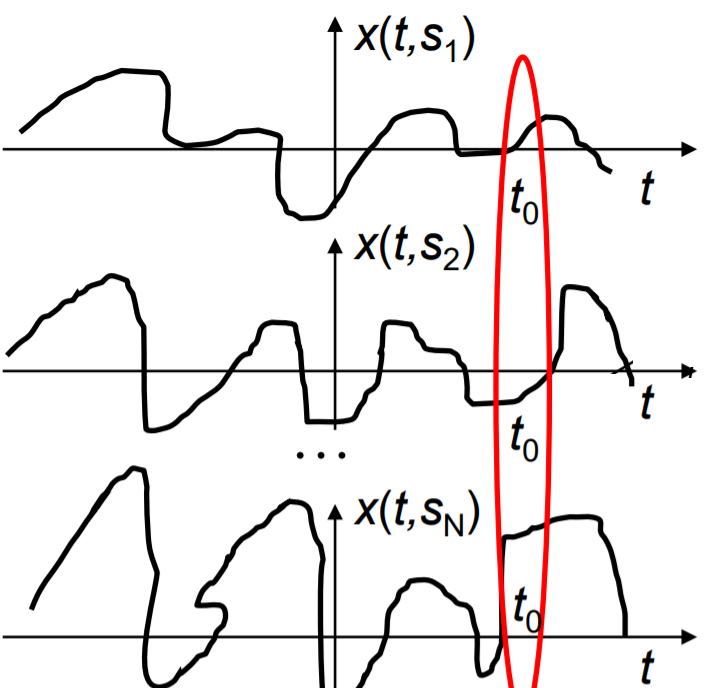
\includegraphics[width=5.5cm]{randomprocesses}
		\caption{scheme to refer while dealing with random processes.} \label{fig:prob:randomprocesses}
	\end{SCfigure} \noindent

	Considering the example in figure \ref{fig:prob:randomprocesses}, every function $x(t,s_i)$ is a realization of the stochastic process while instead the set of all the values read at a certain time (red circle) $x(t_0,s_1)$, $\dots$, $ x(t_0,s_N)$ can be regarded as a random variable $X(t_0)$ extracted from the random process.

	With a description of the stochastic process considering the outcomes $X(t)$ of the random variable changing in time, the relationship between 2 or more random variables $X(t_n)$, $\dots$,  $X(t_s)$ is described by the \textbf{joint probability density function} $f_{pd,X_n\dots X_s}$ for continuous RV or using the joint probability mass function in the discrete-time case.
	
	A complete statistical description of a stochastic process requires to know the joint PDF/PMF of $X(t_n),\dots X(t_s)$ for any tuple of timestamps $(t_n,\dots, t_s)$ and this relations are in general very difficult to be determined.\\
	A weaker condition that allows to describe a random process is instead by knowing the $M^{th}$ order statistic of the joint PDF/PMF of any tuple of random variables $X(t_n),\dots, X(t_s)$ with size $n \leq M$; also those computation can quickly escalates, but in practise with $M=2$ the associated description of the random phenomenon is quite good. The joint CDF for the case $M=2$ is so
	\begin{equation}
		\begin{aligned}
		f_{cd,X_nX_m} (x_n,x_m) & =  \left\{ \begin{aligned}
			& \int_{-\infty}^x \int_{-\infty}^y f_{pd, X_nX_m} (x_n,x_m)\, dx_n\, dx_m && \text{continuous r.v.}\\
			& \sum_j^y \sum_i^x p_{X_{n_i}X_{m_j}} && \text{discrete r.v.}
		\end{aligned} \right. \\
		P\big\{ X(t_n) \leq x, X(t_m) \leq y \big\} & =
		\end{aligned}
	\end{equation}
	If the random variables extracted by the stochastic process are statistically independents then the marginal distribution of each random variable doesn't effect the PDF of the other and in particular we have that
	\begin{equation}
		f_{pd,X_n\dots X_s} (x_n\dots, x_s) = f_{X_n}(x_n) \dots f_{X_s}(x_s) 
	\end{equation}
	
	\paragraph{Example of stochastic process} Let's consider now the random process defined by the random variable
	\[ X(t) = A \cos(\Omega_0 t + \Theta) \]
	where $\Omega_0 \in \mathds R$ is a constant parameter while instead $\Theta$ is another random variable uniformly distributed in the range $[0,2\pi]$ having so the following probability density function:
	\[ f_{pd,\Theta}(\theta) = \begin{cases}
		\frac 1 {2\pi} \qquad & \theta\in[0,2\pi] \\ 0 & \textrm{otherwise}
	\end{cases} \]
	In this case $X(t)$ is a random process: it has a analytical description defined by the cosine function $g(t,\Theta) = \cos(\Omega_0t + \Theta)$ but also has a stochastic contribution depending on the random value of the phase $\Theta$. 
	
	Considering this problem, the goal is to define the probability density function $f_{pd,X}(x(t))$ of the stochastic process, the mean value $\mu(t)$ and the autocorrelation $\phi(t_1,t_2)$ of the function at two different times:
	\begin{enumerate}[a)]
		\item to determine the PDF of the stochastic process we can consider that the argument $\Omega_0 t + \Theta$ of the cosine can be regarded as a unique random variable $\Psi$ uniformly distributed in the range $[0,2\pi]$ for a specific timestamp $t$:
		\[ f_{pd,\Psi}(\psi) = \begin{cases}
			\frac 1 {2\pi} \qquad & \psi\in[0,2\pi] \\ 0 & \textrm{otherwise}
		\end{cases} \]
		Rewriting the random process as $x(t) = A \cos\Psi$, by inverting this equation we can determine the value of the variable $\psi$ as function of the output $x$ as
		\[ \psi= \arccos \left(\frac x A\right) \]
		For every value $x/A$ in the domain $[-1,1]$ such relation gives two solutions in the form $\psi_2 = 2\pi - \psi_1$; knowing so the deterministic function that determines $X$ from the random variable $\Psi$, then the probability density function can be determined using equation \textbf{AGGIUNGERE EQUAZIONE E RIFERIMENTO IN PRECEDENZA} as
		\begin{align*}
			f_{pd,X}(x) & = \sum_{i=1}^2  \frac{f_{pd,\Psi}(\psi_i)}{|g'(\psi_i)|} = \frac 1 {2\pi} \frac{1}{A \sin \psi_1} + \frac 1 {2\pi} \frac{1}{A \sin \psi_2} \\
			& = \frac{1}{2\pi A \sin\left(\arccos \frac x a\right)} + \frac{1}{2\pi A \sin\left(2 -\arccos \frac x a\right)} 
			= \frac1{2\pi A} \left( \frac 1 {\sqrt{1- \left( \frac x A \right)^2 }} + \frac 1 {\sqrt{1- \left( \frac x A \right)^2 }} \right) \\ & = \frac 1 {\pi A\sqrt{1- \left( \frac x A \right)^2 }}
		\end{align*}
		where $g(\psi) = A  \cos(\psi)$ and the property $\sin(\arccos x) = \sqrt{1-x^2}$ has been considered. We can now see that the probability density function can be computed  only when $|x|\leq A$ and in particular
		\[ f_{pd,X}(x) = \begin{cases}
			\frac 1 {\pi \sqrt{A^2-x^2}} \qquad & |x| \leq A \\
			0 & |x|>A
		\end{cases} \]
		Observing that $\Psi$ doesn't depend on time, the PDF of the random variable $X$ isn't either.
		
		\item The mean value of the random process can be trivially calculated by using the first raw statistical moment on the yet found probability density function:
		\[ \mu(t) = \mu = \intinf x f_{pd,X}(x)\, dx = 0 \]
		due to the symmetry of the PDF. The same result could have been obtained considering the deterministic function that related the dependent random variable $X$ with the independent one $\Psi$ using equation \textbf{AGGIUNGERE EQUAZIONE E RIFERIMENTO}:
		\[ \mu = \intinf g(\psi) f_{pd,\Psi}(\psi) \, d\psi = \int_0^{2\pi} A \cos\psi \frac{2 }{2\pi} \, d\psi = \frac A {2\pi} \sin \psi \Big|_{0}^{2\pi} = 0 \]
		
		\item The autocorrelation $\phi(t_1,t_2)$ can be instead calculated using the first order raw statistical moment on two random variables $X(t_1),X(t_2)$ extracted at two different times:
		\begin{align*}
			\phi_X(t_1,t_2) & = E\big\{ A \cos \big(\Omega_0 t_1 + \theta \big) A \cos \big(\Omega_0 t_2 + \theta \big) \big\}
		\end{align*}
		using the linearity property of the expectation operator $E\{\cdot\}$ and using the trigonometric expansion $\cos \alpha \cos \beta = \frac 1 2 \cos(\alpha + \beta) + \frac 1 2 \cos(\alpha - \beta)$ we have		
		\begin{align*}
			\phi_X(t_1,t_2) & = A^2 \, E\left\{ \frac 1 2 \cos \Big( \Omega_0(t_1-t_2) \Big) + \frac 1 2 \cos \Big( \Omega_0 (t_1+t_2) + 2\theta \Big) \right\} \\
			& = \frac {A^2}2 \cos\Big(\Omega_0 (t_1-t_2)\Big) + \frac {A^2}2 \cancelto{0}{E \left\{\cos \Big( \Omega_0 (t_1+t_2) + 2\theta \Big) \right\} }
		\end{align*}
	\end{enumerate}
	
	\subsection{Classification of stochastic processes: stationary cases}
		\paragraph{Strict-sense stationary} As previously seen, a stochastic process can be regarded as a collection of random variables that might change over time; every time a random process has all joints PDF/PMF that are time invariant, then it's defined as \de{strict-sense stationary} and it has that
		\[ f_{pd, X_n} (x_n) = f_{pd,X_{n+k}} (x_{n+k}) \quad \textrm{and} \quad f_{pd, X_n X_m} (x_n, x_m) = f_{pd,X_{n+k}X_{m+k}} (x_{n+k}, x_{m+k}) \qquad \forall k \]
		Having that the probability density function (or the PMF in the discrete case) is always constant over time it descent that also all the properties of the distribution (such mean $\mu$ and variance $\sigma^2$) are constant. Having strict-sense stationary processes is usually impossible in real life and happens only upon strong theoretical hypothesis; for engineering applications most processes are however approximated as strict-sense stationary.
		
		\paragraph{Wide-sense stationary} A process is instead defined as \de{wide-sense stationary} if just the mean of any random variable extracted from the process itself is independent from the time and the correlation depends just on the  time difference between the pair of random variables, so:
		\begin{align*}
			& \mu_n = E\{ X(t_n) \} = \mu = \textrm{constant} \\
			& \phi_X (t_n,t_m) = E\{ X(t_n) X(t_m) \} = \phi_X \big(t_n-t_m\big) \qquad \forall t_n,t_m
		\end{align*}
		
		From this definition we can see that a strict-sense stationary process it's also wide-sense stationary, while the contrary isn't true in general. \\
		We define as \textbf{autocorrelation} $\phi_X$ the correlation between random variables extracted from the same stochastic process, while if they came from different random processes the correlation is called \textbf{cross-correlation}. For wide-sense stationary processes we have the following properties for the autocorrelation:
		\begin{align*}
			i) \qquad & \phi_X (t_m) = \phi_X (-t_m) && \forall t_m \\
			ii) \qquad & \phi_X(0) = E\{ X^2(t_m)\} && \forall t_m \\
			iii) \qquad & |\phi_X(t_m)| \leq \phi_X(0)
		\end{align*}
		Property $ii)$ describes that for any wide-sense stationary process the \textbf{expected} (average) \textbf{power} $E\{X^2(t_m)\}$ of the stochastic process $X$ at any time $t_m$ can be regarded as the autocorrelation $\phi_X(0)$ of the signal for $\tau = 0$ and this value is strictly positive; property $iii)$ express that the autocorrelation for $\tau = 0$ is the upper bound of the autocorrelation function $\phi_X(\tau)$.
		
		
		\begin{example}{: wide-sense stationary process}
			Considering the random process $X(t)$ defined as
			\[ X(t) = \cos(t + U) \hspace{2cm} U \backsim \mathcal U(0,2\pi) \]
			where so $U$ is a random variable uniformly distributed in the range $[0,2\pi]$, in order to prove it's wide-sense stationarity we firstly need to check that its mean is time invariant by so computing the first order raw statistical moment:
			\[ \mu_X(t) = E\{X(t)\} = E\{ \cos(t + U) \} = \int_0^{2\pi} \cos(t+u) \frac 1 {2\pi}\, du = 0 \quad \forall t\in \mathds R \]
			
			Verified this condition we now have to check the autocorrelation of the signal by computing the joint raw statistical moment of the random variable at different times:
			\[\phi_X(t_1,t_2) = E\{ X(t_1) X(t_2) \} = E\{ \cos(t_1 + U) \cos(t_2 + U) \} \]
			Using trigonometric rules we obtain that
			\begin{align*}
				\phi_X(t_1,t_2) & = E\left\{ \frac 1 2 \cos(t_1+t_2+2U) + \frac 1 2 \cos(t_1-t_2) \right\} \\
				& = \cancelto{0}{\int_0^{2\pi} \frac 1 2 \cos(t_1 + t_2 + 2u)\frac 1{2\pi}\, du} + \frac 1 2 \cos(t_1-t_2)
			\end{align*}
			We can so observe that the autocorrelation function only depends on the time difference $\tau = t_1-t_2$ between the evaluation of the signal and can so be regarded as
			\[ \phi_X(t_1,t_2) = \phi_X(\tau) = \frac 1 2 \cos \tau \]
			With this condition satisfied we verified that $X(t)$ is a wide-sense stationary process.			
		\end{example}
		
		\paragraph{Cyclo-stationarity} A stochastic process is defined as \de{cyclo-stationary} (with period $T_0$) iw both mean $\mu$ and autocorrelation $\phi$ are periodic with period $T_0$, so
		\begin{align*}
			i) \qquad & \mu(t+ kT_0) = \mu(t) && \forall k\in\mathds Z \\
			ii) \qquad & \phi_X(t+\tau+kT_0, t+kT_0) = \phi_X(t+\tau,t) && \forall \tau \in \mathds R , \ \forall k\in \mathds Z
		\end{align*}
		Example of cyclo-stationary random process is $Y(t) = X(t) \cos(\Omega_0 t)$ where $X(t)$ is a wide-sense stationary stochastic process; the related period is $T_0 = 2\pi \Omega_0$.
		
		\paragraph{Ergodicity} Given a strictly-sense stationary process $X(\cdot)$, for any deterministic function $g(X)$ it's possible to defined the \textbf{ensemble} (statistical) \textbf{average} defined as
		\begin{equation}
			E\big\{ g\big(X(t)\big) \big\} = E\{g(x)\} = \intinf g(x) f_{pd,X}(x)\, dx
		\end{equation}
		where the result is time invariant due to the stationarity of the starting process; we can also compute the \textbf{time average} of the $i$-th realization of the stochastic process as
		\begin{equation}
			\big\langle g\big(x(t,s_i)\big) \big \rangle = \lim_{T\rightarrow \infty} \frac 1 T \int_{-\frac T 2}^{\frac T2} g\big( x(t,s_i) \big)\, dt 
		\end{equation}
		
		With those definition a strict-sense stationary process $X(\cdot)$ is defined as \de{ergodic} if it's ensemble average is equal to the time average of it's each realization, so if
		\[ \big\langle g\big(x(t,s_i)\big) \big \rangle = E\{g(X)\} \hspace{2cm} \forall s_i \in S \textrm{ and } \forall g(\cdot) \]
		As consequence of this definition the statistical moment of the random process can be estimated from a single and sufficiently long ($T$ \textit{big}) realization of the process itself:
		\begin{equation}
		\begin{aligned}
			\mu = E\{X\} & = \frac 1 T \int_{-\frac T 2}^{\frac T2} x(t,s_i)\, dt \\
			P_X = E\{X^2\} & = \frac 1 T\int_{-\frac T 2}^{\frac T2} x^2(t,s_i)\, dt \\
			\phi_X(\tau) & = \frac 1T\int_{-\frac T 2}^{\frac T2} x(t,s_i) x(t+\tau, s_i)\, dt
		\end{aligned}
		\end{equation}
		where $P_X$ is the power of the random process.
		
		\paragraph{Energy and power for random signals} Given a random process $X(t)$ with realizations $x(t,s_i)$, for each of them its possible to compute it's energy $\mathcal E_i$ and power $\mathcal P_i$ as
		\begin{equation}
			\mathcal E_i = \intinf x^2(t,s_i)\, dt \hspace{2cm} \mathcal P_i = \lim_{T\rightarrow \infty} \frac 1 T \int_{-\frac T2}^{\frac T2} x^2(t,s_i)\, dt
		\end{equation}
		For each realization the values $\mathcal E_i,\mathcal P_i$ are deterministic, however considering the whole random process they themselves can be described by a non-deterministic stochastic variable with  associated statistical distribution. We can so compute the \de{energy} $E_x$ and the \de{power} $E_x$ of the random process has the expected value of the energies/powers random variables, so
		\begin{equation}
		\begin{aligned}
			E_X & = E\{\mathcal E \} = E\left\{ \intinf X^2(t)\, dt \right\} = \intinf E\{X^2(t)\}\, dt = \intinf \phi_X^2(t,t)\,dt \\
			P_X & = E\{\mathcal P\} = \lim_{T\rightarrow\infty} \frac 1 T \int_{-\frac T2}^{\frac T  2} \phi_X^2(t,t)\, dt
		\end{aligned}
		\end{equation}
		
		In the case of wide-sense stationary processes we have that $\phi_X(t)$ is constant and (unless $X(t) = 0$) we have a divergent energy for the signal and a constant power equal to
		\[ E_X = \intinf \phi_X(0) \,dt \rightarrow \infty \hspace{3cm} P_X = \phi_X^2(0) \]
		In this case we can so state the $X$ is just a \textbf{power signal}.
		
	\subsection{Power spectral density} \label{sec:prob:psd}
		Considering a wide-sense stationary random process, any pair $X(t), X(t+\tau)$ of random variables extracted tends to be uncorrelated when the temporal distance $\tau$ between them grows. Observing that the autocorrelation sequence has typically a finite energy and is sometimes also absolutely summable, then it's possible to compute the Fourier transforms of the autocorrelation for both the continuous and discrete time case:
		\begin{equation} \label{eq:prob:psd}
		\begin{aligned}
			\Phi_X(\Omega) & = \intinf \phi_X(t) e^{-j\Omega t} \, dt \qquad && \text{: continuous time case} \\
			\Phi_X(e^{j\omega}) & = \infsum m \phi_X(m) e^{-j\Omega m} \, dt \qquad && \text{: discrete time case} \\
		\end{aligned}
		\end{equation}
		Knowing that $\phi(\tau)$ is an even real-evaluated function, then $\Phi_X(\Omega)$ is also positive; the spectrum $\Phi_X$ is more frequently referred as the \de{power spectral density} of the signal due to the fact that the power of the signal can also be computed as
		\begin{equation}
			P_X = \frac 1 {2\pi} \intinf \Phi_X(\Omega)\, d\Omega
		\end{equation}
		
		
		
		\paragraph{White noise} \textbf{AGGIUNGERE IL WHITE NOISE}
		
	
	
	
	
	\chapter{Sampling, A/D and D/A Conversions}
\section{Impulse response} \label{sec:conv:impulseresponse}
	
	Linear time-invariant (LTI) systems can be fully described by the \de{impulse response} $h(\cdot)$ (both for the continuous and discrete-time case):
	\begin{equation}
		h(\cdot) = G\{ \delta(\cdot) \}
	\end{equation}
	where $y=G(x)$ is the expression that related the input $x$ of the system with it's output $y$ and $\delta$ is the pulse function. Depending  on the behaviour of the impulse response we can classify LTIs system as
	\begin{itemize}
		\item \textbf{FIR} \textit{Finite Impulse response} if there's a time $t_0$ (or $n_0$ for discrete-time systems) such that
		\[ h(t) = 0 \qquad \forall t > t_0 \]
		\item \textbf{IIR} \textit{Infinite Impulse Response} when the previous relation isn't satisfied and so the impulse response \textit{infinitely propagates}.
	\end{itemize}
	The impulse response $h(\cdot)$ is relevant because it permits to fully describe the output $y(\cdot)$ of the system to any generic input signal $x(\cdot)$ as the convolution between the two functions:
	\begin{equation} \label{eq:conv:imprestime}
		y(\cdot) = x(\cdot) * h(\cdot)
	\end{equation}
	
	\begin{proof}
		Considering a discrete-time, time-invariant linear system characterized by a transfer function $G$ and input sequence in the form
		\[ x(n) = \infsum k x(k) \delta(n-k) \]
		then the output of the system can be computed considering the linearity property of the transfer function as
		\[ y(n) = \left\{ \infsum k x(k) \delta(n-k) \right\} = \infsum k x(n) T\big\{ \delta(n-k) \big\} \]
		Having that the system is also time-invariant, then it means that the response $T\{\delta(n-k)\} = h(n-k)$ is constant and so 
		\[ y(n) = \infsum k x(k) h(n-k) = x(n) * h(n) \]	
		
		Continuous-time system can be proven instead as \textit{discretization} of the continuous time signal into a sequence of infinitesimally small rectangles:
		\[ x(t) = \lim_{\tau\rightarrow0} \infsum k x(k\tau) \rect_\tau(t-k\tau) \]	
		Considering the linearity property of the transfer function $G$ then
		\[ y(t) = \lim_{\tau\rightarrow0} G\left\{ \infsum k x(k\tau) \rect_\tau(t-k\tau) \right\} = \lim_{\tau\rightarrow0} \infsum k x(k\tau) G \left\{ \frac 1 \tau  \rect_\tau(t-k\tau) \right\} \tau \]
		Geometrically the function $\frac 1 \tau \rect_\tau(t-k\tau)$ represent a rectangle whose area is always one and having $\tau\rightarrow 0$ such function tends to the Dirac's pulse: the response $T\left\{ \frac 1 \tau \rect_\tau(t-k\tau) \right\}$ can be considered as the impulse response $h(t-k\tau)$ of the system, hence
		\[ y(t) = \lim_{\tau\rightarrow 0} \infsum k x(k\tau) h(t-k\tau)\tau = \intinf x(\tau) h(t-\tau)\, d\tau = x(t) * h(t) \]
	\end{proof}

	\paragraph{Analysis in the frequency domain}  Equation \ref{eq:conv:imprestime} relates the output of the system as the convolution between the input and the impulse response in the time domain, and so it seems naturally to analyse a system also in the frequency domain. Using the Fourier transform we can compute the \de{frequency response} $H(\cdot) = \four{h(\cdot)}$ of the linear time-invariant system; such function is characterised by a \textbf{magnitude response} $|H(\cdot)|$ and a \textbf{phase response} $\angle H(\cdot)$. \\	
	Due to having $h(\cdot)$ as a real-evaluated function, then in the frequency domain the magnitude present an even symmetry while the phase is a odd function.
	
	Considering the convolution property of the Fourier transform (eq. \ref{eq:four:convolution}, page \pageref{eq:four:convolution}) the output of the system in the frequency domain can be compute as
	\begin{equation}
		Y(\cdot) = H(\cdot) X(\cdot)
	\end{equation}
	
\section{Analog-to-digital converter}
		
		An \de{analog-to-digital converted} \textbf{ADC}, as the name says, is an electrical circuit that's used to converted an analog signal (like voltages) into digital binary data that can be elaborated by PC's. In this section high level overview of the steps to perform for this operation is presented, with particular attention to signal processing problems and related solutions that can be adopted.	
				
		\begin{figure}[bht]
			\centering
			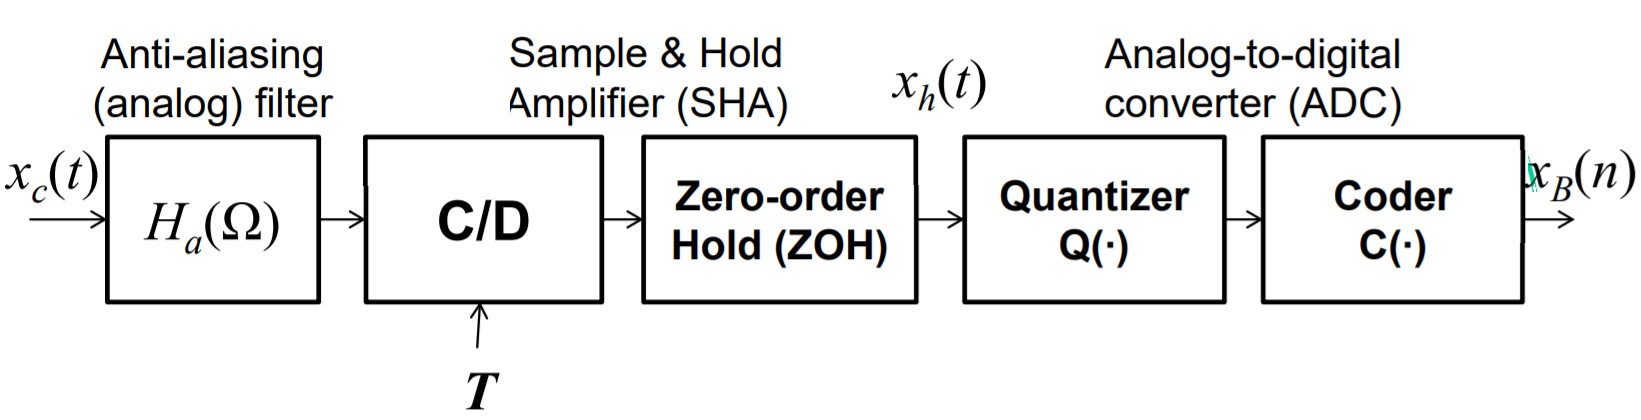
\includegraphics[width=10cm]{adc-steps}
			\caption{schematic representation of the steps used to perform an analog-to-digital conversion.} \label{fig:conv:adc}
		\end{figure}
		
		Considering the block diagram in figure \ref{fig:conv:adc}, to perform the analog-to-digital conversion the following steps are usually performed:
		\begin{enumerate}
			\item before doing the proper conversion, the analog signal is pre-processed in the analog domain by an anti-aliasing filter;
			\item with a sample\&hold amplifier the continuous time signal is discretized in the time domain (with a sampling time $T_s$) and is kept constant with a zero-order hold;
			\item the proper analog-to-digital conversion happens with the quantization (discretization in the signal domain) of the signal and it's consequence binary codification; usually this operations are performed at the same time.
		\end{enumerate}
				
		\subsection{Ideal filters} \label{sec:conv:filters}
			
			A \de{filter} is (typically) a linear system selective in the frequency domain that so determines which frequencies should be accepted and the one that should be removed.
			
			\begin{figure}[b]
				\centering 
				\begin{subfigure}{0.48\linewidth}
					\centering 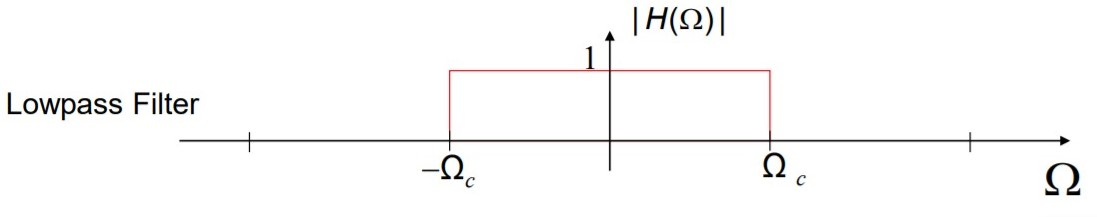
\includegraphics[width=\linewidth]{filter-low} \caption{}
				\end{subfigure} \\
				\begin{subfigure}{0.48\linewidth}
					\centering 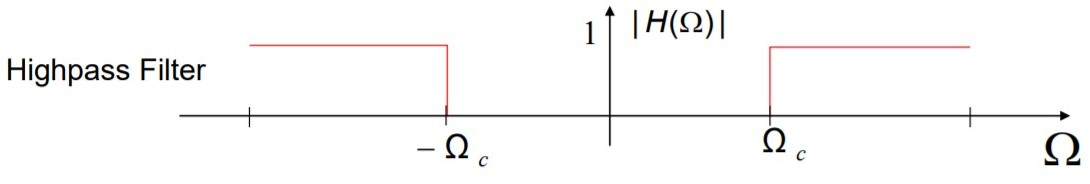
\includegraphics[width=\linewidth]{filter-high} \caption{}
				\end{subfigure}			
				\begin{subfigure}{0.48\linewidth}
					\centering 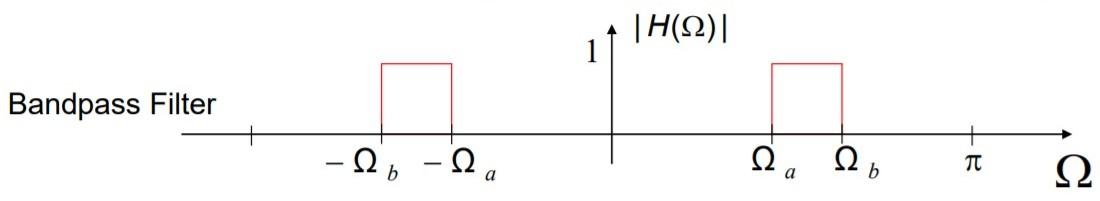
\includegraphics[width=\linewidth]{filter-band} \caption{}
				\end{subfigure}
				\caption{low-pass filter (a), high-pass filter (b) and band-pass filter (c) frequency response.} \label{fig:conv:idealfilters}
			\end{figure}
			
			As it can be seen in figure \ref{fig:conv:idealfilters}, the main types of ideal filters are the \textbf{low-pass} filter (accepting frequencies inside the range $[-\Omega_c,\Omega_c]$), the \textbf{high-pass} filter (removing frequencies in the range $[-\Omega_c,\Omega_c]$ and accepting the other ones) and the \textbf{band-pass} filter (accepting only a subset of the frequencies $[-\Omega_b,\Omega_a]$ and $[\Omega_a,\Omega_b]$); dual to such filter is the \textbf{stop-band} (not represented) that eliminates frequencies in the ranges $[-\Omega_b,\Omega_a]$ and $[\Omega_a,\Omega_b]$.
			
			Ideal filters cannot be implemented in real life because they are \textit{non-causal} systems  (focus on this definition will be stressed later on), meaning that in order to have such frequency behaviour we need to known also the future of the signal that we want to filter (and so that's impossible).			
		
		\subsection{Continuous-to-discrete time converter} \label{sec:conv:timeconversion}
			
			As previously discussed, the analog-to-digital conversion implies a \de{sampling} of the analog signal in order to transform it from continuous-time to discrete-time. Given in fact the continuous input signal $x_c(t)$ and the sampling period $T_s$, an ideal continuous-to-discrete conversion determines the following discrete-time sequence:
			\begin{equation}
				x(n) = x_c(nT_s) = x_c(t) \infsum n \delta(t-nT_s)
			\end{equation}
			
			Remembering that $\Omega$ is the analog frequency and that the related digital frequency is $\omega = \Omega T_s$, than expliciting the signal $p(t) = \infsum n \delta(t-nT_s)$ we can compute the frequency response of the digital signal as the convolution of the spectrum of the analog signal with the one generated by the train of pulses; using the windowing theorem (equation \ref{eq:four:windowing}, page \pageref{eq:four:windowing}) we indeed have
			\begin{equation}
				x(n) = x_c(t) p(t) \qquad \mapsto \qquad X(e^{j\omega}) = X_c(\Omega) * P(\Omega)
			\end{equation}
			Knowing that the transform $p(t)$ can be regarded as $P(\Omega) = \frac 1 {T_s} \infsum k \delta \left( \Omega - \frac{2\pi k}{T_s} \right)$ evaluating the convolution in the frequency domain determines the following spectrum:
			\begin{equation}
				X(e^{j\omega}) = \frac 1 {T_s} \infsum k X_c \left( \Omega - \frac{2\pi k}{T_s} \right) = \frac 1 {T_s} \infsum k X_c \left( \frac \omega {T_s} - \frac{2\pi k}{T_s} \right)
			\end{equation}
		
			As we can see from this expression, the digital spectrum resulting from the initial analog signal presents infinite \textbf{spectral replicas} that are a re-scalation by a factor $1/T_s$ distanced by a value $\frac{2\pi}{T_s}$ in the frequency axis from the original signal.
			
			\begin{figure}[b!]
				\centering 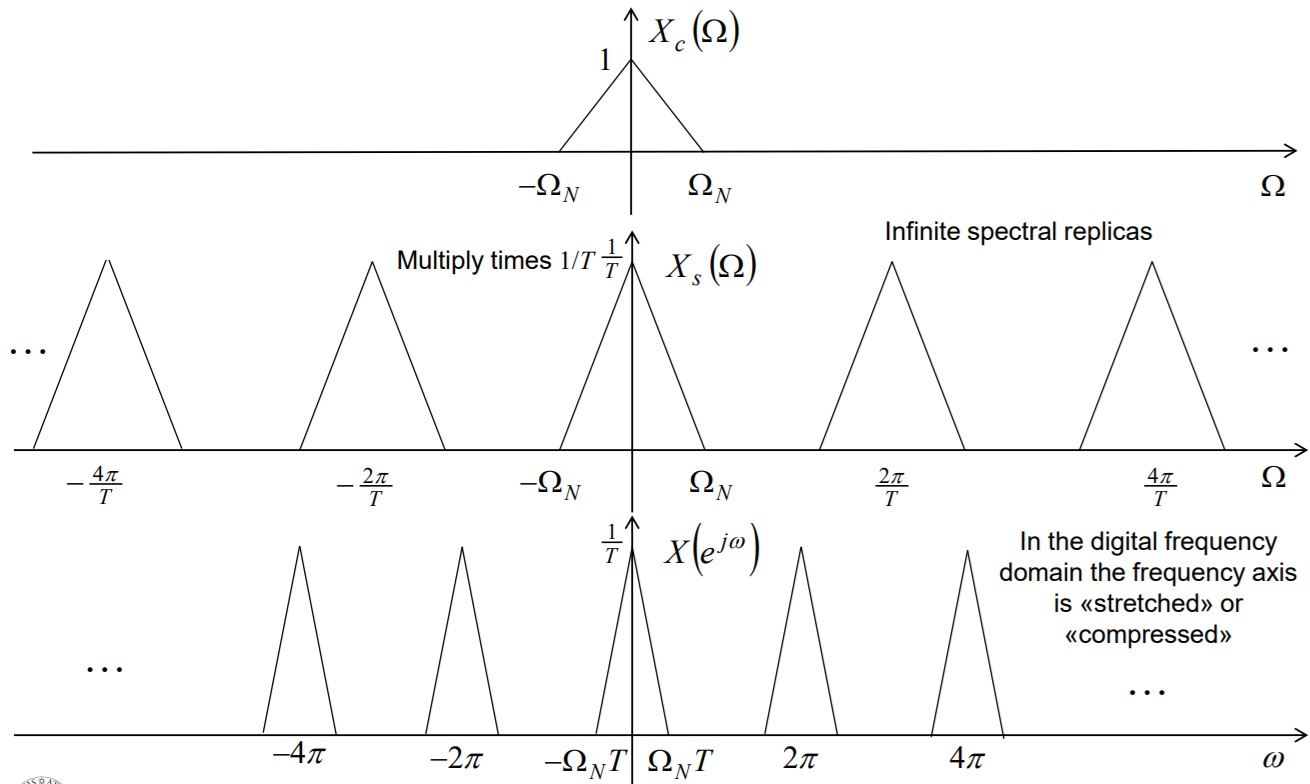
\includegraphics[width=13cm]{replicas}
				\caption{representation of the spectrum of the sampled signal.} \label{fig:conv:replicas}
			\end{figure}
			
			As shown in figure \ref{fig:conv:replicas}, to represent the spectrum $X(e^{j\omega})$ of the discretized signal knowing the original frequency response $X_c(\Omega)$ we have to perform the following steps:
			\begin{enumerate}
				\item build all the spectral replicas at distances $\Omega = \frac{2\pi}{T_s} k$ $\forall k \in \mathds Z$;
				\item multiply all the spectra by a coefficient $1/T_s$;
				\item remap the analog frequency variable $\Omega$ with the digital one $\omega$ using the relation $\omega = \Omega T_s$.
			\end{enumerate}			
		
		\subsection{Nyquist sampling theorem} \label{sec:conv:nyquist}
			
			The introduction of spectral replicas might lead to the problem of \de{aliasing} that happens every time the spectral replicas of the signal (due to the sampling) overlaps in the frequency domain, resulting in a distortion (in that region the frequencies adds up, altering the initial value); this problem arise every time the sampling period is too high (or reciprocally the sampling frequency is too low) respect to the characteristic value of the signal.
			
			The aliasing must always be avoided because the loss of information due to the overlaps of the replicas is irrecoverable and in order to to so it's mandatory to increase the sampling frequency (decrease the sampling period $T_s$) to avoid such overlap. Given $\Omega_n$ as the maximum frequency of the spectrum of the signal that we want to sample, than we have to ensure that
			\begin{equation}
				\Omega_n < \frac \pi {T_s}
			\end{equation}
			This inequality is the base of the \de{Nyquist-Shennon sampling theorem} that states that the maximum frequency of the signal to sample must be less than half of the sampling frequency; knowing that $f_n = \frac{\Omega_n}{2\pi}$ we have in fact that
			\begin{equation} \label{eq:conv:nyquist}
				2\pi f_n < \pi f_s \qquad \Rightarrow \qquad f_n < \frac{f_s}{2}
			\end{equation}
			ensuring so that $\omega_n < \pi$. We refer to the value $f_s/2$ as the \de{Nyquist frequency} and determines the upper bound o the allowable frequency of the input signal in order not to have aliasing. 
			
			The aliasing problem can so be avoided by designing a proper low-pass analog filter before the continuous-to-discrete time converter (in fact in figure \ref{fig:conv:adc} the filter was referred as \textit{anti-aliasing}).		
			
		\subsection{Sample \& hold}
			
			After the time-discretization process has happened, the output passes through a \textbf{Zero-Order Hold} filter that sets as constant the output with a value equal to the input and resets each period $T_s$; this time is in particular chosen in order to allow the ADC block to perform it's conversion operations. Such filter should also avoid the problem of the \textit{shocking} of the transients due to the switch commutations.
			
		
			From a practical point of view the time discretization and the zero-order hold is performed by the \de{sample \& hold amplifier} whose electronic circuit is shown in figure \ref{fig:conv:samplehold}.		
			This kind of circuit implementation resamples a low pass electrical filter; ideally while the sampling signal $v_c$ is set to high, the output $v_y$ is set equal to the input voltage $v_x$ while when $v_c$ is low the exit remains constant (hold operation) due to the ideally constant charge of the capacitor whose also charge time has considered negligible.
			
			Real implementations have to consider both the charge time of the capacitor $C_H$ as well as the fact that the component discharges with time due to parasitic currents; from a design point of view lower capacitances $C_H$ decreases the time required for the charge with the drawback of also increasing the effect of the current leak and so there's always a trade-off between this aspects.
		
			\begin{figure}[bh]
				\centering
				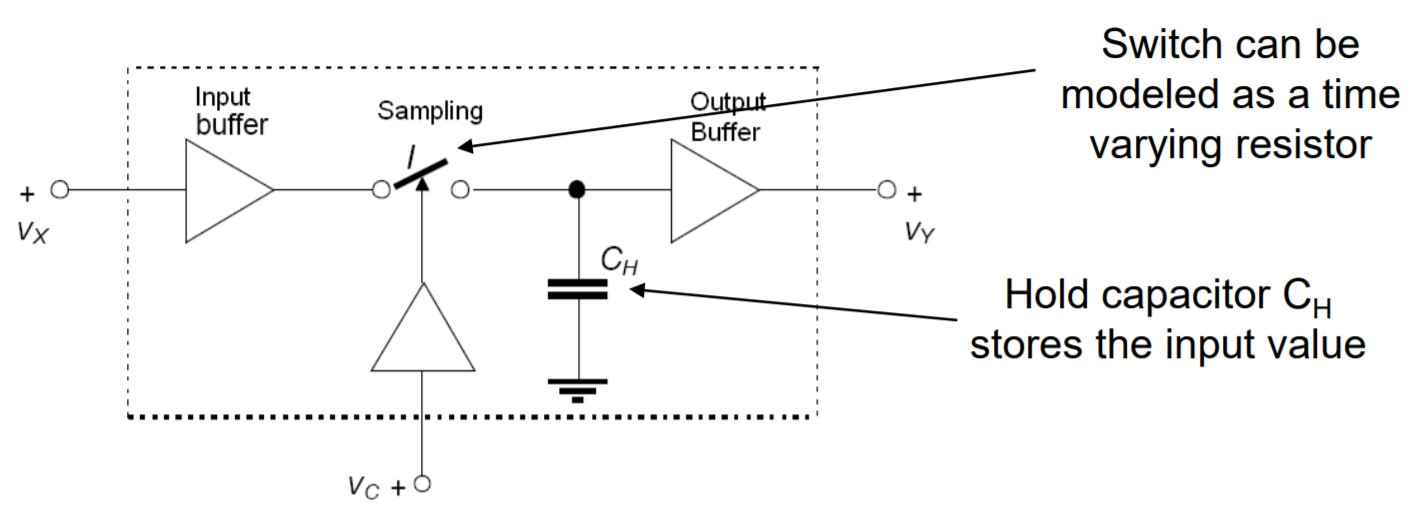
\includegraphics[width = 11cm]{samplehold}
				\caption{possible implementation of an electrical sample \& hold amplifier. }
				\label{fig:conv:samplehold}
			\end{figure}
		\subsection{Quantization and codification}
			
			With a sample \& hold amplifier we have a signal that's constant in the sampling period $T_s$, the next step is to perform the proper analog-to-digital conversion that consists in the operations of \de{quantization} (discretization of the values) and the consequent \de{codification} in binary representation.
			
			\paragraph{Quantization} To quantization action is performed on a pre-defined range (usually on voltages) $[V_{min}, V_{max}]$ that's subdivided into disjoint intervals $I_k = (T_{k-1},T_k]$ where $T_k$ is the $k$-th threshold voltage. Each interval so corresponds to a certain code bin $Q_k$ that's $T_{k}-T_{k-1}$ wide. An ideal analog-to-digital converter has the characteristic that
			\[ Q(x_s) = Q_k \qquad \text{for } T_{k-1} < x_s \leq T_k \]
			By graphically representing this function (figure \ref{fig:conv:quantization}) we can see it \textit{stair-case response} that determines the \textbf{quantization levels} of the quantized.
			
			\begin{SCfigure}[2][bht]
				\centering
				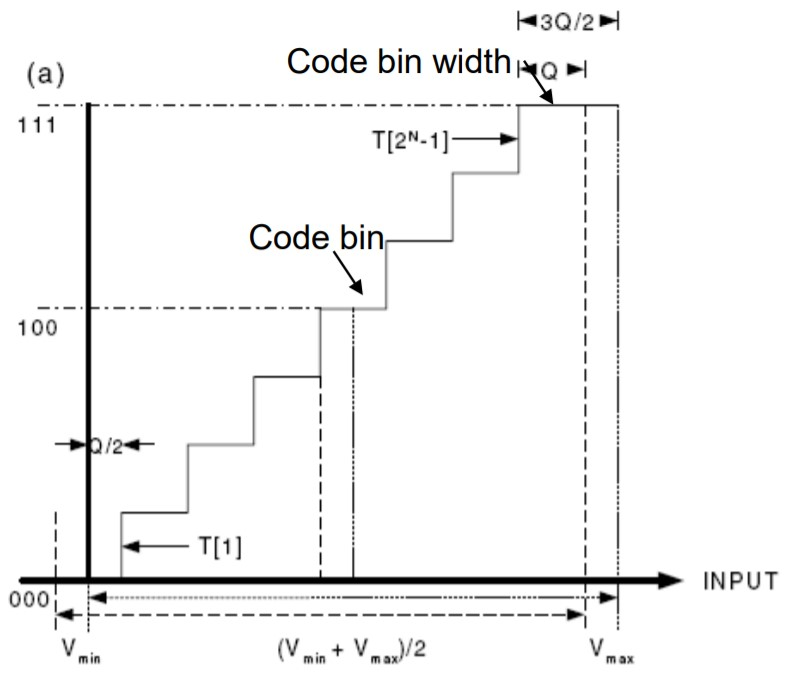
\includegraphics[width=6cm]{quantization}
				\caption{graphical representation of the stair-case function that determine the quantization of a signal.} \label{fig:conv:quantization}
			\end{SCfigure} 
			
			\noindent
			Depending on the possible value of the inputs, ADCs can be classified as
			\begin{itemize}
				\item unipolar if $V_{min} = 0$ and $V_{max} = F_s$;
				\item bipolar if $V_{min} = - F_s$ and $V_{max} = F_s$.
			\end{itemize}
			The number of quantization levels is of course related to the digital implementation of the system: given $b$ the number of bits that the ADC block can output, then the maximum number of allowed bins are $2^b$ with $2^b-1$ quantization thresholds. Assuming to have quantization steps with equal length $\Delta$, then such value can be computed as
			\begin{equation}
				\Delta = \begin{cases}
					\frac{2F_s}{2^b} = \frac{F_s}{2^{b-1}} \qquad & \text{bipolar case} \\
					\frac{F_s}{2^b} \qquad & \text{unipolar case} \\
				\end{cases}
			\end{equation}
			and so increasing the number of bits, the resolution improves exponentially.
			
			\paragraph{Error analysis} As the quantization operation is a non-linear operation a fully analytical model is complex, however if the input signal changes randomly and the difference between two consecutive samples is much larger than the quantization step, the error can be modelled as a realization of additive stochastic processes $e_q(\cdot)$ that can be regarded as
			\begin{itemize}
				\item white and stationary;
				\item uncorrelated to the input signal $x_s$;
				\item with a uniform probability density function.
			\end{itemize} 
			The quantization operation can work with a rounding on the value and the range of uniformity of the PDF is $[-Q/2,Q/2]$ (as shown in figure \ref{fig:conv:quantizationerror}) while if we use a truncation model then the range is shifted becoming $[-Q,0]$. In both case the mean and the variance of the quantization noise is
			\begin{align*}
				\mu_q & = 0 \qquad & \sigma_q^2 & = \frac{Q^2}{12} \qquad && \text{rounding case} \\
				\mu_q & = -\frac Q2 \qquad & \sigma_q^2 & = \frac{Q^2}{12} \qquad && \text{truncation case}
			\end{align*}
		
			\begin{SCfigure}[2][bht]
				\centering
				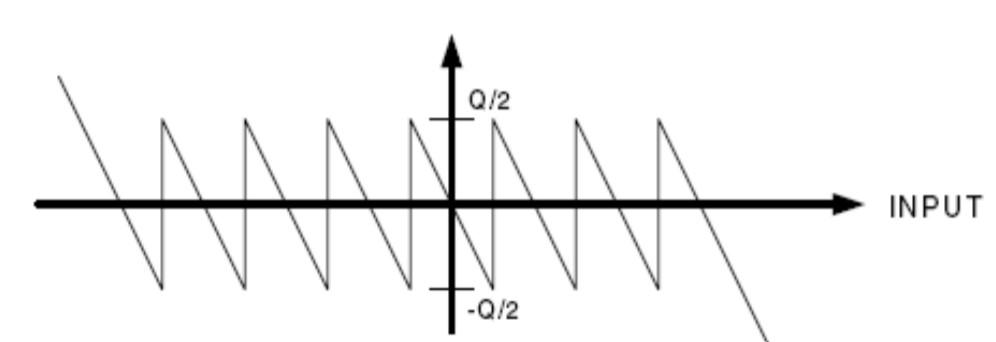
\includegraphics[width=6cm]{quanterror}
				\caption{quantization error due to a rounding quantization.} \label{fig:conv:quantizationerror}
			\end{SCfigure}
			
			\paragraph{Signal-to-noise and quantization ratio} The \textbf{signal-to-noise and quantization ratio} $SQNR$, usually expressed in decibels, is a parameter that allows to compare the variance of the quantization error respect to the one of the original signal:
			\begin{equation}
				SQNR := \frac{\sigma_x^2}{\sigma_q^2}
			\end{equation}
			
			Considering the case of a rounding quantization error, the $SQNR$ parameter in decibel can be expressed as
			\begin{equation}
			\begin{aligned}
				SQNR_{dB} & = 10 \log_10\left(\frac{\sigma_x^2}{\sigma_q^2}\right) = 10 \log_{10} \left( \sigma_x^2 \frac 3 {F_s^2} 2^{2b} \right) \\ \Rightarrow \quad SQNR_{dB}  & \approx 6.02b + 20\log_{10}\sigma_x + 20\log_{10} \left( \frac{\sqrt 3}{F_s} \right)
			\end{aligned}
			\end{equation}
			This means that for each bit $b$ added on the quantization level, the potential improvement of the signal-to-noise ratio is of about $6dB$; in general a good rule to design the number of bits to have a low quantization error is
			\begin{equation}
				b = \frac 1 2 \log_2 \left( \frac{\sigma_x^2}{\sigma_q^2} \right)
			\end{equation}
			
			A more accurate description of the analog-to-digital converter performance might take into account other imperfection; considering the original signal $\hat x$
			\[ \hat x(n) = x(n) + e_q(n) + e_\omega(n) \]
			described as the sum of the quantized signal $x$, the quantization error $e_q$and other external noises $e_\omega$ then we can compute the \textbf{signal-to-noise ration} $SNR$ as
			\begin{equation}
				SNR = \log_2 \left( \frac{\sigma_x^2}{\sigma_e^2 + \sigma_\omega^2} \right) < SQNR
			\end{equation}
			This expression has been obtained considering all error as uncorrelated (modelled as white noises) with a more gaussian than normal distribution.
			
			\paragraph{ENOB} In the assumption of having statistically independent noise sources $e_q,e_\omega$, then it's possible to compute the \de{effective number of bits} $ENOB$ as
			\begin{equation}
				ENOB = \frac 1 2 \log_2 \frac{\sigma_x^2}{\sigma_q^2 + \sigma_\omega^2}
			\end{equation}
			Considering so the case of an ADC constructed with a $16bit$ quantization, if the $ENOB$ is lower, like $12bit$ then the last $4$ significant bits are \textit{meaningless} because they are affected by the ADC noises.
						
		\subsection{Technology implementations}
			
			In general analog-to-digital converters are classified in categories depending on their technology implementation that allows to achieve particular performances in terms of number of bits and sampling frequencies. As general behaviour, higher resolution (number of bits) requires lower sample rate while if the number of samples per second required is high, the resolution inevitably drops. As a rule of thumb, decreasing the nominal resolution by a bit determined a double sampling frequency.
			
			\begin{SCfigure}[1][bht]
				\centering
				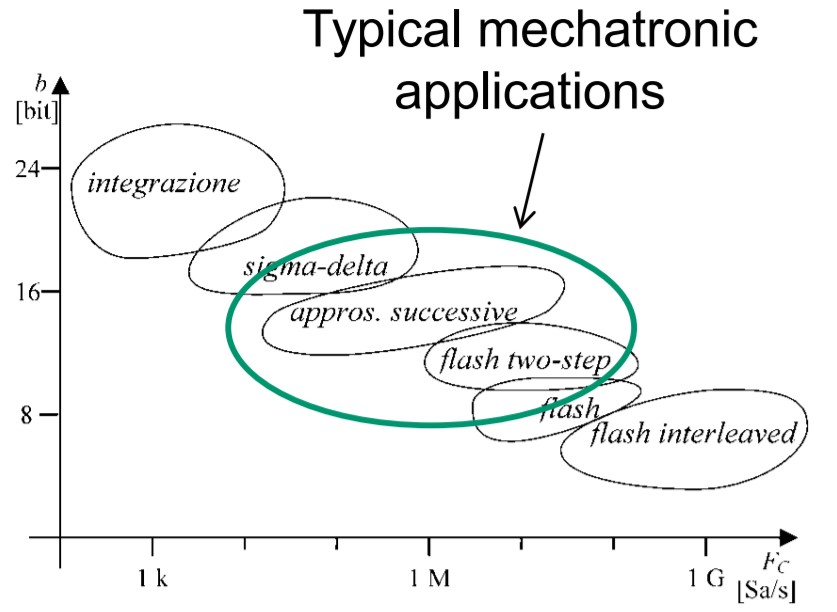
\includegraphics[width=6.5cm]{adc-families}
				\caption{families of analog to digital converters with associated performance as sample per second ($x$ axis) and resolution bits ($y$ axis).}
			\end{SCfigure}
		
			For mechatronics applications usually successive-approximation ADC's (or ones with similar properties) are chosen for having the best trade-off between frequency and resolution.			

\section{Digital-to-analog converter}
	
	A \de{digital-to-analog converter} \textbf{DAC} is a component whose scope is to reconstruct a continuous-time analog signal from a discrete-time digital value.
	
	Given the discrete-time input sequence $y(n)$ that has to be transformed in the continuous-time signal $y_c(\cdot)$, the reconstruction can happens simply considering an ideal \textbf{low-pass reconstruction filter} with gain $T_s$ and cut-off frequency of $\pi/T_s$. From a spectral point of view the obtained result is
	\begin{equation}
		Y_c(\Omega) = T_s \, Y\big(e^{j\Omega T_s}\big) \qquad \textrm{for } |\Omega| \leq \frac \pi {T_s}
	\end{equation}
	Intuitively the gain of $T_s$ is due to the fact that, in the analog-to-digital conversion, the spectra was attenuated by a multiplicative factor $1/T_s$ and so the low-pass reconstructor filter must \textit{compensate} for such error; the filter should also be low-pass in order to avoid the propagation of the spectral replicas of the sampled signal.
	
	\begin{figure}[bht]
		\centering 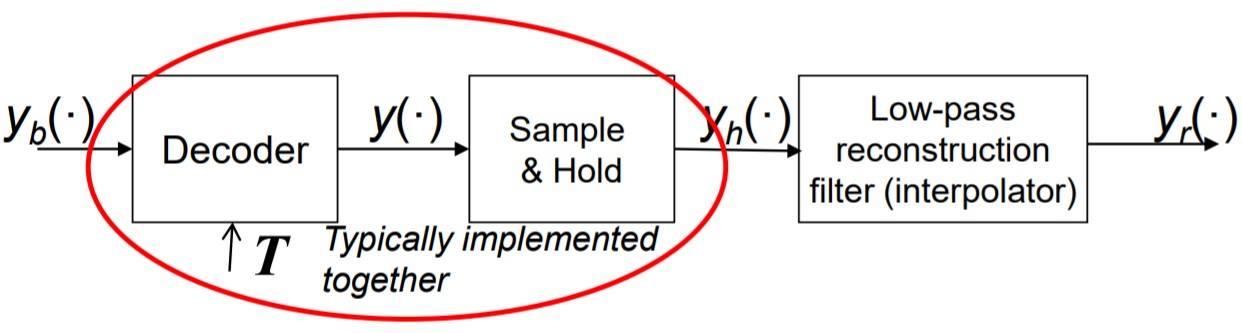
\includegraphics[width=10cm]{DAC-scheme}
		\caption{schematic  representation of the steps/components used to perform a digital-to-analog conversion.} \label{fig:conv:DACscheme}
	\end{figure}
	
	\paragraph{Real DAC considerations} Considering a real implementation of a digital-to-analog converter, as shown in figure \ref{fig:conv:DACscheme}, 3 main steps must be performed:
	\begin{enumerate}
		\item decodification of the digital value into (generally) an analog voltage; such operation is performed by a \textbf{decoder};
		\item after the decoding, a \textbf{sample \& hold} operation must take place for a sampling period $T_s$: this allows to re-introduce the concept of \textit{time} that in the digital domain was lost. Usually this component is automatically embedded in the decoder implementation;
		\item lastly a \textbf{low-pass reconstructor filter}, also called \textbf{\textit{interpolator}}, is used to avoid replicas and to \textit{smoothen} the output.
	\end{enumerate}
	
	Considering the schematic representation of figure \ref{fig:conv:DACscheme}, the signal $y_h(t)$ resulting from the sample \& hold operation is a staircase function that can be described as
	\begin{align*}
		y_h(t) & = \infsum n y(n) \rect_{T_s} \left( t - \frac{T_s}2 - nT_s \right) = \infsum n y_c (nT_s) \rect_{T_s}\left( t - \frac {T_s} 2 - nT_s \right) \\
		& = y_c(t) \left[ \rect_{T_s} \left( t - \frac{T_s}{2} \right) * \infsum n \delta(t-nT_s) \right]
	\end{align*}
	Using the properties of the \ctft (in particular the convolution and the windowing theorem), then the spectra of the signal $y_h$ can be regarded as
	\begin{equation}
	\begin{aligned}
		Y_h(\Omega) & = Y_c(\Omega) * \left[ T_s \sin\left(\frac{\Omega T_s}{2}\right) e^{-j\Omega \frac{T_s}{2}}  \frac 1 {T_s} \infsum k \delta\left( \Omega - \frac{2\pi k}{T_s} \right) \right] \\
		& = Y(\Omega) T_s \sinc \left(\frac{\Omega T_s}{2}\right) e^{-j\Omega \frac{T_s}2}
	\end{aligned}
	\end{equation}
	From this expression we can see that the spectrum resulting from the zero-order-hold is a modified (by a $\sinc$ function) frequency response from $Y(\Omega)$ generated by the decoder. The ideal implementation of the reconstructor filter $\hat H_r$ is so to compensate the non-ideal behaviours introduced by the zero-order-hold and so
	\begin{equation}
		\hat H_r = \begin{cases}
			\frac{T_s}{H_h(\Omega)} \qquad & |\Omega|\leq\frac{\pi}{T_s} \\ 0 & \textrm{otherwise}
		\end{cases}
	\end{equation}
	
	
	
\section{Multi-rate signal processing}
	
	Until now we consider conversions with a defined sampling frequency $f_s = 1 / T_s$, however sometimes it might be necessary to increase or decrease such value to perform better analysis; in particular frequency should be increase if the processor cannot \textit{keep up in speed} with the real-time processing, while increasing speed might be good to have a better read-out in the time domain.
	
	In general we refer as \de{multi-rate signal processing} the operation that allows, starting from a fixed sampling frequency $f_s$, to decrease (\textbf{undersampling} case) or increase (\textbf{upsampling}) the number of samples per second.

	\subsection{Undersampling}
		
		The \de{undersampling} operation, referred also as \textbf{decimation}, is an operation that decreases the sampling rate by a so called \textbf{decimation factor} $M$ (that's an integer value). The \de{compressor} (figure \ref{fig:conv:compressor}) is the \textit{block} that so performs the undersampling operation by selecting $1$ over $M$ samples. Mathematically, given the \textit{full} input discrete-time sequence $x(n)$, the compressor determines a new sequence
		\begin{equation}
			x_d(n) = x(nM) \hspace{2cm} M \in \mathds N
		\end{equation}
		
		\begin{SCfigure}[2][bht]
			\centering 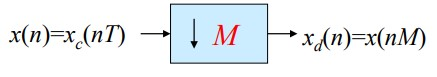
\includegraphics[width=6cm]{compressor}
			\caption{compressor performing an undersampling with decimation factor $M$.} \label{fig:conv:compressor}
		\end{SCfigure}
		
		Determined $T_s' = M T_s$ the new \textit{decimated} sampling period, we can describe the impact of this operation by analysing the spectral changes in the output of the system:
		\begin{equation}
		\begin{aligned}
			X_d\big(e^{j\Omega T_s'}\big) & = \frac 1{MT_s} \infsum k X_c\left( \Omega - \frac{2\pi k}{MT_s} \right)  = \frac 1{T_s'} \infsum k X_c\left( \Omega - \frac{2\pi k}{T_s'} \right)  \\
			X_d(e^{j\omega}) & = \frac 1 {T_s'} \infsum k X_c\left( \frac{\omega}{T_s'} - \frac{2\pi k}{T_s'}\right)
		\end{aligned}
		\end{equation}
		From this expression we can see that the main draw-back of undersampling is that it narrows the distance of the spectral replicas that in the discrete frequencies domain $\omega$ correspond to a shrink of a factor $1/M$, as shown in figure \ref{fig:conv:undersamplingresults}. The loss of information due to a lower sampling frequency is caused by the aliasing, and so to avoid such problem we have to be sure that
		\[ X_c\big( e^{j\omega} \big) = 0 \hspace{2cm} \textrm{for } |\omega|\geq \frac \pi M \]
 		This assertion can be ensured by pre-processing the input sequence $x_c(n)$ with a low-pass filter with unitary gain and cut-off frequency of $\pi/M$.
 		
 		\begin{SCfigure}[2][bht]
 			\centering 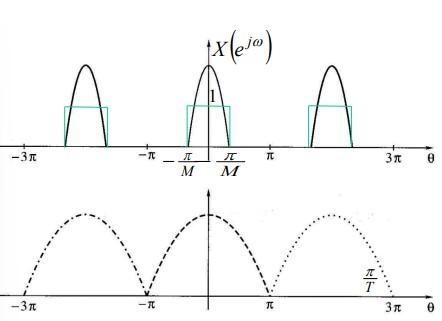
\includegraphics[width=6cm]{downsampling}
 			\caption{original spectra $X_c(e^{j\omega})$ and it modification after a decimation with $M=2$.} \label{fig:conv:undersamplingresults}
 		\end{SCfigure}	
	
	\subsection{Upsampling}
		
		The goal of \de{upsampling}, also referred as \textbf{interpolation}, is increasing the sampling frequency by decreasing the sampling period by a \textbf{interpolation factor} $L$:
		\[ T_s' = \frac{T_s}{L} \hspace{2cm} L \in \mathds N \]
		
		\begin{SCfigure}[2][bt]
			\centering 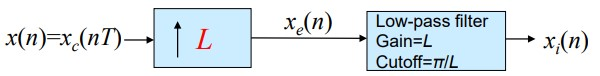
\includegraphics[width=0.5\linewidth]{upsampling}
			\caption{interpolation scheme with an expander and a interpolator block.}
			\label{fig:conv:upsamplingscheme}
		\end{SCfigure}
	
		This operation, performed by the \de{expander} (figure \ref{fig:conv:upsamplingscheme}), add new samples in the sequence by adding $L-1$ zeros after each sample, determining the expanded sequence defined as
		\begin{equation}
		x_e(n) = \begin{cases}
			x(n/L) \qquad & n = 0,\pm L, \pm 2 L,\pm 3L \dots \\
			0 & \textrm{otherwise}
		\end{cases}
		\end{equation}		
		
		Upon this sequence we can calculate it's \dtft resulting in 
		\begin{equation}
		\begin{aligned}
			X_e\big(e^{j\omega}\big) & = \infsum n x_e(n) e^{-j\omega n} = \infsum k x(k) e^{-j\omega kL} = X\big(e^{j\omega'}\big) \\
			& = \frac 1{T_s} \infsum k X_c\left( \frac{\omega'}{T_s} - \frac{2\pi k}{T_s} \right) = \frac 1{LT_s'} \infsum k X_c\left( \frac{\omega}{T_s'} - \frac{2\pi k}{LT_s'} \right)
		\end{aligned}
		\end{equation}
		where $\omega' = \omega L$. From a graphical point of view (figure \ref{fig:conv:upsampling}) this expression shrinks the original replicas by a factor $L$ (multiplication by $1/L$) and adds new replicas every $T_s/L$; the magnitude has also been reduced by a factor $L$. In order so to remove the new images created and \textit{resize} the spectrum a discrete-time interpolating low-pass filter with gain $L$ and cut-off frequency $\pi/L$ is required.
		
		\begin{SCfigure}[2][bht]
			\centering 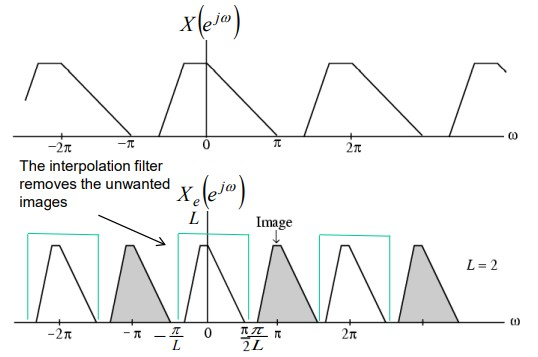
\includegraphics[width=0.5\linewidth]{upsampling-graph}
			\caption{original spectrum due to the sampling of a signal (upper) and upsampled spectrum (bottom) of the same signal with a value $L=2$.}
			\label{fig:conv:upsampling}
		\end{SCfigure}
		
		
		
		
		
		
		
		
	
	
	
	
	
	
	
	
	
	
	
	
	
	
	
	
	
	
	
	
	
	
	
	
	
	
	
	
	
	
	
	
	\chapter{Discrete/Fast Fourier Transform and Spectral Estimation}
\section{Discrete Fourier transform}
	
	As was discussed in chapter \ref{sec:fourietransforms}, the \dtft is an operator that allows to describe a discrete-time signal in the domain of the frequencies $\omega$. From a formal point of view the definition is clear and straightforward, but still is impractical for numerical calculations.
	
	For this reason the \de{Discrete Fourier Transform} \textbf{DFT}, usually expressed as $X(k)$, has been created and can be regarded as the \textbf{discretization} in the \textbf{frequency domain} of the DTFT spectrum $X(e^{j\omega})$. Considering in fact that such spectra is the continuous evaluation of the Z transform around the unit complex circle (by changing $\omega$ in the domain $[0,2\omega]$ in the function $e^{j\omega}$), by choosing $N$ samples of angle $\omega_k[rad]$ with $k=0,\dots,N-1$ we obtain the discretized spectra function of $k$ as
	\begin{equation} \label{eq:dft:dft}
		X(k) = \sum_{n=0}^{N-1} x(n) e^{-j\frac{2\pi}Nkn} = \sum_{n=0}^{N-1} x(n) W_{N}^{kn} \hspace{2cm} \forall k = 0,\dots, N-1
	\end{equation}
	where the term $W_N = e^{-j\frac{2\pi}{N}}$ is usually referred as \textit{\textbf{twiddle factor}}.
	\begin{SCfigure}[2][bht]
		\centering 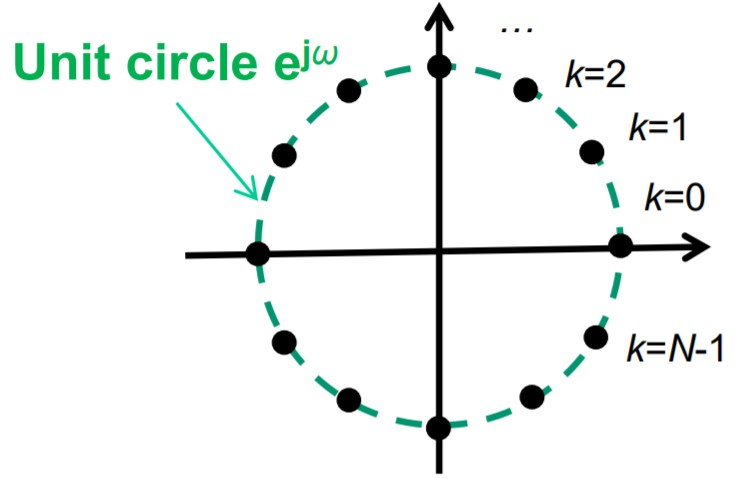
\includegraphics[width=5cm]{unit-circle}
		\caption{point on the Z plane on which the DFT is evaluated in order to have a \dft.} \label{fig:dft:unitcircle}
	\end{SCfigure}
	
	Intuitively, as can be deduced from figure \ref{fig:dft:unitcircle}, increasing the number of samples $N$ in the unit circle means decreasing the \textit{distance} between each angle $\omega_k$ and so for $N\rightarrow \infty$ the DFT computation converges to the DTFT.\\
	Note that the \dft is not an approximated version of the DTFT: in fact evaluating both function for the same angle $\omega_k$ will result in equal results, but the DFT is just a pure sampling of the DTFT in the frequency domain.
	
	\paragraph{Evaluation of the DFT} The \dft is so a better numerical formulation (in a sense that can be algorithmically implemented for automatic computation) that allows to estimate the spectra of a discrete-time signal. Even if the formulation in equation \ref{eq:dft:dft} can be automatized, the numerical cost complexity is quite high: better performance can be obtained by using the so called \de{Fast Fourier Transforms} \textbf{FFT} (better described lates), a set of complementary algorithms that aims at improving computational performance while still not impacting the final result.
	
	\paragraph{Inverse DFT} As for the Fourier transform, it's possible to define a \de{Inverse Discrete Fourier Transform}	 IDFT, an operator that allows to reconstruct a signal $x(n)$ from it's DFT $X(k)$:
	\begin{equation} \label{eq:dft:inversion}
		x(n) = \frac 1 N \sum_{n=0}^{N-1} X(k) e^{j\frac{2\pi}{N} kn } \hspace{2cm} \forall n = 0,\dots, N-1
	\end{equation}
	Such operation is the pure inversion of the DFT expression stated in equation \ref{eq:dft:dft}. We can in fact see that the spectrum can be computed as a linear combination of the the twiddle factors, in fact equation \ref{eq:dft:dft} can be expresses in a matrix form as
	\[ \underbrace{\begin{pmatrix}
		X(1) \\ X(2) \\ \vdots \\ X(N-1)
	\end{pmatrix}}_{\underline X} =  \underbrace{\begin{bmatrix}
		W_N^{1\cdot 1} & W_N^{1\cdot 2} & \dots & W_N^{1(N-1)} \\
		W_N^{2\cdot 1} & W_N^{2\cdot 2} & \dots & W_N^{2(N-1)} \\
		\vdots & \vdots & \ddots \\		
		W_N^{(N-1) 1} & W_N^{(N-1)\cdot 2} &  & W_N^{(N-1)(N-1)} \\
	\end{bmatrix}}_W \underbrace{\begin{pmatrix}
		x(1) \\ x(2) \\ \vdots \\ x(N-1)
	\end{pmatrix}}_{\underline x} \]
	Having the linear system $\underline X = W \underline x$, it's inversion $\underline x = W^{-1} \underline X$ is in fact the pure definition of the inverse \dft in equation \ref{eq:dft:inversion}.
	
	\subsection{Time aliasing}
		Given a discrete-time signal $x(n)$ with $L$ samples, meaning that
		\[ x(n)  \begin{cases}
			\neq 0 \qquad & n = 0,\dots, L-1 \\ = 0 & \textrm{otherwise}
		\end{cases} \]
		resulting  in a DTFT $X(e^{j\omega})$, the related \dft $X(k)$ can  be computed over a number of frequency discretization $N$ that's not necessary equal to $L$ (however this might sound the most common selection).
		
		Depending on the number of frequency discretization $N$ the application of the inverse \dft (equation \ref{eq:dft:inversion}) might lead to a reconstructed signal $\hat x(n)$ that's not necessary equal to the original sequence $x(n)$. By applying the definition in fact we have
		\begin{equation} \label{eq:dft:timealiasing}
		\begin{aligned}
			\hat x(n) & = \frac 1 L \sum_{k=0}^{L-1} \left( \sum_{m=0}^{N-1} x(m) e^{-j \frac{2\pi}{N}km} \right) e^{j\frac{2\pi}{L} kn} \\
			& = x(n) * \infsum r \delta(n-rN) = \infsum r x(n-rN)
		\end{aligned}
		\end{equation}
		From this result (obtained by computing the DTFT assuming $N\rightarrow \infty$ and after some algebraic manipulation) we can observe that
		\begin{itemize}
			\item if $N\geq L$ then the reconstructed signal $\hat x(n)$ is equal to the original signal $x(n)$;
			\item if $N < L$ then the reconstructed signal $\hat x(n)$ differs from the original $x(n)$.
		\end{itemize}
		
		The difference is due to the phenomena of the so called \de{\textit{time aliasing}} (shown in figure \ref{fig:dft:timealiasing}): from expression \ref{eq:dft:timealiasing} we can see that the IDFT computes a periodic signal with periodicity $N$ and so if $N < L$ then the last (and so the first) $L-N$ samples \textit{cyclically adds-up} by generating the phenomena of the time aliasing.		
		
		\begin{SCfigure}[2][bht]
			\centering 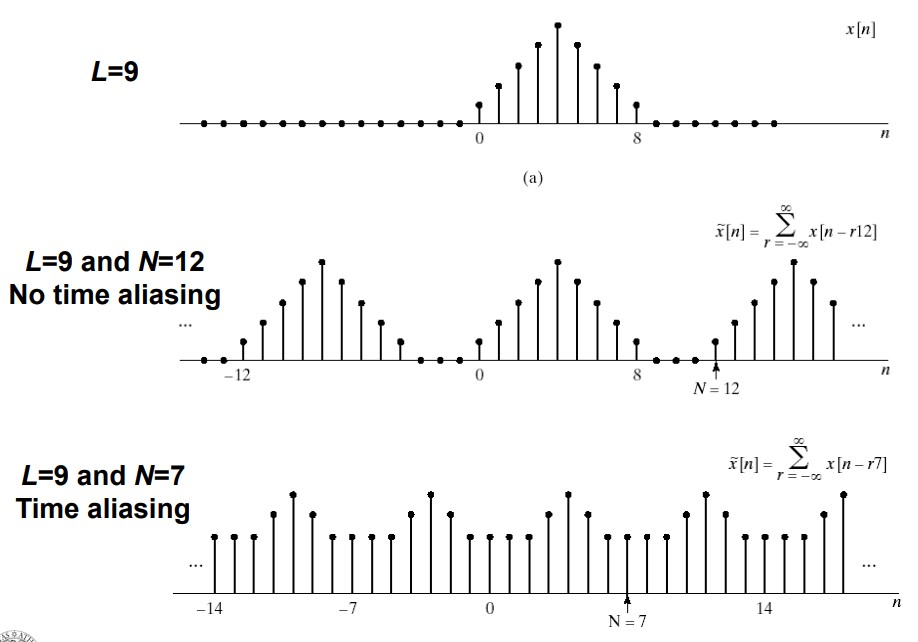
\includegraphics[width=8.5cm]{time-aliasing}
			\caption{ on top: original sequence $x(n)$ consisting of $L=9$ samples; below DFT+IDFT computed on $N = 12 (>L)$ and $N = 7(< L)$ samples; in the second case we can observe the phenomena of the time aliasing. } \label{fig:dft:timealiasing}
		\end{SCfigure}
		
		As was discussed at page \pageref{sec:conv:nyquist}, a sampling in the time domain can result in aliasing in frequency domain and so, dually, a sampling in the frequency domain results in time aliasing. The dual condition to the Nyquist frequency (eq. \ref{eq:conv:nyquist}, page \pageref{eq:conv:nyquist}) is so having 
		\begin{equation}
			N\geq L
		\end{equation}
	
	\subsection{Properties}
		
		The \dft is still a \textbf{linear operator}: given two discrete-time signals $x_1(n),x_2(n)$ having DFT's $X_1(k), X_2(k)$ then
		\begin{equation}
			ax_1(n) + b x_2(n) \qquad \mapsto \qquad aX_1(k) + bX_2(k) \hspace{2cm} \forall a,b \in \mathds R
		\end{equation}
		If this two sequences are characterized by different length $L_1,L_2$ (and as example we assume $L_2>L_1$), in order to apply such property is mandatory to perform the so called \de{\textit{zero padding}} that consist on adding $|L_1-L_2|$ zeros at the and of the shortest sequence (in this case the second) and then computing the DFT on $N = L_1 = L_2 + |L_1-L_2|$ (or on a higher \textit{sampling in the frequency domain}).
		
		\paragraph{Circular shifting} Given a sequence $x(n)$ of $L$ samples with associated \dft $X(k)$, then given an integer time shift of $m\in \mathds Z$ samples determines
		\begin{equation}
			\tilde x(n-m) \quad \textrm{with } n =0,\dots, N-1 \hspace{1.2cm} \mapsto \qquad X(k) e^{-j\frac{2\pi k}{L}m}
		\end{equation} 
		where $\tilde x(n)$ is the \textit{infinite repetition} of the signal $x(n)$ obtained by it's iterative concatenation.
		
		\paragraph{Symmetries} As for the Fourier transform, if the discrete-time signal $x(n)$ is real evaluated, then the DFT (with a frequency sampling of $N$ samples) of such signal presents an even symmetry on the real axis, and in particular we obtain
		\begin{equation}
			\Re{X(k)} = \Re{X(N-k)} \hspace{2cm} \Im{X(k)} = - \Im{X(N-k)}
		\end{equation}
		
		\paragraph{Convolution and circular convolution} Given two discrete-time signals $x_1(n),x_2(n)$ having each length $L,P$ and DFT $X_1(k),X_2(k)$, then the \textit{linear} convolution property still holds:
		\begin{equation}
			x_3(n) = x_1(n) * x_2(n) \qquad \mapsto \qquad X_3(k) = X_1(k) X_2(k)
		\end{equation}
		With this definition, by computing the inverse \dft we retrieve a periodic signal $ \tilde x_3(n) = \tilde x_1(n) * x_2(n) = x_1(n) * \tilde x_2(n)$ that differs from the expected $x_3(n)$.\\
		Considering instead a convolution performed over $N$ samples, then such signal is referred as \de{circular convolution} defined as
		\begin{equation}
			x_1(n) \circconv N x_2(n) := \sum_{m=0}^{N-1} x_1(m) \tilde x_2(n-m)
		\end{equation}
		In order to perform a proper \dft that holds $x_1(n)*x_2(n) = x_1(n) \circconv N x_2(n)$ we must ensure that the DFT is computed over a set of frequency sample $N \geq L+ P - 1$; if this condition isn't met, then linear and circular convolution results are different.
		
		\paragraph{Impulse response} As was described in section \ref{sec:conv:impulseresponse} (page \pageref{sec:conv:impulseresponse}), we denote as $h(n)$ the impulse response of a discrete-time system and in the case it present a finite impulse response (FIR system) with $P$ non-zero samples, so such that
		\[ h(n) \neq 0 \qquad \textrm{for } n = 0,\dots, P-1 \]
		Assuming to have an input $x(n)$ made of $L$ non-zero samples, then the output $y(n)$ of the system can be described by the linear convolution (that has a maximum of $L+P-1$ non-zero samples):
		\[ y(n) = x(n) * h(n) \neq 0 \qquad \textrm{for } n=0,1,\dots, L+P-2 \]
		
		Solving this problem in the frequency domain using the \dtft, known the transforms $X(e^{j\omega}), H(e^{j\omega})$  we obtain the frequency response as multiplication of this two spectrum:
		\[ Y(e^{j\omega}) = X(e^{j\omega}) H(e^{j\omega}) \qquad \xrightarrow{\F^{-1}} \qquad y(n) \]
		
		Knowing that the analytical solution is not practical from a numerical point of view, we have to use the \dft that can algorithmically implemented. Known the discrete transforms $X(k),H(k)$ made by $L,P$ samples each, then in order to perform a proper convolution operation we have to set both initial signals $x(n),h(n)$ to a length $N=L+P-1$ (by so performing a zero-padding of $P-1$ samples on $x(n)$ and of $L-1$ samples on $h(n)$): after this operation we are sure that the DFT product $X(n)H(n)$ has a number of samples $N = L+P \geq L+P-1$ that allows to have a proper linear convolution without time aliasing.		
		
\section{Fast Fourier transforms}
	
	\de{Fast Fourier Transforms} \textbf{FFT}s are a class of algorithms used to compute \textit{in a faster way} (by decreasing the numerical computational complexity) of the \dft by using some \textit{mathematical tricks} that are gonna shown later.
	
	\paragraph{Computational cost} Considering the formal definition of the DFT state on page \pageref{eq:dft:dft} (equation \ref{eq:dft:dft}) we can see that the computation of a spectrum with $N$ samples in the frequency domain involves $N-1$ complex additions and $N$ complex multiplications for each spectral sample and so the overall cost is
	\[ N(N-1) \text{ complex additions} \qquad + \qquad N^2 \text{ complex multiplications} \]
	Each complex multiplication relies on 4 real multiplications and 2 real addition while the complex addition is made by two real summation: this means that to compute a DFT/IDFT $4N^2$ real multiplication and $N(4N-2)$ real additions are required, with an overall algorithm complexity of 
	\[ \mathcal O(N^2 ) \]
	
	This means that the overall computational time needed to compute a DFT/IDFT grows quadratically with the number of samples required: such relation is \textit{far-from-good} considering that in real world application DFTs must be applied on signal with a arbitrary large size (tens of thousands or more). The best Fast Fourier transform algorithms can reduce the computational complexity to the best numerical complexity order
	\[ \mathcal O\big( N \log_2N \big) \]
	Usually this algorithms in order to  be as effective as possible required a value of $N$ that's a power of two, so such that the frequency samples length can be expressed as
	\begin{equation} \label{eq:dft:pow2}
		 N = 2^\nu \hspace{2cm} \textrm{with } \nu \in \mathds N
	\end{equation}
	
	\subsection{Decimation in time}
		
		\de{Decimation in time} is a \fft algorithm whose main idea is to recursively bisect the original DFT into transforms with half size and then \textit{cleverly} recompose them together. This algorithm, in order to work, requires a number $N$ of samples that's a power of 2 (equation \ref{eq:dft:pow2}).
		
		Considering the discrete-time sequence $x(n) \neq 0$ for $n=0,\dots, N-1$ (with $N=2^\nu$), then such signal can be bisected in two sequences of length $N/2$ (that's still an integer equal to $2^{\nu-1}$) determined by the values in odds and even positions:
		\begin{equation}
			\underbrace{x(0),x(2),\dots, x(N-2)}_{x_e(r) = x(2r)} \hspace{2cm} \underbrace{x(1),x(3),\dots, x(N-1)}_{x_o(r) = x(2r+1)} 
		\end{equation}
		with $r = 1,\dots, \frac N2-1$. Considering the formal definition of the \dft (equation \ref{eq:dft:dft}, page \pageref{eq:dft:dft}) we can compute \textit{bisect} the definition of the transform considering the even and odd sequence, in fact:
		\begin{equation} \label{eq:dft:temp1}
			X(k) = \sum_{n=0}^{N-1} x(n) W_{N}^{kn} = \sum_{r=0}^{\frac N2-1} x(2r) W_N^{2rk} + \sum_{r=0}^{\frac N2-1} x(2r+1) W_N^{(2r + 1)k}
		\end{equation}
		From the definition of the twiddle factor $W_N = e^{-j\frac{2\pi}{N}}$ can can observe that $W_N^2 = W_{N/2}$, in fact
		\begin{equation}
			W_N^2 = e^{-j\frac{2\pi}{N}2} = e^{-j\frac{2\pi}{N/2}} = W_{N/2}
		\end{equation}
		Observing also that $W_N^{(2r+1)k}$ can be regarded as $W_N^k W_N^{2rk}$ using the power's properties, then equation \ref{eq:dft:temp1} can be rewritten as a combination of the spectrum of the even and odd sub-samples in the form
		\begin{equation}
		\begin{aligned}
			X(k) & = \sum_{r=0}^{\frac N2-1} x_e(r) W_{N/2}^{rk} + W_N^k\sum_{r=0}^{\frac N2-1} x_o(r) W_{N/2}^{rk} \\
			& = X_e(n) + W_N^k X_o(k)
		\end{aligned}
		\end{equation}
		
		\paragraph{Computational cost} Exploiting this idea we can reduce the numerical complexity. We can see in fact that the number of twiddle factor that must be computed is halved (from $N$ of the original case to $N/2$, in fact the twiddle factors for both even and off spectrum are equals). Also considering that halving of the DFT computation size reduces by $1/4$ the computational cost (considering the DFT complexity of $\mathcal O(N^2)$), then
		\[ \mathcal O\Big( X_e(k) + X_o(k) \Big) \propto \frac{N^2}{4} + \frac{N^2}{4} + N < N^2 \qquad \textrm{for } N > 2  \]
		By applying recursively the concept of bisecting the spectrum computation (in fact both sequences $x_e(n),x_o(n)$ can still be subdivided in other even/odds sequences), the asymptotic computational complexity drops from $\mathcal O(N^2)$ to
		\[ \mathcal O\big(N\log_2N\big) \]
		
		\paragraph{Graph representation} Continuing bisecting the original sequence $x(n)$ (this is possible by the assumption of having $N=2^\nu$) we reach the end of recursion when the \textit{sub-obtained} sequence has a base length of 2: from this point on is in fact possible to reconstruct the spectrum of the original signal.	
		
		\begin{SCfigure}[2][bht]
			\centering 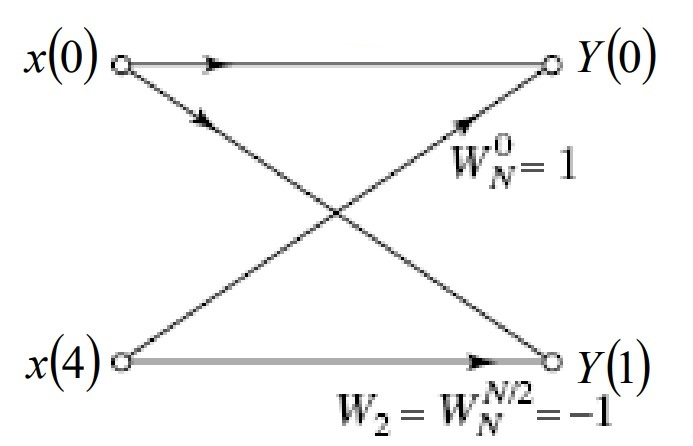
\includegraphics[width=4cm]{fft-dec-graph-bin}
			\caption{graph representation of the \fft using the decimation in time algorithm computed on 2 points starting from a signal of length $N=8$.} \label{fig:dft:fftsing}
		\end{SCfigure}
		
		Reached this point, as shown in figure \ref{fig:dft:fftsing}, we can see that we have only two twiddle factors (that in this case are all real-evaluated) $W_N^0 = 1$ and $W_2 = W_N^{N/2} - 1$ that allows to compute the 2 spectral component of the bisected signal as
		\[ X(0) = x(0) + x(1) \hspace{2cm} X(1) = x(0)- x(1) \]
		
		\begin{figure}[b!t]
			\centering
			\begin{subfigure}{0.48\linewidth}
				\centering 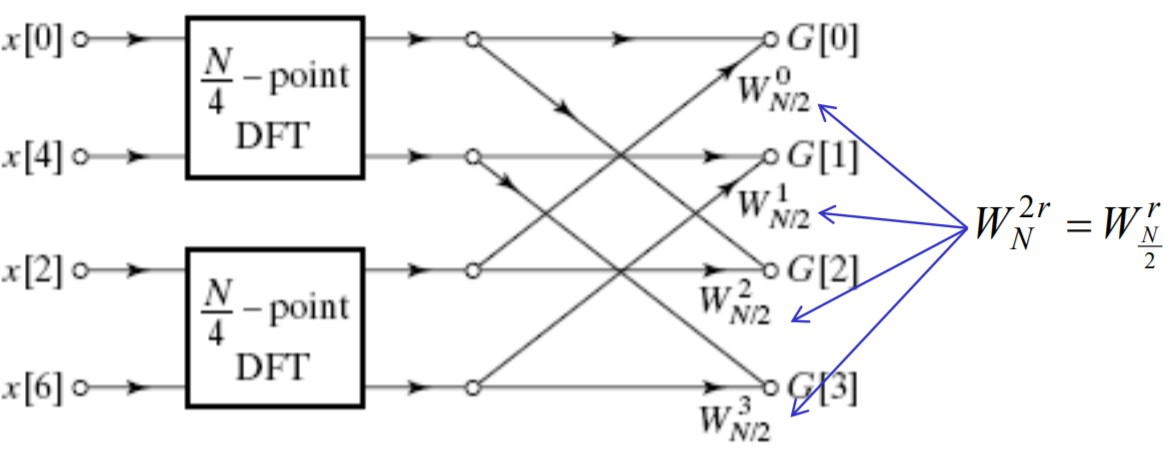
\includegraphics[width=0.9\linewidth]{fft-dec-graph-sec} \caption{}
			\end{subfigure}
			\begin{subfigure}{0.48\linewidth}
				\centering 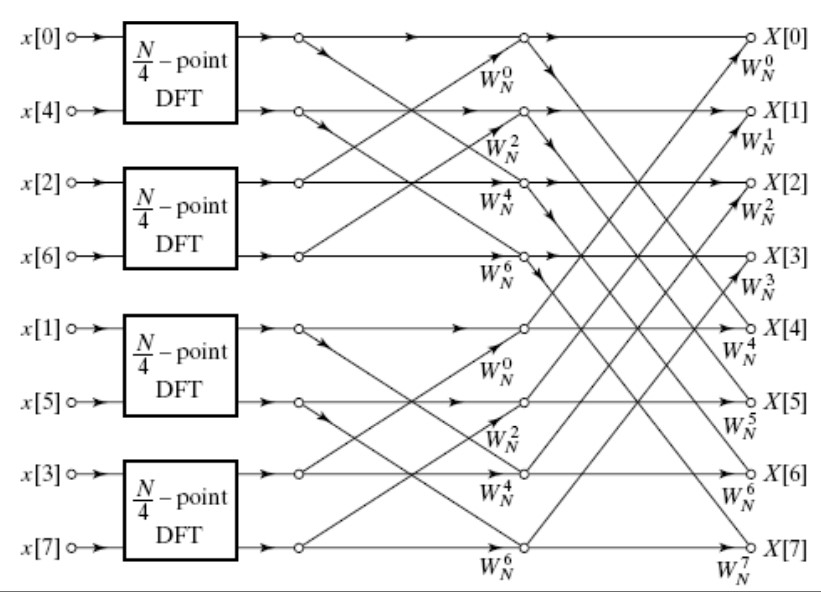
\includegraphics[width=\linewidth]{fft-dec-graph-comp} \caption{}
			\end{subfigure}
			\caption{second (a) and third (last) (b) step of the computation of the DFT on a signal having $N=8$ samples using the decimation in time FFT algorithm.} \label{fig:dft:fftcomp}
		\end{figure}
		
		With the smallest spectra computed, the spectrum re-combination can take place as shown in figure \ref{fig:dft:fftcomp}; considering the second stage of the decimation in time algorithm (fig. \ref{fig:dft:fftcomp}.a) the 4 spectral components are computed as linear combination of 2 elements retrieved one each from the 2 sub-computed spectra of the first stage. The twiddle factors are computed considering the properties $W_N^{2r} = W^r_{N/2}$. The third stage spectral components are so a linear combination of 2 elements from the previous  recursive definition and the recursion keeps going on until reaching the full spectrum of the signal.	 	
		
		\paragraph{Modularity of the decimation in time algorithm} A point of force of the decimation in time FFT algorithm is it's recursion and modularity mainly determined by the \textit{butterfly structure} (name took by the butterfly-look-like graph in figure \ref{fig:dft:fftsing}) and in particular we can observe that
		\begin{itemize}
			\item the algorithm cleverly uses the memory: results of the iterative-recursive stages can be overwritten in the same memory address. The out-of-order samples (as seen on the left side in figure \ref{fig:dft:fftcomp}.b) can be in fact accessed using reversed-bit mode available in all digital signal processing processors:
			\begin{center}
			\begin{tabular}{ M{1cm} M{1.3cm} M{1.3cm} M{1cm} }
				& index & address & \\ \hline
				$x(0)$ & 000 & 000 & $X(0)$ \\ 
				$x(4)$ & 100 & 001 & $X(1)$ \\
				$x(2)$ & 010 & 010 & $X(2)$ \\
				$x(6)$ & 110 & 011 & $X(3)$ \\
				$x(1)$ & 001 & 100 & $X(4)$ \\
				$x(5)$ & 101 & 101 & $X(5)$ \\
				$x(3)$ & 011 & 110 & $X(6)$ \\
				$x(7)$ & 111 & 111 & $X(7)$
			\end{tabular}
			\end{center}
			
			\item the butterfly computation can extended not just to the first stage, but for any $m$-th stage. Considering in fact the spectral components coming from the $X_{m-1}(p),X_{m-1}(q)$ the $m-1$-th stage, the new computed spectral components of the $m$-th stage are stored in the same spot and it happens that
			\begin{equation}
				X_m(p) = X_{m-1}(p) + W_N^r X_{m-1}(q) \hspace{0.5cm} X_m(p) = X_{m-1}(p) - W_N^r X_{m-1}(q)
			\end{equation}
			where the change of sign on the twiddle factor is obtained considering that
			\[ W_N^{r+ \frac N2} = W_N^r W_N^{N/2} = - W_N^r \]
			where $t$ is the coefficient depending on the stage of calculation.
		\end{itemize}
	
	\subsection{Decimation in frequency}
		
		From every FFT algorithm a dual one can be generated in order to compute the inverse \fft; the \de{decimation in frequency} is in fact the dual \textit{representation} of the decimation in time algorithm that allows to reconstruct a signal in the time domain if it's discrete Fourier transform has a number of sample $N$ that's a power of 2 (so in the form $N=2^\nu$).
		
		\begin{figure}[b!]
			\centering 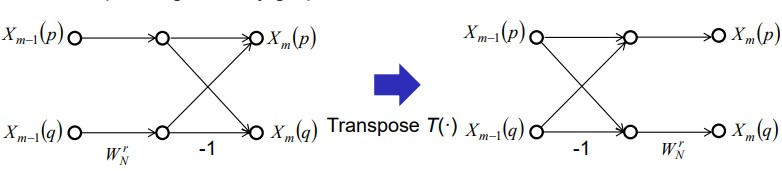
\includegraphics[width=10cm]{fft-dec-stage}
			\caption{graph representation (right) of the decimation in frequency algorithm butterfly as the transposition of the decimation in time one (left).} \label{fig:dft:decfreq}
		\end{figure}
	
		The working principle is the same: the spectrum $X(k)$ is recursively bisected in it's even $X_e(k) = X(2k)$ and odd $X_o(k) = X(2k+1)$ \textit{part} until reaching the recursion limit of a sequence of length $2$. From this point on the butterfly graph to implement, as shown in figure \ref{fig:dft:decfreq} is the transposed one of the decimation in time.
		
		\paragraph{Graph transposition} Given a graph $\delta(N,\varepsilon)$ of $N$ edges $\varepsilon$, then it's transition $\delta^t(N,\varepsilon')$ is obtained by reversing the direction of the edges: the input so becomes the output and vice-versa. The weight of the edges stays unaltered.		
			
\section{Spectral estimation}
	
	The \de{spectral  estimation} is the analysis of signals using techniques in the frequency domain in order to provide informations regarding the behaviour of the system. Real signals are usually stochastic (and not deterministic) and so computing the proper spectra isn't in general a easy problem. Depending on the type of process we are analysing we can classify the signals and so the techniques that can be used as shown in table \ref{tab:dtf:specestim}
	
	
	\begin{table}[bht]
	\centering
	\tabrule
	\caption{spectral estimation classifications.} \label{tab:dtf:specestim} \vspace{2mm}
	
	\begin{tabular}{ M{0.22\linewidth} M{0.22\linewidth} | M{0.22\linewidth} M{0.22\linewidth} }
		\multicolumn{4}{c}{\textbf{Spectral Estimation}} \\  \\ 
		\multicolumn{2}{c|}{deterministic signals (finite energy)} & \multicolumn{2}{c}{random processes (finite power)} \\ &&&\\
		stationary & non-stationary & stationary & non-stationary \\
		$\Downarrow$ & $\Downarrow$ & $\Downarrow$ & $\Downarrow$ \\
		Fourier transform & short-time Fourier transform & power spectral density (PSD) & PSD as a function of time \\
		$\Downarrow$ & $\Downarrow$ & $\Downarrow$ & $\Downarrow$ \\
		DTF/FFT & Discrete STFT & average periodogram and other estimators & spectrogram, short-time periodogram		
	\end{tabular}\vspace{3mm}	
	\tabrule
	\end{table}
	
	If a system is stationary the quality of the estimation doesn't depend on the time on which we perform the estimation itself, while this isn't true for non-stationary signals on we we want to track all the changes of the signal over time.
	
	\subsection{Stationary deterministic signal}
		
		Focusing on the case of a continuous-time \textbf{stationary deterministic signal} $x_c(t)$, the ideal way to perform a spectral estimation is by \textit{simply} computing its \ctft in order to determine the spectrum $X_c(\Omega)$. This is easier said than done, and in real application such operation is not feasible and to do so we necessarily need to discretize the time axis with a certain sampling period $T_s$  and estimate a discrete spectrum $\hat X_c(\Omega) \approx X_c(\Omega)$.
	
		\begin{figure}[bht]
			\centering
			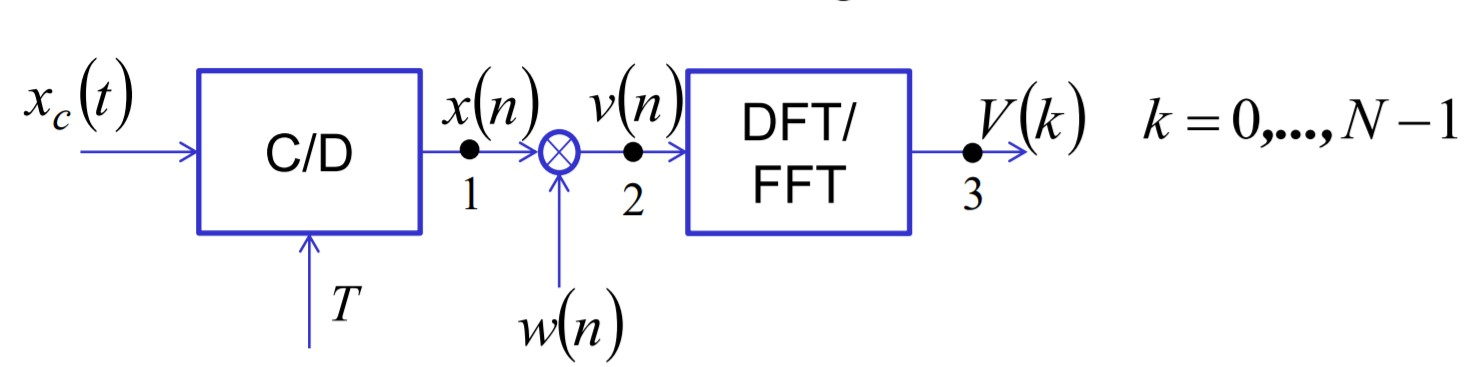
\includegraphics[width=8cm]{deterministic-estimation}
			\caption{steps that has to be performed in order to estimate a stationary deterministic signal.}
			\label{fig:dft:statdetsignalestimation}
		\end{figure}
		
		As it can be seen in figure \ref{fig:dft:statdetsignalestimation}, to perform the estimation we firstly discretize the signal into a discrete-time sequence $x(n)$, determining a change of the original spectrum $X_c(\Omega)$ with the addition of aliases in the transform (as it was discussed in section \ref{sec:conv:timeconversion}, page \pageref{sec:conv:timeconversion}):
		\begin{equation}
			X\big(e^{j\omega}\big) = \frac 1 {T_s} \infsum k X_c\left( \frac \omega{T_s} + \frac{2\pi k}{T_s} \right)
		\end{equation}
		
		After that we have to consider that not physically/computationally feasible to determine the \dtft of a signal with infinite length (it's impossible to store such quantity of data and compute the DFT on it), and so we have to rely on just a \textit{segment} of the whole data. Considering a rectangular \textbf{window} of $L$ samples defined as
		\[ w(n) = \begin{cases}
			1 \qquad & n = 0,\dots, L-1 \\ 0 &\textrm{otherwise}
		\end{cases} \]
		then the signal $v(n)$ that can be processed is the one obtained by multiplying such window with the discretized sequence $x(n)$:
		\[ v(n) = x(n)w(n) \]
		This means that the spectrum that we can estimate is also influenced by the convolution  of the two signals considering the related property and so
		\begin{equation}
			V\big(e^{j\omega}\big) = X\big(e^{j\omega}\big) * W\big(e^{j\omega}\big) = \frac 1{2\pi} \int_{-\pi}^\pi X\big(e^{j\theta}\big) W\big(e^{k(\omega-\theta)}\big)\, d\theta \neq X\big(e^{j\omega}\big)
		\end{equation}
		\begin{note}
			in general other windowing function $w(n)$ can be used (as it's going to be explained later) in order to differently affect the spectral estimation.
		\end{note}
	
		From a practical point of view the only way to estimate the spectrum is by computing the \dft $V(k)$, a \textit{sampled} version of the \textit{continuous} spectrum $V(e^{j\omega})$ in the frequency domain. As a rule of thumb the discretization value $N$ for the 	DFT computation should always be grater (or equal) to the length $L$ of the window (in order not to have the time aliasing problem while returning in the time domain after signal processing).	
		
		\subsubsection{Effect of windowing on the spectral estimation of a cosine wave} Considering the continuous-time sinusoidal signal $x_c(t) = A \cos(\Omega_0 t +\theta_0)$, as was previously seen, it's spectrum (shown in figure \ref{fig:dft:cosinespectrum}) consists of two dirac pulses at frequencies $\pm \Omega_0$ with a complex amplitude of $\frac A 2 e^{-j\theta_0}$.
		
		\begin{SCfigure}[2][bht]
			\centering 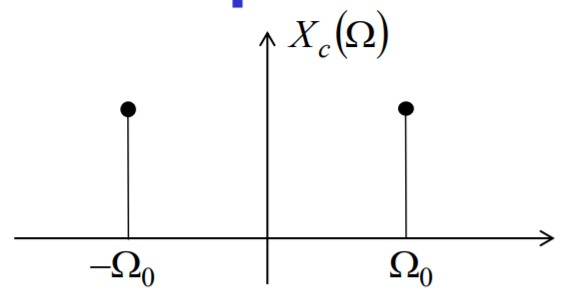
\includegraphics[width=5cm]{sin-spect}
			\caption{magnitude spectrum of the signal $A \cos(\Omega_0t+\theta_0)$.}
			\label{fig:dft:cosinespectrum}
		\end{SCfigure}
		
		Considering it's discretized version $x(n) = A\cos(\omega_0n + \theta_0)$ (where $\omega_0 = \Omega_0 T_s$) then the windows signal $v(n)$ on which the DFT can be computed is
		\begin{align*}
			v(n) & = x(n) w(n) = A w(n)\, \cos(\omega_0n + \theta_0) \\
			& = \frac A 2 w(n) e^{j\theta_0} e^{j\omega_0n} + \frac A 2 w(n) e^{-j\theta_0} e^{-j\omega_0n} 
		\end{align*}
		Knowing the \dtft of the signal $e^{j\omega_0n}$ as $\delta(\omega-\omega_0)$, then the spectrum $V(e^{j\omega})$ of the sequence can be regarded
		\begin{equation} \label{eq:dft:windowedcosine}
			V \big(e^{j\omega}\big) = \frac A 2 e^{j\theta_0} W\big( e^{j(\omega-\omega_0)}\big) +  \frac A 2 e^{-j\theta_0} W\big( e^{j(-\omega+ \omega_0)}\big)
		\end{equation}
		
		To determine the \textit{distortion} due to the window it's necessary to compute it's spectrum; considering in fact the sequence $w(n) e^{-j\omega n}$ the DTFT is computed as
		\begin{align*}
			W\big(e^{j\omega}\big) & = \infsum n w(n) e^{-j\omega n} = \sum_{n=0}^{L-1} e^{-j\omega n} = \frac{1-e^{-j\omega L}}{1-e^{-j\omega}} \\
			& = e^{-j\omega \frac{L-1}{2}} \frac{\sin\left(\frac{\omega L}{2}\right)}{\sin\left(\frac \omega 2\right)}
		\end{align*}
		\begin{note}
			the \dtft  of the window has been computed the convergent geometrical sequence summation described in the note at page \pageref{sec:four:geometricalprogression}.
		\end{note}
		The term $\frac{\sin(\omega L/2)}{\sin(\omega/2)}$ is known as the \de{Dirichlet-Kernel} function characterized by being equal to $L$ for $\omega_0$ and being null for each multiple of the frequency $\frac{2\pi}{L}$; in figure \ref{fig:dft:dirichkernel} it's spectrum has been represented.
		
		\begin{figure}[bht]
			\begin{subfigure}{0.48\linewidth}
				\centering 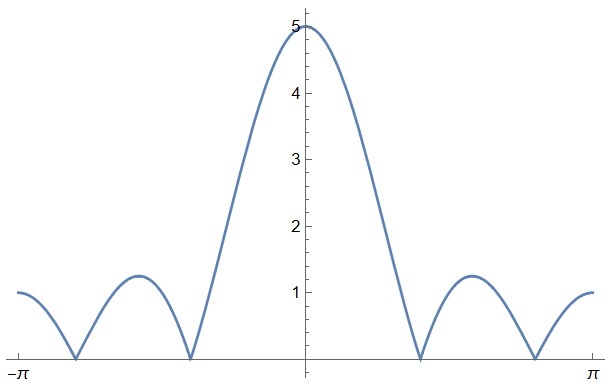
\includegraphics[width=5cm]{dirich-kernel} \caption{}
			\end{subfigure}
			\begin{subfigure}{0.48\linewidth}
				\centering 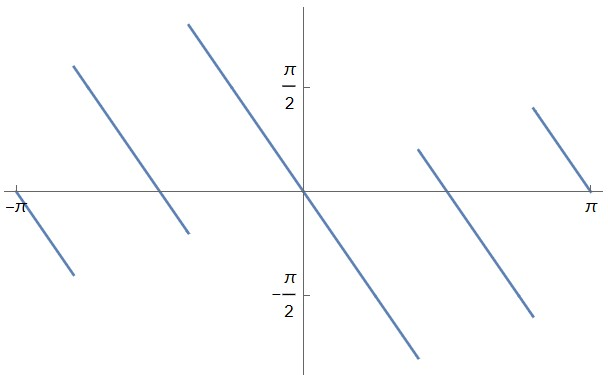
\includegraphics[width=5cm]{dirich-kernel-phase} \caption{}
			\end{subfigure}
			\caption{magnitude (a) and phase (b) of the Dirichlet-Kernel function.}
			\label{fig:dft:dirichkernel}
		\end{figure}
		
		\noindent For this Dirichlet-Kernel function we refer the \textit{central peek} as the \textbf{main-lobe} (with a peak equals to $L$) while the other \textit{bell-shaped} segments are referred as \textbf{side-lobes}; this function is characterized by the main-lobe width $\Delta_w = 4\pi/L$ parameter; we can also observed that the spectrum (figure \ref{fig:dft:dirichkernel}.b) has a so called \textbf{\textit{generalized linear phase}}. \vspace{3mm}
		
		With the definition of the Dirichlet-Kernel function, the spectrum of the windowed cosine function (equation \ref{eq:dft:windowedcosine}) isn't just made of two pulses at frequencies $\pm \omega_0$, but it's composed by two Dirichlet-Kernel functions with main-lobes center at frequencies $\pm\omega_0$ (on which the pulses were expected), as shown in figure \ref{fig:dft:spectrdistorted}.
		
		\begin{SCfigure}[2][bht]
			\centering 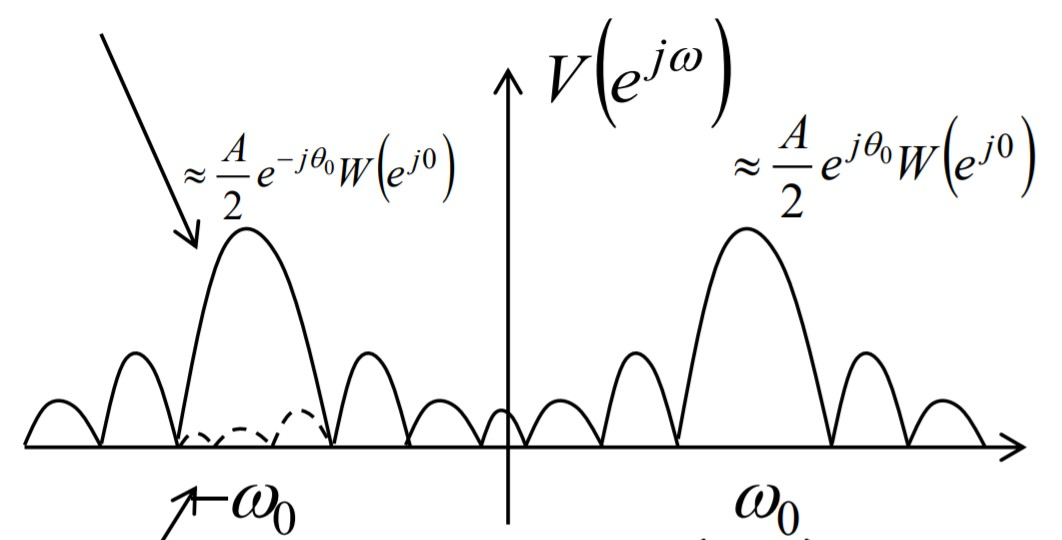
\includegraphics[width=6cm]{sin-modified}
			\caption{spectrum of the signal  $v(n)= x(n)w(n)$ that's distorted due to the windowing.}
			\label{fig:dft:spectrdistorted}
		\end{SCfigure}  
	
		To reduce the effect ot the lobes of the Dirichlet-Kernel function it's necessary to reduce the main-lobe width $\Delta_w$ by increasing the number of samples $L$ collected by the window (for $L\rightarrow \infty$ the Dirichlet-Kernel tends to the Kronecker delta). Practically this operation of increasing the length of samples $L$ can be pushed up to a certain limit (time/numerical complexity) and the problem that we get from this limitation are
		\begin{itemize}
			\item the \textbf{spectral leakage}: considering the case shown, the theoretical energy of the sinusoidal signal is concentrated at the frequencies $\pm\omega_0$, however with the addition of the windowing there's a sort of \textit{leak} that spreads out the energy all over the frequency axis;
			
			\item the \textbf{spectral infiltration}, related to the leakage, refers to the fact that the principal side-lobes (the ones next to the main-lobe) might interfere with main-lobes of other function's transforms. It can be noted that the ratio between main and principal side-lobe is constant and weakly depends on the number of samples $L$;
			
			\item the \textbf{finite spectral resolution}: considering a signal that's a sum of cosine function of the form $x_c(t) = A_1 \sin(\Omega_1t + \theta_1) + A_2 \sin(\Omega_2t+\theta_2)$, then the theoretical DTFT consists of dirac pulses centred at the frequencies $\pm \omega_1,\pm \omega_2$, however the estimated spectrum due to the window is
			\[ V \big(e^{j\omega}\big) = \sum_i \frac{A_i}{2} e^{\pm j\theta_i} W\Big( e^{j(\omega \mp \omega_i)} \Big) \]
			Depending on the length $L$ of the window, if the frequencies $\omega_1,\omega_2$ are \textit{sufficiently close together} the main-lobes associated related to the windows of the cosine might interfere (as shown in figure \ref{fig:dft:spectralresolution}). In order to avoid such problem we have to ensure that
			\[ |\omega_1-\omega_2| > \frac{\Delta_w}{2} \]
			
		\end{itemize}
	
		\begin{SCfigure}[2][bht]
			\centering 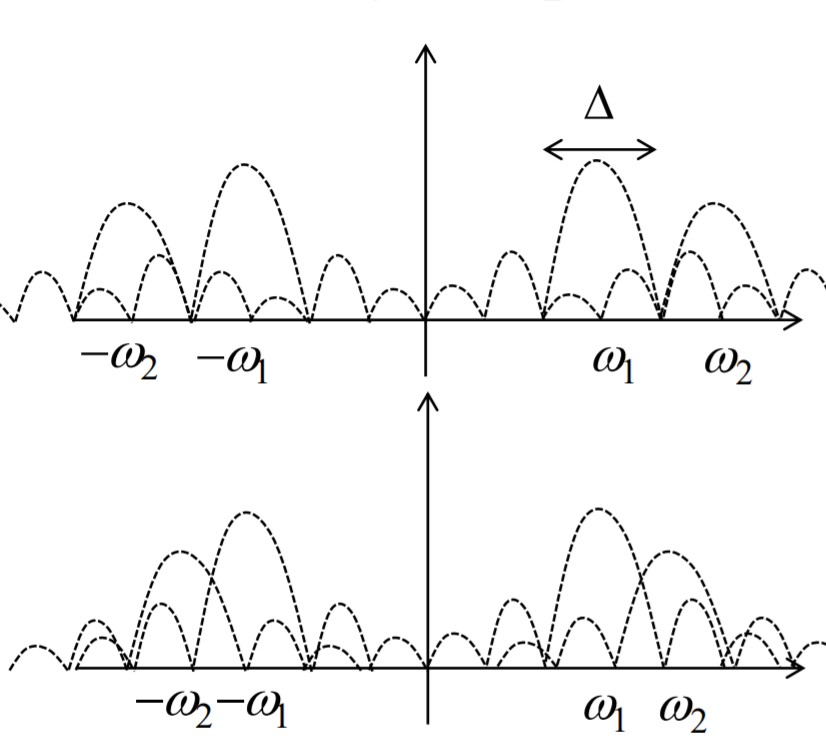
\includegraphics[width=6cm]{spectral-resolution}
			\caption{estimated spectrum of a signal $ A_1 \sin(\Omega_1t + \theta_1) + A_2 \sin(\Omega_2t + \theta_2)$ where the difference $\omega_1-\omega_2$ is "big" and so the spectral leakage can be neglected (upper) and the case on which the frequencies are "sufficiently close" (lower) considering the problem of the spectral resolution.} \label{fig:dft:spectralresolution}
		\end{SCfigure}
	
		\subsubsection{Windowing functions}
		In general other windowing function $w(n)$ different from the rectangular one can be constructed in order to minimize the errors/problem related to the spectral estimation. Performances can be improved by increasing, as example, the ratio between the main-lobe and the principal side-lobes or lowering the main-lobe width $\Delta_w$ for the same window length $L$. In figure \ref{fig:dft:windowfunctions} a set of windowing functions have been presented in both the time domain and frequency magnitude response.
		
		\begin{figure}[bht]
			\centering 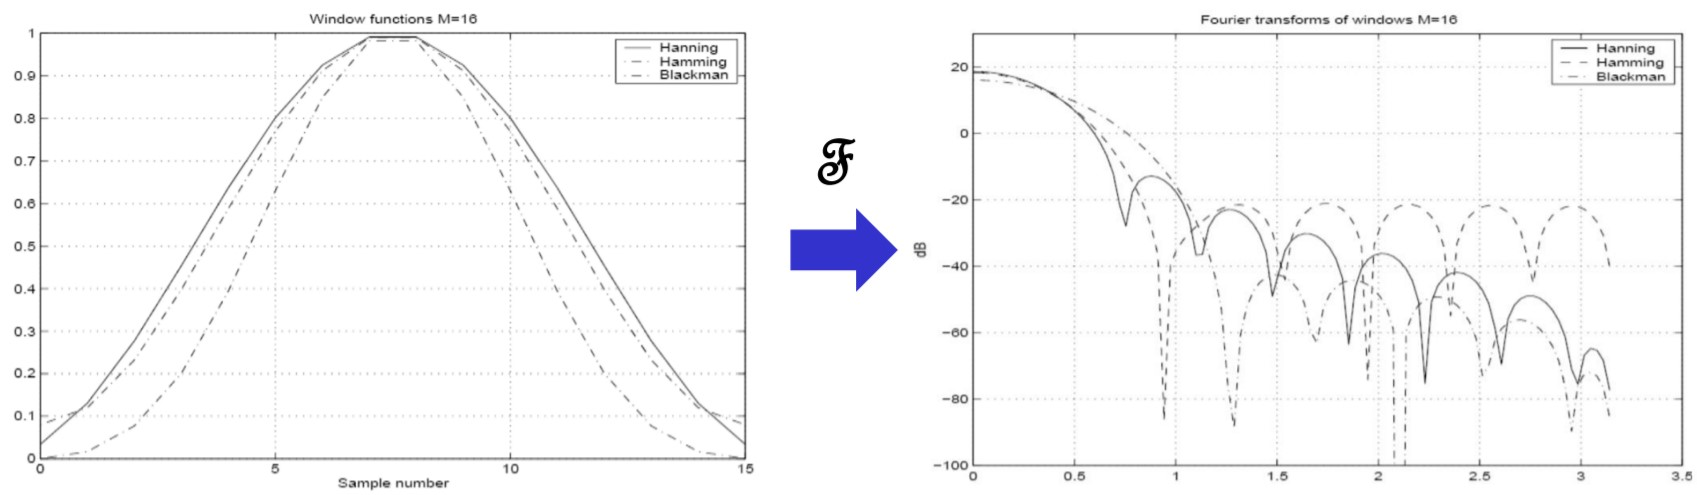
\includegraphics[width=\linewidth]{windowfunctions}
			\caption{windowing functions and relative magnitude of the Fourier transforms.}
			\label{fig:dft:windowfunctions}
		\end{figure}
		
		Table \ref{tab:dft:windowfunctions} resumes the main characteristics of some window functions; in particular we can see that (for a fixed length $L$ of the window) the side/main-lobe ratio is inversely proportional to the main-lobe width (lower $\Delta_w$ positively affects the resolution with the drawback of a higher \textit{side-lobe infiltration} impact).
		
		\begin{table}[bt] \centering \tabrule
			\caption{list of possible windows with relative side to main-lobe radio (in decibels) and main-lobe width (depending on number of windowed samples $L$); the maximum ripple amplitude error $\varepsilon$ is also presented due to it's relevance in the digital filter design described on chapter \ref{sec:digitalfilterdesign}.}
			\label{tab:dft:windowfunctions}
			\begin{tabular}{M{0.2\linewidth} M {0.2\linewidth} M{0.2\linewidth} M{0.2\linewidth} }
				window & side/main-lobe ratio & main-lobe width $\Delta_w$ & $\varepsilon$\\ \hline
				rectangular & $-13db$ & $4\pi/L$ & $-21dB$ \\
				Bartlett (triangular) & $-25db$ & $8\pi/L$ & $-25dB$ \\
				Hanning & $-31db$ & $8\pi/L$ & $-44dB$ \\
				Hamming & $-41db$ & $8\pi/L$ & $-53dB$ \\
				Blackman & $-57db$ & $12\pi/L$ & $-74dB$ \\
			\end{tabular} \vspace{2mm}\tabrule
		\end{table}
	
		\paragraph{Cosine class windows} The \textbf{Hanning}, \textbf{Hamming} and \textbf{Blackman} functions belongs to the \de{cosine class windows} of order $K$ whose general formulation is
		\begin{equation} \label{eq:dft:cosinewindows}
			w(n) = \sum_{k=0}^K a_k \cos \left(\frac{2\pi k}{L}n\right)\, dk
		\end{equation}
		Hanning and Hamming are both first order cosine windows with respective coefficients $a_0 = \frac 1 2,a_1 = - \frac 1 2$ and $a_0 = 0.54,a_1 = -0.46$; the Blackman filter is instead a second order filter. The general formulation of the main-lobe width of cosine-class function is
		\begin{equation}
			\Delta_w = \frac{4\pi}{L} \big(K+1\big)
		\end{equation}
		
		Respect to table \ref{tab:dft:windowfunctions}, fixed the length $L$ of the window going from the rectangular to the Blackman window worsen the resolution while improving on the spectral leakage side (and so is always a tradeoff between this two characteristic: resolution vs spectral leakage).
		
		\subsubsection{Frequency discretization}
		Until now we referred to the \dtft $V\big(e^{j\omega}\big)$ of the sampled signals, however in practise the tool that we can use is the \dft (FFT algorithms) computing the discretized spectrum $V(k)$. Considering, as reference, the case of the co-sinusoidal function whose transform is described in equation \ref{eq:dft:windowedcosine}, the choice of the number $N$ of frequency discretization heavily affects the read of the spectrum itself; for that reason 3 particular scenarios (graphed in figure \ref{fig:dft:samplingvariation}) can happen:
		\begin{enumerate}
			\item \textbf{coherent sampling} happens when one of the spectral sample lies exactly at the frequency $\omega_0$ while the other samples coincides with the zeros of the window spectrum; in this case the spectrum is clearly read by the DFT and the effect of leakage is negligible. This kind of operation can be performed in general only for periodic signals (on which it's relatively \textit{easy} to determine the number of samples $N$ that minimises the leakage) due to the fact that the ideal spectrum is composed by a sequence of pulses;
			
			\item \textbf{non-coherent sampling} happens when the peak lies between the two spectral samples; in this case there's \textit{a lot} of uncertainty in both magnitude and phase response of the expected frequency peak due to the evident effect of spectral leakage;
			
			\item increasing the number of samples in a non-coherent sampling improves estimation by having a higher frequency resolution (that doesn't mean having a higher quality estimation) but that doesn't get rid of the spectral leakage that's still present.			 
		\end{enumerate}
		
		\begin{figure}[bt]
			\begin{subfigure}{0.32\linewidth}
				\centering 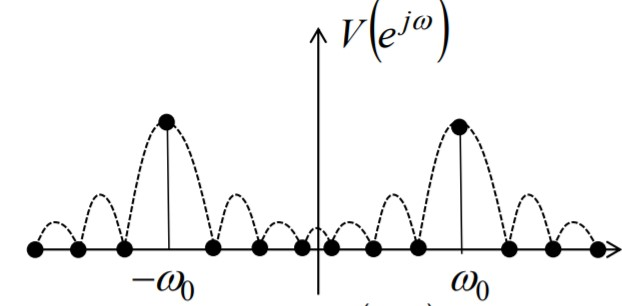
\includegraphics[width=0.9\linewidth]{sampling-1} \caption{}
			\end{subfigure}
			\begin{subfigure}{0.32\linewidth}
				\centering 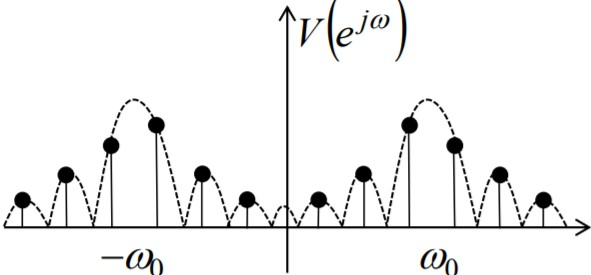
\includegraphics[width=0.9\linewidth]{sampling-2} \caption{}
			\end{subfigure}
			\begin{subfigure}{0.32\linewidth}
				\centering 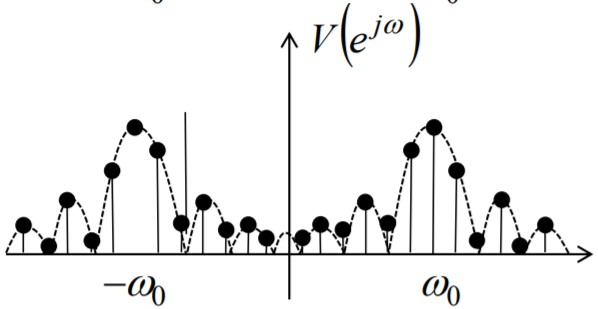
\includegraphics[width=0.9\linewidth]{sampling-3} \caption{}
			\end{subfigure}
			\caption{coherent sampling (a), non-coherent sampling (b) and non-coherent sampling with higher number of samples $N$ (c).}
			\label{fig:dft:samplingvariation}
		\end{figure}
				
	\subsection{Non-stationary deterministic signal: short time Fourier transform}
		
		A simple example of \textbf{non-stationary deterministic signal} is a sinusoidal function with frequency changing over time:
		\[ x_c(t) = \cos\big(\Omega(t)\,t\big)  \hspace{2cm} \text{where } \Omega(t) = \Omega_0 t \]
		Evaluating this signal at a time $t_0$ we expect, as spectral response, a Dirac pulse centred at the frequency $\pm \Omega(t_0)$, but if we evaluate the same signal at another time $t_1\neq 0$ such pulses are shifted to different frequencies $\Omega(t_1)$.
		
		In practise the tools that we can use to perform the spectral estimation is the \dft applied on a finite window of length $L$ of the samples signal $x(n)$. Reading so the spectrum of the signal in example will result in a \textit{smoothed average} of the peaks in the transform in the range whose samples are extracted.\\
		To reduce the \textit{average effect} we can try to reduce the window in the time domain by lowering the interval $\Delta t$, however this negatively effects the number of recorded samples $L$ (that decreases the frequency resolution having less frequency discretization), and so as a rule of thumb we have to consider that:
		\begin{align*}
			\text{long window} \qquad & \Rightarrow \qquad \text{high frequency resolution, poor time resolution} \\
			\text{short window} \qquad & \Rightarrow \qquad \text{low frequency resolution, high time resolution} \\
		\end{align*}
	
		Considering a time window $\Delta t = t_2-t_1$, the expected frequency peaks at the start of the estimation is $\Omega_1$ and at the end is $\Omega_2$ and so the normalized frequency (depending on the sampling period $T_s$) is
		\[  \Delta \omega = \Delta \Omega\, T_s \]
		Considering that such difference should be greater than half of the main-lobe width, considering a rectangular window we retrieve the following expression relating the time difference (associated to the time resolution) and the variation of the analysed frequency components (frequency resolution):
		\begin{equation}
			\Delta \omega = 2 \pi \, \Delta f > \frac{\Delta_w}{2} == \frac{4\pi}{2L} \hspace{1.2cm} \Rightarrow \hspace{1.2cm} \Delta f \, LT_s = \Delta f\, \Delta t > 1
		\end{equation}
		
		\subsubsection{Short-time Fourier transform}
		The \de{short-time Fourier transform}, also referred as \textbf{discrete-time time-varying Fourier transform}, is a particular transform used to estimate the spectral behaviour of non-stationary deterministic signals.
		
		The main idea of such operation is to perform DFTs over a window of $L$ samples that shifts each time by $R$ samples. Considering the DTFT definition of a sequence $x(n)$ as
		\[ X\big(e^{j\omega}, n\big) = \sum_{m=0}^{L-1} x(n+m)\, w(m) e^{-j\omega m} \]
		Applying the DFT on such spectrum and shifting by a multiple $r$ of $R$ samples we obtain:
		\begin{equation}
			X_r(k) = \sum_{m=0}^{L-1} x\big(rR+m\big) w(m) e^{-j\frac{2\pi}{N}mk}
		\end{equation}
		In practise relation between the sample shift $R$, the window length $L$ and the frequency discretization $N$ used by the DFT is
		\[ R \leq L \leq N \]
		The first inequality ensures that no samples are skipped (resulting in a loss of information), while the second ensure a better read-out of the spectrum.
		
		The short-time Fourier transform present a better \textit{tracking capability} of time changes respect to the common of the DFT with the computational drawback higher processing power (resulting in difficulties if the signals must be elaborated in real time).
		
	\subsection{Stationary random processes: power spectral density estimation}
		As was discussed in section \ref{sec:prob:psd} (page \pageref{sec:prob:psd}), the \textbf{power spectral density} $\Phi_X(e^{j\omega})$ was described as the \textbf{autocorrelation} of \textbf{wide-sense stationary} random processes (eq. \ref{eq:prob:psd}). For real world application, estimating such spectrum is way much heavier than a single DFT due to the fact that the autocorrelation contains a summation in it's definition.
		
		Given so a continuous signal $x_c(t)$ (realization of a wide-sense stationary random process) sampled with a period $T_s$ determining the sequence $x(n)$ windowed by the signal $w(n)$, the estimation of the power spectral estimation can be achieved mainly in two ways:
		\begin{enumerate}
			\item computing firstly the auto-correlated windowed signal using the formal definition of correlation (equation \ref{eq:four:correlation}, page \pageref{eq:four:correlation}); in particular considering the rectangular window of $L$ samples the autocorrelation of the signal $v(n) = x(n) w(n)$ can be regarded as
			\begin{equation} \label{eq:dft:windowedautocorr}
				\hat \phi_v(n) = \frac 1 L \sum_{l=0}^{L-|n|-1} x(l) x(n+1) \hspace{2cm} \textrm{with } n = 0,\dots, L-1 
			\end{equation}
			To complete the spectral estimation of the power spectral density $\Phi_v\big(e^{j\omega}\big)$ we can compute the Fourier transform on the computed autocorrelation signal $\hat \Phi_v\big(e^{j\omega}\big) = \four{\hat \phi_v(n)}$.
			
			\item by \textit{reversing} the steps the idea is to firstly determine the DFT spectrum $V(k)$ of the windowed signal $v(n)$ and then using a \textit{power spectral density \textbf{estimator}} that compute the estimate $\hat \Phi_v\big(e^{j\omega}\big)$ (or in practise it's discretization) directly in the frequency domain; this operation is performed by the so called \de{periodogram} (that will be described later).			 
		\end{enumerate}
	
		\subsubsection{Estimator}
		An \de{estimator} is any function that, given a random sample from a population, infers a parameter of the population that the samples is taken from.\\
		An example of estimator $E\{\cdot\}$ is the operator that, given $M$ person randomly extracted by the inhabitants of a city, infers the average age of the city; in this simple case the estimator is simply the mean value
		\[ E\{x\} = \frac 1 M \sum_{i=1}^M x_i \]
		
		\paragraph{Power spectral density estimator} The goal now is to define a function $g$ that better estimates the power spectral density of a given transformed sequence (that's so in the frequency domain). Considering $\underline x$ as the random vector of all the possible inputs of the function, then the estimated power spectral density $\hat \theta  = g(\underline x)$ becomes a random process  with stochastic input $\underline x$ and $\theta$ as it's realization.
		
		Considering $\hat \theta$ as a random process, then it's characterized by a probability density function that allows to compute the expected value $E\{\hat \theta\}$ and it's variance $\var{\hat \theta}$ that, in the ideal case, must be
		\[ E\{\hat \theta\} = \theta \hspace{3cm} \var{\hat \theta} = 0 \]
		Such conditions aren't always satisfied and so we can defined the estimator $g$ based on it's performance with the following orthogonal criteria:
		\begin{equation}
		\begin{aligned}
			E \{\hat \theta\} = & \begin{cases}
				\theta \qquad & \text{: unbiased estimator} \\
				\theta + c \qquad & \text{: biased estimator} 
			\end{cases}\\
			\var{\hat \theta} \xrightarrow{M\rightarrow 0} & \begin{cases}
				= 0  & \hspace{6pt} \text{: consistent estimator} \\
				\neq 0  &\hspace{6pt} \text{: inconsistent estimator} 
			\end{cases}
		\end{aligned}
		\end{equation}
		
		In general problems regarding the bias of the estimator can be somehow handles while the same cannot be said for the consistency regarding the variance: for this reason is preferable a consistent but biased estimator then a biased-inconsistent one.
		
		\paragraph{Characteristic of the estimation from the computation of the autocorrelation} Given the windowed signal $v(n) = x(n)w(n)$, equation \ref{eq:dft:windowedautocorr} described it's autocorrelation (in the case of rectangular window); computing on such definition the expectation operator we observe that
		\begin{equation}
		\begin{aligned}
			E\left\{ \hat \Phi_V(n) \right\} & = E \left\{ \frac 1 L \sum_{l=0}^{L-|n|-1} x(l) x(n+1) \right\} = \frac 1 L \sum_{l=0}^{L-|n|-1} \phi_x(n) \\ 
			& = \frac{L-|n|}{L} \phi_x(n)
		\end{aligned}
		\end{equation}
		From this definition we can describe this estimation as biased with a non-constant bias level depending from the length $L$ of the window and the \textit{position} $n$ of the sample that we consider for the estimation; in general the non-linearity effect can be neglected if $n \ll L$. Similarly it can be proven that this estimator is inconsistent, in fact
		\begin{equation}
			\var{\hat \Phi_V(e^{j\omega})} = E \left\{ \hat \Phi_v^2(n) \right\} - E^2 \left\{ \hat \Phi_v (n) \right\} = \alpha \phi_x^2 (n)
		\end{equation}
		
		\subsubsection{Periodogram}
		The \de{periodogram} is a particular \textbf{power spectral density estimator} defined for both DTFT and DFT as
		\begin{equation} \label{eq:dft:periodogram}
			\hat \Phi_V(\cdot) = \frac{|V(\cdot)|^2}{L}
		\end{equation}
		where $V(\cdot)$ is the Fourier transform of the windowed signal $v(n)$. By extending both the definition of the \dtft we can reconsider the estimator as
		\begin{align*}
			\hat \Phi_V(e^{j\omega}) & = \frac 1 L \Big( \sum_{n=-\infty}^\infty x(n) w(n) e^{-j\omega n} \Big)\Big( \sum_{m=-\infty}^\infty x(n) w(n) e^{-j\omega m} \Big)^* \\ & = \frac 1 L \Big( \sum_{n=-\infty}^\infty x(n) w(n) e^{-j\omega n} \Big) \Big( \sum_{m=-\infty}^\infty x^*(n) w(n) e^{j\omega m} \Big) \\ 
			& = \frac 1 L \sum_{n=-\infty}^\infty\sum_{m=-\infty}^\infty x(n) x^*(m) w(n) w(m) e^{-j\omega(n-m)}
		\end{align*}
		Computing the expectation operator on the periodogram we obtain
		\begin{align*}
			E\left\{ \hat \Phi_V \right\} & = \frac 1 L \sum_{n=-\infty}^\infty\sum_{m=-\infty}^\infty \overbrace{E\left\{x(n) x^*(m)\right\}}^{= \phi_x(m) \textrm{: autocorrelation}} w(n) w(m) e^{-j\omega(n-m)} \\
			\xrightarrow{n-m=k} \quad & = \frac 1 L \sum_{m=-\infty}^\infty \sum_{k=-\infty}^\infty \phi_x(k) w(m) w(m+k) e^{-j\omega k} \\
			& = \frac 1 L \underbrace{\sum_{k=-\infty}^\infty \phi_x(k) e^{-j\omega k}}_{i)} \underbrace{\sum_{m=-\infty}^\infty w(m) w(m+k)}_{ii)}
		\end{align*}
		In this equation the term $i)$ represent the power spectral density value that has to be estimated while $ii)$ is the autocorrelation $\mathcal E_w(k)$ of the window function that can be regarded as a \textit{weight} in the evaluation of the expectation. Applying now to this result the Parseval's theorem (equation \ref{eq:four:parserval}, page \pageref{eq:four:parserval}) then the \textbf{expectation} of the \textbf{periodogram} can be computed as
		\begin{equation} \label{eq:dft:asympunbiased}
			E\{ \hat \Phi_V \} = \frac 1 {2\pi L } \int_{-\pi}^{\pi} \phi_x\big( e^{j\theta}\big) \mathcal C_w \big(e^{j(\omega-\theta)}\big) \, d\theta = \frac 1 L \phi_x\big(e^{j\omega}\big) * \left|W\big(e^{j\omega}\big)\right|^2
		\end{equation}
		With this definition we can observe that the periodogram is biased, however with $L\rightarrow 0$ the expected value tends to $\phi_x(e^{j\omega})$ and for that reason we defined the periodogram as \textbf{asymptotically unbiased}. Considering gaussian processes it still happens that, for $L\rightarrow \infty$, the periodogram is a inconsistent estimator, it can be shown in fact that
		\begin{equation} \label{eq:dft:inconsistency}
			\var{\Phi_V (e^{j\omega})} \propto \Phi_x^2(e^{j\omega})
		\end{equation}
		
		\paragraph{Modified periodogram} Equation \ref{eq:dft:periodogram} defining the periodogram is stated considering the case of a rectangular window, however practical application might require the use of different window function; for this reason the definition of the \textbf{modified periodogram} is regarded as the normalization of the magnitude of the spectrum squared over the energy $E_w$ of the window signal and so
		\begin{equation}
			\hat \Phi_V \big(e^{j\omega}\big) = \frac{\left| V\big(e^{j\omega}\big) \right|^2}{\sum_{i=0}^{L-1} w(n) }
		\end{equation}		
		Similarly as for the \textit{basic} periodogram it can be proven that such definition is still asymptotically unbiased (equation \ref{eq:dft:asympunbiased}) and inconsistent (as in equation \ref{eq:dft:inconsistency}).
		

\section{Examples}
	\subsection{Convolution computation}
		A continuous-time LTI system characterized by a \textit{triangular-shaped} impulse response $h$
		\[ h(t) = \begin{cases}
			t & 0\leq t\leq T \\ 0 & \textrm{otherwise}
		\end{cases} \]
		and is subjected to an unitary rectangular input of duration $T$ starting from $t=0$ described by the function
		\[ x(t) = \begin{cases}
			1 & 0\leq t\leq T \\ 0 & \textrm{otherwise}
		\end{cases} \]
		
		\begin{figure}[bt]
			\centering 
			\begin{subfigure}{0.48\linewidth}
				\centering \includegraphics[width=\linewidth]{ex-conv-1} \caption{}
			\end{subfigure}
			\begin{subfigure}{0.48\linewidth}
				\centering \includegraphics[width=\linewidth]{ex-conv-2} \caption{}
			\end{subfigure}
			\caption{plot of the input $x(t)$ (a) and impulse response $h(t)$ (b) of the system; for this representation a value $T=3$ has been considered.} \label{fig:ex:signals}
		\end{figure}
		
		The output response $y(t)$ of such system can be evaluated so as the convolution $x(t)*h(t)$ in the time domain between the input and the impulse response of the system. As presented in figure \ref{fig:ex:convolution}, the convolution whose formulation was stated in page \pageref{eq:four:convolution} as
		\[ x(t) * y(t) = \int_{-\infty}^\infty x(\tau) h(t-\tau)\, d\tau \]
		can be regarded as the integral of the multiplication of two function: one fixed (formally $x$ in the definition) and one moving ($y$) over time. In this case it makes more sense to \textit{move} over time the rectangular input and so the output (considering the commutative property of the convolution) is computed as
		\[ y(t) = h(t) * x(t) = \intinf h(t\tau)x(t-\tau)\, d\tau \]
		
		\begin{SCfigure}[2][bht]
			\centering \includegraphics[width=0.5\linewidth]{ex-conv-3} 
			\caption{the convolution can be computed considering a fixed signal (in this case $h(t)$ in orange) and a moving one ($x(t)$); the value of the convolution is the integral of the product for each position $\tau$ of the moving function. } \label{fig:ex:convolution}
		\end{SCfigure}
	
		Geometrically to determine such integral we have to consider the \textit{revered} rectangle determined by the expression $x(-\tau)$; until such graphic \textit{is on the left} of the  impulse response function (and so for $t<0$) there's no overlap between the function and so the convolution is identically null; the same can be said when the reversed rectangular signal $x(-\tau)$ is \textit{on the right} (and so for $t>2T$). \\
		For $t$ starting from $0$ and up to $T$ we can see that the rectangle \textit{starts inserting} in the non-zero impulse response region for a quantity $t$, and so by integration we obtain that
		\[ y(t) = \int_0^t \tau\cdot 1\, d\tau = \frac{t^2}{2} \]
		Laterly, for $T\leq \tau \leq 2T$, the rectangle \textit{exits} from the impulse response determining a change in the integration intervals: 
		\[ y(t) = \int_{T-t}^T \tau\cdot 1\, d\tau = -\frac{t^2}{2} + Tt \]
		The complete solution of the convolution, graphed in figure \ref{fig:ex:convolutionresult}, is so described by the expression
		\[ y(t) = \begin{cases}
			0 & t < 0 \textrm{ and } t > 2T \\
			\frac{t^2}{2} & 0\leq t < T \\
			-\frac{t^2}{2} + Tt & T\leq t \leq 2T
		\end{cases} \]
		
		\begin{SCfigure}[2][bht]
			\centering \includegraphics[width=0.5\linewidth]{ex-conv-4} 
			\caption{output $y(t)$ of the system computed as the convolution $h(t)*x(t)$ between impulse response and input sequence. } \label{fig:ex:convolutionresult}
		\end{SCfigure}
		
		
		
		
		
		
%	\subsection{Autocorrelation}
	
	\subsection{Passive low-pass filter and finite difference approach} \label{sec:ex:lowpass}
		
		\begin{SCfigure}[2][bht]
			\centering 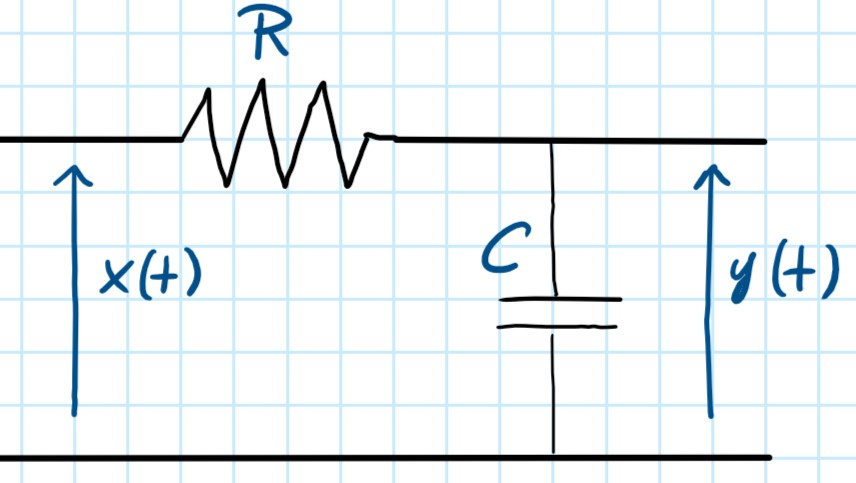
\includegraphics[width=5cm]{passivelowpass}
			\caption{schematic representation of the "common" passive low-pass filter.}
			\label{fig:ex:lowpass}
		\end{SCfigure}
		
		Considering the passive low-pass filer in figure \ref{fig:ex:lowpass} where $x(t)$ is the input voltage and $y(t)$ the output voltage, given $i(t)$ the current passing through the resistor then from the Kirchhoff laws we have to impose the relation
		\[ x(t) = Ri(t) + y(t) \]
		Considering that the current $i(t)$ depends from the voltage difference between the capacitor following the differential equation $i(t) = C\dot y(t)$ then the differential equation solution of the transient is
		\[ x(t) = RC \dot y(t) + y(t) \]
		The solution can be obtained in the frequency domain: applying the \ctft we determine an algebraic equation that can solve the spectrum of the output:
		\[ X(j\Omega) = j\Omega RC Y(j\Omega) + Y(j\Omega) \qquad \Rightarrow \qquad Y(j\Omega) = \frac 1{1 + j\Omega RC} X(j\Omega)\]
		where we can recognize the well-known frequency response $H(j\Omega) = \frac 1{1 + j\Omega RC}$ of the low pass filter that by inversion determines the impulse response
		\[ h(t) = \frac 1{RC} e^{-\frac{t}{RC}} u(t) \hspace{2cm} u(t) = \begin{cases}
			1 & t\geq 0 \\ 0 & t < 0
		\end{cases} \]
		\begin{note}
			when the Fourier transform was applied on the differential equation as initial condition a value $y(0)= 0$ has been set.
		\end{note}
		\begin{SCfigure}[2][bht]
			\centering \includegraphics[width=4.5cm]{ex-lowpass-1}
			\caption{impulse response of the low pass filter considering a value $RC=2$.}
		\end{SCfigure}
		
		\paragraph{Response to a rectangular input} Considering now the case of a rectangular input signal of amplitude $A$ and duration $T$ starting from $t=0$ (as was in figure \ref{fig:ex:signals}.a), the definition of the output is more complex due to the fact that the low-pass filter present an infinite impulse response (respect to the finite impulse response of the example in figure \ref{fig:ex:signals}.b). Computing the output of the system as the convolution
		\[ y(t) = h(t)*x(t) \]
		considering $h (\tau)$ as the \textit{fixed} signal, the flipped signal $x(-\tau)$ is instead \textit{moved} along the horizontal axis. Until $t<0$ the moving rectangle doesn't overlap with the exponential response, thus $y(t) = 0$; for $0\leq t\leq T$ we have the continuous insertion of the rectangle and by computing the integral we obtain
		\[ y(t) = \int_0^t \frac 1{RC}e^{-\frac{\tau}{RC}}\cdot A\, d\tau = A\left( 1-e^{-\frac{t}{RC}} \right) \]
		For $t>T$, due to the infinite impulse response, the convolution gives the output
		\[ y(t) = \int_{t-T}^t \frac 1{RC}e^{-\frac{\tau}{RC}}\cdot A\, d\tau = A\left( e^{-\frac{tT}{RC}} - e^{-\frac{t}{RC}} \right) \]
		The complete output of the system is so
		\[ y(t) = \begin{cases}
			0 \qquad & t < 0 \\
			A \big( 1-e^{-\frac{t}{RC}} \big) & 0 \leq t \leq T \\
			A \big( e^{-\frac{tT}{RC}} - e^{-\frac{t}{RC}}  \big) \quad & t>T
		\end{cases}\]
		\begin{SCfigure}[2][bht]
			\centering \includegraphics[width=4.5cm]{ex-lowpass-2}
			\caption{output voltage $y(t)$ of a low pass filter subjected to a rectangular pulse of amplitude $A=1$, duration $T=3$ and starting at $t=0$ considering a value $RC=2$.}
		\end{SCfigure}
		
		\paragraph{Finite difference} While dealing with numerical methods determining analytical result (as previously done) is impossible and a discrete-time formulation of the problem must be presented. Considering a discretized problem where the time is sampled with a constant period $T_s$ the current $i(t)$ flowing through the resistor can be approximated by the \textbf{backward Euler difference} for derivation as
		\begin{equation}
			i(nT_s) = C \left.\frac{dy}{dt}\right|_{t=nT_s} \approx C \frac{y\big(nT_s\big) - y\big((n-1)T_s\big) }{T_s}
		\end{equation}
		With this definition we can rewrite the \textbf{discrete-time equivalent model} of the low pass filter as
		\[ x(nT_s) = RC \frac{y\big(nT_s\big) - y\big((n-1)T_s\big) }{T_s} + y(nT_s) \]
		Considering the full discrete equivalence ($x(n) = x(nT_s)$ and $y(n) = y(nT_s)$) the previous equation can be manipulated in order to express the output $y(n)$ as function of the previous outputs $y(n-1)$ and current input $x(n)$:
		\begin{align*}
			y(n) - y(n-1) + \frac{T_s}{RC} y(n) & = \frac{T_s}{RC} x(n) \\
			\left(1 + \frac{T_s}{RC}\right) y(n) & = \frac{T_s}{RC} x(n) + y(n-1)\\
			y(n) & = a y(n-1) + (1-a) x(n)
		\end{align*}
		where $a = \frac{1}{1+ \frac{T_s}{RC}}$; considering the term $b = 1-a = \frac{T_s}{RC + T_s}$, the impulse response of the discrete-time equivalent system is generated by imposing that $y(-1) = 0$ and $x(n) = \delta(n)$ (all inputs are pulses) and so we have
		\[ \begin{cases}
			n = 0 \qquad  & \rightarrow \quad y(0) = h(0) = 1- a = b\\
			n = 1 \qquad  & \rightarrow \quad y(1) = h(1) = (1-a)a = ba\\
			n = 2 \qquad  & \rightarrow \quad y(2) = h(2) = (1-a)a^2 = ba^2\\
			& \hspace{4pt} \vdots \\
			n = k \qquad  & \rightarrow \quad y(k) = h(k) = (1-a)a^k = ba^k \\
		\end{cases} \]
		and so the general formulation is
		\begin{equation}
			h(n) = b a^n \, u(n) \hspace{2cm} \textrm{where } u(n) = \begin{cases}
				1 & n\geq 0 \\ 0 & n < 0
			\end{cases}
		\end{equation}
		
		
		
		
		
		
		
		
		
	\chapter{System analysis in the Z domain}
	Until now to describe a \textbf{discrete-time time-invariant linear system} (using techniques in the time domain) two dual alternatives were presented:
	\begin{itemize}
		\item using the \de{impulse response} $h(n)$ of the system in order to determine the output as the convolution with such sequence with the input, so $y(n) =  x(n) * h(n)$;
		\item using the \de{linear} and \de{constant difference equation} \textbf{LCDE} obtained by the discretization of the differential operator that allows to sequentially/numerically generate a sequence that can be solved for the new output $y(n)$ depending on the previous inputs/outputs:
		\begin{equation}
			\sum_{k=0}^N a_k\, y(n-k) = \sum_{k=0}^M b_k\, x(n-k)
		\end{equation}
	\end{itemize}

	This dual formulations was presented in the example of section \ref{sec:ex:lowpass} where the passive low-pass filter was characterized by both the impulse response
	\[ h(n) = ba^n u(n) \hspace{2cm} \textrm{with } a = \frac{1}{1 + \frac{T_s}{RC}}\quad b = 1-a \]
	as well as finite difference
	\[ y(n) = a\, y(n-1) + b\, x(n) \]
	
	As we can see discrete-time LTI systems can be univocally described by this different (but still equally characterizing of the problem) methods; in particular it will be shown that performing an analysis of the system in the Z domain this two representation will be somehow \textit{merged}.
	
\section{Z transform}
	The \de{Z transform} can be regarded as the Laplace transform for discrete-time functions $x(n)$ that are described in the domain of the \textbf{complex variable} $z\in \mathds C$; the definition of the transform is
	\begin{equation}
		X(z) = \Z{x(n)} := \infsum n x(n) z^{-n} \quad \in \mathds C
	\end{equation}
	We define also the \de{region of convergence} $ROC$ as the subset of the complex plane $\mathds C$ on which the Z transform of the function $x(n)$ converges to a finite value.
	
	\paragraph{Transform of the exponential sequence} Given the exponential sequence defined by the function $x(n) = a^n$ it's easy to observe that
	\begin{align*}
		\textrm{if } a > 1 \qquad &\Rightarrow \quad \sum_{n=0}^\infty a^n = \infty  \\
		\textrm{if } 0 < a < 1 \qquad &\Rightarrow \quad \sum_{n=-\infty}^0 a^n = \infty
	\end{align*}
	and so the Z transform will always diverges, determining an empty set for the region of convergence.
	
	Considering instead a \textbf{causal exponential sequence} $x(n) = a^n u(n)$, the application of the Z transform will result in the expression
	\begin{equation} \label{eq:z:causaleexponential}
	\begin{aligned}
		X(z) & = \infsum n a^nu(n) z^{-n} = \sum_{n=0}^\infty a^n z^{-n} = \sum_{n=0}^{\infty} \left( \frac a z\right)^n  \\
		& = \frac{1}{1-az^{-1}}
	\end{aligned}
	\end{equation}
	In this case the transform has been obtained only for the values of $a$ that allows to have a convergent series that in this case requires of having $\left|\frac az\right| < 1$; for this reason the region of convergence of the causal exponential sequence is
	\begin{equation}
		ROC = \big\{ z \in \mathds C \textrm{ such that } |z| > |a| \big\}
	\end{equation}
	From a geometrical point of view, the region of convergence is determined by all the points in the $z$ plane that are lying outside the circle of radius $a$.
	
	Considering now the \textbf{anti-causal} exponential sequence $x(n) = -a^n u(-n-1)$ it can be proven that it's Z transform is still the one described by equation \ref{eq:z:causaleexponential} with with the complementary region of convergence:
	\begin{equation}
		X(z) = \frac{1}{1-az^{-1}} \hspace{2cm} \textrm{with } ROC = \big\{ z \in \mathds C \textrm{ such that } |z| < |a| \big\}
	\end{equation}

	\paragraph{Relation with the DTFT} Considering the definition of the \dtft (described by equation \ref{eq:four:dtft}, page \pageref{eq:four:dtft}) it's possible to observe a similarity with the Z transform; in particular the DTFT is the evaluation of the Z transform around the unit circle, in fact
	\begin{equation}
		X\big(e^{j\omega}\big) = X(z) \Big|_{z=e^{j\omega}}
	\end{equation}
	
	This concept is similar to the relation between the \ctft and the Laplace transform where the first is the evaluation of the second along the imaginary axis:
	\[ X(\Omega) = X(s) \Big|_{s=j\Omega} \]
	
	\paragraph{Inversion} To invert the Z transform and retrieve a discrete-time sequence we can use the definition
	\begin{equation}
		x(n) = \mathcal Z^1\left\{ X(z) \right\} := \frac{1}{2\pi j} \oint_\Gamma X(z) z^n\, dz
	\end{equation}
	where $\Gamma$ is any closed loop in the region of convergence routed in anti-clockwise direction.
	
	\subsection{Properties}
		\paragraph{Linearity} Similarly to the Laplace and Fourier, also the Z transform is a linear operator and in particular we have that
		\begin{equation}
			\Z{a\, x(n) + b\, y(n) } = a \Z{x(n)} + b \Z{y(n)} \qquad \forall a,b\in \mathds R
		\end{equation}
		and the region of convergence of the so computed transform is the intersection of the region of convergence of the initial sequences:
		\[ ROC_{x+y} = ROC_x \cap ROC_y \]
		
		\paragraph{Time shifting and time reversal} The time shifting property allows to compute the Z transform of a signal $x(n)$ shifted in time by $n_0$ samples knowing it's initial transform $X(z)$ using the formula
		\begin{equation}
			x(n-n_0) \quad \mapsto \quad z^{-n_0} X(z)
		\end{equation}
		For this reason a block containing a term $z^{-d}$ for diagram representation of system relates to a delay of the output of $d$ samples.  The time reversal property instead states
		\begin{equation}
			x(-n) \quad \mapsto \quad X(z^{-1})
		\end{equation}
		
		\paragraph{Multiplication by an exponential} For every coefficient $\alpha \in \mathds R$ we have that
		\begin{equation}
			\alpha^nx(n) \quad \mapsto \quad X\left( \frac z \alpha \right)
		\end{equation}
		
		\paragraph{Convolution} For the Z transform also the convolution theorem still holds stating that
		\begin{equation}
			y(n) = x(n) * h(n) \quad \mapsto \quad Y(z) = X(z)H(z)
		\end{equation}
	
\section{Transfer function}
	As was presented at the start of this chapter, the dual representation of discrete-time time-invariant linear system can be merged in the Z domain considering the following relations:
	\begin{equation}
		Y(z) = X(z)H(z) \hspace{1.5cm} \leftrightarrow \hspace{1.5cm} \sum_{k=0}^N a_k z^{-k} Y(z) = \sum_{k=0}^M b_k z^{-k} X(z)
	\end{equation}
	This two representation can collapse in the same definition of the \de{transfer function} $H(z)$ of the system that can be regarded as a \textbf{rational polynomial} in the variable $z^{-1}$:
	\begin{equation}
		H(z) = \frac{Y(z)}{X(z)} = \frac{\sum_{k=0}^M b_k z^{-k}}{\sum_{k=0}^N a_k z^{-k}}
	\end{equation}
	
	If the transfer function $H(z)$ is real evaluated, then it means that all the coefficients $a_i,b_i$ are also real evaluated; the numerator presents $M$ roots called \textbf{zeros} while the denominator has $N$ roots called \textbf{poles}. We can observe that if the transfer function diverges, this is due to a pole with a value of 0 (the division by 0 in fact diverges).
	
	\paragraph{Zero poles transfer function} Considering a transfer function with $N=0$ poles, the impulse response of the system is finite with a length of $M$ samples, in fact by computing the inverse Z transform we can see that
	\begin{equation} \label{eq:z:zeropoles}
		H(z) = \frac{\sum_{k=0}^M b_k z^{-k}}{a_0} = \sum_{k=0}^M \frac{b_k}{a_0} z^{-k} \hspace{1.2cm} \xrightarrow{\mathcal Z^{-1}} \hspace{1.22cm} h(n) = \sum_{k=0}^M b_k\, \delta(n-k)
	\end{equation}
	
	\paragraph{Zero \textit{zeros} transfer function} Considering the other case of a transfer function $M=0$ zeros that can so be written in the form
	\begin{equation}
		H(z) = \frac{b_0}{\sum_{k=0}^N a_k z^{-k}} = \sum_{k=0}^N \frac{b_0}{a_k} z^k 
	\end{equation}
	Such kind of transfer function is typical of infinite impulse response systems.
	
	\subsection{Partial fraction decomposition}
		The fact that the transfer functions are rational polynomial in the variable $z^{-1}$ it means that, depending on the number of zeros/poles, such expression can be split into rational polynomial of lower degree:
		\begin{equation} \label{eq:z:pfd}
			 H(z) = \frac{N(z)}{D(z)} = Q(z) + \frac{R(z)}{D(z)}
		\end{equation}
		In particular the so computed quotient $Q(z)$ present a $M-N$ polynomial degree; in particular, depending on the number of poles/zeros we can classify transfer function discrete-time LTI systems as
		\begin{itemize}
			\item if $M=N$, then $H(z)$ is a \textit{proper} transfer function;
			\item if $M<N$, then $H(z)$ is a \textit{strictly proper} transfer function;
			\item if $M>N$, then $H(z)$ is a \textit{improper} transfer function;
		\end{itemize}
		Only for improper transfer functions the partial function decomposition determine the polynomial quotient $Q(z)$ (of equation \ref{eq:z:pfd}) that's so associated to a finite impulse response (such polynomial in fact can be regarded as a unique transfer function with zero poles as in equation \ref{eq:z:zeropoles}). In general for all cases, the rational polynomial $R(z)/D(z)$ presents $N_p$ number of distinct poles having each multiplicity $m_i$ each that can be rewritten as the sum of \textit{simpler} transfer functions having a single pole each. With this idea equation \ref{eq:z:pfd} can be rewritten using the process of the the so called \de{partial fraction decomposition} in the form
		\begin{equation} \label{eq:z:pfdextended}
			H(z) = \sum_{r=0}^{M-N} B_r z^{-r} + \sum_{i=1}^{N_p} \sum_{k=1}^{m_i} \frac{A_{ik}}{\big(1-p_i z^{-1}\big)^k}
		\end{equation}
		where $p_i$ is the $i$-th pole of the denominator $D(z)$. The collection of the terms $A_{ik}\in \mathds C$ determine the \textbf{residues} of the transfer function; in the case of a transfer function with no multiple poles (so $m_i=1 \forall i$) the terms associated to the residual are all causal exponential sequences and the inversion of equation \ref{eq:z:pfdextended} determines the following impulse response:
		\begin{equation}
			h(n) = \sum_{r=0}^{M-N} B_r \, \delta(n-r) + \sum_{i=0}^N A_i p_i^n u(n)
		\end{equation}
		In this case necessary and sufficient condition for the \textbf{stability} of the causal discrete-time LTI system is that all the poles $p_i$ of the transfer functions have to lie inside the unit circle in the complex domain of the variable $z$.
	
	\subsection{Inverse system}
		
		\begin{figure}[bht]
			\centering 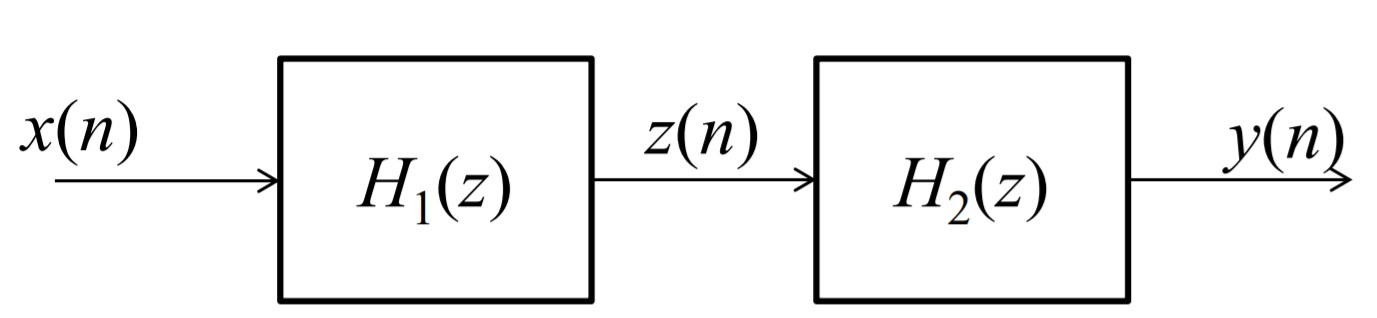
\includegraphics[width=8cm]{doublesystem}
			\caption{cascade of two systems with transfer function $H_1$ and $H_2$, input $x$, intermediate and final output respectively $z,y$.} \label{fig:z:cascade}
		\end{figure}
	
		Considering the case of a cascade of two system as shown in figure \ref{fig:z:cascade}, the output $y(n)$ of the system can be computed as
		\[ y(n) = z(n)*H_2(z) = x(n)*H_1(z) * H_2(z) \hspace{1cm} \xrightarrow{\mathcal Z} \hspace{1cm} Y(z) = X(z)H_1(z)H_2(z) \]
		From this preamble we define transfer function $H_2(z)$ as the \de{inverse} of $H_1(z)$ if and only if 
		\begin{equation}
			H_1(z)H_2(z) = 1 \qquad \Leftrightarrow \qquad H_2(z) = \frac{1}{H_1(z)}
		\end{equation}
		
		Using the stability criterion previously stated, the second system in order to be stable must have poles (namely the zeros of $H_1(z)$) that are lying within the unit circle.\\
		From this a causal and stable LTI system has an inverse that's also causal and stable if and only if all poles and zeros lie inside the unit circle and such system are called \textbf{\textit{minimum phase systems}}.
		
\section{Implementation of LTI systems: signal flow graphs}
	Considering a discrete-time causal LTI system, the numerical processing complexity heavily depends on the algorithmic implementation chosen; assuming to compute the output as the convolution of the impulse response
	\[  y(n) = \sum_{k=0}^\infty h(k) x(n-k)  \]
	then the number of multiplication and addition required linearly increases with the length of the input sequence $x(n)$ and so it's usually not a feasible solution.
	
	Considering instead to use \textbf{finite difference equations} that allows to compute the output in the form
	\begin{equation}
		y(n) = \sum_{k=0}^M \frac{b_k}{a_0} x(n-k) - \sum_{k=1}^N \frac{a_k}{a_0} y(n-k)
	\end{equation}
	the computation requires $M+N$ additions/multiplication for each computed sample (independently from the length of the input sequence $x(n)$); this is usually the preferred way to solve discrete-time systems. The last way to numerically implement such type of systems is by using the transfer function:
	\[ Y(z) = H(z)X(z) \]
	This operation is generally not profitable because it requires the computation of the Z transform ant it's successive inversion.
	
	\subsection*{Block diagrams and signal flow graphs}
		To graphically represent LTI system two equivalent methods can be used: \de{block diagrams} where \textit{blocks} (performing generic operation) are connected by arrows while the other method uses \de{signal flow graph} by having nodes adding weighted edges (the contains in themselves the multiplication); comparison between this two dual representation is shown in figure \ref{fig:z:dualrepresentationgraph}.
	
		\begin{figure}[bht]
			\centering 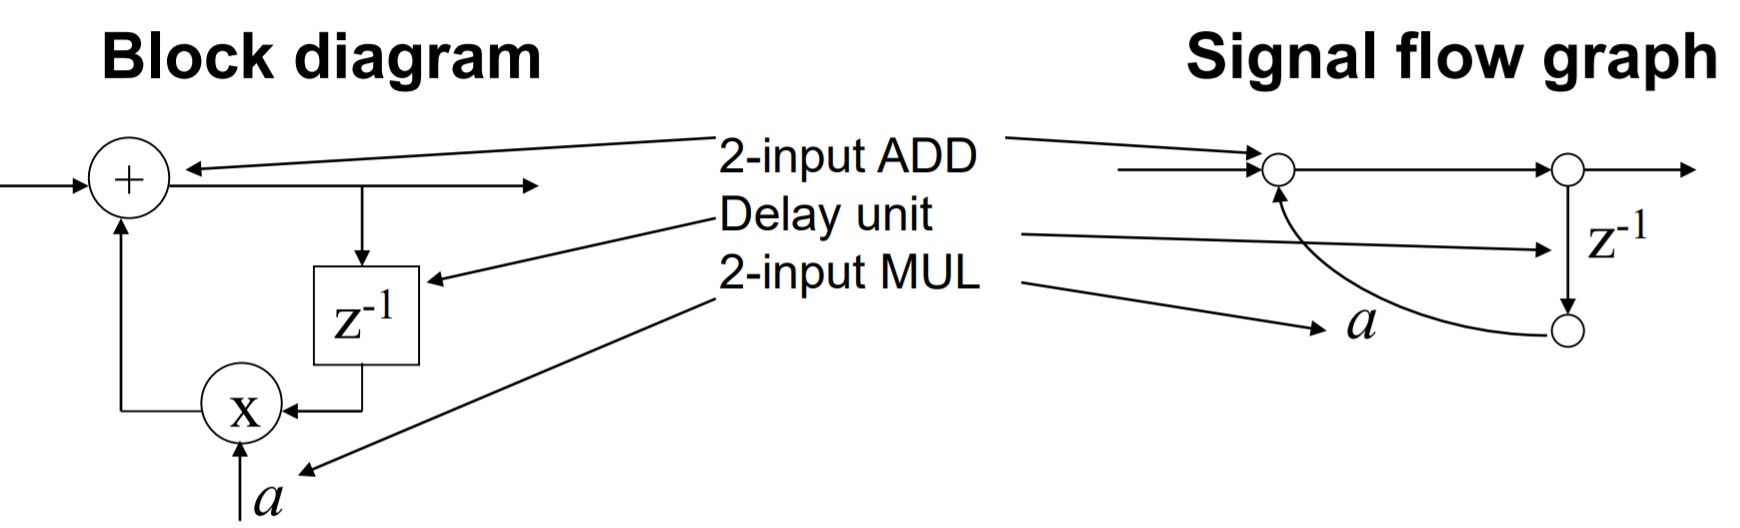
\includegraphics[width=10cm]{graphs}
			\caption{block diagram vs signal flow graph representation and correlation between the various operations performed.} \label{fig:z:dualrepresentationgraph}
		\end{figure}
	
		Such kind of description is useful in digital signal processing because it allows a \textit{good} design and modelling of the system itself before the proper hardware/software implementation. Any discrete-time transfer function can be represented as a flow graph (and using transposition property even more forms can be formulated).
		
		\paragraph{Computable graph} A signal flow graph is referred as \de{computable} if and only if it's possible to compute all the variables of the graph according to a specified order starting from given initial conditions.
		
		Considering as example the graph shown in figure \ref{fig:z:computablegraph} it's possible to define the values of all the edges considering the signals
		\begin{align*}
			w(n) & = x(n) + a \, u(n) \\ z(n) & = w(n) \\ u(n) & = z(n-1) 
		\end{align*}
		hence the output is
		\[y(n) = z(n) = x(n) + a \,y(n-1)\]		
		\begin{SCfigure}[2][bht]
			\centering 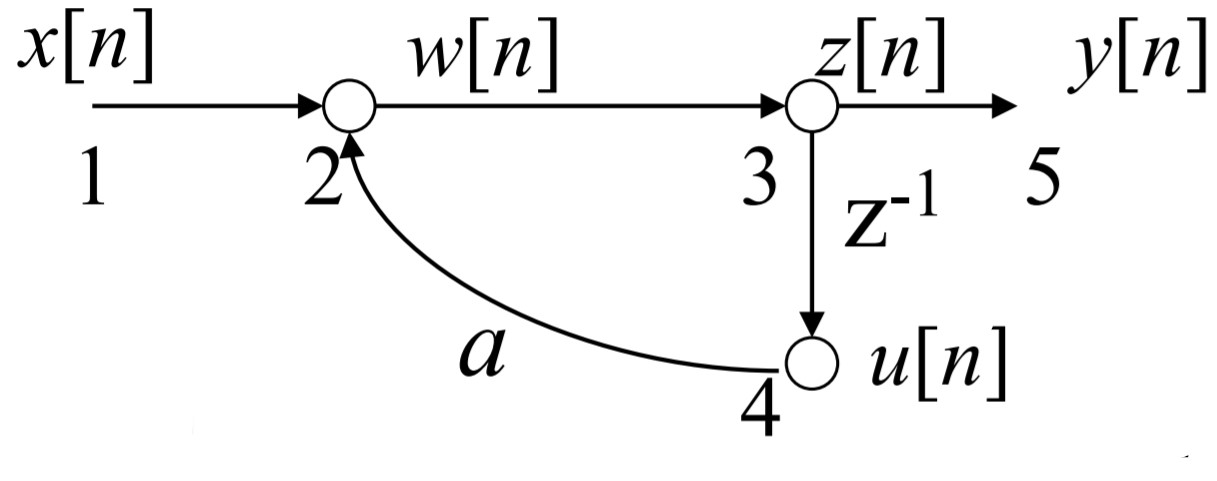
\includegraphics[width=4.5cm]{computegraph}
			\caption{example of computable flow graph.} \label{fig:z:computablegraph}
		\end{SCfigure}
		
		Considering instead the graph in figure \ref{fig:z:noncomputable}, the same analysis gives the signals
		\begin{align*}
			w(n) & = x(n) + a\,z(n) \\ z(n) & = w(n) \\ y(n) & = z(n)
		\end{align*}
		In this case it's impossible to decide whether to compute before the second node (determining $w(n)$) of the third ($z(n)$).	
		\begin{SCfigure}[2][bht]
			\centering 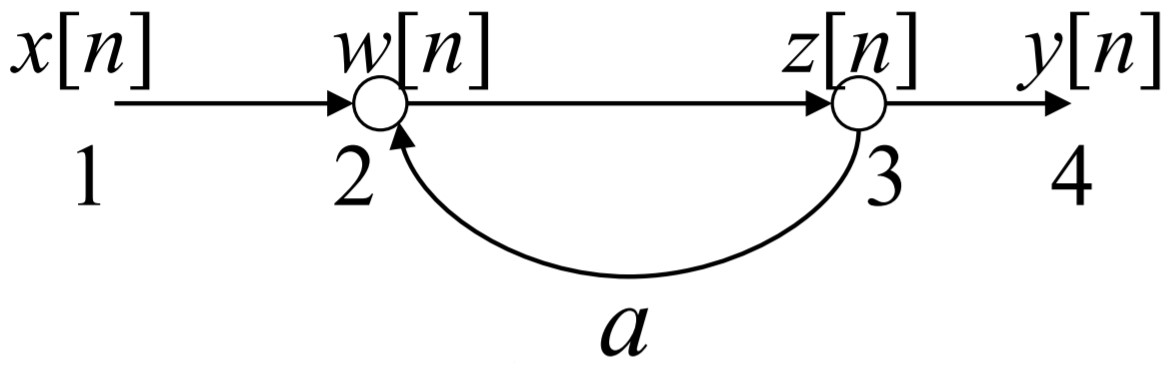
\includegraphics[width=4.5cm]{noncomputable}
			\caption{example of non-computable flow graph.} \label{fig:z:noncomputable}
		\end{SCfigure}
		
		As general \textbf{property} a signal flow graph is computable if and only if each loop in the graph contains at least one delay element.		
		
	\subsection{Direct form I and II}
		As was previously shown, discrete-time LTI systems can be described both in the discrete-time domain using the form
		\[ y(n) = \sum_{k=0}^M b_k x(n-k) - \sum_{k=1}^N a_k y(n-k) \]
		or the dual in the frequency domain
		\[ Y(z) = \dfrac{\sum_{k=0}^{M}b_k z^{-k}}{ 1+ \sum_{k=1}^{N}a_k z^{-k}} X(z) = H_{num}(z) X(z) H_{den}(z) \]
		
		Considering the transfer function $H(z) = H_{num}(z)/H_{den}(z)$ characterized by the polynomial in $z^{-1}$ for the numerator and denominator allows to write the \de{direct form I} of the associated flow graph by \textit{drawing} the \textit{ladders} as shown in figure \ref{fig:z:direct1}. Such implementation requires
		\[ M+N+1 \text{ multiplications} \qquad M+N \text{ additions} \qquad M+N\text{ delays} \]
		
		\begin{SCfigure}[2][bht]
			\centering 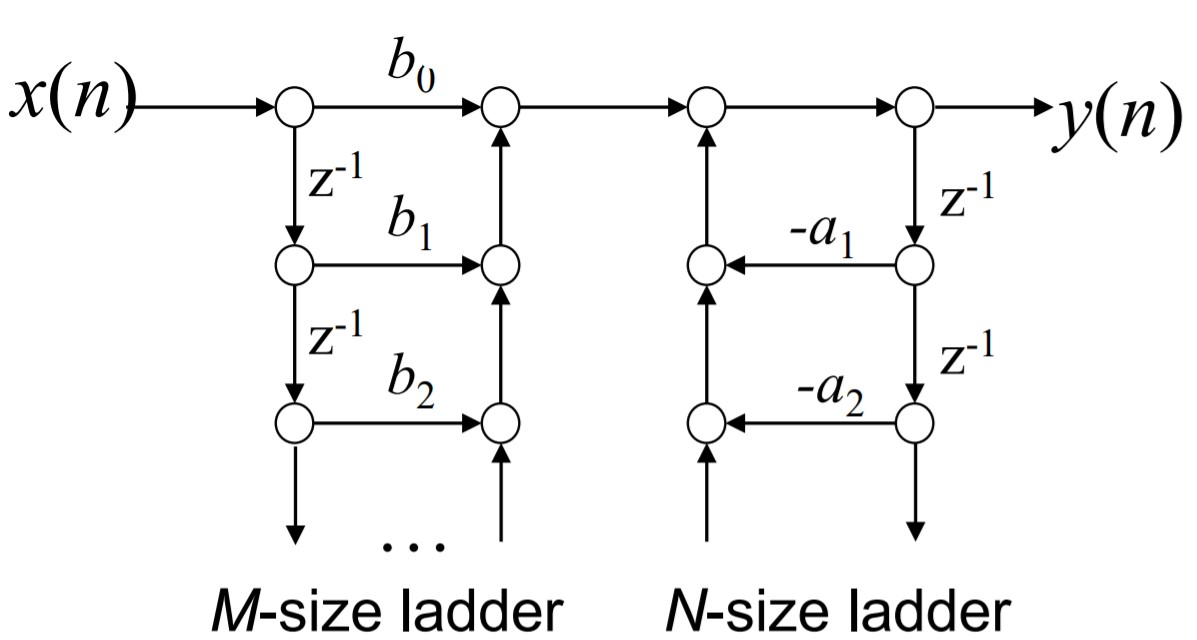
\includegraphics[width=6cm]{direct-form-1}
			\caption{first direct form flow graph representation for discrete-time systems.} \label{fig:z:direct1}
		\end{SCfigure}
	
		To reduce the computational costs of the graph computation we can consider the commutative property of the multiplication, considering so the output as $Y(z) = H_{den}(z) H_{num}(z)X(z)$; this means \textit{swapping} the ladders of the numerator/denominator of the first direct form determining so the \de{direct form II} (or \textbf{canonical}) flow graph representation. As shown in figure \ref{fig:z:direct2}, this \textit{re-arrangement} allows to reduce the delay computations reducing the numerical calculations to
		\[ M+N+1 \text{ multiplications} \qquad M+N \text{ additions} \qquad \max\{ M,N \}\text{ delays} \]
		
		\begin{SCfigure}[2][bht]
			\centering 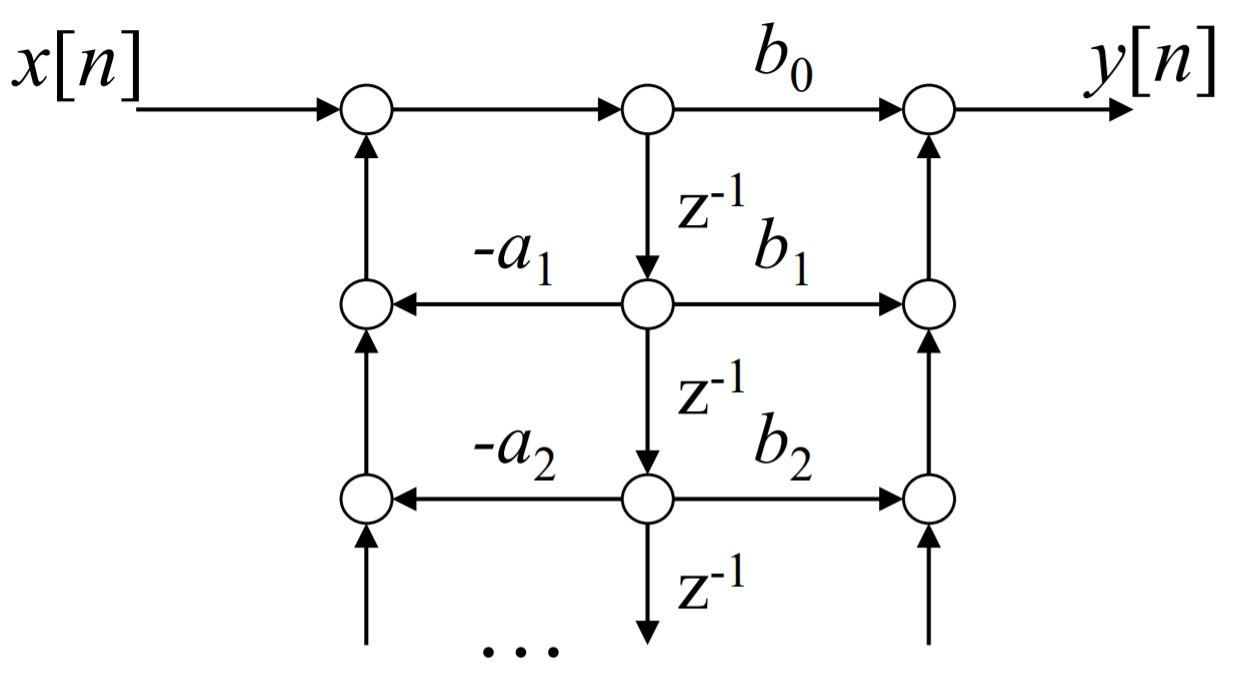
\includegraphics[width=6cm]{direct-form-2}
			\caption{second direct form flow graph representation for discrete-time systems.} \label{fig:z:direct2}
		\end{SCfigure}
		
	\subsection{Transposed form II}
		Transposing the canonical flow graph we obtain the \de{transposed form II} one as shown in figure \ref{fig:z:transposed2}; this implementation still relies on
		\[ M+N+1 \text{ multiplications} \qquad M+N \text{ additions} \qquad \max\{ M,N \}\text{ delays} \]
		but also is naturally \textit{pipelined-oriented}, meaning that is more suitable for hardware (but also software) implementation because long data-paths are broken by registers into shorter data paths.
		
		\begin{SCfigure}[2][bht]
			\centering 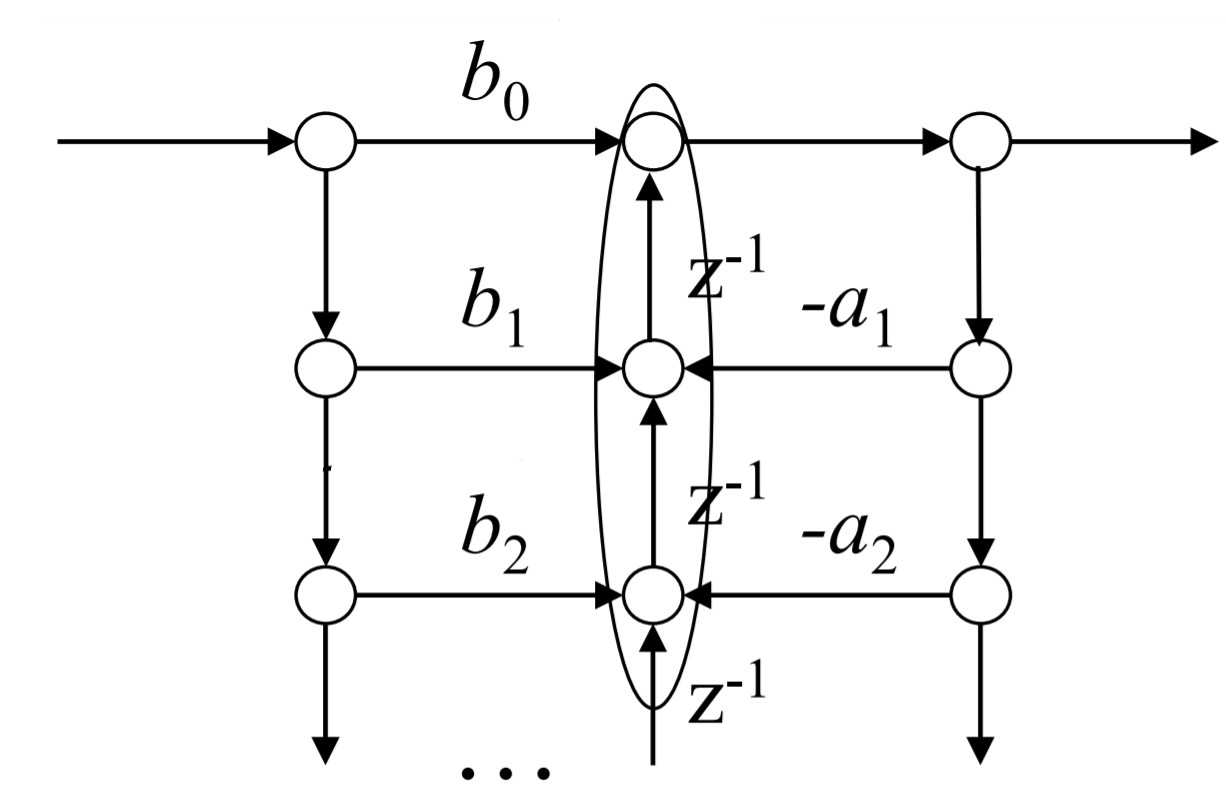
\includegraphics[width=6cm]{transposed-form-2}
			\caption{flow graph of transposed form II obtained as transosition of the canonical graph (figure \ref{fig:z:direct2}).} \label{fig:z:transposed2}
		\end{SCfigure}
		
		
		
		
		
		
		
		
		
		
		
		
		
		
		
		
		
		
		
		
		
		
		
		
		
		
	\chapter{Digital Filter Design} \label{sec:digitalfilterdesign}
	In general \de{filters} for digital signal processing are implemented in discrete-time system because, in opposition to the continuous-time one, they are easier to implement (they are in fact \textit{simple} algorithms).
	
	Given a causal discrete-time LTI system characterized by a impulse response $h(t)$, it's output to a sinusoidal input in the complex form $x(n) = A e^{j(\omega_0n+\phi_0)}$ is determined by the convolution
	\begin{equation} \label{eq:filt:shift}
	\begin{aligned} 
		y(n) & = x(n) * h(n) = \sum_{k=0}^\infty A e^{j(\omega_0(n-k)+\phi_0)}h(k) = Ae^{j\phi_0} e^{j\omega_0n} \sum_{k=0}^\infty h(k) e^{j\omega_0k} \\
		& = A e^{j(\omega_0n + \phi_0)}H\big(e^{j\omega_0}\big)
	\end{aligned}
	\end{equation}
	From this equation we can indeed see that the output of such system is still a sinusoidal function with unchanged pulsation $\omega_0$ but with a phase shift and magnitude \textit{rescalation} due to the transfer function $H$ of the system evaluated at the point $e^{j\omega_0}$ in the frequency domain. Considering the real part of the function we determine the \textit{true} output of the system as
	\[ y(n) = A \left| H\big(e^{j\omega_0}\big) \right| \cos\Big( \omega_0n + \phi_0 + \angle H\big(e^{j\omega_0}\big) \Big) \]
	where $|H(e^{j\omega})|$ is the \textbf{gain} of the system and $\angle H(e^{j\omega})$ it's \textbf{phase shift}; both parameters are evaluated for the sinusoidal pulsation $\omega_0$.	
	
	\begin{SCfigure}[2][bt]
		\centering 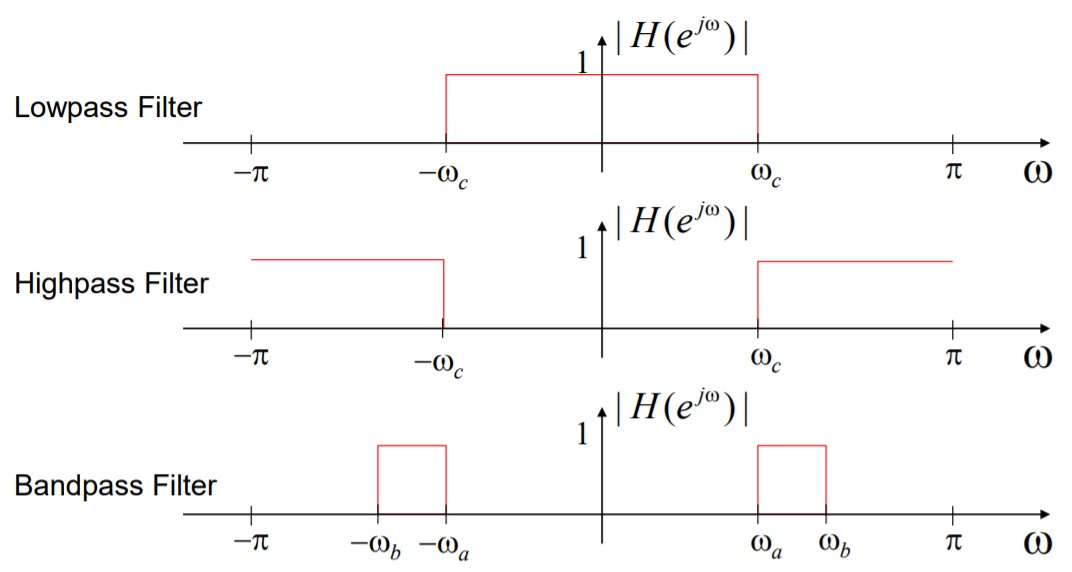
\includegraphics[width=8cm]{ideal-filters}
		\caption{examples of ideal filters in the frequency domain.}
		\label{fig:filt:idealfilter}
	\end{SCfigure}

	\paragraph{Ideal filters} Figure \ref{fig:filt:idealfilter} presents a list of the main \de{ideal filters} for discrete-time system; in particular are presented the low-pass, high-pass and band-pass filters analogous to the continuous-time ideal filters shown in section \ref{sec:conv:filters} (page \pageref{sec:conv:filters}). In practise filter with such frequency response cannot be implemented due to their \textbf{non-causality}: this kind of filters implies in fact a impulse response
	\[ h(n) \neq 0 \qquad \textrm{for } n < 0 \]
	meaning that the output should be affected by inputs that still hasn't committed.
	
	\paragraph{Low-pass filter} A low-pass filter (or any filter in general) can be practically implemented by constructing a proper window function $w(n)$ whose goal is to \textit{simulate} the spectral behaviour of the ideal counter-part. Due to the fact that they are computed on a finite number of samples $M$, the originate a distorted frequency response (respect to the ideal case) involving ripples and not-infinite slope at the cut-off frequency (as shown in figure \ref{fig:filt:windowfilter}). This ripples affect both the pass and the stop-band response due to oscillations: the pass-band gain isn't constant and the stop-band isn't univocally null.	
	
	\begin{SCfigure}[2][bht]
		\centering \includegraphics[width=5.5cm]{lpf-wind}
		\caption{spectral behaviour of low pass filter realised by appropriate windows of length $M$.}
		\label{fig:filt:windowfilter}
	\end{SCfigure}

\section{Filter specifications}
	In general the \textbf{design} of every \textbf{digital filter} derives by the design of a continuous-time low-pass filter. Acknowledged that an ideal implementation isn't feasible in real world application it's mandatory to define the following \de{design parameters} made on the assumption that the pass band gain is unitary:
	\begin{enumerate}[a)]
		\item the maximum deviation $\delta_1$ from the pass-band gain meaning that the real filter gain in the pass-band region must be bounded in the domain $[1-\delta_1,1]$;
		\item the maximum deviation $\delta_2$ from the 0 in the stop-band,  so ensuring that in the stop-band the gain is bounded in the set $[0,\delta_2]$;
		\item the transition bandwidth $\delta \omega$ defined as the difference of the minimum stop-band frequency $\omega_s$ and the maximum pass-band frequency $\omega_p$.
	\end{enumerate}
	
	The complete set of \textbf{specification parameters} $(\delta_1,\delta_2,\omega_p,\omega_s)$ can be synthesized in the concept of the \de{mask zone} (as shown in figure \ref{fig:filt:mask}), a graphical representation in the frequency domain of the zone that the frequency response must be stay out of (and complementary the region on which the transfer function can withstand).z
	
	\begin{SCfigure}[2][bht]
		\centering \includegraphics[width=7cm]{mask-zone}
		\caption{mask created to design a low pass filter.}
		\label{fig:filt:mask}
	\end{SCfigure}
	
	\paragraph{Phase distortion and group delay} Given a filter characterized by a impulse response $h(n)$ and transfer function $\four{h(n)} = H(e^{j\omega})$, the phase shift of a pure sinusoidal input function will be in general different depending on the phase of the system; using equation \ref{eq:filt:shift} we in fact have that
	\[ \angle H\big(e^{j\omega_1}\big) \neq \angle H\big(e^{j\omega_1}\big) \qquad \textrm{with } \omega_1 \neq \omega_2 \]
	For particular application phase distortion is relevant and should be minimized, and making it ideally constant through-out all the pass-band region; if this operation can't be achieved we can used the generalized concept of \de{group delay} $\tau_g$ defined as
	\begin{equation}
		\tau_g := - \frac{d\angle H \big(e^{j\omega}\big)}{d\omega}
	\end{equation}
	In the ideal case $\tau_g$ is constant with a value $\beta$ in the pass band meaning that, by integration, the \textbf{generalized group delay} is determined by an expression of the kind
	\[ \angle H\big(e^{j\omega}\big) = -\beta \omega + \alpha \hspace{2cm} \textrm{with } \alpha,\beta \in \mathds R \]
	
	\paragraph{Design techniques} Depending on the type of filter wanted, completely different approaches can be used, in particular
	\begin{itemize}
		\item to realize a IIR infinite impulse response filter the technique used is the approximation of standard analog filters; the main draw-back of this category of filters is that none of them has a linear phase response;		
		\item to realize an FIR finite impulse response filter two methods can be used: using particular window function or using algorithmic approaches based on optimization technique. This kind of filters can presents a generalized group delay.
	\end{itemize}

\section{IIR filter design}
	The design of any \de{discrete-time infinite impulse response filter} is based on the design of a well establisher \textbf{low-pass prototype} that's generated by following this steps:
	\begin{itemize}
		\item[0)] using \textit{bilinear transformations} the specification of a generic filter must be transformed in the specification of a single low-pass filter. This step is optional and has to be applied every-time we want to design a non-low-pass filter;		
		\item[1)] convert the discrete-time filter specifications $\omega_p,\omega_s$ into the dual analog $\Omega_p,\Omega_s$ for  continuous-time low-pass prototype;
		\item[2)] design the analog prototype considering some base reference; in the following pages Butterworth, Chebyshev I/II and elliptic filters are going to be presented;
		\item[3)] return to the discretized domain using the \textbf{impulse invariance} (not object of study) or the bilinear transform method;
		\item[4)] optionally if the filter object of study wasn't a low-pass filter, we have to apply the inverse transformation of step 0 in order to retrieve the desired filter.
	\end{itemize}
	
	\subsection{Finite difference method and bilinear transform}
		Observing that the variable $s$ in the Laplace domain corresponds to a differentiation in time and so for each $s$ present in the transfer function, the order of differentiation increases. This concept is valid for continuous-time systems however an analogy can be stated for discrete-time system the concept of derivation is interpreted by a numerical approximation; the simplest way to consider the derivative $y(n) = \frac{dx}{dn}$ can be obtained considering the definition
		\[ y(n) = \frac{x(n) - x(n-1)}{T} \]
		However numerically this solution is quite \textit{bad} and the \textbf{trapezoidal rule} is preferable having
		\begin{equation}
			\frac{y(n) + y(n-1)} 2 = \frac{x(n) - x(n-1)}{T}
		\end{equation}
		Applying the Z transform on such expression we have
		\[ \frac{Y(z) + z^{-1}Y(z)}{2} = \frac{X(z) - z^{-1}X(z)}{T} \]
		that determines the \textbf{Tustin}/\de{bilinear differentiation} as the transfer function
		\[\frac{Y(z)}{X(z)} = \frac 2 T \frac{1-z^{-1}}{1+z^{-1}} = s\]
		relating this numerical differentiation with the one in the Laplace domain characterized by the variable $s$; considering so the relations between the Z domain and the Laplace one determine by
		\begin{equation}
			s =  \frac 2 T \frac{1-z^{-1}}{1+z^{-1}} \hspace{1.2cm} \Leftrightarrow \hspace{1.2cm} z = \frac{1 + \frac T2s}{1-\frac T2s}
		\end{equation}
		it's possible to express the transfer function $H(z)$ of the discrete-time filter by knowing the continuous-time one $H_c(s)$ as
		\begin{equation} \label{eq:filt:bilinear}
			H(z) = H_c(s) \Big|_{s =  \frac 2 T \frac{1-z^{-1}}{1+z^{-1}}}
		\end{equation}
		This result is so used in the 3$^{rd}$ step of the digital filter design process in order to transform the analog prototype in the final desired filter. The first step based on transforming the filter specification from the discrete-time domain to the continuous one can be obtained by the bilinear transformation considering only the imaginary part $s=j\Omega$ of the Laplace variable:
		\begin{equation} \label{eq:filt:freqchange}
		\begin{aligned}
			j\Omega & = \frac 2 T \frac{1-e^{-j\omega}}{1+e^{j\omega}} = j \frac 2 T \frac{ e^{j\frac\omega2} - e^{-j\frac\omega2} }{e^{j\frac\omega2} + e^{-j\frac\omega2}} = j \frac 2 T \tan \left( \frac \omega 2 \right) \\
			\Omega & = \frac 2 T \tan \left( \frac \omega 2 \right) \\
			\omega & = \arctan \left( \frac{\Omega T}{2} \right)
		\end{aligned}
		\end{equation}
		Such transformation implies a \textbf{frequency warping}: the relation between the frequencies analog and discrete filters isn't linear but affected by a (arc)tangent function that preserves the integrity of the spectrum (no aliasing occurs because for $\Omega \rightarrow \pm\infty$ we obtain $\omega= \pm \pi$).
		
		
		
		
		
		
		
		
		
		
		
		
	\subsection{Butterworth filter}
		The \de{Butterworth filter} is one of the simplest system that can be design and is referred also as \textbf{\textit{maximally flat filter}}; the idea behind such filter is to have derivative up to $N$-th order (the \textbf{order} of the filter) that are nulls. The magnitude of such filter is in fact described by the equation
		\begin{equation} \label{eq:filt:magbutter}
			|H_c(\Omega)|^2 = \frac{1}{1 + \left(\frac{\Omega}{\Omega_c}\right)^{2N}}
		\end{equation} 
		where $\Omega_c$ is the \textbf{cut-off frequency} of the analog prototype. As shown in figure \ref{fig:filt:buttanalog}, the magnitude response is strictly monotonically decreasing and the \textbf{selectivity} (\textit{length} of the transition bandwidth) increases as the order $N$ grows.
		
		\begin{SCfigure}[2][bht]
			\centering \includegraphics[width=8cm]{butter-time}
			\caption{frequency response of the Butterworth filter with cut-off frequency $\Omega_c=1$ for various order $N$.} \label{fig:filt:buttanalog}
		\end{SCfigure}
	
		The main drawback of the Butterworth filter is that it's phase distortion is strictly non-linear in the neighbourhood of the cut-off frequency (however such effect can be neglected if we are \textit{far} from such point), as shown in the Bode plots in figure \ref{fig:filt:buttbode}.	
	
		\begin{SCfigure}[2][bht]
			\centering \includegraphics[width=5cm]{butter-bode}
			\caption{Bode plots of the response of the Butterworth filter.} \label{fig:filt:buttbode}
		\end{SCfigure}
		
		The \textit{complete} expression of the Butterworth frequency response can be obtained by expanding the full complex notation on equation \ref{eq:filt:magbutter}, obtaining
		\begin{equation}
			|H_c(\Omega)|^2 = H_c(s)\Big|_{s=j\Omega} H_c(-s)\Big|_{s=j\Omega} = \frac{1}{j\Omega + \left( -\frac{s}{\Omega_c} \right)^{2N}}
		\end{equation}
		This transfer function has no zeros (the numerator is just constant) and $2N$ poles lying on the unit circle on the complex plane of the variable $s$; discarding the \textit{unstable points} (the one having positive real parts) then the final poles for the Butterworth filter are described as:
		\begin{equation} \label{eq:filt:buttphase}
			\text{root's phases:} \hspace{2cm} \phi_k = \frac \pi 2 + \big(2k+1\big) \frac{\pi}{2N} \qquad \textrm{with } k=0,\dots, N-1
		\end{equation} 
	
		\subsubsection{Prototype design}
		When designing a Butterworth low-pass prototype no information are known a-priori regarding both the cut-off frequency $\Omega_c$ of the filter and it's order $N$; the only information known are the maximum/minimum deviation $\delta_1,\delta_2$  from the pass/stop-band gains and the related analog  frequencies $\Omega_p,\Omega_s$.\\
		In order to determine the parameters of the Butterworth filter we can impose that at the maximum pass-band frequency $\Omega_p$ the gain is at it's minimum value $1-\delta_1$, giving the expression
		\[ \frac 1 {1 + \left( \frac{\Omega_p}{\Omega_c} \right)^{2N}} = \big(1-\delta_1\big)^2 \]
		while at the minimum stop-band frequency $\Omega_s$ the allowed gain is $\delta_2$, hence
		\[ \frac 1 {1 + \left( \frac{\Omega_s}{\Omega_c} \right)^{2N}} = \delta_2^2 \]
	
		Solving the non-linear system determined by this two equations determines both the minimum order $N$ of the filter and the cut-off frequency $\Omega_c$ of the filter as
		\begin{equation} \label{eq:filt:butter}
			N = \left\lceil \frac{\ln \left( \dfrac{ \frac 1 {\delta_2^2} -1 }{\frac{1}{(1-\delta_1)^2}-1} \right)}{2 \ln \left(\dfrac{\Omega_s}{\Omega_p}\right)} \right\rceil \hspace{2cm} \Omega_c = \frac{\Omega_s}{\sqrt[2N]{\frac{1}{\delta_2^2}-1}}
		\end{equation}
		
		\begin{example}{: Butterworth low-pass filter design}
			Given the low-pass filter specification
			\[ \omega_p = 0.2\pi \qquad \omega_s = 0.3\pi \qquad \delta_1 = 0.10875 \qquad \delta_2 = 0.1778  \]
			the filter is designed considering the 3 main steps previously described, and in particular:
			\begin{enumerate}
				\item the first thing is to convert the digital filter specification into analog ones in order to build the matching prototype; in order to do so we have to consider the bilinear transform as in equation \ref{eq:filt:freqchange} where the sampling time $T$ is arbitrarily chosen to be 1, and so
				\[ \Omega_p = 2\tan\left( \frac{\omega_p}{2} \right) =0.6498 rad/s \qquad \Omega_s = 2\tan \left( \frac{\omega_s}{2} \right) = 1.019 rad/s \]
				
				\item with the specification of the low-pass prototype stated it's possible to use equation \ref{eq:filt:butter} to determine the minimum order $N$ of the filter as
				\[ N = \left\lceil \frac{\ln \left( \dfrac{\frac{1}{0.1778^2}-1}{\frac 1{0.89^2}-1} \right) }{2 \ln\left(\dfrac{1.019}{0.6498}\right)} \right\rceil = \big\lceil 5.3 \big\rceil = 6 \] 
				and so the cut-off frequency
				\[ \Omega_c = \frac{1.019}{\sqrt[12]{\frac{1}{0.1778^2}-1}} = 0.7662 rad/s \]
				With this parameters defined it's possible to compute the roots of the filter as $s_k = \Omega_c \big(\cos\phi_k \pm j \sin \phi_k\big)$ where $\phi_k$ was defined in equation \ref{eq:filt:buttphase} and we obtain
				\[ s_{0,5} = -0.198 \pm j 0.74 \qquad s_{1,4} = -0.54 \pm j 0.54 \qquad s_{2,3} = -0.74 \pm j 0.198 \] 
				Considering the expansion $(s-s_k)(s-s_k^*) = s^2- 2s\Re{s_k} + |s_k|^2$ and that $|s_k|= \Omega_c$ then the formulation in the Laplace domain of the low-pass prototype is
				\[ H_c(s) = \frac{H_0}{\prod_{k=0}^{N-1} (s-s_k) } = \frac{0.202}{ (s^2 + 0.397s + 0.587)(s^2+1.085s+0.587)(s^2+1.185s + 0.587) } \]
				where $\Omega_0$ was determined as $\prod_{k=0}^{5} s_k = \Omega_c^2 = 0.202$.
				
				\item using now the bilinear transform (equation \ref{eq:filt:bilinear}) it's possible to re-convert the analog prototype  (in the Laplace domain) onto the corresponding discrete-time low-pass filter; considering that each complex root is transformed as
				\[ s^2 + \alpha_k s + \beta_k\Big|_{s =  \frac 2 T \frac{1-z^{-1}}{1+z^{-1}}} = \frac{1- A_k z^{-1} + B_kz^{-2}}{C_k \big(1+z^{-1}\big)^2} \]
				where
				\[ A_k = \frac{8-2\beta_k}{4+2\alpha_k + \beta_k} \qquad B_k = \frac{4-2\alpha_k + \beta_k}{4 + 2\alpha_k +\beta_k} \qquad C_k = \frac 1 {4+2\alpha_k + \beta_k} \]
				With that said the transfer function so becomes
				\begin{align*}
					H(z) & = \frac{\big(1+z^{-1}\big)^6 C_0C_1C_2 H_0}{ \big(1 - A_0 z^{-1} + B_0z^{-2}\big) \big(1 - A_1 z^{-1} + B_1z^{-2}\big) \big(1 - A_2 z^{-1} + B_2z^{-2}\big) } \\
					& = \frac{\big(1+z^{-1}\big)^6 0.186\cdot 0.148\cdot 0.144 \cdot 0.2022}{ \big(1 - 1.268 z^{-1} + 0.705z^{-2}\big) \big(1 - 1.012 z^{-1} + 0.36z^{-2}\big) \big(1 - 0.981 z^{-1} + 0.319z^{-2}\big) }
				\end{align*}
				
				
				
				
			\end{enumerate}
		\end{example}
		
	\subsection{Chebyshev type I}
		The \de{Chebyshev} of filter of the \de{first type} presents one more additional parameter: the \textbf{maximum ripple amplitude} $\varepsilon$ that determines the magnitude response of the form
		\begin{equation} \label{eq:filt:cheby1}
			\big|H_c(\Omega)\big|^2 = \frac{1}{1 + \varepsilon^2 P_N^2 \big(\Omega/\Omega_c\big)}
		\end{equation}
		where $P_N(x)$ is the \textbf{Chebyshev polynomial} of order $N$ formally defined as $P_N(x) = \cos\big(N\arccos x\big)$; expanding it's definition and making some analytical simplification we have
		\[ P_0(x) = 1 \qquad P_1(x) = x \qquad P_2(x) = 2x^2-1 \qquad P_3(x) = 4x^3-3x \]
		We can see so that, starting from the first 2 polynomials, the other can be computed considering the recursive definition $P_N(x) = 2x P_{N-1}(x) - P_{N-2}(x)$.
		
		\begin{SCfigure}[2][bt]
			\centering \includegraphics[width=5cm]{cheby-1}
			\caption{Bode plots of the response of the Chebyshev type I filter.} \label{fig:filt:cheby-1bode}
		\end{SCfigure}
		
		As shown in figure \ref{fig:filt:cheby-1bode} this kind of filter is characterized by an \textbf{equi-ripple} behaviour (the ripples have the same \textit{amplitude}) in the pass-band with a ripple amplitude equal to $\varepsilon$ while no ripples are present in the stop-band; this phenomena leads to a severe phase distortion in the same region but this kind of filter, for the same order $N$, has a \textit{sharper} transition bandwidth meaning that's more selective.
		
		By doing a full analysis of equation \ref{eq:filt:cheby1} it can be observed that the function still has no zeros but have $2N$ poles lying on an ellipse in the complex plane with a major diameter belonging to the imaginary axis ranging from $-j$ to $j$. To position of the poles is defined by equation
		\begin{equation}
			s_k = r_1 \cos\phi_k + j r_2 \sin\phi_k \hspace{2cm} k = 0,\dots, N-1
		\end{equation}
		where
		\[ r_1 = \frac 1 2 \left( \sqrt[N]\alpha - \sqrt[N]{\frac 1 \alpha} \right) \qquad r_2 = \frac 1 2 \left( \sqrt[N]\alpha + \sqrt[N]{\frac 1 \alpha} \right) \qquad \alpha = \frac 1 \varepsilon + \sqrt{1 + \frac{1}{\varepsilon^2}} \qquad \phi_k = \frac \pi 2 + (2k+1) \frac \pi {2N} \]
	
		\subsubsection{Prototype design}
		In the design of the prototype the first step is to relate the maximum deviation $\delta_1$ in the pass-band region with the maximum ripple amplitude parameter $\varepsilon$ that's so determined by the expression
		\begin{equation}
			1 - \delta_1 = \frac{1}{\sqrt{1+\varepsilon^2}} \hspace{1.2cm} \Rightarrow \hspace{1.2cm} \varepsilon = \sqrt{\frac 1 {\big(1-\delta_1\big)^2} - 1}
		\end{equation}
		By applying similar boundary conditions stated on the prototype design of the Butterworth filter we can obtain the minimum order $N$ of the filter as
		\begin{equation}
			N = \left\lceil \frac{\ln\left( \dfrac{\sqrt{1-\delta_2^2} + \sqrt{1-\delta_2^2(1+\varepsilon^2)}}{\varepsilon\delta_2} \right)}{\ln\left( \dfrac{\Omega_s}{\Omega_p} + \sqrt{\left( \dfrac{\Omega_s}{\Omega_p} \right)^2 - 1} \right)} \right\rceil
		\end{equation}
		In this case the cut-off frequency of the filter coincides with the maximum pass-band frequency, so $\Omega_c=  \Omega_p$.


\section{FIR filter design}
	The design of \de{finite impulse response} FIR filters for discrete time system can be principally made in two ways:
	\begin{itemize}
		\item by constructing a proper window whose spectra effect is similar to the ideal case;
		\item by using algorithms based on optimization in the frequency domain; usually this filter implementation (for the same length $L$ of the signal to filter) is more selective respect to the window method.
	\end{itemize}
	Usually this kind of filters are explicitly design to have a (generalized) \textbf{linear phase} response.

	\subsection{Types of linear phase systems}
		Considering filters designed by constructing a proper finite impulse response, we can classify such system in 4 types depending on the length of the impulse response $h(n)$ and it's symmetry, in particular we have 4 types:
		\begin{enumerate}[I)]
			\item $h(n) = h(M-n)$ with $M$ even;
			\item $h(n) = h(M-n)$ with $M$ odd;
			\item $h(n) = - h(M-n)$ with $M$ even;
			\item $h(n) = - h(M-n)$ with $M$ odd;
		\end{enumerate}
		The first two types are so characterized by an axe of symmetry positioned at $M/2$ (note that for the type I such axis lies on a sample, while for type II it passes in the middle of two \textit{steps}), while for the last two there's a point symmetry (still at $M/2$).
		
		\paragraph{Linear phase proof} Considering a type I FIR filter, it's possible to prove it's linear phase; known it's impulse response
		\[ h(n) = \sum_{k=0}^M b_k \delta(n-k) \hspace{2cm} \textrm{where } b_k = b_{M-k} \]
		then it's \dtft can be computed as
		\begin{align*}
			H\big(e^{j\omega}\big) & = \sum_{k=0}^M b_k e^{-j\omega k} = b_{M/2} e^{-j\omega \frac M2} + \sum_{k=0}^{\frac M2 -1} b_k \left( e^{-j\omega k} + e^{-j\omega(M-k)} \right) \\
			& = b_{M/2} e^{-j\omega \frac M2} + 2 e^{-j\omega \frac M2} \sum_{k=0}^{\frac M2 -1} b_k \left( \frac{e^{j\omega \left(\frac M2 - k\right)} + e^{-j\omega \left(\frac M2 - k\right)} }{2} \right)
		\end{align*}
		Knowing the Euler relation $\frac{e^{jx} + e^{-jx}}{2} = \cos x$ and performing the change of variable $m = \frac M 2 - k$ it possible to rewrite such expression as
		\[ H\big(e^{j\omega}\big) = e^{-j\omega \frac M2} \sum_{m=0}^{\frac M2} c_m \cos (m \omega) \]
		where
		\[ c_0 = b_{M/2} \hspace{2cm} c_m = 2 b_{\frac M2 -m} \quad \textrm{with } m = 1,\dots, \frac M2 \]
		Considering that the summation of cosines determines a purely real and even function, then the transfer function of the filter can be regarded as
		\begin{equation}
			H\big(e^{j\omega}\big) = e^{-j\omega \frac M2} A_e(\omega)
		\end{equation}
		where $A_e$ is a real and even function in the discrete frequencies $\omega$; the phase of such system is so
		\[ \theta(\omega) = \omega \frac M 2 + \angle A_e(\omega) \qquad \textrm{where } \angle A_e(\omega) = \begin{cases}
			0 \qquad & A_e(\omega) \geq 0 \\
			\pi \qquad & A_e(\omega) < 0 \\
		\end{cases} \]
	
		\paragraph{Location of the zeros} Considering the symmetric case (type I and II linear phase systems) we have that
		\[ h(n) = h(M-n) \qquad \xrightarrow{\mathcal Z} \qquad H(z) = z^{-M} H(z^{-1}) \]
		We can so observe that
		\begin{itemize}
			\item if $z_0$ is a real zero, then also $1/z_0$ is a zero of the transfer function and so zeros always comes in pairs;
			\item if $h(n)$ is real evaluated and $z_0$ is more generally a complex zero, then also $z_0^*$, $1/z_0$ and $1/z_0^*$ are also zeros (complex-valued zeros come in quadruples);
			\item if a zero is on the unit circle then it's reciprocal equates it's conjugate (the quadruple becomes a a pair); moreover if $z\pm 1$ then the reciprocal and the conjugate coincides.
		\end{itemize}
		Note that if $z=-1$ and $M$ is odd, then this means $H(-1) = (-1)^{-M}H(-1)$ hence $H(-1)=0$: type II filters must always have a zero in $z=-1$.
		
		The same considerations holds for type III and IV linear phase systems, but the Z transform applied on such filters is in the form
		\[ H(z) = - z^{-M} H(z^{-1}) \]
		\begin{enumerate}
			\item if $z=-1$ and $M$ is even, then $H(-1) = -(-1)^{-M} H(-1)$ where so $H(-1) = 0$ meaning that type III system must always have a zero in $z=-1$;
			\item considering instead the case of $z=1$ independently by the value $M$ we obtain that $H(1) = 0$ and so any type III and IV system must have a zero in $z=1$.
		\end{enumerate}
	
	\subsection{Design: windowing method}
		Given the ideal frequency response $H_{id}(e^{j\omega})$ of the low pass filter defined as
		\[ H_{id} \big(e^{j\omega}\big) = \begin{cases}
			1 \qquad & |\omega| \leq \omega_c \\0 & \omega_c < |\omega| < \pi
		\end{cases} \]
		the ideal non-causal impulse response of such filter is described by the function
		\[ h_{id}(n) = \begin{cases}
			1 & n = 0\\
			\frac{\sin(\omega_cn)}{\pi n} \qquad & n = \pm 1,\pm 2,\pm 3,\dots
		\end{cases} \]
		\begin{note}
			this \textit{cardinal sine-look-like} sequence is obtained by applying the inverse Fourier transform on the rectangular spectrum as was computed in page \pageref{eq:four:rectangularinvers}, equation \ref{eq:four:rectangularinvers}.
		\end{note}
		The basic idea to implement such filter is so to use a finite length $M$ signal (truncating to a certain level the ideal impulse response) and delaying him in order to make him causal and so
		\begin{equation}
			h(n) = \begin{cases}
				h_{id}\left(n-\frac M2\right) \qquad & n = 0,\dots,M \\0 & \textrm{otherwise}
			\end{cases}
		\end{equation}
		The so determined real spectral behaviour can so be computed convolving the ideal low-pass transform with the one of the rectangular window of $M$ samples, hence
		\begin{equation}
			H\big(e^{j\omega}\big) = e^{-j\omega \frac M2} H_{id}\big(e^{j\omega}\big)  W \big(e^{j\omega}\big) = \frac{e^{-j\omega \frac M2}}{2\pi} \int_{-\pi}^{\pi} H_{id}\big(e^{j\theta}\big) \frac{ \sin \left( \frac{(\omega-\theta)(M+1)}{2} \right)  }{\sin \left( \frac{\omega - \theta}{2} \right)}\, d\theta
		\end{equation}
		
		\begin{SCfigure}[2][b!t]
			\centering \includegraphics[width=5cm]{windowfilter}
			\caption{ideal vs real frequency response of a FIR  digital low-pass filter obtained using the windowing method.} \label{fig:filt:windowlowpass}
		\end{SCfigure}
		
		As it can be seen in figure \ref{fig:filt:windowlowpass}, the impulse response truncation determines ripples causing approximation errors (due to the windowing) that cannot be handled (we cannot influence neither the ripple amplitude $\delta_1,\delta_2$ nor the selectivity); having a symmetric impulse response we obtain a type I or II linear phase system. This approach can be used not only for low-pass filters but for any type of LTI discrete-time system.
	
		In general increasing the filter length $M$ improves the selectivity, but the approximation errors remains unchanged; as $M$ grows the group delay and the computational cost also increase.
		
		\paragraph{Design steps} In order to design a FIR filter based on the windowing method the following procedure can be used:
		\begin{enumerate}
			\item compute the ideal impulse response $h_{id}(n)$ of the system whose transform is the associated ideal filter $H_{id}(e^{j\omega})$;
			
			\item given the filter specification (such $\delta,\omega_p,\omega_s$) chose the simplest window (considering as example the one described in table \ref{tab:dft:windowfunctions}, page \pageref{tab:dft:windowfunctions}) function such that $\varepsilon \leq 20 \log_{10} \delta$ where $\varepsilon$ is the maximum ripple amplitude;
			
			\item set  $M$ so that $\omega_s-\omega_p = \Delta \omega \geq \Delta \omega_m$ where $\Delta \omega_m$ is the main-lobe width of the chosen window;
			
			\item compute the coefficient of $w(n)$ for $n=0,\dots,M$;
			\item compute the impulse response $h(n) = h_{id}\left( n - \frac M2\right) w(n)$;
			\item compute the frequency response $H(e^{j\omega})$ of $h(n)$ and check the compliance with specifications.			
		\end{enumerate}
		If necessary start a iterative \textit{trial\&error} approach by tweaking the window length $M$ to find the proper transfer function.
	
	\subsection{Design: algorithmic method}
		Finite impulse response discrete time system can be numerically determined using optimization techniques; given the fixed ideal frequency response $H_{id}(e^{j\omega})$ and the \textit{real} $H(e^{j\omega})$ that's parametric, using numerical minimization algorithms is possible to search for parameters that minimize the maximum error, solving the problem
		\[ \textrm{minimize } \quad \Big| H\big(e^{j\omega}\big) - H_{id} \big(e^{j\omega}\big) \Big| \]
		or the norm of the error
		\[ \textrm{minimize } \quad \Big\| H\big(e^{j\omega}\big) - H_{id} \big(e^{j\omega}\big) \Big\| \]
		The minimization is so performed on a filter with a predefined length $N$ of the impulse response and such kind of problem are mathematically proven to always have a unique solution.
		
		
		
		
		
	\section{Examples}
		\begin{example}{: IIR filter design}
			The goal is to design a Butterworth discrete-time low pass filter with specifications:
			\begin{itemize}
				\item magnitude ripple of no more than $0.2dB$ for $|\omega|\leq \frac \pi 6$;
				\item stop-band attenuation of at least $25dB$ for $|\omega| \geq 0.45\pi$.
			\end{itemize}
			To solve this problem:
			\begin{enumerate}
				\item firstly we have to determine the specification of the filter in the linear domain; considering the magnitude ripple we obtain the maximum deviation $\delta_1$ as
				\begin{align*}
					20 \log_{10}(1-\delta_1) = -0.2 \qquad \Rightarrow \qquad \delta_1 & = 1 - 10^{-\frac{0.2}{20}} = 0.0227 \\
					1-\delta_1 &= 0.977
				\end{align*}
				while for the minimum deviation
				\[ 20\log_{10}\delta_2 = - 25 \qquad \Rightarrow \qquad \delta_2 = 10^{-\frac{25}{20}} = 0.056 \]
				Assuming a sampling period $T=1$, the warped frequency for the continuous-time prototype obtained by equation \ref{eq:filt:freqchange} are
				\[ \Omega_p = 2 \tan\left( \frac{\pi/6}2 \right) = 0.536 rad/s \qquad \Omega_s = 2 \tan\left( \frac{0.45\pi}{2} \right) = 1.708 rad/s  \]
				
				\item with the specification converted for the low-pass prototype, using equation \ref{eq:filt:butter} it's possible to compute the minimum order $N$ of the system 
				\[ N = \left\lceil \frac{\ln \left( \dfrac{ \frac 1 {0.056^2} -1 }{\frac{1}{0.977^2}-1} \right)}{2 \ln \left(\dfrac{1.708}{0.536}\right)} \right\rceil = \big\lceil   3.8 \big\rceil = 4\]
				and so the cut-off frequency
				\[ \Omega_c = \frac{1.708}{\sqrt[8]{\frac{1}{0.056^2}-1}} = 0.831 rad/s \]
				The poles of the transfer function are so characterized by the formulation $s_k = \Omega_c\big(\cos\phi_k \pm k \sin\phi_k\big)$ where $\phi_k = \frac \pi 2 + (2k+1)\frac{\pi}{2N}$ and so the poles are
				\[ s_{0,3} = -0.318 \pm j0.768 \hspace{1.5cm} s_{1,2} = -0.768 \pm j 0.318 \]
				Knowing that $(s-s_k)(s-s_k^*) = s^2 -2s\Re{s_k} + |s_k|^2$ and that $H_0 = \Omega_c^4 = 0.831^4 = 0.477$ we have the following transfer function:
				\[ H_c(s) = \frac{0.477}{(s^2 + 0.636s +0.69)(s^2 + 1.536s + 0.69)} \]
				
				\item for transform the continuous-time prototype in the discrete-time filter we have to apply the bilinear transform (equation \ref{eq:filt:bilinear}); knowing that
				\[ s^2 + \alpha_k s_k +\beta_k\Big|_{s=\frac 2 T\frac{1-z^{-1}}{1+z^{-1}}} = \frac{1 + A_kz^{-1} + B_k z^{-2}}{C_k(1-z^{-1})^2} \]
				where
				\[ A_k = \frac{2\beta_kT  - 8}{4+2\alpha_kT + \beta_kT} \qquad  B_k = \frac{4 - 2\alpha_k T + \beta_k T}{4+2\alpha_kT + \beta_kT} \qquad C_k = \frac{T^2}{4+2\alpha_kT + \beta_kT} \]
				then the discrete-time filter's transfer function is
				\begin{align*}
					H(z) & = \frac{H_0(1-z^{-1})^4 C_0C_1}{\big(1 + A_0z^{-1} + B_0z^{-2}\big) \big(1 + A_1z^{-1} + B_1z^{-2}\big) } \\
					& = \frac{0.477 \cdot 0.168 \cdot 0.129 (1-z^{-1})^4}{\big(1 - 1.11z^{-1} + 0.573z^{-2}\big) \big(1 - 0.853z^{-1} + 0.208z^{-2}\big) }\\
					& = \frac{ 0.0103 (1-z^{-1})^4 }{ 1 - 1.963z^{-1} - 1.727 z^{-2} - 0.719 z^{-3} +0.119 z^{-4}  }
				\end{align*}
			\end{enumerate}
			If instead we would have considered a Chebyshev filter of the first type the minimum order required for the filter is lower than the Butterworth filter due to it's higher selectivity; determined the maximum amplitude ripple
			\[ \varepsilon = \sqrt{\frac{1}{0.977^2}-1} = 0.218 \]
			the minimum order of the filter is computed as
			\[ N = \left\lceil \frac{ \ln\left( \dfrac{\sqrt{1-0.056^2} + \sqrt{1-0.056^2(1+0.218^2)} }{0.281\cdot 0.056} \right) }{\ln \left( \dfrac{1.708}{0.536} + \sqrt{\left( \dfrac{1.708}{0.536} \right)^2-1} \right)} \right\rceil = \big\lceil 2.79 \big\rceil = 3 \]
			
		\end{example}
	
	
	
	
	
	\backmatter
	
	\chapter{Fundamentals of probability and statistics}
\section*{Probability}
	Considering an experiment with random outcomes, a \textbf{event} is defined \textit{as a set of the outcomes of the experiment}, so an event occurs if the outcome of the experiment in one of the element of the set itself. By this concept we can define the \textbf{probability} $\prob{A}$ of the event $A$ as a measure that always satisfies the \textbf{three axioms of probability}:
	\begin{enumerate}
		\item $\prob{A} \geq 0$;
		\item $\prob S = 1$  if $S$ is the sure event;
		\item if two events $A,B$ such that $A \cap B = \emptyset$, or in other word they are \textit{mutually exclusive}, than $\prob{A \cup B} = \prob{A+B} = \prob A + \prob B$.
	\end{enumerate} 

	As a consequence of the last axiom, by defining $\overline A$ the \textbf{complementary event} of $A$, the respective probability is defined as $\prob{\overline A} = 1 - \prob A \leq 1$. In particular the probability of the impossible event (so $\overline S$), expressed by the empty set $\emptyset$, is evaluated as $\prob\emptyset = 0$. Any possible event is a subset of the sure event.
	
	There are usually two different views of probability:
	\begin{itemize}
		\item the \textbf{frequentist} interpretation for which the probability of something corresponds to what fraction of the time it happens \textit{"in the long run"};
		\item the \textbf{Bayesian} interpretation instead considers the probability of something corresponds to how likely we \textit{"think"} it is to happen.
	\end{itemize}
	The \textbf{relative frequency} is a non-rigorous way to introduce the concept of probability with is widely used in engineering system. Considering for example the experiment of tossing a coin (which the associated event are a head $C$ o a tail $\overline C$) and extracting a red/black card from a card deck (so the events are $R$ for the red card and $\overline R$ for the black one). At this point we can describe the sure event as the sum of all the possible outcomes of these experiment, so
	\[ S = \big\{ CR, C\overline R, \overline C R, \overline C \overline R \big\}\]
	After $n$ experiments it is possible to calculate the relative frequency $f(\cdot)$ of a event simply by dividing the number of outcomes $n_i$ in that specific set respect to $n$ itself:
	\[ f\big( CR \big) = \frac{n_1}{n} \qquad f\big( C \overline R \big) = \frac{n_2}{n} \qquad f\big( \overline CR \big) = \frac{n_3}{n} \qquad f\big( \overline C \overline R \big) = \frac{n_4}{n} \qquad  \] 
	
	From an empirical definition we can calculate the probability of tossing a head \textbf{or} extracting a red card by summing the probabilities of the mutually exclusive events that satisfies at least one of the mentioned requisites, so
	\[ f\big(C+R\big) = F \big( CR\big) + f\big(C \overline R\big) + f\big(\overline C R\big) = \frac{n_1 + n_2 + n_3}{n}\]
	Considering that the probability of tossing a head and the probability of extracting a red card are described by the equations
	\[ f\big(C\big) = f\big(CR\big) + f\big(C\overline R\big) = \frac{n_1+n_2}{n} \qquad f\big(R\big) = f\big(CR\big) + f\big(\overline C R\big) = \frac{n_1+n_3}{n} \]
	it's also possible to notice that
	\[ f\big(C+R\big) = \frac{n_1+n_2+n_3 + n_1 - n_1}{n} = f\big(C\big) + f\big(R\big) - f\big(CR\big)\]
	This relation can also be expressed only using the third axiom of probability and so $\prob{C\cup R} = \prob C + \prob R - \prob{C\cap R}$.
	\vspace{3mm}
	
	In general the probability of an event can be effected by an \textit{a-priori} knowledge of some result of the experiment; using the same example as before we can evaluate the probability $f\big(C|R\big)$ of tossing a head knowing that the event $R$ (red card extracted) has been already verified by using the following rule:
	\[ f\big(C|R\big) = \frac{n_1}{n_1+n_3} = \frac{n_1}{n} \frac{n}{n_1+n_3} = \frac{f(CR)}{f(R)} \]
	Similarly we can define the relative frequency $f\big(R|C\big)$ of $R$ knowing $C$ as $f\big(CR\big)/f\big(C\big)$; using the axiom of probability we can define the \textbf{conditional probability} as
	\[ \prob{C|R} = \frac{\prob{C\cap R}}{\prob R}\]
	By inverting this relation it's possible to write the probability of a red card and a head toss, and so
	\[ \prob{C \cap R} = \prob{C|R} \prob{R} = \prob{R|C} \prob C\]
	As consequence if $C$ and $R$ are two statistically independent events, the conditional probability $\prob{C|R}$ corresponds only to the events associated to a head coin toss, and so
	\[ \prob{C\cap R} = \prob C \prob R \]
	
	In general given two events $A,B$, as expressed before their conditional probability is described by the equation $\prob{A \cup B} = \prob{A|B} \prob B = \prob{B|A} \prob A$. By manipulating this relation it's possible to describe the conditional probability $A|B$ in relation to the other conditional probability $B|A$ by simply doing
	\[\prob{A|B} = \prob{B|A} \frac{\prob A}{\prob B} \]
	So given $n$ disjoint events $A_i$ (with $i$ that goes from 1 to $n$) it's possible to express the conditional probability $A_i|B$ of one event in respect to $B$ by using the \textbf{Bayes theorem} which states that
	\[ \prob{A_i|B}  = \prob{B|A_i} \frac{\prob{A_i}}{\prob B} =  \frac{\prob{B|A_i} \prob{A_i}}{\sum_{j=1}^n \prob{B|A_j}\prob{A_j}} \]
	In respect to this theorem we can see three main component:
	\begin{itemize}
		\item $\prob {A_i}$ is the \textit{prior probability} of the event $A_i$;
		\item $\prob{B|A_i}$ is the \textit{likelihood} of $B$ given $A_i$, so it's a measure of how likely $B$ happens when $A_i$ also happens;
		\item $\prob{A_i|B}$ is the \textit{posterior probability} of $A_i$ given $B$ (the probability of $A_i$ knowing that $B$ has actually happened).
	\end{itemize}

\section*{Random variables}
	In the majority of the engineering cases the variables are not described by set of events but with numbers. In general a \textbf{random variable} is a real-valued function that assumes a certain value according to the outcome of a certain random experiment.
	
	To a formal level the random variables maps the set containing all the possible outcomes of a certain experiments, the so called \textit{event/sample space} $\Omega$ (that can be continuous, like $\mathds R$, or discrete, like $\mathds Z$) to the space of numbers. In practise $\forall \omega \in \Omega$ we get that the mapped value $x(\omega)$ is an element of the the arriving set (like a number).	
	\begin{SCfigure}[1.5][bht]
		\includegraphics[width=5cm]{randomvariables}
		\caption{example of a random variable being mapped from a sample space $\Omega$ to a continuous set of the real number.}
	\end{SCfigure}
	
	To completely describe a random variable it's necessary to use a probabilistic description, in particular by using the so called \textbf{probability density function} (pdf) that can calculate the probability of a random variable $x$ at a certain value $x=a$ by the formula
	\[ p(a) = \lim_{\delta_a \rightarrow 0} \frac{\prob{a-\delta_a < x \leq a}}{\delta_a} \geq 0 \]
	This expression resembles a derivative: this function can in fact be integrated between two points in order to get the probability of having a random variables inside that range
	\[ \prob{a< x \leq b} = \int_a ^b p(x)\, dx \]
	From the probability density function it can be derived the \textbf{cumulative distribution function} (cdf) that describes the probability of having a random variable $x$ with value less or ugual to $b$:
	\[ P(b) = \prob{x\leq b} = \int_{-\infty}^b p(x)\, dx\]
	
	The pdf associated to a random variable, in order to satisfy the second axiom of probability, must require that
	\[ \prob{x\leq \infty} = \int_{-\infty}^\infty p(x)\, dx = P(\infty) = 1\] 
	\vspace{3mm}
	
	Usually all the probability density functions for continuous random variables can be expressed as a \textit{known distribution} by re-shaping the pdf as
	\[ p(x) = \frac{1}{c\, N(s)} p\left(\frac{x-l}{c}\right)\]
	where $l$ is the \textit{location parameter} (that has the role to translate the pdf), $c$ is the \textit{scale parameter} (associated to a expansion/contraction) and $s$ is a \textit{shape parameter} that governs the shape of the pdf and that define the normalising function $N(s)$.\\
	Examples of known probability density functions is the \textbf{uniform} one; in this case the random variable $x$ comparable to this distribution in the range $[a,b]$ is written as $x\backsim \mathcal U(a,b)$ and in particular
	\[ p(x) = \mathcal U(x; a,b) := \begin{cases}
		\frac 1{b-a} \qquad & \textrm{if } x\in [a,b] \\ 0 & \textrm{otherwise}
	\end{cases} \]
	Another important distribution is the \textbf{normal} $\mathcal N$ (or \textbf{gaussian}) one that requires the definition of all the 3 parameters defined above ($l, c,N(s)$) and the pdf associated is described as
	\[ p(x) = \mathcal N\big(x; l, c, N(s)\big) := \frac{1}{\sqrt{2\pi} c} e^{-\dfrac{(x-l)^2}{2c^2}} \]
	where $N(s)$= $\sqrt{2\pi}$ comes from the normalization of the pdf.
	\vspace{3mm}
	
	The analogous of the pdf for discrete valued variable $a$ is called \textbf{probability mass function} usually described as $\pi(a_i) = \prob{x=a_i} = \pi_i$. Knowing that the random variable has $n$ discrete steps, the following rule must be respected
	\[\sum_{i=1}^n \pi_i = 1\]
	An example of a probability mass function is the \textbf{Poisson} distribution with rate $\lambda$ that's used to calculate the probability of a certain number of random points in an interval $T$:
	\[ \pi(a) = \prob{x=a} = e^{-\lambda t} \frac{\big(\lambda T\big)^a}{a!} \qquad a \in \mathds N_0 \]
	\vspace{3mm}
	
	It is sometimes needed to characterise a random variable with certain attributes like the typical value, the spread or variability od the variable, and so on: this properties are computed on the probability density function of the variable, not non the raw collected data.\\
	In general we might be interested to calculate the \textbf{central value} of a random variable, but this value is'n unique and it depends on the definition adopted
	\begin{itemize}
		\item the \textbf{mode} corresponds to the value associated at the maximum of the pdf, so the most recurring value in the random variable domain; this central value definition isn't the best because in some cases it's possible to have multiple peaks;
		
		\item another way to determine the central value is by using the \textbf{moments} (concept derived by the mechanical world) calculating the $r-th$ moment with respect to the origin $\mu_r'$ or in respect to the mean $c_r'$ (in this case $\mu_1'$ is the mean value of the distribution):
		\[ \mu_r' = \int_{-\infty}^\infty x^r\, p(x)\, dx \qquad c_r' = \int_{-\infty}^\infty \big(x-\mu_1'\big)^r p(x)\, dx \]
		More precisely the moments are defined using the \textbf{expected value} operator $E(x)$ that's defined as
		\[ E(x) := \int_{-\infty}^\infty x p(x)\, dx\]
		By this new definition the $r-th$ moments of the random variables can be expressed as $\mu_r' = E\{x^r\}$ and $c_r' = E \big\{ (x-\mu_1')^r \big\}$. In particular for $r = 0$ no information are retrieved because for each random variable $x$ it happens that $\mu_0' = c_0' = 0$. By choosing $r = $, the value $\mu_1' := \mu$ represent the \textbf{mean} of the random variable, so \textit{the long run average}; calculating the value $c_1'$ gives no additional information ($c_1' = 0 \forall x$). By computing the $2-th$ moment it's possible to define the \textbf{variance} as $\sigma^2 := c_2'$.
	\end{itemize}

	So in general given a random variable $x$ it's possible to compute the mean $\mu$ and the variance $\sigma^2$ by using the following rules:
	\[ \mu = \int_{-\infty}^\infty x p(x)\, dx \qquad \sigma^2 = \int_{-\infty}^\infty \big(x-\mu \big)^2 p(x)\, dx  \]
	Applying this rule to the distributions mentioned before we can calculate the mean and the variance of a uniform distribution $\mathcal U (a,b)$ as $\mu = \frac{b+a}{2}$ and $\sigma^2 = \frac 1 {12} (b-a)^2$. Considering instead the gaussian distribution, the expected value is more complex to calculate, but some step of the demonstration are here described as well as the solution
	\begin{align*}
		E\{x\} = \mu & = \int_{-\infty}^\infty x \frac 1 {\sqrt{2\pi} c} e^{-\frac{(x-l)^2}{2c^2}} \, dx \\ & = \int_{-\infty}^\infty \big(x-l\big) \frac 1 {\sqrt{2\pi} c} e^{-\frac{(x-l)^2}{2c^2}} \, dx + l \int_{-\infty}^\infty x \frac 1 {\sqrt{2\pi} c} e^{-\frac{(x-l)^2}{2c^2}} \, dx \\
		& = \int_{-\infty}^\infty y \frac 1 {\sqrt{2\pi} c} e^{-\frac{y^2}{2c^2}} \, dy + l\\
		& = \int_{-\infty}^0 y \frac 1 {\sqrt{2\pi} c} e^{-\frac{y^2}{2c^2}} \, dy + \int_0^\infty y \frac 1 {\sqrt{2\pi} c} e^{-\frac{y^2}{2c^2}} \, dy + l \\
		& = l
	\end{align*}
	So in this case it's possible to see that the mean of a normal distribution is equal to the location parameter $l$ described by the function, and (as it's going to be demonstrated) the variance is equal to the scale parameter $\sigma^2 = c^2$:
	\begin{align*}
		V\{x\} = \sigma^2 & = E\big\{(x-\mu)^2\big\} = \int_{-\infty}^\infty \big(x-\mu\big)^2 \frac 1 {\sqrt{2\pi} c} e^{-\frac{(x-\mu)^2}{2c^2}} \, dx \\
		& = \int_{-\infty}^\infty y^2 \frac 1 {\sqrt{2\pi} c} e^{-\frac{y^2}{2c^2}} \, dx = c^2
	\end{align*}
	In general the value $\sigma= \sqrt{\sigma^2}$ is defined as \textbf{standard deviation}. In a practical way the mean value gives an idea of the central value of the random variable while the variance represent how much this variable is spread.
	
	Another important way to determine the central value is by computing the \textbf{median} $\tilde \mu$ of a random variable, so by determining the values that satisfies the following equation:
	\[ \int_{-\infty} ^{\tilde \mu} p(x)\, dx = \int_{\tilde \mu}^\infty p(x) \, dx \]
	In general the median is a more robust way to estimate the central value of a random variable and so it's often more used; direct consequence of the median is the \textbf{mean deviation} (concept that replaces the variance) defined as
	\[ \overline \mu = \int_{-\infty}^\infty |x-\mu| p(x)\, dx \]
	
	
	
	
	
	
	
	
	
	
	
	
	
	
	
	
	
	
	
	
	\chapter{Open Questions Examples}

\newquestion
	\paragraph{Question} Provide the definition of strict-sense stationary, wide-sense stationary, cyclostationarity and ergodic processes. Explain the relationship between them and why the ergodic properties are particularly useful in practice.
	
	\paragraph{Answer} A strict-sense stationary process is characterized by having a time-invariant mean value and signal power; in particular the probability distribution of the random variables changing with times are always constant, meaning that
	\[ \text{SSS:} \qquad f_{pd,X_n}(x) = f_{pd,X_{n+k}} \qquad \forall k,x \]
	A wide-sense stationary process is a more general definition of strict-sense stationarity, meaning that SSS processes are WSS but not the contrary; this kind of stochastic processes are characterized by a constant mean value $\mu$ for every extracted random variable and the autocorrelation between RVs only depends on the time difference between the extractions
	\[ \text{WSS:} \qquad \mu = \textrm{constant} \quad \text{and} \quad \phi_X(t_1,t_2) = \phi_x \big(t_1-t_2\big)  \]
	Cyclostationarity is a sort of WSS process where the mean and the correlation functions presents a certain periodicity $T_0$, meaning that
	\[ \text{cyclostationarity:} \hspace{2cm} \begin{aligned}
		\mu(t+kT_0) & = \mu(t) \\
		\phi_x(t_1 + kT_0,t_2+kT_0) & = \phi_x(t_1,t_2) 
	\end{aligned} \qquad \forall k\in \mathds Z \]
	Ergodics are all strict-sense stationary processes whose ensemble and time average is equal for every deterministic function $g(\cdot)$, so
	\[ \underbrace{E\big\{ g(X(t)) \big\} = \intinf g(x) f_{pd,X}\, dx }_{\text{ensemble avg.}} = \underbrace{\lim_{T\rightarrow\infty} \frac 1 T \int_{-\frac T2}^{\frac T2} g\Big( x(t,s_i) \Big)\, dx = \big\langle g\big( x(t,s_i) \big) \big\rangle }_{\text{time avg.}} \]
	for every realisation $s_i$ of the random process. Every-time a SSS process is ergodic it means that mean $\mu$, power $P_X$ and autocorrelation $\tau$ of the process can be computed by any realisation of the stochastic process and any \textit{sufficiently big} $T$ as
	\[ \mu = \frac 1 T \int_{-\frac T2}^{\frac T2} x(t,s_i)\, dt \qquad P_X = \frac 1 T \int_{-\frac T2}^{\frac T2} x^2(t,s_i)\, dt \qquad \phi_X(\tau) = \frac 1 T \int_{-\frac T2}^{\frac T2} x(t,s_i)x(t+\tau,s_i)\, dt \]
	
\newquestion
	\paragraph{Question} Prove that the Fourier transform of the convolution of two signals is given by the product of the transforms of the two signals both in the continuous-time and in the discrete-time case.
	
	\paragraph{Solution} Given two discrete time signals $x(n),y(n)$, the convolution between them is given by the formula
	\[ x(n) * y(n) = \infsum k x(n)y(n-k) \]
	By applying on such result the \dtft formulation we obtain
	\begin{align*}
		\four{x(n)*y(n)} & = \infsum n \left( \infsum k x(n)y(n-k) \right) e^{-j\omega n} \\
		& = \infsum n x(n) e^{-j\omega n} \left( \infsum k y(n-k) e^{-j\omega(n-k)} \right) \qquad \textrm{set } u = n-k \\ &  = \infsum n x(n) e^{-j\omega u} \left( \infsum u y(u) e^{-j\omega u } \right) \\
		& = \four{x(n)} \four{y(n)}
	\end{align*}
	
\newquestion
	\paragraph{Question} Compute the mean value, the autocorrelation and the power spectral density (PSD) of the WSS process $y(n)$at the output of a discrete-time LTI system with impulse response $h(n)$, when it is stimulated by a WSS process $x(n)$ with mean $\mu_x$ and autocorrelation $\phi_x(n)$.

	
	\paragraph{Solution} Given the deterministic impulse response $h(n)$ and the WSS input $x(n)$, the output 
	\[ y(n) = x(n) * h(n) \]
	is still a WSS process whose mean can be obtained by computing the first raw statistical moment on the expanded definition of convolution:
	\[ \mu_y = E\{y(n)\} = E\left\{ \infsum k x(n)h(n-k) \right\} = \infsum k h(n-k) E\{ x(n) \} = H\big(e^{j0}\big) \mu_x \]
	where $H(e^{j0})$ is the continuous component of the frequency response of the system. The autocorrelation is still obtained by applying the definition as
	\begin{align*}
		\phi_y\big(y(n),y(n+m)\big) & = E\big\{ y(n) y(n+m)\big\} = E\left\{ \infsum k \infsum r x(n)h(n-k)\,x(n)h(n+m-r) \right\} \\
		& = E\left\{ \infsum k \infsum r x(n-k)h(n)\,x(n+m-r)h(n) \right\} \\
		& = \infsum k \infsum r h(k) h(r) E\big\{ x(n-k)  x(n+m-r) \big\}
	\end{align*}
	Observing that $E\big\{ x(n-k)  x(n+m-r) \big\}$ is equal to the autocorrelation $\phi_x(k+m-r)$, performing the change of variable $l = r - k$ we obtain
	\begin{align*}
		\phi_y\big(y(n),y(n+m)\big) & = \infsum l \phi_x(m-l) \infsum k h(k) h(l+k) = \infsum l \phi_x(m-l) o(l) = \phi_x(m) * o(m)
	\end{align*}
	where $o(l)$ is defined as the convolution $h(l)*h(-l)$. Applying so the DTFT we so obtain the power spectral density of the system as
	\[ \Phi_y\big(e^{j\omega}\big) = H\big(e^{-j\omega}\big) H^*\big(e^{-j\omega}\big) \Phi_x\big(e^{j\omega}\big) = \big|  H\big(e^{j\omega}\big)\big|^2 \Phi_x\big(e^{j\omega}\big) \]
\newquestion
	\paragraph{Question} Show why the convolution operator is associative, commutative and distributive with respect to the addition. As a result, derive the impulse response of the cascade and the parallel of $M$ linear systems.
	
	\paragraph{Answer} Proving the associative property means ensuring that $x(n)*y(n)*z(n) = \big(x(n)*y(n)\big)*z(n) = x(n) * \big( y(n) * z(n) \big)$; such equality is simply verified using the Fourier transform: known in fact that $\four{v(n)* w(n)} = V(e^{j\omega}) W(e^{j\omega})$ then it means that
	\[ X\big(e^{j\omega}\big) Y\big(e^{j\omega}\big) Z\big(e^{j\omega}\big) = \Big(X\big(e^{j\omega}\big) Y\big(e^{j\omega}\big)\Big) Z\big(e^{j\omega}\big) = X \big(e^{j\omega}\big) \Big(Y\big(e^{j\omega}\big)Z\big(e^{j\omega}\big)\Big) \]
	Being the product an associative operation, this means that the all the relationships in the frequency domain are verified and so the the convolution is proven to be associative. The commutative property is still proven considering the commutativity of the multiplication applied in the frequency domain, in fact
	\[ X\big(e^{j\omega}\big) Y \big(e^{j\omega}\big) = Y\big(e^{j\omega}\big) X\big(e^{j\omega}\big) \qquad \Rightarrow \qquad x(n)*y(n) = y(n)*x(n) \]
	Knowing that the Fourier transform is a linear operator, meaning that for every $a,b\in \mathds R$ we have that $\four{a\, x(n) + b\,y(n)} = aX(e^{j\omega}) + bY(e^{j\omega})$, then we can also prove the distributive property of the convolution:
	\[ \big(x(n) + y(n)\big)* z(n) = x(n)*z(n) + y(n)*z(n) \]\[ \xrightarrow{\F} \qquad \Big( X\big(e^{j\omega}\big) + Y\big(e^{j\omega}\big)\Big) Z\big(e^{j\omega}\big) = X\big(e^{j\omega}\big)Z\big(e^{j\omega}\big) + Y\big(e^{j\omega}\big)Z\big(e^{j\omega}\big)  \]
	Being the multiplication a distributive operation, the distributivity of the convolution is so proven.
	
	The output $y(n)$ of a system made by $M$ linear systems in parallel connection is equal to the sum of all the output for the independent stages, meaning that
	\[ y(n) = \sum_{i=0}^{M-1} y_i(n) \]
	Knowing that the output of each stage can be computed by the convolution between it's input $x_i(n)$ and the impulse response $h_i(n)$ as $y_i(n) = x_i(n)*h_i(n)$, having all inputs $x_i(n)$ equal to one input $x$ then we have 
	\[ y(n) = \sum_{i=0}^{M-1} y_i(n) = \sum_{i=0}^{M-1} x_i(n)*h_i(n) = x(n) * \sum_{i=0}^{M-1} h_i(n) = x(n) * \Big(h_0(n) + \dots + h_{M-1}(n)\Big)\]
	
\newquestion
	\paragraph{Question} Spectral estimation of deterministic signals: methodology, and main uncertainty sources
	
	\paragraph{Answer} To estimate deterministic signals we have to rely on discrete-time system, meaning that the original continuous-time function $x_c(t)$ must be sampled with a period $T_s$ that might lead to the generation of spectral replicas: the sampled spectrum $X(e^{j\omega})$ is in fact
	\[ X \big(e^{j\omega}\big) = \frac 1{T_s} \infsum k X_c\left( \frac{\omega}{T_s} + \frac{2\pi k}{T_s} \right) \]
	After this discretization in the time domain, to numerically process the data we cannot use the whole samples collected but only a finite subset. Mathematically this means multiplying the samples signal $x(n)$ with a proper window function $w(n)$ (that for the simplest case is the rectangular one); the signal that can so be analysed is $v(n) = x(n)w(n)$ whose spectrum is a distorted version of $X(e^{j\omega})$ due to the windowing theorem, in fact
	\[ V\big(e^{j\omega}\big) = X\big(e^{j\omega}\big)*W\big(e^{j\omega}\big) \]
	This distortion leads to the spectral leakage phenomena on which the energy of the signal is dispersed all over the frequency axis; the windowed spectrum $V(e^{j\omega})$ is in fact distorted by the convolution operation. Window function usually presents a \textit{Dirichlet-Kernel-like} shape with a main-lobe centred at the pulsating frequency and side-lobes leaking the energy of the signal. Different window might determine, for the same length $L$, narrower main-lobe width (improving so the theoretical resolution of the estimation) with the draw-back of a higher side-to-main-lobe ratio (increasing the problem of spectral infiltration).\\
	Lastly the estimation is performed not on the \dtft (that continuous in the frequency), but on it's sampled version (the DFT); depending so on the number of samples used to estimate the spectrum, we might read only the spectrum of interest (case of coherent sampling for pure sinusoidal sequence) or we can read only effects of spectral leakage and infiltration (non-coherent sampling).
	
\newquestion
	\paragraph{Question} Provide a definition of spectral resolution and explain how it can be determined. Describe the trade-off 	between time vs. spectral resolution in the case of non-stationary signals and explain the meaning of "uncertainty principle".
	
	\paragraph{Answer} Considering the case of a stationary continuous-time signal determined as the sum of two sinusoidal function $x_c(t) = A_1\cos(\Omega_1t + \phi_1) + A_2 \cos(\Omega_2 t + \phi_2)$, the expected transform consists in 4 Dirac pulses centred at frequencies $\pm \Omega_1,\pm \Omega_2$. Assuming that by discretizing the sequence $x(n)$ no aliasing  occurs, the theoretical DTFT still presents pulses at frequencies $\pm \omega_1 = \Omega_1 = \Omega_1 T_s$ and $\pm \omega_2 = \Omega_2 T_s$. \\
	After the windowing of the discretized signal $x(n)$, the analysed sequence $v(n) = x(n) w(n)$ presents a spectral distortion due to the windowing theorem as
	\[ V\big(e^{j\omega}\big) = X\big(e^{j\omega}\big) * W\big(e^{j\omega}\big)  \]
	This window determines a spectral leakage that spreads the energy that's theoretically held only by the Kronecker pulse on all the frequency axis; the window's transforms presents a \textit{Dirichlet-Kernel-shaped} function characterized by a main-lobe with a width $\Delta$. If it happens that the frequencies $\omega_1,\omega_2$ are closer then the distance $\Delta/2$ it means that the main-lobes of the windowed signal majorly overlaps, resulting in a constructive spectra that \textit{erase} the initial detached main-lobes centred at $\omega_1,\omega_2$ but generates a unique main-lobe. This means that given the main-lobe width $\Delta$ (function of the length $L$ of the window), the resolution in the frequency domain that we obtain is $\Delta/2$.
	
	Considering so non-stationary signals, in order to keep track of the changes in the property of the signal it's necessary to sample short time ranges (and so analyse narrower time windows but with more frequency): this inevitably leads a to a fewer samples to be processed (in the assumption that the sampling frequency is known and fixed) that results in a broader main-lobe width negatively impacting the frequency resolution. Contrary bigger windows in time allow to collect more samples (better frequency resolution) but doesn't allow to track changes in time of the property of the signal. In general given a window in time of width $\Delta t$, the maximum frequency resolution $\delta_f$ follows the inequality
	\[ \delta_f \, \Delta t > 1  \]
	
\newquestion
	\paragraph{Question} Show the effect of down-sampling/decimation on a generic signal both graphically and mathematically.	What is the main risk of down-sampling? How can we solve the problem?
	
	\paragraph{Answer} The down-sampling with a decimation factor $M$ is used to reduce the data to process (when for example processors cannot perform real-time operation with such quantity of data) by simply analysing 1 sample each $M$ values collected. Mathematically given the initial sequence $x(n)$, the decimated one is expressed as
	\[ x_d(n) = x(nM) \qquad \textrm{with } M \in \mathds N \]
	The main risk of down-sampling is the aliasing problem: as for the continuous-to-discrete time conversion only frequencies $\Omega \leq \pi / T_s$ where able to be sampled with no frequency aliasing, similarly decimating the sequence means increasing the sampling time and so the maximum allowed analog frequency is
	\[ \Omega \leq \frac{\pi}{MT_s} \]
	By a spectral point of view the continuous-time spectra $X_c(\Omega)$ is so sampled with a period $T_s' = MT_s$ determining 
	\[ X_d\big(e^{j\omega}\big) = \frac 1{T_s'} \infsum k X_c\left( \frac{\omega}{T_s'} + \frac{2\pi k}{T_s'} \right) = \frac 1{MT_s} \infsum k X_c\left( \frac{\omega}{MT_s} + \frac{2\pi k}{MT_s} \right)\]
	Graphically the relation between original discretized sequence spectrum and decimated one is shown as
	\begin{center}
		\includegraphics[width=6cm]{downsampling}
	\end{center}

	To solve the possible occurrence of aliasing a low pass filter with cut-off frequency $\omega_c = \pi/M$ and unitary gain must be inserted before the the decimator block.
	
\newquestion
	\paragraph{Question} Periodograms and modified periodograms: definitions and statistical properties in terms of bias and	variance. Explain why and under which assumptions the average periodogram can improve spectral	estimation.
	
	\paragraph{Answer} Periodograms are used to estimate the power spectral density (and so the DTFT of the autocorrelation of a windowed signal $v(n) = x(n)w(n)$ with length $L$) directly in the frequency domain. The formulation of the periodogram and the modified periodogram is respectively
	\[ \Phi_V(\cdot) = \frac{|V(\cdot)|^2}{ L } \hspace{2cm} \Phi_V(\cdot) = \frac{|V(\cdot)|^2}{\sum_{i=0}^{L-1} w(i)} \]
	In particular we can see that the \textit{basic} periodogram is the modified one assuming a rectangular window. By computing the expected value for any generic input we determine that
	\[ E\{\Phi_V\} = \frac 1 L \phi_x(e^{j\omega}) * |W(e^{j\omega})|^2 \]
	and so the periodogram is asymptotically unbiased, meaning that for $L\rightarrow \infty$ (bigger windows) the estimated value tends to coincide with the \textit{real} one. Regarding it's consistency it's necessary to compute the variance
	\[ \var{\Phi_V} = E\{ \Phi_V^2 \} \propto \Phi_X^2(e^{j\omega}) \]
	and so we can see that, even with $L\rightarrow \infty$, the periodogram is still an inconsistent estimator.
	
\newquestion
	\paragraph{Question} FIR filter design based on the windowing method: general idea and motivation, role and features of different windows and filter design steps. Briefly explain pros and cons of the algorithmic FIR filter design techniques compared to the classic windowing method.
	
	\paragraph{Answer} Finite impulse response filter are usually preferable due to their (generalized) linear phase behaviour. The main idea behind the design of a FIR filter starts firstly from determining the ideal impulse response by simply inverting the chosen window; this process generates an non-causal infinite impulse response (that wasn't the goal of the filter and is also practically not feasible) that however can be truncated up to a number of samples $M$ and shifted by $M/2$ samples. \\
	By computing the new transfer function in the frequency domain considering the windowing theorem is possible to observe that this process generates ripples with fixed amplitude (independent on the length $M$ of the filter) and a transition bandwidth function of $M$. In general the design steps to follow to design such kind of filter are:
	\begin{itemize}
		\item compute the ideal impulse response $h_{id}(n)$ of the chosen filter;
		\item given the specification of the maximum amplitude $\delta$ chose from the tabled window functions the one that has a maximum ripple amplitude $\varepsilon < \delta_{dB} = 20\log_{10}\delta$; known the transition bandwidth $\Delta \omega$ from the specification determine the value of $M$ that presents a main-lobe width $\Delta_w$ less than such value;
		
		\item compute the impulse response as $h(n) = h_{id} \left( n - \frac M2\right) w(n)$ using the chosen window function;
		
		\item check the compliance of the so generated transfer function with the initial specification; if necessary iterate this process.
	\end{itemize}
	
\newquestion
	\paragraph{Question} Describe and explain in detail the design steps of a low-pass IIR filter.
	
	\paragraph{Answer} The design of a digital low-pass filter (with unitary gain) has to start by firstly determining it's specification, so:
	\begin{itemize}
		\item the maximum deviation $\delta_1$ in the pass-band region; this means that allowed value of the output of the filter must be bound in the range $[1-\delta_1,1]$;
		\item the maximum deviation $\delta_2$ in the stop-band region; the range of the allowed values in this region is so $[0,\delta_2]$;
		\item the maximum pass-band frequency $\omega_p$;
		\item the minimum stop-band frequency $\omega_s$.
	\end{itemize}
	With this value determined (if necessary transform decibels value into the related \textit{linear} scale) the design of the filter follows this step:
	\begin{enumerate}
		\item firstly we want reconduct the design of a discrete-time filter to a continuous-time on, the low-pass prototype (where design equation/parameters are well known). Deduced by the bilinear transform we can compute the analog frequencies $\Omega_p,\Omega_s$ respectively of the pass/stop-band as
		\[ \Omega_p = \frac 2 T \tan\left( \frac{\omega_p}2 \right) \hspace{2cm} \Omega_s = \frac 2 T \tan\left( \frac{\omega_s}2 \right) \]
		In this case the discretization time $T$ value is arbitrary and can be chosen at will (considering that the same value must be used later on in step 3);
		
		\item in this stage we have to design the low-pass prototype in the analog domain and the related transfer function. Considering as example the Butterworth filter characterized by a magnitude response
		\[ |H_c(\Omega)|^2 = \frac{1}{1-\left(\frac{\Omega}{\Omega_c}\right)^{2N}} \]
		The minimum order $N$ of the filter and it's cut-off frequency $\Omega_c$ are determined with the equation
		\[ N = \left\lceil  \frac{ \ln \left( \dfrac{ \frac{1}{\delta_2^2} -1 }{\frac 1{(1-\delta_1)^2} - 1} \right)  }{ 2\ln \left(\dfrac{\Omega_s}{\Omega_p}\right)}  \right\rceil \hspace{1.5cm} \Omega_c = \frac{\Omega_s}{\sqrt[2N]{ \frac{1} {\delta_2^2}-1}}   \]
		The continuous transfer function $H_c(s)$ in the Laplace domain is so characterized by the equation
		\[ H_c(s) = \frac{ \Omega_c^N }{\prod_{k=0}^{N-1} \big(s-s_k\big)} \]
		where the $t$-th pole is obtained (for the Butterworth case) as
		\[ s_k = \Omega_c\Big( \cos\phi_k + j \sin\phi_k \Big)  \qquad \textrm{with } \phi_k = \frac \pi 2 + \big(2k+1\big) \frac{\pi}{2N} \quad \forall k=0,\dots, N-1 \]
		
		\item knowing the transfer function of the continuous-time prototype, the discrete filter is obtained by the bilinear transform on such computed transfer function, so by computing
		\[ H(z) = H_c(s) \Big|_{ s= \frac 2 T \frac{1-z^{-1}}{1+z^{-1}} } \]
		where the time $T$ is the value chosen at step 1; after numerical manipulation is possible to compute a transfer function that's a rational polynomial can so be represented by graphs.
	\end{enumerate}

\newquestion
	\paragraph{Question} Describe and explain the structure of an ideal C/D converter and a real Analog-to-Digital Converter (ADC). Sketch the schematic and explain the principle of operation of a flash ADC circuit.

	
	\paragraph{Answer} The block that perform the conversion of a continuous-time continuous-valued function $x_c(t)$ into  a discrete-time discrete-valued signal $x(n)$ is mainly perform by the following blocks:
	\begin{itemize}
		\item the \textit{sample \& hold amplifier} whose goal is to discretize the time axis with a sampling period $T_s$. Such discretization might lead to aliasing in the frequency domain so usually an analog anti-aliasing low-pass filter should be put in front of the sample \& hold. A \textit{zero order hold} system is necessary to rapidly \textit{track} the continuous input signal $x_c(t)$ and then maintain for the rest of the period the output constant to the read value generating the sequence $x(n)$;
		
		\item consequently the ADC block performs the proper conversion by quantizing the value $x(t)$ and decoding it into a binary value in order to allow digital processing. Usually this operation are performed together (the same circuit is used for both quantization of the values and binary codification).
	\end{itemize}
	
	\textbf{MANCA DA SPIEGARE IL FLASH ADC}

\newquestion
	\paragraph{Question} Describe and explain the structure of an ideal D/C converter and a real Digital-to-Analog Converter (DAC). Sketch the schematic and briefly explain the principle of operation of an R-2R DAC.
	
	\paragraph{Answer} To perform a real digital to analog conversion the following block should be involved:
	\begin{itemize}
		\item a decoder used to decode binary digit into the corresponding analog value;
		
		\item a sample \& hold operation (usually implemented together with the decoder) that allow to re-introduce the concept of time that was lost in the discretization: the decoded signal is maintained constant at the output of the zero order hold for a period $T_s$ equivalent to the one used in the sampling process;
		
		\item a low-pass reconstruction filter that attenuates the effects of the window distortion on the signal.
	\end{itemize}
	\textbf{MANCA IL R-2R LADDER}
	
\newquestion
	\paragraph{Question} Provide the definition of system linearity, causality, time-invariance and BIBO stability. Also, prove why	in an LTI discrete-time system asymptotic stability is guaranteed if and only if all poles of the transfer function lie within the unit circle.
	
	\paragraph{Answer} A system characterized by a transfer function $T\{\cdot\}$ is defined
	\begin{itemize}
		\item linear if the output of any linear combination maps to the linear combination of the single outputs, meaning that
		\[ T \{ a\, x(\cdot) +b\, y(\cdot)\} = a\, T\{x(\cdot)\} + b \, T\{ y(\cdot)\} \qquad \forall a,b\in \mathds R \ x(\cdot),y(\cdot) \textrm{ function} \]
		This means that a system can be described by matrix calculus;
		
		\item time-invariant if the transfer function $T\{\cdot\}$ doesn't change with time;  intuitively it means that if the initial status of the system is set to a known value, the output behaviour of the system subjected to a causal signal $x(\cdot)$ is independent from the time $t$ on which the input occurs;
		
		\item causal if the system's output strictly depends on past and/or current inputs, but not the future's one;
		
		\item BIBO stable if for any bounded-input $x(\cdot) < M$ the output is also bounded, so $\exists N$ such that $ |y(\cdot)| = |T\{x(\cdot)\}| < N$.		
	\end{itemize}

	For discrete-time causal LTI system characterized by a transfer function $H(z)$ that's a rational polynomial
	\[ H(z) = \frac{N(z)}{D(z)} = Q(z) + \frac{R(z)}{D(z)} \]
	such ratio can be split into a simple polynomial that inversed determine a finite impulse response; the second remaining rational term $R(z)/Q(z)$ can be further decomposed using the partial fraction expansion. In the simplified case on which all the poles are real and with unitary molteplicity such decomposition is in the form
	\[ \frac{R(z)}{D(z)} = \frac{A_1}{1-p_1 z^{-1}} +  \frac{A_2}{1-p_2 z^{-1}} + \dots \]
	The computing the inverse Z transform we have that
	\[ \mathcal Z ^{-1} \left\{ \frac 1 {1-az^{-1}} \right\} = a^nu(n) \]
	where the region of convergence in order to obtain such value was $|a| < 1$; this means that if all the poles of the transfer function lie within the unit circle then the transform belongs to the region of convergence; if $|a|\leq 1$ the causal exponential $a^nu(n)$ asymptotically tends to $0$ and so this proves that the system is asymptotically stable.
	
\newquestion
	\paragraph{Question} Describe the decimation-in-time FFT algorithm over $N = 2^\nu$
	samples and explain why algorithm complexity is $\mathcal O(N \log_2 N)$.

	
	\paragraph{Answer} To understand the decimation in time algorithm we firstly need to state the DFT definition that's
	\[ X(k) = \sum_{n=0}^{N-1} x(n) e^{j\frac{2\pi}{N}kn} = \sum_{n=0}^{N-1} x(n) W_N^{kn} \hspace{2cm} \forall k=0,\dots,N-1 \]
	where $W_N = e^{j\frac{2\pi}{N}}$ is the \textit{twiddle factor}. The idea of the decimation in time algorithm is to divide the original sequence $x(n)$ into an even $x_e$ and an odd $x_o$ one, and so
	\[ x_e(r) = x(2r) \qquad x_o(r) = x(2r+1) \hspace{2cm} r =0,\dots, N^{\nu - 1} - 1 \]
	\begin{align*}
		\Rightarrow \quad X(k) & = \sum_{n=0}^{N-1} x(n) W_N^{kn} = \sum_{r=0}^{\frac N2-1} x_e(r) W_{N}^{2rk} + W_N^{k} \sum_{r=0}^{\frac N2-1} x_o(r) W_{N}^{2rk}		
		\\ & = \sum_{r=0}^{\frac N2-1} x_e(r) W_{N/2}^{rk} + W_N^{k} \sum_{r=0}^{\frac N2-1} x_o(r) W_{N/2}^{rk} \\		
		& = X_e(n) + W_N^kX_o(k)
	\end{align*}
	where the result has been obtained considering that for the twiddle factor $W_{N}^2 = W_{N/2}$. Computationally the idea is to continue splitting the original sequence $x(n)$ into subsequences of even/odd position (the assumption of having $N=2^\nu$ ensures that this operation is always possible) until we have a sequences $x(0),x(1)$ made just by two elements whose spectral components can be computed as
	\[ X(0) = x(0)+x(1) \hspace{2cm} X(1) = x(0) - x(1) \]
	With all the pairs subsequences computed the transforms are re-combined using the same butterfly graph with different weight of the edges depending on the twiddle factors.
	
	From a computational standpoint, the pure definition of the DFT is $\mathcal O (N^2)$: for every $k$-th sample (with $k=0,\dots,N-1$) a summation of $N$ terms has to be performed. Applying the decimation in time FFT algorithm the computational cost seems to be equal, however the computation of the single odd + even spectrum is numerically lighter than the full expression; to continuos iterative formulation allows so to reach the asymptotic complexity $\mathcal O(N\log_2N)$ typical of dichotomous algorithms.

\newquestion
	\paragraph{Question} Explain the relationship between the DIT FFT, the DIF FFT algorithms and the respective inverse Fast Fourier Transforms. Compute and compare the number of real-valued operations of a classic FFT with respect to a standard DFT when $N = 1024$ points are considered.
	
	\paragraph{Answer}	\textbf{DA FARE}
	
\newquestion
	\paragraph{Question} Show why an FIR system of type I exhibits a linear phase response. Where are the zeros and the poles	of its transfer function located in the $z$ complex plane?
	
	\paragraph{Answer} A FIR of type I is characterized by a symmetric impulse response in the form
	\[ h(n) = h(M-n) \qquad \textrm{with $M$ even} \]
	Writing such impulse response as
	\[ h(n) = \sum_{k=0}^{M-1} b_k \delta(n-k) 	\qquad \textrm{with } b_k = b_{M-k} \]
	to prove it's linear phase response is necessary to compute it's \dtft that, considering the particular symmetry of the impulse response, can be regarded as
	\begin{align*}
		H\big(e^{j\omega}\big) & = b_{M/2} e^{-j\omega \frac M2} + \sum_{n=0}^{\frac M2-1} b_n \left( e^{-j\omega n} + e^{-j\omega(M-N)} \right) \\
		& = e^{-j\omega \frac M 2} \left( b_{M/2} + \sum_{n=0}^{\frac M2-1} 2 b_n \left( \frac{e^{j\omega\left( \frac M 2 - n \right)} +e^{-j\omega\left( \frac M 2 - n \right)} }{2} \right) \right) \\
		& = e^{-j\omega \frac M 2} \left( b_{M/2} + \sum_{m=0}^{\frac M2-1} 2 b_m \left( \frac{e^{j\omega m } +e^{-j\omega m} }{2} \right) \right) \\
		& = e^{-j\omega \frac M 2} \sum_{m=0}^{M/2} c_m \cos(\omega m) = e^{-j\omega} A_e(\omega)
	\end{align*}
	Considering that $A_e(\omega)$ is a real evaluated signal with an even symmetry, then the overall phase response is linear depending on the contribution of $e^{-j\omega \frac M2}$.
	
	
	
\newquestion
	\paragraph{Question} Explain the effect of up-sampling and interpolation both graphically and analytically. What is the main problem of ideal interpolators and how can we mitigate it?
	
	\paragraph{Answer} The upsampling is the operation that virtually increases the number of samples in the sequence; given an interpolation factor $L$ such operation performs a zero padding of $L-1$ zeros after each sample, so given the initial sequence $x(n)$, the expanded one is defined as
	\[ x_e(n) = \begin{cases}
		x(n/L) \qquad & n = 0,\pm L, \pm 2L,\dots \\ 0 & \textrm{otherwise}
	\end{cases} \]
	This operation inevitably changes the spectrum of the original signal that now seems distorted due to the time shift property:
	\[  X_e\big(e^{j\omega}\big) = \infsum n x_e(n) e^{-j\omega n} = \infsum k x(k) e^{-j\omega k L} = X\big(e^{j\omega L}\big) = X\big(e^{j\omega'}\big) \]
	Applying the definition of the spectrum $X(e^{j\omega})$ determined from the continuous one $X(\Omega)$ and keeping in mind that $\omega' = \omega L$ (hence $T_s' = T_s/L$) we obtain the spectra
	\[ X_e\big(e^{j\omega}\big) = X\big( e^{j\omega'}\big) = \frac 1 {T_s} \infsum k X_c\left( \frac{\omega'}{T_s} - \frac{2\pi k}{T_s} \right) = \frac 1{LT_s'} \infsum k X_c \left( \frac \omega {T_s'} - \frac{2\pi k}{LT_s'} \right) \]
	Graphically all the spectral replicas are compressed by a multiplicative factor $1/L$ in magnitude and are whole axis is \textit{shrinked} by a factor $1/L$: if before we had 2 replicas in a range $[0,2\pi]$, now they became $L$. In order to recover this two problems it's necessary to use a low pass interpolator filter with a gain $L$ in the pass-band (in order to restore the original magnitude) and a discretized cut-off frequency $\omega_c = \pi /L$.
	
\newquestion
	\paragraph{Question} Considering an ideal RC analog low-pass filter, show how this system can be discretized and described by a constant coefficient linear difference equation.

	
	\paragraph{Answer} To determine the constant linear difference equation of the RC circuit firstly is important to express the differential equation that physically describes the problem:
	\[ x(t) = Ri(t) + y(t) = RC \dot y(t) + y(t) \]
	where $x(t)$ is the input and $y(t)$ is the output voltage of the system. Considering so that the derivative $\dot y(n)$ can be numerically approximated for discrete-time sequences
	\[ \dot y(n) \approx \frac{y(n)-y(n-1)}{T} \]
	where $T$ is the time step, then the original differential equation can be approximated as
	\[ x(n) = RC \frac{y(n)-y(n-1)}{T} + y(n) \]
	To constant coefficient liner difference equation is so obtained by solving the discretized model for the current output $y(n)$ as function of the previous outputs and the input history:
	\begin{align*}
		y(n) \left( \frac T{RC} + 1\right) & = \frac T{RC} x(n) + y(n-1) \\
		y(n) & = \frac{\frac T{RC} x(n) + y(n-1) }{\frac T{RC} + 1} = \frac{T }{RC+T} x(n) + \frac{RC}{RC+T}y(n-1) \\ 
		& = a \, y(n-1) + b\, x(n)
	\end{align*}
	where 
	\[ a = \frac{RC}{RC+T} = \frac{1}{1 + \frac{T}{RC}} \hspace{2cm} b = \frac{T}{RC+T} = 1-a \]
	
\newquestion
	\paragraph{Question} Provide the definition of deterministic autocorrelation in the continuous-time and discrete-time domain and compute the corresponding Fourier transforms.
	
	\paragraph{Answer} Given a signal $x(\cdot)$ it's deterministic autocorrelation $\phi_x(\tau)$ tends to measure \textit{how much correlation} there is between a signal and itself shifted in time by a value $\tau$ (1 high correlation, 0 no correlation), in particular the definition for both continuous and discrete-time case are
	\[ \phi_x(\tau) = \intinf x(t)x^*(t+\tau)\, dt =x(t)*x^*(-t) \hspace{2cm} \phi_x(k) = \infsum n x(n) x^*(n+k) \]
	Considering that the autocorrelation can be regarded as the expectation $\phi_x = E\{x(t_1)x^*(t_2)\}$ then it means that it's autocorrelation is a constant function
	\[ \phi_x(\tau) = E\{ x(t) x^*(t+\tau) \} = \intinf x(t)x^*(t+\tau) \, dt\]
	
	
	Usually deterministic signals presents a finite energy and in most cases are also infinitely summable, hence the Fourier transform can be applied on the signal as
	\[ \Phi_x(\Omega) = \intinf \phi_x(\tau) e^{-j\Omega \tau}\, d\tau \hspace{2cm} \Phi_x \big(e^{j\omega}\big) = \int_{-\pi}^\pi \phi_x(\tau) e^{-j\Omega \tau}\, d\tau \]
	
	\textbf{DA RIVEDERE}

\newquestion
	\paragraph{Question} What properties should the impulse response have to make an LTI system BIBO stable and causal? Justify your answer analytically
	
	\paragraph{Answer} Firstly, in order to have causality, we have to ensure that the impulse response is non-zero only for $t,n\geq 0$: by computing in fact the convolution $x(\cdot)*h(\cdot)$ the output $y(\cdot)$ strictly depends on the current/past inputs/states if and only if the impulse response matches the previously state requirement.\\
	For the BIBO stability is instead required that every value $h(\cdot)$ of the impulse response is finite: the linear combination of finite sums can still be bounded by a value (even if it's \textit{very high}).
	
\newquestion
	\paragraph{Question} Prove and explain why a filter with a linear phase response does not introduce any phase distortion. Can we design IIR filter without phase distortion? Why?

	
	\paragraph{Answer} \textbf{DA FARE}
	
\newquestion
	\paragraph{Question} Provide the definition of random power and energy signals. Prove why the SSS and WSS random processes can just be power signals.
	 
	\paragraph{Answer} A function $x(\cdot)$ is defined as energy signal if it's energy $E$ (regarded as the signal squared integrated in the whole domain) is finite; this means computing (for both the continuous and discrete-time case) the values
	\[ E = \intinf |x(t)|^2\, dt < \infty \hspace{2cm} E = \infsum k |x(k)|^2 < \infty \]
	Real signals (generally) has to present  a finite energy, but considering that they are usually modelled as stochastic processes where each extracted random variable is characterized by a PDF (usually known up to the second statistical moment, so mean and variance), their integration over time results in an infinite energy (and so the realization of stochastic process cannot be regarded as energy signals); however this representation of signals present a finite power $P$ defined (for the continuous-time case) as
	\[ P = \lim_{T\rightarrow\infty} \frac 1 T\int_{-\frac T2}^{\frac T2} |x(t)|^2\, dt \]
	
	\textbf{DA FINIRE}
	
\newquestion
	\paragraph{Question} Explain and prove why the discretization of an LTI system based on the bilinear transform preserves system stability and how the analog frequency $\Omega$ is mapped/transformed into the normalized one $\omega$.

	
	\paragraph{Answer} The bilinear transform is obtained considering the expansion of the derivative $y(\cdot) = \dot x(\cdot)$ in both the Laplace (continuous-time function) and Z domain (discrete-time function); considering in fact the continuous-time case we obtain that
	\[ \frac{Y(s)}{X(s)} = s \]
	while for discrete-time signal the differentiation can be approximated using the trapezoidal rule as
	\[ \frac{x(n) - x(n-1)}{T} = \frac{y(n)+y(n-1)}{2} \qquad \xrightarrow{\mathcal Z} \qquad \frac{X(z) - z^{-1}X(z)}T = \frac{Y(z) + z^{-1}Y(z)}{2}  \]
	\[ \frac{Y(z)}{X(z)} = \frac{2}{T} \frac{1-z^{-1}}{1+z^{-1}} \]
	Equating the transfer function for the continuous and discretized-time case we obtain the bilinear transform
	\[ s = \frac{2}{T} \frac{1-z^{-1}}{1+z^{-1}} \]
	Knowing that the CTFT is the evaluation of the Laplace transform for $s=j\Omega$ and the DTFT is the evaluation of the $z$ variable in $e^{j\omega}$, we can solve the bilinear transform in order to retrieve $\Omega$ as function of $\omega$ and vice-versa:
	\[ j\Omega = \frac 2 T \frac{1-e^{-j\omega}}{1+e^{-j\omega}} \qquad \Rightarrow \qquad \Omega = \frac 2 T \tan\left(\frac \omega 2\right) \quad \leftrightarrow \quad \omega = 2 \arctan\left( \frac{T\Omega}{2} \right)\]
	Knowing that the spectra of a continuous-time system is defined in the set $[-\infty,\infty]$ we can see that the bilinear transform doesn't generate any spectral replica because the spectrum is mapped in the domain of the transform for discrete-time signals:
	\[ \Omega: [-\infty,\infty] \quad \mapsto \quad \omega:[-\pi,\pi] \]
	
	
	
	
	
	
	
	
	
	
	
	
	
	
	
	
	
	
	
	
	

%	\chapter{Continuous and discrete time Fourier Transform}
	
	Let's assume to have a continous signal $x(t) \in \mathds C$, we can define it's transform as
	\begin{equation}
		X(\Omega) := \int_{-\infty}^{\infty} x(t) e^{-j\Omega t} \, dt \quad \in \mathds C
	\end{equation}
	where $\Omega$ is a \textbf{frequency} expressed in radians. In general not all signal can be transformed. The discrete time counter-part, applied to a discrete signal $x(n) \in \mathds C$ (where $n\in \mathds Z$) using the normalized $x$ axes, is the discrete-time fourier transform defined as
	\begin{equation}
		X\left(e^{j\omega}\right) := \sum_{\infty}^{n = - \infty} x(n) e^{-j\omega n}
	\end{equation}
	where this time $\omega$ is not measured as $[rad/s]$, but it's just a pure number expressed in $[rad]$ (not divided by the time). In fact given the sampling time $T_s$ of the discrete signal, we can see the relation between $\Omega$ and $\omega$ as $\omega = \Omega T_s$. Notice that working with the variable $\omega$ is more general because the \textbf{\textit{spectrum}} generated by the transform isn't related to the sampling time $T_s$, but in a more general way.
	
	\paragraph{Inverse transform} Given a transform $X(\Omega)$ of a continuous-time signal, to retrieve back the function in the domain of time we need to use the \de{Fourier Inverse Transform} defined as
	\begin{equation}
		x(t) := \frac 1 {2\pi} \int_{-\infty}^\infty X(\Omega) e^{j\Omega t} \, d\Omega
	\end{equation}
	Given instead a discrete-time transform X(n), the definition of the inverse transform is done as
	\begin{equation}
		x(n) = \frac 1{2\pi} \int_{-\pi}^\pi X\left(e^{j\omega}\right) e^{j\omega n}\, d\omega
	\end{equation}
	and the integral definition is due the fact that $\omega$ is a continuous variable; the integrating range is defined as $[-\pi,\pi]$ cause the angle is a periodic function with period $2\pi$, and so integrating in a wider range won't give any new features to the signal.
	
	\paragraph{Relationship with other transforms} The Fourier transform is related to the Laplace transform defined as
	\[x(t) \xrightarrow{\mathscr{L}} X(s) := \int_{-\infty}^\infty x(t) e^{-st} \, dt \]
	where $s = \sigma + j\omega \in \mathds C$ is a complex variable. In general if the Laplace transform of a function exists, also the Fourier counter-part exists, because we can see the Fourier transform as
	\[ X(\Omega) = X(s) \big|_{s = j\Omega} \]
	so it's the frequency axes of the complex plane of the Laplace transform. In reality some function can have the Fourier transform even if the Laplace one cannot be computed.
	
	In the discrete time case the relation is between the Z transform $\mathscr{Z}$ defined as
	\[x(n) \xrightarrow{\mathscr{Z}} X(z) = \sum_{n=-\infty}^{\infty} x(n) z^{-n}  \qquad z \in \mathds C \]
	where $z$ is a complex variable. Comparing this transform with the discrete-time Fourier one, we can see that by replacing $z$ as $e^{j\omega}$ we can see that they are equal:
	\[ X\left(e^{j\omega} \right) = X(z) \big|_{z = e^{j\omega}}\]
	Considering that $|e^{j\omega}| = 1 \ \forall \omega$, this means that $e^{j\omega}$ represent a circle in the complex plane with unitary radius and $\omega$ is the angle that describes the point in the circle.
	
	\paragraph{Existence conditions of the Fourier transform} In general there's no guarantee that the integral/sum converges in order to get the transform; in particular we can define the \textbf{sufficient condition} (but not necessary) that says that if the signals $x(t), x(n)$ are absolutely summable (such that $\int_{-\infty}^\infty |x(t)|\, dt < \infty$, $\sum_{n=-\infty}^\infty |x(n)| < \inf $) then $X(\Omega), X(e^{j\omega})$ exists.
	\begin{proof}
		To prove this sufficient condition for the continuous time case, we need to consider that
		\begin{align*}
			|X(\Omega)| = \left| \int_{-\infty}^\infty x(t) e^{-j\Omega t}\, dt \right| \leq \int_{-\infty}^\infty |x(t)|\underbrace{ \left|e^{-j\Omega t}\right|}_{=1} \, dt
		\end{align*}
		So if the integral of $|x(t)|$ converges, also the Fourier transform exists.
	\end{proof}
	
	It's possible to have function that are not absolutely summable but for which the Fourier transform exists.
	
	\textbf{ESEMPIO DI INVERSIONE DI UNA TRASFORMATA RETTANGOLARE}
	
	A weaker necessary condition for the existence of the Fourier transform is that if $X(\Omega)$ (or $X(e^{j\omega})$) exists, than it's necessary that $x(t) = \lim_{\Omega \rightarrow \infty} \frac 1 {2\pi} \int_{-\Omega}^\Omega X(\Omega) e^{j\Omega} \, d\Omega $, or in a more general way the necessary condition of the existence of the transform is that the energy signal converges to a finite number (and so it's not divergent).
	
	\paragraph{Relationship between Fourier transform and series} 
	The Fourier transform and series are related, but are two different things: the \textbf{series} is the composition in the \textbf{time domain} of the components of the signal, while the \textbf{transform} changes the shape of the signal from time to \textbf{frequency domain}.
	
	By expressing the Fourier series with the complex notation
	\[ c_m = \frac 1 T \int_{-T/2}^{T/2} x(t) e^{-\frac{2\pi j m t}{T} } \, dt \]
	where $x(t)$ is a periodic function with period $T$; if we extract the signal in a period as
	\[\tilde x(t) = \begin{cases}
		x(t) \qquad & t \in [-T/2,T/2] \\ 0 & \textrm{otherwise}
	\end{cases} \]
	\[ \Rightarrow \quad \tilde X(\Omega) = \int_{-\infty}^{\infty} \tilde x(t) e^{-j\Omega t} dt = \int_{-T/2}^{T/2} \tilde x(t) e^{-j\Omega t} dt \]
	This equation allows us to express the coefficients $c_m$ by using the Fourier transform.
	
	
	\paragraph{Property} The transform property are
	\begin{itemize}
		\item the Fourier transform is a \textbf{linear operator}, so for every signals $x_1(t),x_2(t)$ that has a transform associated, for every coefficients $a,b\in \mathds R$ it happens that
		\[ \mathscr{F} \big\{ a x_1(t) + b x_2(t) \big\} = a \mathscr{F}\big\{x_1(t)\big\} + b \mathscr{F}\big\{x_2(t)\big\}\]
		\begin{proof}
			To proof this property we have to use the linearity property of the integration:
			\begin{align*}
				\int_{-\infty}^\infty \Big(a x_1 (t) + bx_2(t)\Big) e ^{-j\Omega t} \, dt = a \int_{-\infty}^\infty x_1 (t)  e ^{-j\Omega t} \, dt + b \int_{-\infty}^\infty x_2 (t)  e ^{-j\Omega t} \, dt 
			\end{align*}
		\end{proof}
		
		\item \textbf{time shifting}: considering a signal $x(t)$ shifted in time axes by a value $t_0$ (such that $x \rightarrow x(t-t_0)$ ), than
		\[ \four{x(t-t_0)} = e^{-j\omega t_0} \four{x(t)} \]
		
		\item \textbf{convolution operation}: \textit{convolution} is an operation performed between signal that in the continuous time case defined for the signals $x,h$ like
		\[y(t) = x(t) * h(t) := \int_{-\infty}^\infty x(\tau) h(t-\tau)\, d\tau \]
		In the discrete time case the convolution is defined as $y(n) = x(n)*h(n) := \sum_{u=\infty}^\infty x(n) y(n-u)$. This operation allows us to determine the response of the system for every input by only knowing the impulse input. The property associated to the convolution states that
		\[ \four{x(t) * h(t)} = \four{x(t)} \four{h(t)} \]
		\begin{proof}
			\begin{align*}
				\four{x(t) * h(t)} & = \int_{-\infty}^\infty \left( \int_{-\infty}^\infty x(\tau) h(t-\tau)\, d\tau \right) e^{-j\Omega t} \, dt \\
				& =  \int_{-\infty}^\infty x(\tau) e^{-j\Omega \tau} \underbrace{\left( \int_{-\infty}^\infty h(t-\tau) e^{-j\Omega(t-\tau)} \, dt \right)}_{=\four{h(t)}} \, dt \\
				& = H(\Omega) \int_{-\infty}^\infty x(\tau) e^{-j\Omega \tau} \, d\tau = X(\Omega) H(\Omega)
			\end{align*}
		\end{proof}
	
		\item \textbf{differentiation in frequency property}: given a signal $x$ that has Fourier transform, then
		\[\four{t\, x(t)} = j \frac{d X(\Omega)}{d\Omega} \qquad \four{n \, x(n)} = j \frac{dX(e^{j\omega})}{d\omega} \]
		
		\begin{proof}
		\begin{align*}
			\sum_{n=-\infty}^\infty n x(n) e^{-j\omega n} & = \frac{-j}{-j}\sum_{n=-\infty}^\infty x x(n) e^{-j\omega n} \\
			& = j \sum_{n=-\infty}^\infty x(n) \frac{de^{-j\omega n}}{d\omega} \\
			& = j \frac{d}{d\omega}\sum_{n=-\infty}^\infty x(n) e^{-j\omega n} = j \frac{dX(e^{j\omega})}{d\omega}
		\end{align*}
		\end{proof}
		
		\item \textbf{symmetric property}: if $x(t)\in \mathds R$ is a real valued signal, than
		\[ X(-\Omega) = X^*(\Omega) \]
		\begin{proof}
		\begin{align*}
			X(-\Omega) & = \int_{-\infty}^\infty x(t) e^{-j (-\Omega) t} \, dt = \int_{-\infty}^\infty x(t) \left(e^{-j\Omega t}\right)^* \, dt \\ 
			& = \left( \int_{-\infty}^\infty x(t) e^{-j\Omega t} \, dt\right)^* = X^*(t)
		\end{align*}
		\end{proof}
		From this property we can state that the \textbf{magnitude spectrum} $|x(\cdot)|$ (and so the real part of the spectrum) is always an even function, while the \textbf{phase spectrum} $\angle x(\cdot)$ (thus the imaginary part of the spectrum) is an odd function.
		
	\end{itemize}
	
	
	
	
	
	
	
	
	
	
	
	
	
%	\chapter{Random variables and stochastic processes}
	Given a \textbf{random experiment}, we define the \de{sample space} $S$, that can be discrete or continuous, is the set of all the possible outcomes of the experiment itself.\\
	Any subset of the sample space of the random experiment is called \de{event} $E \subseteq S$; in order to relate the sample space with the event we need to consider a so called $\sigma$\textit{-algebra} $B$ on all possible events in $S$ that consist in 3 properties:
	\begin{enumerate}[i)]
		\item $S\in B$ 
		\item if $\forall E \in B$ than it'c complement $\overline E = S E \in B$;
		\item for any event $E_i \in B$m than the union set $\cup_{i=1}^\infty E_i\in B$.
	\end{enumerate}
	
	If all this properties are satisfied we can defined a \de{probability measure} $P$ in the $\sigma$-algebra $B$ that's a function that can be applied to any event $E$ (so computing $P(E) \ \forall E \in B$) and it must happen that
	\begin{enumerate}[i)]
		\item $0 \leq P(E) \leq 1$ 
		\item $P(S) = 1$
	\end{enumerate}

	The triplet defined by the sample space $S$, the $\sigma$-algebra $B$ and the probability $P$ defines  the so called \de{probability space}. Other basic properties of the probability operator are that
	\begin{enumerate}[i)]
		\item $P(\overline E)= 1 - P(E)$;
		\item $P(\emptyset) = 0$ and so $P(S) = 1 - P(\emptyset) = 1$;
		\item $P(E_1 \cup E_2) = P(E_1) + P(E_2) - P(E_1 \cap E_2)$;
		\item if $E_1 \subseteq E_2$, than $P(E_1) \leq P(E_2)$.
	\end{enumerate}
	
	\paragraph{Conditional probability} Let's now consider t2 event $E_1$ and $E_2$ whose corresponding probabilities are $P(E_1)$ and $P_2$, we can define the \de{conditional probability} $P(E_1|E_2)$, a value that defines the probability to have an event $E_1$ knowing that $E_2$ has already happened, and the formal definition is
	\begin{equation}
		P(E_1|E_2) = \frac{P(E_1\cap E_2)}{P(E_2)}
	\end{equation}
	If it happens that $P(E_1|E_2) = 1$, than we can deduce that $E_1$ happens every time $E_2$ occurs while when $P(E_1|E_2) = P(E_1)$ the two events are statistically independent (and also in this case it happens that $P(E_1\cap E_2) = P(E_1)P(E_2)$ ) because the probability of an event doesn't affect the other.
	
	\paragraph{Total probability theorem} Let's now consider a sample space $S$ partitioned in $n$ disjoined events $E_i$ (so such that $\cup_{i=1}^n E_n = S$ and $E_i \cap E_j = \emptyset$ for all $i\neq j$); at this point for every other event $A\subseteq S$ we have that
	\[ P(A) = \sum_{i=1}^n P(A|E_i)\, P(E_i) \]
	This result is the so called \textbf{total probability theorem}; this tool is powerful because it allows us to decompose the event of an unknown events to other known events.
	
	\paragraph{Bayes theorem (rule)} This theorem states that
	\[\forall E_i,E_j \in S \qquad \Rightarrow \quad P(E_i | E_j) = \frac{P(E_j|E_i) P(E_i)}{P(E_j)}\]
	The proof of this theorem can be derived from the definition of conditional probability by expliciting the term $P(E_i\cap E_j)$ for the definition of $P(E_i|E_j)$ and $P(E_j|E_i)$:
	\[ P(E_i\cap E_j) = P(E_i|E_j) P(E_j) = P(E_j|E_i) P(E_i) \]
	
	
	\paragraph{Random variable} A \de{random variable} $X$ is a mapping between the sample space $S$ and the real axes $\mathds R$ and so it's denoted $X:S \rightarrow \mathds R$, and in this particular case the random variable is continuous; we can consider a discrete random variable by considering the notation $X: S \rightarrow \mathds Z$.
	
	We can now define the \de{cumulative distribution function} (cdf) of a random variable $x$ the function
	\begin{equation}
		F_X(x) := P\big\{ X \leq x \big\}
	\end{equation}
	By this definition we can note that $0 \leq F_X(x) \leq 1$ and it's a continuous (from the right, so the discontinuity for discrete domain is on the left hand side) non decreasing function. Other property of the cumulative distribution function is that $\lim_{x\rightarrow-\infty} F_X(x) = 0$ and $\lim_{x\rightarrow\infty} F_X(x) = 1$. Another important fact to understand that
	\[ P\big\{a\leq X \leq b\big\} = F_X(b) - F_X(a) \qquad P\big\{x=a\big\} = F_X(a) - F_X(a^-) \]
	
	Related to the random variables is also the \de{probability density function} (pdf) usually written as $f_X(x)$ and defined as
	\begin{equation}
		f_X(x) = \frac{d F_X(x)}{dx}
	\end{equation} 
	In general this definition is used for real random variable, while for the discrete ones it's preferred the \textbf{probability mass function} (pmf) $P_X$ associated to the derivative of a staircase cumulative distribution function and defined as
	\[ p_X(x) := \sum_{i=1}^N P_i \, \delta_i(x-x_i) \]
	where $P_i$ is the probability of the $i$-th event, so is $P(x_i)$. Properties common of the pdf and pmf is that
	\begin{enumerate}[i)]
		\item $f_X(x) \geq 0 \ \forall x$;
		\item $\intinf f_X(x)\, dx = 1$ or $\infsum p_X(x_n) = 1$
	\end{enumerate}

\section{Statistical moment of a random variable}
	Given a random variable $X$ it's possible to compute it's \de{raw statistical moment} of order $r$, calculated via the \de{expectation} operator $E\big\{X^r\big\}$, can be computed as
	\begin{equation}
		E\big\{X^r\big\} = \begin{cases}
			\intinf x^r f_X(x)\, dx \qquad & \textrm{if $X$ is continuous} \\ 		
			\sum_{i}^{} x^r_i P_X\big(x_i\big)\, dx \qquad & \textrm{if $X$ is discrete} 		
		\end{cases}
	\end{equation}

	Related to this concept is the \de{central statistical moment} of an order $r$ that's defined as the raw statical moment (of the same order) computed on respect of the \textbf{mean value} $\mu$ of the distribution, so it's calculated as $E\big\{(X-\mu)^r\big\}$; in particular $\mu$ is the raw statistical moment of the first order and by so can be computed as $\mu = E\{X\}$ and allows us to describe the \textit{centrality of a process}, a sort of centroid of the probability density function. We can also compute the median $med$ as the value that satisfies the following relation for the probability: $\textrm{Prob} \{x\leq med\} = \frac 1 2$.
	
	By computing the raw statistical moment of second order $E\big\{X^2\big\}$ of a random variable we in fact compute the \textbf{power} of the signal, in particular in physical application. By calculating $E\big\{X^3\big\}$ we can compute the \textbf{\textit{skewness}}, a value that allows us to determine how much symmetry there's in the distribution of the random variable.\\
	Related to the central statistical moment we can note that the one of order 1 is undefined (in fact $E\{X-\mu\} =0 $ due to the fact that the expectation operator is linear, and so the previous relation can be stated as $E\{X\} - E\{\mu\} = \mu - \mu$). Computing instead the second order central statistical moment we compute the \de{variance} $\sigma^2$ of the distribution, defined as 
	\begin{equation}
	\begin{split}
		\sigma^2 = E\big\{(X-\mu)^2\big\} & = E\{X^2\} - E\{2\mu x\} + E\{\mu^2\} \\
		& = \textrm{Power} - 2 \mu E\{X\} + \mu^2 \\
		& = \textrm{Power} - \mu^2 \\
	\end{split}
	\end{equation}
	This coefficient measure the \textit{dispersion} of the probability density function over the mean value of the random variable.
	
	\paragraph{Characteristic function} Another useful operator for analysing  a random variable $X$ is the so called \de{characteristic function} $\psi_X$ defined as 
	\begin{equation}
		\psi_X(\Omega) := \intinf f_X(x) e^{j\Omega x}\, dx
	\end{equation}
	This expression is pretty similar to a continuous time Fourier transform with the only difference that $x$ is not a time variable (but a general signal). This function $\psi_X$ is useful, when computed, because every statistical moment can be derived from that, in fact
	\begin{equation}
		E\big\{X^r\big\} =  \frac 1 {j^r} \left.\frac{d^r\psi}{d\Omega^r} \right|_{\Omega = 0}
	\end{equation}
	Considering the special case of the Gaussian distribution we can get that the related characteristic function is defined as
	\[ \psi_X(\Omega) = e^{j\Omega\mu - \frac{\Omega^2\sigma^2}{2}}    \]
	Let's consider now a random variable $X$ that determines a new random variable $Y=g(X)$, where $g$ is a deterministic function. At this point we can note that in general $f_Y \neq f_X$ and $F_Y \neq F_X$ but an interesting fact is that
	\[ E\big\{g(X)\}  = E\big\{Y\big\} = \intinf g(x) f_X(x)\, dx \]
	This expression states that we can compute the mean value of the random variable $Y$ only by knowing $X$ and $g$ (and so not knowing the probability density function $f_Y$), but in general no information regarding the probability density function $f_Y$ and CDF can be stated (in general).\\
	In the particular case when $g(x) = y$ has a countable number of solutions $x_i$ (with )$i=1,\dots,n$) and exists the derivative $g'(x_i) \neq 0$ for each point $x_i$, then 
	\[f_Y(y) = \sum_{i=1}^{n} \frac{f_X(x_i)}{|g'(x_i)|}\]
	
	\paragraph{Multiple random variable} Let's now consider two random variables $X,Y$ defined in the same sample space $S$: in this case we need to define the \de{joint cumulative density function} $F_{X,Y}$ the function that also take into account the interaction that might occur between the two variables
	\begin{equation}
		F_{XY}(x,y) = P\big\{X\leq x \textrm{ and } Y \leq y \big\} = \int_{-\infty}^x \int_{-\infty}^y f_{XY}(u,v)\, du \, dv
	\end{equation}
	The joint probability density function related to the random variable can so be determined as
	\[f_{XY} = \frac{\partial^2 F_{XY}}{\partial x\, \partial y} \]
	
	Properties related to this two variables are that
	\begin{itemize}
		\item $F_{XY}(x,\infty) = F_X(x)$ and $F_{XY}(\infty,y) = F_Y(y)$; when this happens we refer the result as the \textit{marginal cumulative density function};
		\item $f_X(x) = \intinf f_{XY}(x,y)\, dy$ and $f_Y(y) \intinf f_{XY}(x,y)\, dx$ and we refer this as \textit{marginal probability distribution function}.
	\end{itemize}
	
	Extending the concept of \textbf{conditional probability} by determining the relative probability density function defined as
	\begin{equation}
		f_{X|Y} (y|x) = \begin{cases}
			\dfrac{f_{XY}(x,y)}{f_X(x)} \qquad & f_X(x) \neq 0 \\
			0 & \textrm{otherwise}
		\end{cases}
	\end{equation}
	If it happens that $f_{Y|X}(y|x) = f_Y(y)$, then the random variables $X$ and $Y$ are statistically independents and $f_{XY}(x,y) = f_X(x) f_Y(y)$.
	
	With all the things described we can define the \textbf{statistical moments} of the two random variables, and in particular the raw and central statistical moments (of order $r$) are defined by the operators
	\begin{equation}
	\begin{split}
		\textrm{raw: }& E\big\{X^rY^r\big\}  = \intinf\intinf x^ry^r f_{XY} (x,y)\, dx\, dy \\
		\textrm{central: }& E\big\{\big(X - \mu_X\big)^r\big(Y-\mu_Y\big)^r\big\}
	\end{split}
	\end{equation}
	With the raw definition we can compute the \textbf{correlation} $\phi$ defined as $E\{X Y\}$ (raw statistical moment of order one); if the two variables are not correlated then $\phi = E\{X\} E\{Y\}$ (this doesn't mean that the two variable are statistically independents). In general if $X,Y$ are statistically independents then they are uncorrelated, but the reversed proposition isn't true in general (the only exception is for the gaussian distribution for which the statistical independence is equal to the uncorrelation).\\
	Computing instead the central  statistical moment of order one we can get the \textbf{covariance} $C= E\big\{(x-\mu_X)(y-\mu_Y)\big\}$ of the two variables; in particular we can note that if $\mu_X,\mu_Y= 0$, then $\phi = C$. If also $X,Y$ are uncorrelated, then the covariance $C$ is zero.
	
	Usually to analyse the independence of two random variables in data analysis we use the so called \textbf{scatter diagram}:
	\begin{itemize}
		\item if the diagram shows a circular \textit{cloud} of points, than the two variables are uncorrelated;
		\item if the points tends to place in a line (that can be interpolated with a linear equation $y = ax + b$), then the variables are perfectly correlated 
	\end{itemize}
	We can also define the \textbf{correlation coefficient} $\rho$ as $\rho_{XY} = \frac{C(X,Y)}{\sigma_x \sigma_y}$ that's equal to 0 when the variables are uncorrelated and it's equal to $\pm 1$ when they are perfectly correlated.
	
	Considering now in general $N$ different random variables $X_i$ it's possible to prove the following properties:
	\begin{align*}
		i) & \qquad  E\left\{ \sum_{i=1}^N b_i X_i \right\} = \sum_{i=1}^N b_i E \left\{X_i\right\} \\
		ii)& \qquad \textrm{Var} \left\{ \sum_{i=1}^N b_i X_i \right\} = \sum_{i=1}^N b_i \textrm{Var} \left\{X_i\right\} + \sum_{i=1}^N\sum_{j=1,j\neq i}^N b_i b_j C(X_i,X_j) 
	\end{align*}
	where the \textbf{variance} $\textrm{Var}$ is the operator defined as $E\left\{\left(\sum_{i=1}^\infty b_i X_i - \mu \right)^2\right\}$
	
	\paragraph{Jointly gaussian random variables} A set of jointly gaussian random variables $X_1,\dots, X_n$ is characterized by a joint probability density function $f_X(x_1,\dots, x_n)$ defined as
	\[ f_X(x_1,\dots, x_n) = \frac{1}{\sqrt{(2\pi)^n} \det \mathcal C} e^{-\frac 12 (x-\mu)\mathcal C^{-1} (X-\mu)^T} \]
	where  $x,\mu$ are two $n\times 1$ row vectors and $\mathcal C$ is the \textbf{covariance matrix} defined as 
	\[ \mathcal C = \begin{bmatrix}ù
		\rho_1^2 & \textrm{Cov}(x_1x_2) & \dots & \textrm{Cov}(x_1x_n) \\
		 \textrm{Cov}(x_2x_1)  & \rho_2^2 \\
		 \vdots & & \ddots \\
		 \textrm{Cov}(x_nx1_) &&& \rho_n^2
	\end{bmatrix} \]
	In this case any subset of these variable is jointly gaussian; if $n=2$ the joint probability density function can be rewritten as
	\[ f_{X}(x_1,x_2) = \frac{1}{2\pi \sigma_1\sigma_2\sqrt{1-\rho^2}} e^{-\frac 1 {2 - \rho} \left( \frac{(x_1-\mu_1)^2}{\sigma_1^2} + \frac{(x_2-\mu_2)^2}{\sigma_2^2} - \frac{2\rho (x_1-\mu_1)(x_2-\mu_2)}{\sigma_1\sigma_2} \right) } \]
	
	In this case of jointly gaussian random variables the concept of uncorrelation is related to the statistical independency. This is due to this properties:
	\begin{enumerate}[i)]
		\item \textit{weak law of large numbers}: if we have $n$ uncorrelated random variables (that are assumed to have the same mean value and variance; because they are uncorrelated than the variance is 0), than 
		\[ \forall \varepsilon \qquad \lim_{n\rightarrow 0} \prob{|\overline X - \mu| > \varepsilon} = 0 \]
		where $\overline X$ is the mathematical average of the random variables. This also means that
		\[ \textrm{Var}\overline X = \frac{\sigma^2}{n} \ll \textrm{Var}x_i = \sigma^2\]
		
		\item \textit{central limit theorem}: given $X_1,\dots,X_n$ statistically independent random variables with mean values $\mu_1,\dots,\mu_n$ and variances $\sigma_1,\dots, \sigma_n$ (and so they don't have to have the same expectations and variances), then the random variable defined as \[Y = \frac 1 {\sqrt{n}} \sum_{i=1}^\infty  \frac{X_i-\mu_i}{\sigma_i} \backsim \mathcal N(0,1) \] than this variable distributes as a Gaussian with mean value 0 and variance 1. In particular if $\mu_1 = \dots = \mu_n$ and $\sigma_1^2 = \dots = \sigma_n^2$ we have that the variance of the arithmetic average $\textrm{Var}\overline X \backsim \mathcal N \left( \mu, \frac {\sigma^2}n \right)$.
	\end{enumerate}
	
\section{Stochastic processes}
	A \de{random process} can be described in two ways:
	\begin{itemize}
		\item by considering the random process as a collection of continuous/discrete time functions that are related to the outcomes of a given sample space $S$ with a certain statistical distribution; each function is called \textbf{realization} of the random process;
		
		\item generally it's easier to describe this kind of processing by considering them as a collection of random variables that changes in time. In a certain way the stochastic process is a consequence of the random variable definition and we consider the random process as characterized by a function that features a mean value and a variance.	
		
	\end{itemize}
	
	A complete statistical description of a random process $X(t)$ is known if for any set of time instances $(t_1,\dots, t_n) \in \mathds R^n$ the joint probability density function $f_X\big(X(t_1), \dots, X(t_n) \big)$ is also known. In the weaker condition od knowing the $M$th order statistic of the random process, than we also know the joint probability function of $f\big(X(t_1), \dots, X(t_n)\big)$ $ \forall (t_1,\dots,t_n)$ with $n\leq M$; in most engineering application $M$ is enough.
	
	If we know   the joint probability density function of order 2 $E\left\{X(t_1)X(T_2)\right\} = \phi(t_1,t_2)$ than this relation is called \textbf{autocorrelation}.
	
	\paragraph{Example} Let's consider the random process defined as $X(t) = A \cos(\Omega_0t + \Theta)$ where $\Theta$ is a random variable uniformly distributed between the range $0$ and $2\pi$ and so
	\[ f_\Theta(\theta) = \begin{cases}
		\frac 1 {2\pi} \qquad & \theta \in [0,2\pi] \\
		0 & \textrm{otherwise}
	\end{cases}\]
	$X(t)$ is a random process due to the fact that there's a random behaviour due to $\Theta$, but it's also possible to have an analytical description of the time function $g(t,\Theta)$ (the $\cos$) depending by a stochastic variable. Respect to this random process our goals are to define it's probability density function $f_X(x(t))$, the mean value $\mu(t)$ and the autocorrelation $\phi(t_1,t_2)$ of the function on two different times.
	\begin{itemize}
		\item To determine the probability density function we consider that the argument $\Omega_0 t + \Theta$ of the cosine can be considered as a unique random variable $\Psi$ (ranging from $0$ to $2\pi$) for a determinate time $t$. In this case we can see that\[ f_\Psi(\psi) = \begin{cases}
			\frac 1 {2\pi} \qquad & \theta \in [0,2\pi] \\
			0 & \textrm{otherwise}
		\end{cases}\]
		In this way we can rewrite the random process as $x(t) = A \cos(\Psi)$. Solving this equation we can compute that $\psi = \arccos \frac xA$; for every value $\frac xA$ ($\in [-1,1]$) we can compute two solutions $\psi_{1,2}$ such that $\psi_2 = 2\pi - \psi_1$. Knowing the deterministic function that determines $X$ from the random variable $\Psi$ than the probability density function can be determined as (considering that in this case $i=1,2$)
		\begin{align*}
			f_X(x) = \sum_i \frac{f_\Psi(\psi_i)}{|g'(\psi_i)|} & = \frac{1}{2\pi}  \frac{1}{A\sin \psi_1} + \frac{1}{2\pi} \frac{1}{A\sin\psi_2} \\
			& = \frac{1}{2\pi A\sin \left(\arccos \frac{x}{a}\right)} + \frac{1}{2\pi A\sin \left(2\pi - \arccos \frac{x}{a}\right)} \\
			& = \frac{1}{2\pi A\sqrt{1 - \left(\frac x A\right)^2}} + \frac{1}{2\pi A\sqrt{1 - \left(\frac x A\right)^2}} \\ 
			&  = \frac{1}{\pi A\sqrt{1 - \left(\frac x A\right)^2}}
		\end{align*}
		where $g(\psi) =A \cos(\psi)$ and considering that $\sin(\arccos x) = \sqrt{1-x^2}$; in particular we can see that the probability density function is defined $\forall |x|\leq A$ otherwise it cannot be computed, so in other words:
		\[ f_X(x) = \begin{cases}
			\frac 1 {\pi \sqrt{A^-x^2}} \qquad & |x| \leq A \\ 0 & |x| > A
		\end{cases} \]
		In this case we can note that $\Psi$ isn't dependent on time, and so the probability density function associated isn't either.
		
		\item The mean can now be trivially calculated considering that it's not dependent on the time and that $f_X$ is an even function and so
		\[ \mu(t) = \mu= \intinf x f_X(x)\, dx = 0\]
		The same result can be computed considering that $\cos$ is the deterministic function the relates $X$ with $\Psi$ and so
		\[ \mu = \intinf g(\psi) f_\Psi(\psi)\, d\psi = \int_0^{2\pi} A \cos(\psi) \frac 1 {2\pi} \, d\psi = \frac A{2\pi} \sin\psi\Big|_0^{2\pi} = 0  \]
		
		\item The autocorrelation $\phi(t_1,t_2)$ is given by
		\begin{align*}
			\phi_X(t_1,t_2) & = E\left\{ A\cos(\Omega_0 t_1 + \theta) A\cos(\Omega_0 t_1 + \theta) \right\} \\
			& = A^2 E \left\{ \frac 1 2 \cos\big[\Omega_0 (t_1-t_2)\big] + \frac 1 2 \cos \big[ \Omega_0(t_1+t_2) + 2\theta \big] \right\} \\
			& = \frac {A^2}2 \cos\big[ \Omega_0(t_1-t_2) \big] + \cancel{\frac {A^2} 2 \underbrace{E\left\{ \cos \big[ \Omega_0(t_1+t_2) + 2\theta\big]  \right\}}_{=0}}
		\end{align*}
	
	\end{itemize}
	
\subsection{Stationary processes}
	\textbf{Da rivedere}
	
	A random process is defined as \textbf{strict-sense} \de{stationary} (sss) if all joint probability density function do not change for any shift of the time origin; that's equivalent to consider that
	\begin{align*}
		i) & \qquad f_X \big(x(t_n)\big) = f_X\big(x(t_{n+k})\big) && \forall k \\
		ii)& \qquad f_X\big(x(t_n),x(t_m)\big) = f_X\big(x(t_{n+k}), x(t_{m+k})\big)  && \forall k 
	\end{align*}
	and so the joint probability function depend only on the distance $t_n-t_m$ (and not the position in the time axes). In real way it's not always possible to work with strict-sense stationary processes, but in engineering application most processes can be approximated as so.
	
	A random process is defined as \textbf{wide-sense stationary} (wss) if 
	\begin{align*}
		i)& \qquad \mu(t)= E\{x(t)\} = \mu \quad && \textrm{$\mu$ is time independent} \\
		ii)& \qquad \phi_x(t_1,t_2) = \phi_x(t-t_2) = \phi_x(\tau) \quad && \forall t_1,t_2
	\end{align*}
	This properties are easier to be found in real application signals processes.
	
	A random process is defined as \textbf{cyclostationary} with period $T_0$ if both mean $\mu$ and autocorrelation $\phi$ are periodic with period $T_0$ and so
	\begin{align*}
		i)& \qquad \mu(t + kT_0)= \mu(t)\quad && \forall k \\
		ii)& \qquad \phi_x(t + \tau + kT_0,t + kT_0) = \phi_x(t+\tau, t) && \forall k
	\end{align*}
	An example of a cyclostationary process is the signal $Y(t)$ determined as $X(t) \cos(\Omega_0t)$ where $X(t)$ is a wise-sense stationary signal.
	
	\paragraph{Properties of the autocorrelation function for wide-sense stationary processes} In this special case we can note that the autocorrelation $\phi$ present this properties:
	
	\begin{align*}
		i)& \qquad \phi_X(\tau) = \phi_X(-\tau) && \textrm{$\phi$ is even} \\
		ii)& \qquad \left|\phi_X(\tau)\right| \leq \phi_X(0)  && \textrm{$\phi$ has a maximum at $\tau = 0$} \\
		iii)& \qquad \textrm{if } \exists T_0 \ | \ \phi_x(T_0) = \phi_X(0)  &\Rightarrow \quad &  \phi_X(kT_0) = \phi_X(0) \quad \forall k
	\end{align*}
	
	\paragraph{Ergodicity} An \textbf{ergodic} process is a subset of a strict-sense stationary random process; in particular if $X(t)$ is a strict-sense stationary process for any deterministic function $g(\cdot)$ we can define two types of \textit{averages}:
	\begin{itemize}
		\item the statistical (or ensamble) average 
		\[ E\left\{g\big(X(t)\big)\right\} = \intinf g(x) f_X(x)\, dx\]
		and it's independent by the time (due to the stationarity);
		\item the time average of a given realization defined as
		\[ \langle g(x(t), S_i) \rangle = \lim_{R\rightarrow \infty} \frac 1 T \int_{-T/2}^{T/2}  g\big(x(t,S_i)\big) \, dt \]
		This is a real value that depends on the sample space $S_i$ of the realization.
	\end{itemize}
	
	\paragraph{Power and energy for random signals} In the case of random processes $X(t)$ with realisations $x(t,s_i)$, it's possible to define the concept of energy/power for each realisation and so
	\[ E_i = \intinf x^2(t,s_i)\, dt \qquad P_i = \lim_{T\rightarrow \infty} \frac 1 T \intinf x^2(t,s_i)\, dt  \]
	For each realisation $E_i,P_i$ are deterministic value, but considering the whole random process they are described in fact by a random variable (that's so not deterministic) with a related statistical distribution. By definition the energy $\varepsilon$ (and power $\pi$), that are the random variables, of the random process has a  mean value $E_X$ that  can be defined as
	\begin{align*}
		E_X & = E\left\{ \varepsilon  \right\} = E\left\{ \intinf X^2(t) \, dt \right\} = \intinf E\left\{ X^2(t) \right\}\, dt = \intinf \phi_X(t,t)\, dt \\ 
		P_X & = E\left\{\pi\right\} = \lim_{T\rightarrow \infty} \frac 1 T \int_{-T/2}^{T/2} \phi_X(t,t)\, dt 
	\end{align*}
	In the special case of wide sense stationary process the energy can be computed as $E_X = \intinf \phi_X(0)\, dt (\rightarrow \pm \infty) $ (and so a stationary case can never be energy signals) while the power is $\phi_X(0)$ (and so they can be regarded as power signals).
	
	\paragraph{Multiple random processes} Let's consider more random processing (such $X(t)$, $Y(t)$, $Z(t)\dots$) that are related in some way; in order to consider to multiple random process we need to compute the joint probability density functions of the different random variables extracted for each process.\\
	Two random processes are statistically independent if $\forall t_1,t_2$ it happens that $X(t_1)$ and $Y(t_2)$ are statistically independent; similarly the processes are uncorrelated if $\forall t_1,t_2$ the processes $X(t_1)$ and $X(t_2)$ are uncorrelated. In the particular case of multiple random process we can define the \textbf{cross correlation} as a generalization of the autocorrelation:
	\[ \phi_{XY}(t_1,t_2) = E\left\{ X(t_1) Y(t_2) \right\} \]
	
	Two random processes $X,Y$ are jointly stationary in a wide sense if not only the two processes are wide sense stationary, but also their cross correlation depends only on the time gap of $t_1,t_2$ and so when it happens that
	\[ \phi_{XY}(t_1,t_2) = \phi_{XY} (\underbrace{t_1-t_2}_{=\tau}) \]
	
	\paragraph{Wide sense stationary random processes in the frequency domain} In the frequency domain is possible to retrieve information of the random process by computing the Fourier transform of the correlation function (and this is true only for wide sense stationary processes), and so determining
	\begin{equation} \label{eq:prob:psd}
		 \Phi_X(\Omega) = \intinf \phi_x(\tau) e^{-j\Omega t}\, dt
	\end{equation} 
	Due to the fact that $\phi(\tau)$ is an even function, than $\Phi_X(\Omega)$ is a pure real function and is also positive ($\Phi_X(\Omega) \geq 0$). In particular $\Phi_X$ is always referred as \de{power spectral density}; we can in fact see that $\phi_X(0) = P_X$ defined as
	\[ \phi_X(\tau)= \frac 1 {2\pi} \intinf \Phi_X(\Omega) e^{j\Omega \tau} \, d\Omega \qquad \xrightarrow{\tau = 0} \quad P_X = \frac 1 {2\pi} \intinf \Phi_X(\Omega) \, d\Omega \]
	This expression allows also to understand at which frequency the signal presents more components.
	
	\paragraph{White noise}  The \de{white noise} $\varepsilon(t)$ is a strict sense stationary random process such that 
	\[ E\{ \varepsilon(t) \} = 0 \qquad \Phi_\varepsilon(\Omega) = k \in \mathds R \]
	and so having a mean value 0 and a constant power spectral density. This is an approximation signal used to model disturbances in other main signals. 
	
	With this definition this might lead to think that the power signal $P_\varepsilon$ is infinite, but in reality the signal is constant up to a frequency $B$ where the value drops and so $P_\varepsilon = 2B \eta$ (where $\eta$ is the constant value related to $\Phi_\varepsilon$) that's equal to the variance $\sigma_\varepsilon^2$ of the white noise. Due to the properties of the function the autocorrelation of the power signal is a dirac pulse and so $\phi_X(\tau) = \textrm{imp}(t-\tau)$.
	
	
	
	
	
	
	
	
	
	
	
	
	
	
	
	
	
	
	
	
	
	
	
	
	
	
	
	
	
%	\chapter{Sampling and A/D conversions}
\section{Impulse response}
	In order to analyse time invariant linear systems an useful analyses is the one of the \de{impulse response} $h(t)$ (in the continuous time case, while $h(n)$ for the discrete one) defined as 
	\begin{equation}
		h(\cdot) = T\big\{ \delta(\cdot) \}
	\end{equation}
	where $T$ is the expression that relates the input $x$ with the output $y$ of the system. Depending on the nature and the behaviour of the response we can classify the systems, and in particular in the continuous time case we have that $h(t)$ has an infinite duration, while in the discrete time we can have both have \textit{infinite impulse response} IIR or \textit{finite impulse response} FIR systems.
	
	We analyse the impulse response because it permits to fully describe the system and compute the outputs for every generic input signal. Given in fact a linear time invariant LTI system, then 
	\[ \forall x(\cdot) \qquad \Rightarrow \quad y(\cdot) = x(\cdot) * h(\cdot) \]
	and so the output can be calculated as a convolution.
	
	\begin{proof}
		In the discrete time case this relation can be proven considered the sequence of input pulses $x(n)$ that can be rewritten as
		\[ x(n) = \sum_{k=-\infty}^\infty x(k)\, \delta(n-k) \]
		Computing the output of the system given  it's transformation using $T$, and considering the linearity property we can see that
		\[ y(n) = T \left\{ \sum_{k=-\infty}^\infty x(k)\, \delta(n-k)  \right\} = \sum_{k=-\infty}^\infty x(n) T\big\{ \delta (n-k) \big\} \]
		Considering that the system is also time invariant this means that the response $T\big\{ \delta (n-k) \big\} = h_k(n-k)$ is constant and so
		\[ y(n) = \sum_{k=-\infty}^\infty x(k) h(n-k) = x(n) * h(n) \]\vspace{3mm}
		
		A continuous time signal $x(t)$ can instead be rewritten as
		\[ x(t) = \lim_{\tau\rightarrow0} \sum_{k=-\infty}^{\infty} x(k\tau) \rect_\tau(t-k\tau) \]
		Similarly to the discrete time case we can evaluate the response of the linear time invariant system as
		\begin{align*}
			y(t) & = \lim_{\tau\rightarrow0} T\left\{ \sum_{k=-\infty}^{\infty} x(k\tau) \rect_\tau(t-k\tau) \right\} = \lim_{\tau\rightarrow0} \sum_{k=-\infty}^{\infty} x(k\tau) T \left\{ \frac 1 \tau \rect_\tau(t-k\tau) \right\}\tau 
		\end{align*}
		Geometrically the function $\frac 1 \tau \rect_\tau(t-k\tau)$ represent a rectangle whose area is always one, and in particular having $\tau\rightarrow 0$ the function tends to the dirac pulse: the response $T\left\{\frac 1 \tau \rect_\tau(t-k\tau)\right\}$ can so be considered as the impulse response $h_\tau(t-k\tau)$ of the system.
		\[ y(t) = \lim_{\tau\rightarrow0} \sum_{k=-\infty}^{\infty} x(k\tau) h_\tau(t- k\tau) \tau = \intinf x(\tau) h(t-\tau)\, d\tau = x(t)*h(t)  \]
	\end{proof}
	
	An important thing to consider is the frequency response of the system by transforming the impulse response, and so $H(\cdot) = \four{h(\cdot)}$ represent the \de{frequency responses} of the linear time invariant system; the magnitude $|H(\cdot)|$ can be referred as \textbf{magnitude response} while $\angle H(\cdot)$ is the \textbf{phase response} of the system.
	
	Because $h(\cdot)$ is a real function, due to the properties of the Fourier transform we can state that $|H(\cdot)|$ presents a even symmetry (on the frequency axes) while $\angle H(\cdot)$ is an odd function. 
	
	Considering also that the output can be computed as the convolution of the impulse response with the input in the time case, then the frequency response of the output can be calculated as
	\begin{equation}
		Y(\cdot) = H(\cdot) X(\cdot)
	\end{equation}
	
\section{Filters}
	A \de{filter} is (typically) a linear system selective in the frequency axes that determines which frequencies should be accepted and the one that should be removed. In general is possible to observe 4 kind of \de{ideal filters} (considering the magnitude response principally):
	\begin{itemize}
		\item \textbf{low-pass filter} that accepts magnitudes $|H(\Omega)|$ only for $\Omega < \Omega_c$ while it cancels all the other values. This filter can be modelled as a rectangle function with module 1 in the range $[-\Omega_c,\Omega_c]$;
		\begin{center}
			\includegraphics[width=9cm]{filter-low}
		\end{center}
		
		\item the dual behaviour is performed by the \textbf{high-pass filter} that allows to pass through the system only frequencies above a value $\Omega_c$;
		\begin{center}
			\includegraphics[width=9cm]{filter-high}
		\end{center}
		
		\item \textbf{band-pass filters} are useful to select only a band of frequencies and so allowing only a range $[\Omega_a,\Omega_b]$ of frequencies to be transmitted.
		\begin{center}
			\includegraphics[width=9cm]{filter-band}
		\end{center}
		
		The dual case is the \textbf{stop-band filter} that blocks the frequencies in the specified range.
	\end{itemize}
	All this filters are ideal because in  the real world is impossible to implement this kind of response, but only can approximate them and this is due to the causality of the systems (to implement ideal system we need to know also the future behaviour of the signal).
	
\section{Ideal continuous - discrete conversion}
	The \de{analog to digital conversion} ADC process implies the \de{sampling} (of period $T_s$) of a continuous time signal $x_c(t)$ in order to convert it in a discrete time sequence $x(n)$ (that still an analog signal, it's just a discretization on the time axes of the original signal). In the ideal case the output sequence $x(n)$ can be rewritten as
	\begin{equation}
		x(n) =x_c\big(nT_s\big) = x_c(t) \infsum \delta\big(t-nT_s\big)  
	\end{equation}
	Considering that $\delta\big(t-nT_s\big)$ is a periodic function we can use the Fourier series (with the complex notation) and so
	\begin{align*}
		x(n) & = x_c(t) \infsum c_n e^{j\frac{2\pi}{T_s}nt} \qquad \leftarrow c_n = \frac 1 {T_s} \four{\delta(t)}\Big|_{n} = \frac 1 {T_s} \\
		&= \frac{x_c(t)}{T_s} \infsum e^{j\frac{2\pi}{T_s}nt}
	\end{align*}
	Let's consider now to apply the Fourier transform on this signal substituting $n = -k$ we can determine that
	\begin{equation}
		\four{x_c(nT_s)} = X_c(\Omega) * \frac 1 {T_s}\sum_{k=-\infty}^\infty \delta\left(\Omega- \frac{2\pi}{T_s}k\right) = \frac{1}{T_s} \sum_{k=\infty}^\infty X_c\left(\Omega - \frac{2\pi}{T_s}n \right)
	\end{equation}
	This represent the ideal definition of the frequency spectrum of a sampled signal. In particular we can note that the spectrum of the signal is the exact infinite replica of the continuous spectrum $X_c(\Omega)$ with the spectral replicas distances by a value $\frac{2\pi}{T_s}$, as shown in figure  \ref{fig:conv:replicas}.
	
	\begin{figure}[bht]
		\centering
		\includegraphics[width=\linewidth]{replicas}
		\caption{from above: frequency spectrum $X_c(\Omega)$ of the signal $x_c(t)$, frequency spectrum of the sampled signal $x(nT_s)$ for the continuous time Fourier transform and then the spectrum $X(e^{j\omega})$ considering the discrete time Fourier transform.} 
		\label{fig:conv:replicas}
	\end{figure}
		
	Considering $x(nT_s)$ as a discrete time signal $x(n)$ we have a re-scalation of the time axes and determine an identical spectrum that doesn't depend on the sampling period $T_s$. Considering that $\Omega T = \omega [rad]$ we have a relation that's independent from the time and so is more a \textit{digital} definition. We can so use the discrete Fourier transform
	\[ x(n) \quad \mapsto \quad X(e^{j\omega})\]
	and by representing the spectrum (figure \ref{fig:conv:replicas}) the replicas are now at multiples of $2\pi$ (having rescaled the axes of a factor $T_s$).
	
	\subsection{Nyquist sampling theorem}
		The \de{aliasing} problem arise when the spectral replicas of the signals (due to the sampling) tends to overlap and happens when the sampling period is to high (or the sampling frequency is too low in respect to the frequencies of the signal). When this happens that we lose too much information from the original signal and so it's impossible to reconstruct it in an acceptable manner. 
		
		\begin{example}{: sampling of a sine wave}
			Let's consider a sine wave of period $T_0$, if we consider a sampling period $T \ll T_0$ than we can observe that having a lot of samples allows us to \textit{decompose} with good approximation the original sine wave, while considering a sampling period $T \backsim T_0$ than most of the information are lost and the constructed signal isn't good enough.
		\end{example}
		
		The aliasing problem must always be avoided because the loss of information is irrecoverable and in order to do so we have to decrease the sampling period $T_s$ (increasing the sampling frequency $f_s$) in order to avoid the overlap of replicas. Given the maximum frequency $\Omega_n$ of the spectrum of the signal in order to avoid aliasing we have to make sure that
		\[ \Omega_n < \frac \pi {T_s} \]
		This represent the base of the \de{Nyquist Shennon sampling theorem}: determining in fact the frequency $f_n = \Omega_n/2\pi$ we can state that
		\begin{equation}
			2\pi f_n < \pi t_s \qquad \Rightarrow \quad f_n < \frac{f_s}{2} \quad \leftrightarrow \quad \omega_n < \pi
		\end{equation}
		and so the signal frequency should always be less then half of the sampling frequency. In particular we refer to $f_s/2$ as the \de{Nyquist frequency} and determines the maximum allowable frequency of the input signal in order to not have aliasing.
		
	\subsection{Sample \& hold}
		To implement a real analog-digital converter we have to consider the continuous-discrete time converter that's preceded by an \de{anti aliasing filter} $H_a(\Omega)$, a low-pass filter that stops frequencies above the Nyquist one in order to avoid (or at least reduce) the aliasing problem.
		
		Consequently to the sampler we need to have a \de{ZOH} Zero Order Hold filter that allows to put a constant output and refresh the out (setting it equals to the input) every sampling period $T_s$. To complete the description of the analog-digital conversion we also need a quantizer block (to discretize the analog function in the values range) and an encoding block that determines a digital output. 
		
		\begin{figure}[bht]
			\centering
			\includegraphics[width=10cm]{adc-steps}
			\caption{composing block of a analog digital converter unit.}
		\end{figure}
	
		
	
	
	
	
	
	
	
	
	
%	\chapter{Discrete and fast Fourier transform}
\section{Discrete Fourier transform}
	The \de{Discrete Fourier Transform} (DFT) is different from the previously discussed Discrete Time Fourier Transform (DTFT); in this second case in fact the variable $\omega$, expressed in radians, is real evaluated, while in the discrete Fourier transform. Working instead with the \dft we compute a transform for a finite number of frequency samples $\omega_k \ [rad]$ with $k=0,\dots, N-1$: with this definition we can consider the DFT as a sampling of the transform in the frequency domain. In this case the discrete transform can be computed as
	\begin{equation} \label{eq:ft:dft}
		X(k) = \sum_{n=0}^{N-1} x(n) e^{-j \frac{2\pi}{N}kn} \sum_{n=0}^{N-1} x(n) W_N^{kn} \qquad \forall \ k = 0,1,\dots, N-1
	\end{equation}
	where the term $W_n^{kn}$ is referred as the \textbf{twiddle factor}.
	
	In a practical way the \dft is a sampling of the zeta transform of $N$ samples $\omega_k$ equispaced on the complex unit circle of the $\mathscr Z$ transform of the signal. Increasing the number of $N$ we decrease the \textit{distance} of $\omega_k$ and for $N\rightarrow\infty$ the DFT converges to the discrete-time Fourier transform.
	
	The \dft is not an approximated version of the DTFT, in fact for the same frequency $\omega_k$ the values are the same, but it's only a pure sampling of the continuous transform. \vspace{3mm}
	
	The \dft, in this sense, allow to estimate automatically (that can in fact be computed by machines) the transform of generic non deterministic signals. In practise we don't use the \dft but the \de{Fast Fourier Transform}, a class of complementary algorithms that allows to compute the transform in a faster way (respect to the DFT definition). \vspace{3mm}
	
	Considering the equation \ref{eq:ft:dft} we can see that this expression maxes sense only for signal with a finite number of sample (points); in particular to correctly compute the \dft the number of samples for the sequence $x(n)$ is truncated to $N$ (and having less samples than the decided resolution for $N$, we have to decrease the number of sampling in the transform). The number of frequency samples has to be equal or greater to the number of signal samples.
	
	\paragraph{Inverse Discrete Fourier Transform} In order to compute instead the \de{Inverse Discrete Fourier Transform} (IDFT) we can use the following definition:
	\begin{equation} \label{eq:ft:idft}
		x(n) = \frac 1 N \sum_{k=0}^{N-1} X(k) e^{j\frac{2\pi}{N} kn} \qquad \forall \ n = 0,1,\dots,N-1
	\end{equation}
	This is indeed the inversion of the linear problem of the equation \ref{eq:ft:dft} considering that there are $N$ equations ($X(i)$ for $i=0,\dots, N-1$) having $N$ samples each. Considering that the coefficients are $W_N^{kn}$ we can define the vectorial form of equation \ref{eq:ft:dft} as $\boldsymbol X = W \boldsymbol x$ and so $\boldsymbol x = W^{-1} \boldsymbol X$ (where $K \in \mathds R^{N\times N}$ is the coefficient matrix that's for sure non singular).
	
\subsection{Time aliasing problem}
	Given an arbitrary sequence $x(n)$ whose discrete time Fourier transform is expressed as $X(e^{j\omega})$. By computing the inverse discrete time Fourier transform we can simply reconstruct the original signal, however if we consider the \dft  $X(k)$ of the signal and we invert the result we see that the reconstructed signal $\tilde x(n)$ that's equal to the original signal only for a finite number of samples, and in particular $\tilde x(n) = x(n)$ only for $n=0,1,\dots, N-1$ and only if $N$ is longer then the input sequence length.
	
	Applying the definition of inverse \dft (eq. \ref{eq:ft:idft}) we can see that the reconstructed signal $\tilde x(n)$ must be necessarily a periodic function in time (due  to the linear combination of the twiddle factors) and so
	\[ \tilde x(n) = \frac 1 N \sum_{k=0}^{N-1} X(k) e^{j\frac{2\pi}{N} kn} = \sum_{r=-\infty}^\infty x(n-rN) \]
	
	Given $L$ the number of non-zero samples of the original signal $x(n)$ and compute a \dft with $N$ samples; if $N<L$ then we have the time aliasing problem, while we don't see this problem for $N\geq L$. The number of overlapping samples is equal to $L-N$. If we want only to perform a spectrum analyses (that wont' be followed by a reconstruction) this relations are not necessary (and we can choose any value of $N$).
	
	\begin{SCfigure}[2][bht]
		\centering \includegraphics[width=8.5cm]{time-aliasing}
		\caption{original sequence $x(n)$ (on top) with $L=9$ and reconstructed signals $\tilde x(n)$ changing $N$ to $12 (>L)$ and $7 (<L)$. }
	\end{SCfigure}
	
	This concept is the dual result of the spectral replicas that are present in the sampling process on the time domain (in this case we are sampling in the frequency domain and so we have aliasing replicas in time domain).

\subsection{Properties}
	The \dft is a \textbf{linear operator}, in fact given two sequences $x_1(n),x_2(n)$ having discrete transforms $X_1(k),X_2(k)$ then
	\[ a x_1(n) + b x_2(n) \quad \mapsto \quad a X_1(k) + bX_2(k) \qquad \forall a,b \in \mathds R \]
	In particular if the two sequences have different length (for example $N_1 < N_2$) a number of $|N_2-N_1|$ should be added to the shorter sequence, so by doing a \textbf{zero padding}.
	
	We can also consider the \textbf{circular shifting} property that given a sequence $x(n)$ of $N$ samples with \dft $X(k)$, then given a time shift of $m\in \mathds Z$ samples in time determines a sequence
	\[ \tilde x(n-m) \ n = 0,\dots, N-1\quad \mapsto \quad X(k) e^{-j \frac{2\pi k}{N}m} \]
	where $\tilde x(n)$ is the \textit{infinite repetition} of the signal $x(n)$ (concatenation of the same signal). If the original signal $x(n)$ is real evaluated, then $\Re \{ X(k) \} = \Re \{ X(N-k) \}$ (even symmetry on the real axis) and $\Im \{X(k)\} = - \Im \{X(N-k)\}$. 

	Another property is the \textbf{circular convolution} and so given two signals $x_1,x_2 \mapsto X_1,X_2$, then
	\begin{equation}
		x_3(n):=x_1(n) * x_2(n) \mapsto X_1(k)X_2(k)  = X_3(k) \qquad k = 0,\dots, N-1
	\end{equation}
	By computing now the inverse \dft (with $N$ samples) on this result the result that we get is not the original signal $x_3(n)$, but $\tilde x_3(n)$ that's equal to $\tilde x_1(n) * x_2(n) = x_1(n) * \tilde x_2(n)$ (and this is due to the periodicity of the signals). Considering that this convolution is performed over $N$ samples, this operation is now called \textbf{circular convolution} $x_1(n) \circconv{N} x_2(n)$ defined as
	\begin{equation}
		x_1(n) \circconv{N} x_2(n) : = \sum_{m=0}^{N-1} x_1(m) \tilde x_2(n-m)
	\end{equation}
	Considering that $x_1$ consists of $L$ values, while $x_2$ consist of $P$ point, than if the \dft sampling point is equal to $N \geq L + P - 1$ then $x_1(n) * x_2(n) = x_1(n) \circconv N x_2(n)$, otherwise the result of the linear convolution and the circular one can be different.
	
	\paragraph{Impulse response} As described at page \pageref{sec:impulseresponse}, we denote as $h(n)$ the impulse response of a system and in case of a finite impulse response (FIR) one we have that $h(n) \neq 0$ for $n=0,\dots,P-1$. Assuming to have an input sequence $x(n)$ fed into the system will determine an output sequence $y(n)$ that's equal to
	\[ y(n) = x(n) * h(n) \] 
	
	Considering that also the input $x(n)$ as a finite number $L$ of samples, then the length of the convolution $y(n)$ will be different from zero for $n=0,\dots, L+P-2$ (and so it present $L+P-1$ samples). In general a way to solve this kind of problem can be solved in the frequency domain. Considering the discrete time Fourier (DTFT) transform $\F$, known the transforms $H(e^{j\omega}), X(e^{j\omega})$ of the system impulse response and input sequence, than the output can be computed as
	\[ Y(e^{j\omega}) = H(e^{j\omega}) X(e^{j\omega}) \qquad \xrightarrow{\mathscr{F}^{-1}} \quad y(n) \]
	In general this operation using the \dft (DFT), that's practically what happens, is more complex. Given the two discrete transform $X(k),H(k)$ of both the input and the impulse response, we can compute the output frequency response $Y(k) = H(k) X(k)$ that can be inverted to $y(n)$. In order to do perform this operation correctly (and not losing information due to time aliasing) the two transform have to be computed doing a zero padding for $x(n)$ with $P-1$ zero and a padding of $L-1$ zero for $h(n)$: in this case we are sure that the product $X(n)H(n)$ has a number of samples $N = L+P$ that's greater than the $L+P-1$ due to the convolution.

\section{Fast Fourier transform}
	The \de{\fft}, as already stated, is not the same as the \dft but represent a class of algorithms that are implemented to compute the Fourier transform in a \textit{faster} way (by doing less mathematical computation than the original statement).
	
	Starting from the definition on page \pageref{eq:ft:dft} of the \dft we can see that to determine the spectrum we need to perform $N-1$ complex addition and $N$ complex multiplications for each spectral sample, and so the full number of operation to perform is
	\[ N(N-1) \textrm{ complex addition} \quad + \quad N^2 \textrm{ complex multiplication} \]
	Considering that computers can't handle complex number but only real values, it means that one complex multiplication corresponds to 4 multiplications and 2 additions in the real domain (and one complex addition corresponds to 2 real additions). We can see that in general the order of complexity of the \dft is equal to
	\[ \mathcal O \big(N^2\big)\]
	
	The \fft allow to reduce the order of complexity of the operation op to the value $\mathcal O \big(N \log_2 N\big)$ (that's the ideal target value for all the algorithms) then $N$ is a power of 2, and so can be rewritten as $N = 2^\nu$ with $\nu \in \mathds N$. When this conditions is not met, usually the input sampled signal is subdivided in sequences that met the condition, perform the FFT and then recombine the result.
	
\subsection{Decimation in time FFT}
	The basic idea of the \de{decimation in time} DIT \fft algorithm is to recursively decompose the original DFT into more transforms with smaller number of points obtained through bisection.
	
	Considering for example the sequence $x(n) \neq 0$ for $n=0,\dots, N_1$ with $N = 2^\nu$, we can compute two subsequence determined by the sample in even $x_e$ and odd $x_o$ positions, having $N/2$ samples each:
	\[ \underbrace{x(0),x(2),\dots,x(N-2)}_{x_e(n) = x(2r)} \qquad \underbrace{x(1), x(3),\dots, x(N-1)}_{x_o(n) = x(2r + 1)}  \]
	
	Based on the definition (eq. \ref{eq:ft:dft}) of the \dft, we can compute the transform as
	\[ X(k) = \sum_{n=0}^{N-1} x(n) W_N^{kn} = \sum_{r=0}^{\frac N 2 - 1 } x(2r) W_N^{2rk} + \sum_{r=0}^{\frac N 2 - 1} x(2r+1) W_N^{(2r+1)k} \]
	where $W_N = e^{-j\frac{2\pi}{N}}$ is the twiddle factor. We can see that $W_N^2 = W_{N/2}$, in fact
	\[ W_N^2 = e^{-j\frac{2\pi}{N} 2 } = e^{-j\frac{2\pi}{N/2} } = W_{N/2} \]
	and so the previous expression can be rewritten as
	\[ \begin{aligned}
		X(k) & =  \sum_{r=0}^{\frac N 2 - 1 } x_e(r) W_{N/2}^{rk} + W_{N}^k  \sum_{r=0}^{\frac N 2 - 1 } x_o(r) W_{N/2}^{rk} \\ & = X_e(n) + W_N^k X_o(k)  
	\end{aligned} \qquad \qquad \qquad k = 0,\dots,N-1\]
	We can now see that the first sum corresponds to the \dft of the original signal computed only on the even position of $x(t)$, while the second sum corresponds to the odd elements. We can see that computing the transforms $X_e(k),X_o(k)$ requires a number of operation proportional to $(N/2)^2 = N^2/4$, requiring so $1/4$ of the original operations to perform the \textit{pure} transform $X(k)$. If we neglect the time computation of performing the addiction of $X_e+X_o$, than the overall number of operation is
	\[ X_e(k) + X_o(k) \propto \frac{N^2}{4} + \frac{N^2}{4} + N = \frac{N^2}{2} + N \leq N^2 \]
	where the last inequality is always verified for $N>2$.
	\begin{SCfigure}[2][bht]
		\centering \includegraphics[width=6cm]{fft-dec-graph}
		\caption{graph representing the computation that are needed to be performed to compute the fast Fourier transform using the decimation in time algorithm for $N=8$ samples.}
	\end{SCfigure}
	
	
	By applying recursively this concept for sequences until we reach input signals of 2 samples each, the overall computational complexity of the \dft  drops from $\mathcal O(N^2)$ to $\mathcal O(N\log_2N)$.
	\begin{SCfigure}[2][bht]
		\centering \includegraphics[width=4cm]{fft-dec-graph-bin}
		\caption{graph representation of the \fft using the decimation in time algorithm computed on 2 points.} \label{fig:dft:ditsing}
	\end{SCfigure}
	
	In the single stage (figure \ref{fig:dft:ditsing}) the transform become just a summation of the points we are considering, in fact
	\[ Y(0) = x(0) + x(1) \qquad \qquad \qquad Y(1) = x(0)-x(1) \]	
	Given the initial number $N$ of samples, then it means that we have to compute $2$ operation for each of the $N/2$ \textit{basic block} for the Fourier transform, and so the complexity presents a linear order. Laterly we need to \textit{join} the singularly computed block considering that the different twiddle factors are going each time to shift in the complex axis the spectrum inherited from the previous block; each stage also presents a linear order of complexity. The number of stages to be computed is equal to $\nu = \log_2N$ and so that's why the overall complexity of the algorithm is
	\[ \mathcal O\big(N\log_2 N \big) \]
	
	
	\begin{SCfigure}[2][bht]
		\centering \includegraphics[width=7cm]{fft-dec-graph-comp}
		\caption{complete graph representing the computation to do with the decimation in time algorithm for $N=8$ samples. The transform of 2 value is shown in figure \ref{fig:dft:ditsing}.}
	\end{SCfigure}
	
	\paragraph{Modularity of the FFT algorithm} A point of force of this algorithm is it's recursion and modularity that allows to easily compute and \textit{see} different stages and tasks due to the \textit{butterfly structure}. Another strong point of implementation is that each operation permits to overwrite the spectrum on the same memory cell of the original signal. Also twiddle factors that need to be computed are equal for butterflies at each stage, and so they have to be computed one.
	
	In general the butterfly can be represented as in figure \ref{fig:dft:decstage} where the only thing that changes are the indexes $p,q$; to reduce the computation we can also see that 
	\[ W_N^{r + \frac{N}{2}} = W_N^r W_N^{\frac N 2}  = - W_N^r \]
	where $r$ depends on the stage we are considering.
	
	\begin{figure}[bht]
		\centering \includegraphics[width = 8cm]{fft-dec-stage}
		\caption{schematic representation of a generic stage of the decimation in frequency FFT algorithm.}
		\label{fig:dft:decstage}
	\end{figure}
	
	Another computational aspect that we might see is the use of memory; in fact samples are stored not in order for computation, however we can see that that the bits are inserted in \textbf{binary flip revered order} as in the example on table \ref{tab:dft:reversed}.
	\begin{SCtable}[2][bht]
		\centering
		\begin{tabular}{c c | c c}
			$x(0)$ & 000 & 000 & $X(0)$ \\
			$x(4)$ & 100 & 001 & $X(1)$ \\
			$x(2)$ & 010 & 010 & $X(2)$ \\
			$x(6)$ & 110 & 011 & $X(3)$ \\
			$x(1)$ & 001 & 100 & $X(4)$ \\
			$x(5)$ & 101 & 101 & $X(5)$ \\
			$x(3)$ & 011 & 110 & $X(6)$ \\
			$x(7)$ & 111 & 111 & $X(7)$ \\
		\end{tabular} \caption{example of binary revered order that's used in performing the the fast Fourier transform.} \label{tab:dft:reversed}
	\end{SCtable}
	
\subsection{Decimation in frequency FFT}
	This kind of FFT algorithm is an alternative to decimation in time one and in general it's complementary and it's based on the partition of the original signal in sub samples and so starting from the transform $X(k)$ we determine the partition in even and odd partition in the frequency:
	\[ X(k) \qquad \rightarrow \quad X_e(k ) = X(2k) \quad X_o(k) = X(2k+1) \]
	The concept of work is similar to the decimation in time and the algorithm presents a complexity of $\mathcal O(N\log_2N)$. This operation can be performed considering the \textbf{transpose property of the graph}: given a graph $\delta(N,\varepsilon)$ of $N$ edges and $\varepsilon$ edges, then it's transpose $\delta^t(N,\varepsilon')$ (where we reverse the edge direction, and so also input/output are reversed) the input-output relation of the graphs is the same. 
	
\section{Spectral estimation}
	The \de{spectral estimation} is an analyses of the signal that tends to provide information about the behaviour of the system.
	
	Considering that usually signals are not deterministic (but stochastic), this operation is usually hard to perform and handle; in general this operation is classified (figure \ref{fig:dft:estimation}) depending on the type of signal (deterministic or random) and it's stationarity.
	
	\begin{SCfigure}[1][bht]
		\centering \includegraphics[width=7cm]{spectral-estimation}		
		\caption{classification of the spectral estimation} \label{fig:dft:estimation}
	\end{SCfigure}
	
	If a system is stationary the quality of estimation doesn't depend on the time on which we perform the estimation itself, while this isn't true for non-stationary signals on which we want to track all the changes of the signals.
	
	\paragraph{Deterministic stationary estimation} Focusing on a deterministic stationary signal $x_c(t)$, performing the spectral estimation is in theory easy because (with the Fourier transform) we can compute it's spectrum $X_c(\Omega)$. In practise however we cannot reach this exact value, but we get an approximation $\hat X_c(\Omega) \approx X_c(\Omega)$.
	
	\begin{figure}[bht]
		\centering
		\includegraphics[width=8cm]{deterministic-estimation}
		\caption{step encountered while estimating a deterministic signal.}
		\label{fig:dft:deterministicestim}
	\end{figure}
	
	As we can see in figure \ref{fig:dft:deterministicestim} when dealing with a real world application of spectral estimation, the original signal $x_c(t)$ must be discretized in the time axis with a sampling period $T_s$ (and in this case we can consider an ideal component, but in reality just only this operation can introduce errors due to acquisition noises...); at this point the ideal Fourier transform of the input signal becomes
	\[ X(e^{j\omega}) = \frac 1{T_s} \sum_{k=-\infty}^{\infty} X_c \left( \frac \omega {T_s}+ \frac{2\pi k}{T_s} \right)  \]
	As we can see this discretization introduces to the original spectrum a scaling factor of $1/T_s$ and also introduces the spectral replicas at multiple frequencies of $2\pi/T_s$, and in  this case we neglect the quantization/acquisition noises.
	
	With the signal acquired the numerical tool that we can use to estimate the spectrum are the DFT/FFT algorithms that uses a finite number $N$ of samples (on which to compute the spectrum), and so the sequence $x(n)$ must be \textit{truncated} to such a number of samples: this operation is referred as \textbf{windowing}. This operation can be modelled as a multiplication of the initial sequence $x(n)$ with the function $w(n)$ defined as
	\[ w(n) = \begin{cases}
		1 \qquad& n=0,\dots,L-1 \\ 0 & \textrm{otherwise}
	\end{cases} \]

	At this point we can see that the DFT/FFT algorithm are applied on the sequence $v(n) = x(n)w(n)$ (on which we can see that $v(n) \neq 0$ for $n = 0,\dots, L-1$): by a spectral point of view this means that the estimated spectrum (considering the ideal Fourier transform) becomes
	\[ V(e^{j\omega}) = X(e^{j\omega}) * W(e^{j\omega}) = \frac 1{2\pi} \int_{-\pi}^\pi X(e^{j\theta}) W(e^{j(\omega-\theta)}) \, d\theta \neq X(e^{j\omega}) \]
	As a rule of thumb we see that the number of point $N$ on which we compute the \dft must be greater of equal to $L$, the number of \textit{windowed} samples (in reality $N$ can be less then $L$ if we don't have to go back in the time domain because the time aliasing won't be a problem, but we decrease also the \textit{resolution}).\\
	The final output $\hat X_c(\Omega) = V(k)$ also contains the problem of the spectral sampling.

	\paragraph{Effects of windowing on the spectral estimation of a sine wave} Considering the continuous time sinusoidal signal $x_c(t) = A \cos(\Omega_0t + \theta_0)$, it's spectrum (figure \ref{fig:dft:cosspec}) consists of two dirac pulses at frequencies $\pm\Omega_0$ having complex amplitude $\frac  A2 e^{-j\theta_0}$.
		
	\begin{SCfigure}[2][bht]
		\centering \includegraphics[width=5cm]{sin-spect}
		\caption{magnitude spectrum of the signal $A \cos(\Omega_0t+\theta_0)$.}
		\label{fig:dft:cosspec}
	\end{SCfigure}

	Assuming to sample the signal with a sampling period $T_s$ we determine the sequence $x(n) = A \cos(\omega_0n + \theta_0)$ (where $\omega_0 = \Omega_0 T_s$); considering on top of that the windowing the signal on which we can compute the DFT becomes
	\[ v(n) = x(n)w(n) = A w(n) \cos(\omega_0n+\theta_0) = \frac A 2 w(n) e^{j\theta_0} e^{j\omega_0n} +\frac A 2 w(n) e^{-j\theta_0} e^{-j\omega_0n} \]
	where we used the Euler relation. Applying the theoretical discrete-time Fourier transform we know that $\four{e^{j\omega_0n}} = \delta(\omega-\omega_0)$ and so the spectrum can be computed as
	\[ V\big(e^{j\omega}\big) = \frac A 2 e^{j\theta_0} W\big(e^{j(\omega-\omega_0)}\big) + \frac A 2 e^{-j\theta_0} W\big(e^{j(-\omega+\omega_0)}\big) \]
	At this point to determine the \textit{shape} of the estimated spectrum $V$ it's necessary to understand the distortion of the windows and so it's necessary to compute it's Fourier transform:
	\[ W\big(e^{j\omega}\big) = \sum_{n=-\infty}^{\infty} w(n) e^{-j\omega n} =  \sum_{n=0}^{L-1} e^{ -j\omega n} = \frac{1 - e^{-j\omega L}}{1-e^{-j\omega}} = e^{-j\omega \frac{L-1}{2}} \frac{\sin\left(\frac{\omega L}{2} \right)}{\sin \left( \frac \omega 2 \right)} \]
	where the series can be solved considering that $\sum e^{-j\omega n}$ is a geometrical progression. The special function $\sin\left(\frac{\omega L}{2}\right) / \sin\left(\frac \omega 2\right)$ is referred as Dirichlet-Kernel; characteristic of this function is that for $\omega= 0$, the magnitude of the spectrum is equal to $L$ and for each multiple of $2\pi/L$ it's null (figure \ref{fig:dft:dirich}).
	
	\begin{figure}[bht]
		\begin{subfigure}{0.48\linewidth}
			\centering \includegraphics[width=5cm]{dirich-kernel} \caption{}
		\end{subfigure}
		\begin{subfigure}{0.48\linewidth}
			\centering \includegraphics[width=5cm]{dirich-kernel-phase} \caption{}
		\end{subfigure}
		\caption{magnitude (a) and phase (b) of the Dirichlet-Kernel function.}
		\label{fig:dft:dirich}
	\end{figure}
	
	We refer to the \textit{central peek} as the main-lobe (and present a peek value equal to $L$ number of samples used for the windowing), while the other spectral \textit{bell-shapes} are the side-lobes whose maximum values is constantly decreasing for $\omega$ that increase. The parameter $\Delta_w = 4\pi /L$ represent the main-lobe width. The phase of this function is described as \textit{generalized linear phase}. \vspace{3mm}
	
	With that said, in theory the spectrum that we expect from the initial sinusoidal signal $x_c$ are two Dirac pulses, however in reality that spectrum $V(e^{j\omega})$ that we see (after the windowing due to the \textit{truncation} of the signal) is composed by two Dirichlet-Kernel function with main-lobes centred at the frequencies $\omega_0$ on which we expect the Dirac pulses (figure \ref{fig:dft:spectrdistorted}).
	
	\begin{SCfigure}[2][bht]
		\centering \includegraphics[width=6cm]{sin-modified}
		\caption{spectrum of the signal  $v(n)= x(n)w(n)$ that's distorted due to the windowing.}
		\label{fig:dft:spectrdistorted}
	\end{SCfigure}
	
	To decrease the main-lobe width $\Delta_w$ it's necessary to increase the number of sample $L$ considered on the window $w$ (in fact with $L\rightarrow \infty$ the Dirichlet-Kernel function tends to the Dirac pulse). In real world application we cannot get rid of the lobes of the Dirichlet-Kernel function (we cannot compute the DFT on sequence of infinite samples) and so the associated problems are 
	\begin{itemize}
		\item the \textbf{spectral leakage}: in theory the energy of the original sinusoidal signal is concentrated on the frequencies $\pm \omega_0$, however with the windowing  there's a sort of \textit{leak} that spread the energy over all the frequency axis;
		
		\item the \textbf{spectral infiltration} (related to the leakage) refers to the fact that the side-lobes of a Dirichlet-Kernel might interfere to the main-lobe of the other function (and vice-versa); it can be shown in fact that the ratio between the main-lobe and it's adjacent side-lobe is constant and weakly depend on the number of samples $L$;
		
		\item the \textbf{finite spectral resolution}: considering a signal $x_c(t) = A_1 \sin(\Omega_1t + \theta_1) + A_2 \sin(\Omega_2t + \theta_2)$, the ideal spectrum of the signal consist in Dirac pulses centred at frequencies $\pm \omega_1,\pm \omega_2$, however the estimated spectrum is in the form
		\[ V\big(e^{j\omega}\big) = \sum_i \frac{A_i}2 e^{\pm j\theta_i} W\Big( e^{j(\omega \mp \omega_i)} \Big) \]
		We can see that if the frequencies $\omega_1$ and $\omega_2$ are close together (mathematically $|\omega_1-\omega_2$ is \textit{small enough}) the main-lobes interferes and so the problem of the spectral leakage becomes very important and heavily changes the estimated spectrum. If the frequencies $\omega_1,\omega_2$ are \textit{far apart} this kind of problem might be neglected (figure \ref{fig:dft:spectralresolution}). Increasing the number $L$ the main-lobe width decrease and so we can qualitatively improve the spectral resolution. In order to not distinguish the two peeks (considering $A_1 = A_2$), as a qualitative definition, we must require that
		\[ |\omega_1-\omega_2| > \frac{\Delta_w}{2} \]
				
	\end{itemize}

	\begin{SCfigure}[2][bht]
		\centering \includegraphics[width=6cm]{spectral-resolution}
		\caption{estimated spectrum of a signal $ A_1 \sin(\Omega_1t + \theta_1) + A_2 \sin(\Omega_2t + \theta_2)$ where the difference $\omega_1-\omega_2$ is negligible (upper) or not (lower) considering the problem of the spectral resolution.} \label{fig:dft:spectralresolution}
	\end{SCfigure}

	In general other window function $w(n)$ have been constructed in order to minimize the errors/problems associated to the spectral estimation (increasing the ratio between the main-lobe and the side-lobes and also decreasing the width $\delta_w$ given the same amount of samples $L$); this is achieved by not having rectangular shape but using smoother functions (table \ref{tab:dft:windowfunctions}, figure \ref{fig:dft:windowfunctions}).
	
	\begin{table} \centering
	\begin{tabular}{c|c|c}
		Windows & side/main-lobe ratio & main-lobe width $\Delta_w$\\ \hline
		rectangular & $-13db$ & $4\pi/L$ \\
		Bartlett (triangular) & $-25db$ & $8\pi/L$ \\
		Hanning & $-31db$ & $8\pi/L$ \\
		Hamming & $-41db$ & $8\pi/L$ \\
		Blackman & $-57db$ & $12\pi/L$ \\
	\end{tabular}
	\caption{list of possible windows with relative side to main-lobe radio (in decibels) and main-lobe width (depending on number of windowed samples $L$).}
	\label{tab:dft:windowfunctions}
	\end{table}
	\begin{figure}[bht]
		\centering \includegraphics[width=\linewidth]{windowfunctions}
		\caption{windowing functions and relative Fourier transforms.}
		\label{fig:dft:windowfunctions}
	\end{figure}
		
	As we can see window functions with higher side to main-lobe attenuation  present main-lobe width that are higher (impacting so the resolution), but they also reduces the \textit{errors} due to the side-lobes. In particular Hanning, Hamming and Blackman are inside the so called \textbf{cosine class windows} of order $K$ that can generally expressed as
	\[ w(n) = \int_{k=0}^K a_k \cos\left( \frac{2\pi k}{L}n\right) \qquad n = 0,\dots, L-1 \]
	where the coefficients $a_k$ depends on the order $K$ chosen. In particular Hanning ($a_0 = \frac 1 2, a_1 = -\frac 1 2$) and Hamming ($a_0 = 0.54, a_1 = - 0.46$) windows are cosine class windows of order 1, while Blackman has order $2$. As we can see the main-lobe width relates to the order of the function following the relation
	\[ \Delta_w = \frac{4\pi}{L}\big(K+1\big) \]
	
	Fixing the samples $L$ of the transform going the rectangular to the Blackman windows the spectral resolution worsen while the spectral leakage improves (and so it's always a trade-off).	
	
	\paragraph{Frequency discretization} Until now we have computed the continuous spectrum $V(e^{j\omega})$ of the sampled signal, however by computing the \dft (or using \fft algorithms) what we get is just a discretization $V(k)$ (with $k =0,\dots,N-1$) on the frequency domain of the spectrum itself. In particular considering the initial case of the the sinusoidal function $x_c(t) = A \cos(\Omega_0 t + \theta_0)$ changing the number $N$ used for the computation of the DFT might heavily affect the read spectrum, and in particular we can have:
	\begin{itemize}
		\item a \textbf{coherent sampling} happens when one of the spectral samples lies exactly at the frequency $\omega_0$ while the other samples coincides with the zeros due to the window spectrum. In this case the spectrum is clear and the effect of leakage is negligible. This kind of operation can be performed in general only for periodic signals (because it's \textit{easy} to determine the number of samples $N$ that minimize the leakage) due to the fact that the ideal spectrum is composed by a sequence of Dirac pulses;
		\item a \textbf{non-coherent sampling} happens when the peak lies between the two largest spectral samples; in this case we have uncertainty both in the magnitude and in the frequency of the peak. The effect of leakage is evident;
		\item improving the number of samples $N$ on a non-coherent sampling increases the number of spectral samples and so the error in estimating the magnitude and relative frequency of the peak decreases (but the effect of leakage doesn't decrease). 
	\end{itemize}
	
	\begin{figure}[bht]
		\begin{subfigure}{0.32\linewidth}
			\centering \includegraphics[width=0.9\linewidth]{sampling-1} \caption{}
		\end{subfigure}
		\begin{subfigure}{0.32\linewidth}
			\centering \includegraphics[width=0.9\linewidth]{sampling-2} \caption{}
		\end{subfigure}
		\begin{subfigure}{0.32\linewidth}
			\centering \includegraphics[width=0.9\linewidth]{sampling-3} \caption{}
		\end{subfigure}
		\caption{coherent sampling (a), non-coherent sampling (b) and non-coherent sampling with higher number of samples $N$ (c).}
		\label{fig:dft:samplingvariation}
	\end{figure}
	
	\paragraph{Non stationary deterministic signals} A simple example of non stationary signal is the \textbf{chirp} one defined as a sinusoidal function whose frequency changes linearly over time, and so of the form
	\[ x_c(t) = \cos\big(\Omega(t) t\big)  \qquad \textrm{where } \Omega(t) = \Omega_0t \]
	In this case evaluating the function at the time $t_0$ we expect a DFT having a Dirac pulse centred at frequency $\Omega(t_0)$, while if we evaluate the signal at time $t_1$ we expect a pulse at another frequency $\Omega(t_1)$. In the real world we cannot have this kind of spectrum because we have to compute the transform over a window of the real signal (whose frequency is changing over time); in particular the read spectrum is a sort of \textit{smoothed average} of the peaks in the transform in the range whose samples are extracted. To avoid this problem we can try to reduce the window in time $\Delta t$ (time from the first to last sample) but this impact in the number of samples $L$ recorded (decreasing the frequency resolution). In general
	\begin{align*}
		\textrm{long window} \qquad &\Rightarrow \quad \textrm{high frequency resolution, poor time resolution} \\
		\textrm{short window} \qquad &\Rightarrow \quad \textrm{low frequency resolution, good time resolution}
	\end{align*}
	
	Considering in general that we expect two peaks at frequencies $\Omega_1,\Omega_2$, than the related difference of normalized frequency $\Delta \omega = \Delta \Omega \, T_s$ must be at least equal to half of the main-lobe width, and so in the case of the rectangular window we can see that
	\[ \Delta \omega > \frac{\Delta_w}{2} = \frac{4\pi}{2L} \qquad \Rightarrow \quad \Delta_f \underbrace{L T_s}_{=\Delta t} > 1   \]
	This expression gives the lower bound between time analyses and frequency resolution (where $\Delta_f$ is the frequency difference between the components in the signal).
	
\subsection{Short time Fourier transform}
	The \de{short time Fourier transform}, also known as discrete-time time-varying Fourier transform is a operation that performs DFTs over $L$ samples by \textit{shifting} each time by $R$ samples; ideally we have a \textit{localised} Fourier transforms (and so with a short window we can improve the time resolution) that are spread over all the sample axis. In general we consider $R\leq L$ in order to not lose information (in fact if $R>L$ a number of $R-L$ samples will be lost because they won't be used in the computation of the DFT), while as for the previous cases usually $L\leq N$ in order to have a better read-out of the spectrum.
	
\subsection{Estimation of the power spectral density}
	As seen on page \pageref{eq:prob:psd}, the power spectral density is the Fourier transform of the auto-correlation of a wide sense stationary random process. In real world application it's necessary to estimate this spectrum $\hat \Phi(e^{j\omega})$ that's in general computationally heavier than a single Fourier transform (because the auto-correlation contains a summation in it's definition).
	
	Given a continuous signal $x_c(t)$ sampled with period $T_s$ to determine the sequence $x(n)$ that's then windowed by the window $w(n)$, the estimation of the power spectral density can be achieved in two ways:
	\begin{itemize}
		\item by firstly computing the autocorrelation of the windowed signal that's lately transformed. Starting from the definition of the discrete-time autocorrelation (eq. \ref{eq:four:autocorrelation}, pg. \pageref{eq:four:autocorrelation}) considering as window function the rectangular one with $L$ samples, then the autocorrelation of the sequence $v(n) = x(n)w(n)$ can be computed as
		\begin{equation} \label{eq:dft:windowedauto}
			\hat \phi_v(n) = \frac 1 L \sum_{l=0}^{L-|n|-1} x(l) x(n+l) \qquad \textrm{with } n = 0,\dots,L-1
		\end{equation}
		At this point we can compute the estimation of the power spectral density $\hat \Phi_v(e^{j\omega})$ by computing the Fourier transform $\four{\phi_v(n)}$ of the computed autocorrelation over $L$ samples;
		
		\item by inverting the steps we can firstly compute a discretized sequence of the spectrum $V(k) = \four{v(n)}$ that's then passed through a \textit{power spectral density estimator} that computes $\hat \Phi_v(e^{j\omega})$ (or in practise it's discretization over the frequency axis). This operation is usually peformed by the \textbf{periodogram} that will be described later.
	\end{itemize}
	
	\paragraph{Estimator} An \de{estimator} is any function that, given a random sampled from the population, infers a parameter of the population that's taken from. An example of estimator is the one that, given $M$ person of a cities, tends to compute the average age of the city. The estimator $E\{\cdot\}$ is in this case examples the mean value of the samples that's
	\[ E\{x\} = \frac 1 M \sum_{i=1}^M x_i \]
	where $E\{x\}$ is the estimated age average of the population $x$ and where $x_i$ are the age of the sampled person. \vspace{3mm}
	
	The goal now is to fined a function $g$ that allows to better estimate the power spectral density of a given sequence that's already been transformed (and so it's in the frequency domain). Consider $\boldsymbol x$ as the random vector of all the possible inputs, then the estimated power spectral density $\hat \theta = g(\boldsymbol x)$ becomes a random process that's for each input $\boldsymbol x$, $\theta$ is the realization of the random process.\\
	Consider that $\hat \theta$ is a random process, than it's characterized by a probability density function that can be used to determine the expected value $E\{\hat \theta\}$ and it's variance $\textrm{Var}\{\hat \theta\}$ that, for an ideal estimator, should be $E\{\hat \theta\} = \theta$ and $V\{\hat \theta\} = 0$. In general we defined
	\[ E \{\hat \theta\} = \begin{cases}
		\theta \qquad & \textrm{unbiased estimator} \\
		\theta + c\qquad & \textrm{biased estimator}
	\end{cases}\]
	\[ V\{ \hat \theta \} \xrightarrow{M\rightarrow \infty} \begin{cases}
		=0 \qquad & \textrm{consistent estimator} \\
		\neq 0 & \textrm{inconsistent estimator}
	\end{cases} \]
	In general the problem of the bias of the estimator can be handled, while the same cannot be said for the consistency of the variance. 
	
	\paragraph{Characteristic of the estimation of the autocorrelation} Given the windowed signal $v(n) = x(n) w(n)$, the autocorrelation of each sample can be computed as shown in equation \ref{eq:dft:windowedauto}. Given $X(\cdot)$ the associated random process, the estimation of the random process can be computed as
	\begin{align*}
		E\left\{\hat \Phi_V(n)\right\} & = E \left\{ \frac 1 L  \sum_{l=0}^{L-|n|-1} X(l) X(n+l) \right\} = \frac 1 L \sum_{l=0}^{L-|n|-1} \phi_x(n) \\
		& = \frac{L-|n|}{L} \phi_x(n)
 	\end{align*} 
	This means that this kind of estimation in biased with a variant level depending from the window length $L$ and the \textit{position} $n$ of the sample. In general the performance are good for $n\ll L$. Similarly we can show that this estimation is non consistent, in fact it can be shown that
	\[ V\left\{ \hat \Phi_V \right\} = E\left\{ \hat \Phi_v^2(n) \right\} - E\left\{ \hat \Phi_v(n) \right\}^2 = \alpha \phi_x^2(n) \]
	
	\paragraph{Ideal periodogram} The \de{periodogram} is a particular power spectral density estimator defined as
	\begin{equation}
		\hat \Phi_V(e^{j\omega}) = \frac{|V(e^{j\omega})|^2}{L} \qquad V(e^{j\omega}) = \four{v(n)}
	\end{equation}
	By extending the definition of the spectrum $V(e^{j\omega})$ computed on the windowed signal we can similarly rewrite this estimator as
	\begin{align*}
		\hat \Phi_V(e^{j\omega}) & = \frac 1 L \Big( \sum_{n=-\infty}^\infty x(n) w(n) e^{-j\omega n} \Big)( \sum_{m=-\infty}^\infty x(n) w(n) e^{-j\omega m} \Big)^* \\ & = \frac 1 L \Big( \sum_{n=-\infty}^\infty x(n) w(n) e^{-j\omega n} \Big)( \sum_{m=-\infty}^\infty x^*(n) w(n) e^{j\omega m} \Big) \\ 
		& = \frac 1 L \sum_{n=-\infty}^\infty\sum_{m=-\infty}^\infty x(n) x^*(m) w(n) w(m) e^{-j\omega(n-m)}
	\end{align*}

	With this definition stated we can compute the expectation of the estimator as
	\begin{align*}
		E\left\{ \hat \Phi_V \right\} & = \frac 1 L \sum_{n=-\infty}^\infty\sum_{m=-\infty}^\infty \overbrace{E\left\{x(n) x^*(m)\right\}}^{= \phi_x(m) \textrm{: autocorrelation}} w(n) w(m) e^{-j\omega(n-m)} \\
		\xrightarrow{n-m=k} \quad & = \frac 1 L \sum_{m=-\infty}^\infty \sum_{k=-\infty}^\infty \phi_x(k) w(m) w(m+k) e^{-j\omega k} \\
		& = \frac 1 L \underbrace{\sum_{k=-\infty}^\infty \phi_x(k) e^{-j\omega k}} \underbrace{\sum_{m=-\infty}^\infty w(m) w(m+k)} 
	\end{align*}
	In this expression the first underlined term represent the power spectral density value that has to be estimated, while the second one is the autocorrelation $\mathcal E_w(k)$ of the window function that represent a sort of \textit{weight} in the evaluation of the expectation. Applying now to this result the Parseval's theorem (eq. \ref{eq:four:parserval}, pg. \pageref{eq:four:parserval}) the expectation can be computed as
	\begin{align*}
		E\left\{ \hat \Phi_V \right\} & = \frac 1 {2\pi L} \int_{-\pi}^\pi \phi_x (e^{j\theta}) \mathcal C_w(e^{j(\omega-\theta)}) \, d\theta = \frac 1 L \phi_x (e^{j\omega}) * |W(e^{j\omega})|^2
	\end{align*}
	This means that this estimator is biased by a factor $*\frac1 L |W(e^{j\omega})|^2$ depending so on the chosen window.
	
	\paragraph{Modified periodogram} In order to consider general formulation of the window a \textbf{modified periodogram} defined as the normalization of the magnitude of the signal squared by the energy of the window signal $E_w$ and so	
	\begin{equation}
		\hat \Phi_V(e^{j\omega}) = \frac{1}{\sum_{i=0}^{L-1} w(n) } |V(e^{j\omega})|^2
	\end{equation}
	This estimator is biased (similarly as on what was shown previously) and it's also non consistent, and in fact can be shown that
	\[ \textrm{Var}\left\{\hat \Phi_V(e^{j\omega})\right\} \propto \phi_x^2(e^{j\omega}) \]
	
	
	
	
	
	
	
	
	
	
	
	
	
	
	
	
	
	
	
	
%	\chapter{System analysis in the $\Z$ domain}
	Until now to describe a discrete-time linear time-invariant system in the time domain two dual alternatives were presented:
	\begin{itemize}
		\item using the impulse response $h(n)$ of the system and so computing the output as the convolution of the input $y(n) = x(n) * h(n)$;
		\item using linear and constant difference equations (obtained by the discretization of the differential operator) in the form
		\[ \sum_{k=0}^N a_k \, y(n-k) = \sum_{k=0}^M b_k\, x(n-k) \]
		As the impulse response $h(n)$ can univocally define a system, similarly the set of coefficients $a_k,b_k$ represent an \textit{identity card} of the system in the same way.
	\end{itemize}
	
	It will be shown that this two representation can be \textit{merged} and equally considered by doing an analyses in the $\Z$ domain.
	
\section{The $\Z$ transform}
	The \de{$\Z$ transform} is similar to the Laplace one and allow to describe a sequence $x(n)$ in a domain described by the complex variable $z\in \mathds C$; in particular the definition of the $\Z$ transform is
	\begin{equation}
		X(z) = \Z\left\{ x(n) \right\} : = \sum_{n=-\infty}^\infty x(n) z^{-n} \qquad \qquad z \in \mathds C
	\end{equation}
	It's important to define for this kind of problem the \de{region of convergence} $ROC$ as the subset of the complex plane $\mathds C$ on which the $\Z$ transform converges to a finite value.
	
	\paragraph{Example of $\Z$ transforms} Given the exponential sequence $x(n) = a^n$ it's easy to see that the region of convergence coincide with the empty set, in fact if $a>1$ the sum diverges for positive values of $n$ (and vice-versa for $0<a<1$ the sum diverges for negative $n$).
	
	To avoid the problem of having an empty region of convergence is using the \de{causal} exponential sequence defined as $x(n) = a^nu(n)$. Applying the definition of the $\Z$ transform it's possible to compute it's spectrum
	\begin{align*}
		X(z) & = \sum_{n=-\infty}^{\infty} a^n u(n) z^{-n} = \sum_{n=0}^\infty a^n z^{-n} = \sum_{n=0}^{\infty} \left(\frac a z\right)^n \\ 
		& = \frac{1}{1-az^{-1}}
	\end{align*}
	In this case the the sum converges to the described result if and only if the absolute value of the ratio $a/z$ is less then 1, and so the region of convergence is
	\[ ROC = \big\{ z\in \mathds C \textrm{ such that } |z| >|a| \big\} \]
	From a geometrical point of view, this means that the region of convergence is determined by all the point that lies outside the unit circle on the complex plane.\\
	Considering now instead the \textbf{anti-causal} sequence defined as $x(n) = -a^n u(-n-1)$ it can be proven that it's $\Z$ transform is
	\[ X(z) = \frac{1}{1-az^{-1}} \]
	The resulting transform is equal to the one of the causal exponential, however what changes is the region of convergence that in this case is the inner region of the unit circle on the complex domain:
	\[ ROC = \big\{ z\in \mathds C \textrm{ such that } |z| < |a| \big\} \]
	
	As we can see in this example determining the region of convergence of the transform is equally important as defining it's analytical function (because the same transform can be associated to different time sequence depending on the region of convergence).
	
	\paragraph{Relation with the DTFT} As a relation can be found between the Laplace transform with the continuous-time Fourier transform, the same can be said with the $\Z$ transform and the discrete-time Fourier transform: in fact the second one is simply the $\Z$ transform evaluated only on the unit circle in the complex plane, in fact
	\begin{equation}
		X\big(e^{j\omega}\big) = X(z) \Big|_{z=e^{j\omega}}
	\end{equation}
	
	\paragraph{Inversion} To invert a $\Z$ transform it's possible to use the definition
	\begin{equation}
		x(n) = \frac{1}{{2\pi j}} \oint_\Gamma X(z) z^n\, dz
	\end{equation}
	where $\Gamma$ is any closed loop in the region of convergence routed in anti-clockwise direction.
	
	
\subsection{Properties}
	Similarly to the Laplace and Fourier transforms, also the $\Z$ transform is a \textbf{linear operator}, and so
	\[ \Z\big\{ a \, x(n) + b\, y(n) \big\} = a \Z\big\{ x(n) \big\} + b \Z\big\{ y(n) \big\}  \qquad \qquad ROC_{x+y} = ROC_x \cap ROC_y \]
	Note that the region of convergence of the linear combination coincide with the intersection of the $ROC$ of the summed transforms.
	
	Another important property is the \textbf{time shifting} one that relates the transform of a shifted signal in the time domain:
	\[ x\big(n-n_0\big)  \quad \mapsto \quad z^{-n_0} X(z) \]
	Usually in system's block diagram a block containing a term $z^{-d}$ means a delay of the output of $d$ samples. Also the \textbf{time reversal} property holds and so $z(-n) \mapsto X(z^{-1})$. It also holds the \textbf{multiplication} by an exponential as
	\[ \alpha^n x(n) \quad \mapsto \quad X\left(\frac z \alpha \right) \]
	
	Fundamental is the \textbf{convolution theorem} that defines that
	\[ y(n) = x(n) * h(n) \quad \mapsto \quad Y(z) = X(z)H(z) \]
	Also the \textbf{conjugation} of the sequence holds, in fact $x^*(n) \mapsto X^*(z^*)$.
	
	
\section{Transfer function}
	In the $\Z$ domain the dual representation of discrete-time linear time-invariant system determines the following equations:
	\[ Y(z) = X(z) H(z) \qquad \qquad \leftrightarrow \qquad \qquad \sum_{k=0}^N a_k z^{-k} Y(z) = \sum_{k=0}^M b_kz^{-k} X(z) \]
	This representations collapses to the same dual definition of the so called \de{transfer function} $H(z)$:
	\begin{equation}
		H(z) = \frac{Y(z)}{X(z)} = \frac{ \sum_{k=0}^M b_k z^{-k}}{\sum_{k=0}^N a_k z^{-k}}
	\end{equation}
	In particular we can see that this complex evaluated function is a \textbf{rational polynomial} (this holds only for LTI systems), that so can be expressed as ratio of polynomial in $z^{-1}$. In particular if $H(n)$ is real evaluated, than it means that all the coefficients $a_i,b_i$ are also real. In particular the numerator has $M$ number of roots that are called \textbf{zeros}, while the $N$ roots of the denominator are the \textbf{poles} (and for those values the transfer function diverges because it means dividing a value by 0). \vspace{3mm}
	
	Considering the case with zero number of poles $N=0$, it means that the transfer function is in the form
	\[ H(z) = \frac{\sum_{k=0}^M b_k z^{-k}}{a_0} = \sum_{k=0}^M \frac{b_k}{a_0} z^{-k} \]
	In this case the inversion of the transfer function determines a finite impulse response of the system (in particular of $M$ sample), in fact it can be shown that the impulse response in the time domain is in the form
	\[ h(n) = \sum_{k=0}^M b_k \delta(n-k) \] 
	If instead the transfer function presents only poles (and so the number of zeros $M$ is null) the system of the form
	\[ H(z) = \frac{b_0}{\sum_{k=0}^N a_k z^{-k}} \]
	present an infinite impulse response.
	
\subsection{Partial fraction decomposition}
	The fact that the transfer function is a rational polynomial in $z^{-1}$ it means that, depending on the number of zeros/poles, can be split in a polynomial and a ratio having degree of numerator less than denominator (using the polynomial division):
	\[ H(z) = \frac{N(z)}{D(z)} = Q(z) + \frac{R(z)}{D(z)} \]
	In particular $Q(z)$ present order $M-N$. Depending on $N,M$ the following cases can be encountered:
	\begin{itemize}
		\item $M=N$: proper transfer function;
		\item $M<N$: strictly proper transfer function;
		\item $M>N$: improper transfer function.
	\end{itemize}
	In this last case scenario (that can describe the above one) the transfer function can be described as
	\[ H(z) = \underbrace{\sum_{r=0}^{M-N} B_r z^{-r} }_{Q(z)} + \frac{R(z)}{D(z)} \]
	The underlined component, as previously seen, represent a finite sum of $M-N$ delayed pulses; if we consider the remaining rational polynomial $R(z)/D(z)$ presents $N_p$ number of distinct poles having each multiplicity $m_i$ each, then the transfer function can be rewritten consider the \de{partial fraction decomposition} whose general formulation is
	\[ H(z) = Q(z) + \sum_{i=1}^{N_p} \sum_{k=1}^{m_i} \frac{A_{ik}}{\big(1-p_i z^{-1}\big)^k} \]	
	The collection of the $A_{ik} \in \mathds C$ determines the \textbf{residues} of the transfer function and with the decomposition as here shown, the transfer function has been re-conducted to a sum of exponential in the time domain that for causal system (with no multiple poles) determines the following transfer function:
	\begin{equation}
		\xrightarrow{\Z^{-1}} \qquad \qquad h(n) = \sum_{r=0}^{M-N} B_r \delta(n-r) + \sum_{i=0}^N A_i p_i^k u(n)
	\end{equation}
	
	In this case necessary and sufficient condition for the stability of a linear time-invariant causal discrete-time system is that all the poles $p_i$ must lie inside the unit circle in the complex domain.
	
	
	
	
	
	
	
	
	
	
	
	
	
	
	
	
	
	
	
	
	
	
	
	
	
	
	
%	\chapter{Digital filter design}
	
	In general \de{filters} are realised/implemented in the discrete-time case because, in opposition to the continuous-time one, they are easier to implement (they are in fact algorithm).
	
	Given a linear time-invariant discrete-time causal system with impulse response $h(n)$, it's output to a sinusoidal input in the form $x(n) = A e^{j(\omega_0n + \phi_0)}$ is determined by the convolution $x(n)*h(n)$ and by expanding the definition we can see that
	\begin{align*}
		y(n) & = \sum_{k=0}^\infty A e^{j(\omega_0(n-k)+\phi_0)} h(k) = A e^{j\phi_0} e^{j\omega_0n} \sum_{k = 0}^\infty h(k) e^{j\omega_0k} \\
		& = A e^{j(\omega_0n+\phi_0)} H(e^{j\omega_0})
	\end{align*}
	We can indeed see that the output of the system is still a sinusoidal function with unchanged frequency $\omega_0$ but with phase and magnitude \textit{re-scaled} the transfer function $H$ evaluated at the point $e^{j\omega_0}$ in the frequency domain. In particular the term $H(e^{j\omega_0})$ is the eigenvalue associated to the eigenfunction $e^{jn\omega_0}$; getting rid out of the complex notation the output can also be rewritten as
	\[ y(n) = A \big| H(e^{j\omega_0}) \big| \cos\Big( \omega_0 n + \phi_0 +\angle H(e^{j\omega_0}) \Big) \]
	where $|H(e^{j\omega_0})|$ is the \textbf{gain} of the system and $\angle H(e^{j\omega_0})$ is it's \textbf{phase shift} (a sort of \textit{delay}) evaluated for the frequency $\omega_0$.
	
	\begin{SCfigure}[2][bht]
		\centering \includegraphics[width=8cm]{ideal-filters}
		\caption{examples of ideal filters in the frequency domain.}
		\label{fig:filt:idealfilter}
	\end{SCfigure}
	
	In figure \ref{fig:filt:idealfilter} a list of \textbf{ideal filters} are presented in the frequency domain, however they are not feasible: they are in fact \textbf{non-causal} system (it means that to create them we should have $h(n)\neq 0$ for $n<0$), meaning that in order to apply their definition we have to count on an infinite set of samples (which isn't possible to compute).
	
	\paragraph{Low pass filter} A low pass filter (or any generic filter) can be practically implemented by constructing a proper window function $w(n)$ that tends to \textit{simulate} the spectral behaviour of the ideal counter-part. Due to the fact that they are computed on a finite number of samples $M$, they originate a distorted frequency response (respect to the ideal case) involving ripples and not infinite slope on the cut-off frequency (as shown in figure \ref{fig:filt:windowfilter}).
	
	\begin{SCfigure}[2][bht]
		\centering \includegraphics[width=5.5cm]{lpf-wind}
		\caption{spectral behaviour of low pass filter realised by appropriate windows of length $M$.}
		\label{fig:filt:windowfilter}
	\end{SCfigure}
	
	This ripples affect both the pass and stop band response due to the oscillations: the pass band gain is not constant and the stop band isn't univocally null.
	
\section{Filters specification}
	In general the realization of every digital filter is re-conducted on the design of a continuous-time low pass filter. Acknowledged that an ideal implementation isn't feasible in real world application, it's mandatory to define the following \textbf{design parameter} (assuming that the pass band gain is unitary):
	\begin{itemize}
		\item the maximum deviation $\delta_1$ from the pass-band gain; in particular the realised filter must be bounded in the range $[1-\delta_1,1]$;
		\item the maximum deviation $\delta_2$ from the 0 in the stop band region, and so it means that the gain in that zone must be inside the set $[0,\delta_2]$;
		\item the transition bandwidth defined as the difference of the minimum stop band frequency $\omega_s$ and the maximum pass band frequency $\omega_p$. 
	\end{itemize}
	The complete set of \textbf{specification parameters} $(\delta_1,\delta_2,\omega_p,\omega_s)$ can be synthesized in the \de{mask zone}, a graphical representation (figure \ref{fig:filt:mask}) in the frequency domain that represent the \textit{untouchable zones} by the filter and so determining the region on which the filter frequency response must behave.
	
	\begin{SCfigure}[2][bht]
		\centering \includegraphics[width=7cm]{mask-zone}
		\caption{mask created to design a low pass filter.}
		\label{fig:filt:mask}
	\end{SCfigure}
	
	\paragraph{Phase distortion and group delay} Given a filter with impulse response $h(n)$, the phase shift of pure sinusoidal input function will be different depending on their frequency; in general in fact it happens that
	\[ \angle H(e^{j\omega_1}) \neq \angle H(e^{j\omega_2}) \qquad \qquad \textrm{with } \omega_1 \neq \omega_2 \]
	In particular application phase distortion is relevant and should be minimized, making it constant through-out all the pass-band region. As generalized concept we want a \de{group delay} defined as
	\begin{equation}
		\tau_g = -\frac{d\angle H(e^{(j\omega)}}{d\omega}
	\end{equation}
	that's ideally constant (as example with a value $\beta$) in the pass band. By integration we determine the desired linear phase shift equation $\angle H(e^{j\omega}) = - \beta \omega$, however the \textbf{generalized group delay} also consider an off-set phase distortion, determining the expression $\angle H(e^{j\omega}) = -\beta \omega + \alpha$.
	
	\paragraph{Design techniques} Depending on the type of filter wanted, completely different approach can be used:
	\begin{itemize}
		\item to realize infinite impulse response (IIR) filters it can be used the approximation of standard analog filter; the main drawback of this filters is that no-one of them present a linear phase response;
		
		\item to realize a finite impulse response (FIR) filters two methods can be used: one involving particular window functions and an algorithmic approach based on optimization techniques.
	\end{itemize}

\section{IIR filter design} \label{sec:filt:IIR}

	The design of any discrete-time infinite impulse response is based on the design of well established low-pass \textbf{prototypes} (that will be described) by generally following this stages:
	\begin{enumerate}
		\item convert the discrete-time filter specifications $\omega_p,\omega_s$ into the dual analogue $\Omega_p,\Omega_s$ for the continuous-time low-pass prototype;
		\item design the analog prototype considering some base reference(such the Butterworth, Chebyshev I and II, elliptic filters);
		\item return to the discretized domain using the impulse invariance (not object of study) or the bilinear transform methods.		
	\end{enumerate}
	This steps are used to develop a low-pass filter, however to design a more generic version two extra steps must be performed: the step 0 involving the transformation of the specification of the filter into a single low-pass  filter (in general transforming the frequency axis) and a fourth step that modify the computed on step 3 low-pass filter to determine the desired filter.
	
	\paragraph{Butterworth filter} The \textbf{Butterworth filter} is one of the simplest filter and uses the maximum deflect principle considering that the gain in the pass-band is unitary and all the derivative up to the order $N$ (that's also the \textbf{order} of the filter) are all zeros.
	
	The expression of the module of the filter is
	\begin{equation} \label{eq:filt:magbutter}
		\big|H_c(\Omega)\big|^2 = \frac{1}{1 + \left( \frac{\Omega}{\Omega_c} \right)^{2N}}
	\end{equation}
	where $\Omega_c$ is the \textbf{cut-off frequency} of the analog filter. As seen in figure \ref{fig:filt:buttanalog} the frequency response is strictly monotonically decreasing and, by increasing the order $N$ of the filter, also the \textbf{selectivity} (\textit{how narrow the transition bandwidth is}) increases.
	
	\begin{SCfigure}[2][bht]
		\centering \includegraphics[width=8cm]{butter-time}
		\caption{frequency response of the Butterworth filter with cut-off frequency $\Omega_c=0$ for various order $N$.} \label{fig:filt:buttanalog}
	\end{SCfigure}

	The main drawback of this kind of implementation is that the phase distortion is strictly non-linear, however this effect can be neglected if far from the cut-off frequency (\ref{fig:filt:buttbode}).
	
	\begin{SCfigure}[2][bht]
		\centering \includegraphics[width=5cm]{butter-bode}
		\caption{Bode plots of the response of the Butterworth filter.} \label{fig:filt:buttbode}
	\end{SCfigure}

	Considering the expression \ref{eq:filt:magbutter} it's possible to define the full complex expression of the filter considering that $|H_c(\Omega)|^2$ can be computed as
	\[ |H_c(\Omega)|^2 = H_c(s)\Big|_{s=j\Omega} H_c(-s)\Big|_{s=j\Omega} = \frac{1}{j\Omega + \left( -\frac {s}{\Omega_c} \right)^{2N} }\]
	This transfer function present no zeros (the roots of the numerator) but $2N$ poles that lies on the unit circle on the complex plane of the variable $s$; discharging the \textit{unstable points} for the poles it means that the roots presents phases of
	\[ \textrm{root's phases:} \qquad \frac \pi 2 + \big(2k+1\big) \frac{\pi}{2N}  \]
	
	
	\paragraph{Chebyshev type I} The \textbf{Chebyshev filter} of type I present a more complex expression respect to the Butterworth that's
	\begin{equation}
		\big|H_c(\Omega)\big|^2 = \frac 1 { 1 + \varepsilon^ 2 P_N^2 \big(\Omega/\Omega_c\big) }
	\end{equation}
	where $\varepsilon$ is the maximum ripple amplitude factor and $P_N(x)$ is the Chebyshev polynomial of order $N$ defined as $\cos (N\arccos x)$. Expanding the definition is possible to note that
	\[ P_0(x) = 1 \qquad P_1(x) = x \qquad P_2(x) = 2x^2-1 \qquad P_3(x) = 4x^3-3x \]
	and so the following recursive declaration of the polynomial can be stated: $P_N(x) = 2x P_{N-1}(x) - P_{N-2}(x)$. As shown in figure \ref{fig:filt:cheby-1bode}, this filter presents an equi-ripple behaviour in the pass-band (with ripples of values $\varepsilon$) that lead to a severe phase distortion in the same region, but it also presents a sharper transition bandwidth respect to the Butterworth filter.
	
	\begin{SCfigure}[2][bht]
		\centering \includegraphics[width=5cm]{cheby-1}
		\caption{Bode plots of the response of the Chebyshev type I filter.} \label{fig:filt:cheby-1bode}
	\end{SCfigure}
	
	By doing a full analyses it's possible to state that that the poles of the transfer function lies on an ellipse in the complex plane with major diameter belonging to the imaginary axis and having value of $2$ (ranging from $-j$ to $j$); in particular the definition of the $k$-th pole (for a total of $N$ poles) is
	\[ s_k = r_1 \cos\phi_k + jr_2 \sin\phi_k  \]
	where $r_1 = \frac 1 2 \left( \alpha^{1/N} - \alpha^{-1/N} \right)$, $r_2 = \frac 1 2 \left( \alpha^{1/N} + \alpha^{-1/N} \right)$,  $\alpha = \frac 1 \varepsilon + \sqrt{1 + \frac 1 {\varepsilon^2}}$ and $\phi_k = \frac \pi 2 + (2k+1)\frac{\pi}{2N}$.
	
	\paragraph{Chebyshev type II and elliptic} The \textbf{Chebyshev} filter of type II is the dual representation of the first type one and presents and equi-ripple behaviour on the stop-band (with consequent phase distortion); the formal definition of the transfer function is the following:
	\begin{equation}
		\big|H_c(\Omega)\big|^2 = \frac 1 { 1 + \left[ \varepsilon^ 2 P_N^2 \big(\Omega/\Omega_c\big) \right]^{-1} }
	\end{equation}	
	This kind of filter is as selective as the previous one and presents poles that lies on an ellipse with major diameter belonging to the real part axis in the complex plane (and not the imaginary one).
	
	The \textbf{elliptic filter} is instead described by the Jacobian elliptic $U_N$ function determining the following transfer function
	\begin{equation}
		\big|H_c(\Omega)\big| = \frac{1}{1 + \varepsilon^2 U_N^2(\Omega/\Omega_c) }
	\end{equation}
	This filter presents an higher number of degrees of freedom (tweaking parameters of the Jacobian function $U_N$) leading to an higher selectivity (for a given value of $N$) respect to the previously described filters. This filter presents an equi-ripple behaviour both in the pass and stop-band.
	
	\paragraph{Comparison} Given a certain selectivity, the minimum required order $N$ for the filter changes and in fact it can be observed that
	\[ N_\textrm{elliptic} < N_\textrm{Chebyshev} < N_\textrm{Butterworth} \]
	Following this schema, going from left to right the computational complexity increases but also the expressions for the final design also becomes simpler to read.
	
\subsection{Finite difference methods}
	In the Laplace domain it can be observed that the complex variable $s$ corresponds to a differentiation in time of the transfer function, and so $\frac 1 s$ can be used for integration:
	\[ y(t) = \int_{-\infty}^t x(u)\, du \qquad \qquad \Rightarrow \qquad Y(s) = \frac 1 s X(s) \] 
	The same idea can be applied for discrete-time systems computing integrals with approximated equations; considering in fact the trapezoidal rule it can be shown that
	\[ \frac{y(n) + y(n-1)}{2} = \frac{x(n) - x(n-1)}{T} \qquad \xrightarrow{\Z} \quad \frac{Y(z) + z^{-1}Y(z)}{2} = \frac{X(z)-z^{-1} X(z)}{T}  \]
	\begin{equation} \label{eq:filt:bilinear}
		\frac{Y(z)}{X(z)} = \frac 2 T \frac{1 - z^{-1}}{1 + z^{-1} } = s
	\end{equation}
	Expression \ref{eq:filt:bilinear} refers to the \de{bilinear} (or Tustin) \de{differentiation} and can be used as rule to transform a transfer function in the $\Z$ complex plane (where discrete-time filters are described) to the $\mathscr L$ complex plane (used for continuous-time filters). With this idea stated we can say that the discrete-time $H(z)$ analogous of a continuous low-pass filter $H_c(s)$ can be computed as
	\begin{equation} \label{eq:filt:bilineartransfer}
		H(z) = H_c(s) \Big|_{s = \frac 2 T \frac{1 - z^{-1}}{1 + z^{-1} }}
	\end{equation}

	Inverting equation \ref{eq:filt:bilinear} it's possible to compute the transformation from the Laplace domain to the $\Z$ complex plane as
	\begin{equation}
		z = \frac{1 + \frac T2 s}{1 - \frac T2 s} \quad \xrightarrow{s = \sigma + j \Omega} \quad \frac{ 1 + \frac T 2 \sigma + j \frac T 2 \Omega}{1 - \frac T 2 \sigma - j \frac T 2 \Omega }
	\end{equation}
	
	\paragraph{Properties} It can be observed that the bilinear differentiation always preserves the system stability through discretization, in fact points lying in the half-plane with negative real part in the Laplace domain (region where the poles are stable for continuous-time systems) maps to the inner unit circle in the $\Z$ domain (where poles of discrete-time transfer function are stable). In particular it can be shown that the imaginary axis in the $s$ plane maps to the unit circle of the $z$ plane.
	
	\paragraph{Frequency warping} Considering pure imaginary variables in the Laplace domain (and so $s=j\Omega$) it can be observed from equation \ref{eq:filt:bilinear} that
	\[ j\Omega = \frac 2T \frac {1 - e^{-j\omega}}{1+ e^{-j\omega}} = j \frac 2 T \frac{e^{j\frac \omega 2} - e^{-j \frac \omega 2}}{e^{j\frac \omega 2 } + e^{-j\frac \omega 2 } } = j \frac 2  T \tan\left(\frac \omega 2 \right) \]
	It can so be seen that there's a sort of \textit{frequency warping} passing from the Laplace domain (continuous-time systems) and the $\Z$ domain one (that describes discrete-time systems):
	\begin{equation} \label{eq:filt:warping}
		\Omega  = \frac 2 T \tan\left( \frac \omega 2 \right) \qquad \qquad \qquad \omega = 2 \arctan\left(\frac{\Omega T}{2}\right)
	\end{equation}
	With this expression stated it can be observed that for $\Omega\rightarrow \infty$, the discrete-time frequency $\omega$ tends to the value $\pi$, resulting in a \textit{compression} of the spectrum and considering also that the expression are invertible it also means that no aliasing occurs as consequence of discretization.
	
\subsection*{Design steps}
	As previously presented on page \pageref{sec:filt:IIR}, the design steps to follow to create a discrete-time low-pass filter are the following:
	\begin{enumerate}
		\item given the discrete-time frequency specification $\omega_p,\omega_s$ than the pre-warped continuous time frequencies can be computed using expression \ref{eq:filt:warping}:
		\[ \Omega_p = \frac  2 T \tan\left(\frac{\Omega_p}{2}\right) \qquad \qquad \qquad \Omega_s = \frac  2 T \tan\left(\frac{\Omega_s}{2}\right)  \]
		In this case the sampling $T$ is arbitrary and can be choose at will (like, for simplicity, $T=1$), keeping in mind that the same value of $T$ must be used in step 3;
		
		\item with the continuous-time filter specification declared, the low-pass prototype can be computed (in the next paragraph procedures for the Butterworth and Chebyshev I filters will be shown);
		
		\item given the continuous time transfer function of the prototype the digital filter can be computed using equation \ref{eq:filt:bilineartransfer} here reported:
		\[ H(z) = H_c\left(\frac 2 T \frac{1 - z^{-1}}{1 + z^{-1} }\right) \]
		
	\end{enumerate}
	
	
	
	
	
	
	
	
	
	
	
	
	
	
	
	
	
	
	
	
	
	
	
	
	
	
	
	

	
	
\end{document}